\documentclass{dmathesis}
\usepackage{epic}
%\usepackage{showlabel}
\usepackage{multirow}
\usepackage{booktabs}
%%%%%%%%%%%%%%%%%%%%%%%%%%%%%%%%%%%%%%%%%%%%%%%%%%%%%%%%%%%%%%%%%%%%%%%%%%
%     This is format.tex file needed for the dmathesis.cls file.  You    %
%  have to  put this file in the same directory with your thesis files.  %
%                Written by M. Imran 2001/06/18                          % 
%                 No Copyright for this file                             % 
%                 Save your time and enjoy it                            % 
%                                                                        % 
%%%%%%%%%%%%%%%%%%%%%%%%%%%%%%%%%%%%%%%%%%%%%%%%%%%%%%%%%%%%%%%%%%%%%%%%%%
%%%%%  Put packages you want to use here and 'fancyhdr' is required   %%%%
%%%%%%%%%%%%%%%%%%%%%%%%%%%%%%%%%%%%%%%%%%%%%%%%%%%%%%%%%%%%%%%%%%%%%%%%%%
\usepackage{fancyhdr}
\usepackage{epsfig}
\usepackage{graphicx}
\usepackage{amsmath}
\usepackage{theorem}
\usepackage{amssymb}
\usepackage{latexsym}
\usepackage{appendix}
\usepackage{chngcntr}
\usepackage{etoolbox}
\usepackage{lipsum}

\AtBeginEnvironment{subappendices}{%
\chapter*{Appendix}
\addcontentsline{toc}{chapter}{Appendices}
\counterwithin{figure}{section}
\counterwithin{table}{section}
}

%%%%%%%%%%%%%%%%%%%%%%%%%%%%%%%%%%%%%%%%%%%%%%%%%%%%%%%%%%%%%%%%%%%%%%%%%%
%%%%%                 Set line spacing = 1.5 here                   %%%%%%
%%%%%%%%%%%%%%%%%%%%%%%%%%%%%%%%%%%%%%%%%%%%%%%%%%%%%%%%%%%%%%%%%%%%%%%%%%
\renewcommand{\baselinestretch}{1.5}
%%%%%%%%%%%%%%%%%%%%%%%%%%%%%%%%%%%%%%%%%%%%%%%%%%%%%%%%%%%%%%%%%%%%%%%%%%
%%%%%                      Your fancy heading                       %%%%%%
%%%%% For the final copy you need to remove '\bfseries\today' below %%%%%%
%%%%%%%%%%%%%%%%%%%%%%%%%%%%%%%%%%%%%%%%%%%%%%%%%%%%%%%%%%%%%%%%%%%%%%%%%%
% HEADERS
\pagestyle{fancy}
\renewcommand{\chaptermark}[1]{\uppercase{\markboth{#1}{#1}}}
\renewcommand{\sectionmark}[1]{\uppercase{\markright{#1}}}
\fancyhf{}
\fancyhead[RO]{\scriptsize\sf\rightmark\ \hrulefill\ \thepage}
\fancyhead[RE]{\scriptsize\sf\thepage\ \hrulefill\ \leftmark}
\renewcommand{\headrulewidth}{0pt}
\fancypagestyle{plain}{
\fancyhf{}
\fancyfoot[C]{\scriptsize\sf\thepage}
\renewcommand{\headrulewidth}{0pt}
\renewcommand{\footrulewidth}{0pt}
}

% FIGURES
\renewcommand{\topfraction}{1}  % max fraction of floats at top
\renewcommand{\bottomfraction}{1} % max fraction of floats at bottom
% Parameters for TEXT pages (not float pages):
\setcounter{topnumber}{2}
\setcounter{bottomnumber}{2}
\setcounter{totalnumber}{4}     % 2 may work better
\setcounter{dbltopnumber}{2}    % for 2-column pages
\renewcommand{\dbltopfraction}{0.9} % fit big float above 2-col. text
\renewcommand{\textfraction}{0.07}  % allow minimal text w. figs
% Parameters for FLOAT pages (not text pages):
\renewcommand{\floatpagefraction}{0.7}  % require fuller float pages
% N.B.: floatpagefraction MUST be less than topfraction !!
\renewcommand{\dblfloatpagefraction}{0.7} % require fuller float pages


%% CLEARDOUBLEPAGE
\makeatletter
\def\cleardoublepage{\clearpage\if@twoside \ifodd\c@page\else%
\hbox{}%
\thispagestyle{empty}%
\newpage%
\if@twocolumn\hbox{}\newpage\fi\fi\fi}
\makeatother
%%%%%%%%%%%%%%%%%%%%%%%%%%%%%%%%%%%%%%%%%%%%%%%%%%%%%%%%%%%%%%%%%%%%%%%%%%
%%%%%%%%%%%%Here you set the space between the main text%%%%%%%%%%%%%%%%%%
%%%%%%%%%%%%%%%%%%%and the start of the footnote%%%%%%%%%%%%%%%%%%%%%%%%%%
%%%%%%%%%%%%%%%%%%%%%%%%%%%%%%%%%%%%%%%%%%%%%%%%%%%%%%%%%%%%%%%%%%%%%%%%%%
\addtolength{\skip\footins}{5mm}
%%%%%%%%%%%%%%%%%%%%%%%%%%%%%%%%%%%%%%%%%%%%%%%%%%%%%%%%%%%%%%%%%%%%%%%%%%
%%%%%      Define new counter so you can have the equation           %%%%%
%%%%%    number 4.2.1a for example, this a gift from J.F.Blowey      %%%%%
%%%%%%%%%%%%%%%%%%%%%%%%%%%%%%%%%%%%%%%%%%%%%%%%%%%%%%%%%%%%%%%%%%%%%%%%%%
\newcounter{ind}
\def\eqlabon{
\setcounter{ind}{\value{equation}}\addtocounter{ind}{1}
\setcounter{equation}{0}
\renewcommand{\theequation}{\arabic{chapter}%
         .\arabic{section}.\arabic{ind}\alph{equation}}}
\def\eqlaboff{
\renewcommand{\theequation}{\arabic{chapter}%
         .\arabic{section}.\arabic{equation}}
\setcounter{equation}{\value{ind}}}
%%%%%%%%%%%%%%%%%%%%%%%%%%%%%%%%%%%%%%%%%%%%%%%%%%%%%%%%%%%%%%%%%%%%%%%%%%
%%%%%%%%%%%%           New theorem you want to use              %%%%%%%%%%
%%%%%%%%%%%%%%%%%%%%%%%%%%%%%%%%%%%%%%%%%%%%%%%%%%%%%%%%%%%%%%%%%%%%%%%%%%
{\theorembodyfont{\rmfamily}\newtheorem{Pro}{{\textbf Proposition}}[section]}
{\theorembodyfont{\rmfamily}\newtheorem{The}{{\textbf Theorem}}[section]}
{\theorembodyfont{\rmfamily}\newtheorem{Def}[The]{{\textbf Definition}}}
{\theorembodyfont{\rmfamily}\newtheorem{Cor}[The]{{\textbf Corollary}}}
{\theorembodyfont{\rmfamily}\newtheorem{Lem}[The]{{\textbf Lemma}}}
{\theorembodyfont{\rmfamily}\newtheorem{Exp}{{\textbf Example}}[section]}
\def\remark{\textbf{Remark}:}
\def\remarks{\textbf{Remarks}:}
\def\bproof{\textbf{Proof}: }
\def\eproof{\hfill$\Box$}
%%%%%%%%%%%%%%%%%%%%%%%%%%%%%%%%%%%%%%%%%%%%%%%%%%%%%%%%%%%%%%%%%%%%%%%%%%
%%%%%%%    Bold font in math mode, a gift from J.F.Blowey       %%%%%%%%%%
%%%%%%%%%%%%%%%%%%%%%%%%%%%%%%%%%%%%%%%%%%%%%%%%%%%%%%%%%%%%%%%%%%%%%%%%%%
\def\bv#1{\mbox{\boldmath$#1$}}
%%%%%%%%%%%%%%%%%%%%%%%%%%%%%%%%%%%%%%%%%%%%%%%%%%%%%%%%%%%%%%%%%%%%%%%%%%
%%%%%%%        New symbol which is not defined in Latex         %%%%%%%%%%
%%%%%%%                 a gift from J.F.Blowey                  %%%%%%%%%%
%%%%%%%%%%%%%%%%%%%%%%%%%%%%%%%%%%%%%%%%%%%%%%%%%%%%%%%%%%%%%%%%%%%%%%%%%%
% The Mean INTegral
% to be used in displaystyle
\def\mint{\textstyle\mints\displaystyle}
% to be used in textstyle
\def\mints{\int\!\!\!\!\!\!{\rm-}\ }
%
% The Mean SUM
% to be used in displaystyle
\def\msum{\textstyle\msums\displaystyle}
% to be used in textstyle
\def\msums{\sum\!\!\!\!\!\!\!{\rm-}\ }
%%%%%%%%%%%%%%%%%%%%%%%%%%%%%%%%%%%%%%%%%%%%%%%%%%%%%%%%%%%%%%%%%%%%%%%%%%
%%%%%%%%%%            Define your short cut here              %%%%%%%%%%%%
%%%%%%%%%%%%%%%%%%%%%%%%%%%%%%%%%%%%%%%%%%%%%%%%%%%%%%%%%%%%%%%%%%%%%%%%%%
\def\poincare{Poincar\'e }
\def\holder{H\"older }





















\usepackage{booktabs}
\usepackage[english]{babel}
\usepackage{wasysym}
\usepackage[utf8]{inputenc}
\usepackage{epigraph}
\usepackage{bibentry}
\usepackage{array}
\usepackage[dvipsnames]{xcolor}
\epigraphfontsize{\small\itshape}
\setlength\epigraphwidth{8cm}
\setlength\epigraphrule{0pt}
\usepackage[font=small,labelfont=bf]{caption}
\usepackage{subcaption}
\renewcommand{\baselinestretch}{1.5}
\usepackage{graphicx,amstext, amsmath, amssymb,color}
\usepackage{siunitx}
\usepackage{hyperref}
\hypersetup{
    colorlinks = false, urlcolor=darkgray,
    linkbordercolor = {white},
    colorlinks=true,linkcolor=darkgray,citecolor=darkgray
}
\usepackage{lscape}
\newtheorem{mydef}{Definition}
\newcommand{\gammab}{\hat{\gamma}_k^{P}}
\newcommand{\db}{\hat{\delta}_k^{P}}
%\renewenvironment{proof}{{\bfseries Proof}}{}
\includeonly{chapter1,chapter2,chapter3%
                 ,chapter4,chapter5,chapter6,ref,append}
%%Tittle spacing
\usepackage{hyperref}
\usepackage{url}
\addto\extrasenglish{%
\renewcommand{\sectionautorefname}{Section}
\renewcommand{\subsectionautorefname}{Section}
\renewcommand{\subsubsectionautorefname}{Section}
\renewcommand{\chapterautorefname}{Chapter}
}


%\usepackage{titlesec}
\usepackage[round, sort, numbers,authoryear, sort]{natbib}
\usepackage{comment}
%\titleclass{\chapter}{straight}
%\titleformat{\chapter}{\bfseries\huge}{\thechapter}{0.3em}{}
\usepackage{parskip}
\usepackage{mathtools}
\DeclarePairedDelimiter{\ceil}{\lceil}{\rceil}
\usepackage{amsthm}
\usepackage{thmtools}
\declaretheorem[style=definition,qed=$\blacktriangle$,numberwithin=chapter]{definition}
\declaretheorem[style=definition,qed=$\blacktriangle$,sibling=definition]{example}
\declaretheorem[style=plain,sibling=definition]{theorem}
\declaretheorem[style=plain,sibling=definition]{lemma}
\hypersetup{pdfinfo={
		Title={PhD Thesis},
		Subject={Flegammable univariate extreme value modelling with applications in Insurance},
		Author={Gaonyalelwe Maribe}} }

\begin{document}

%%%%%%%%%%%%%%%%%%%%%%%%%%%%%%%%%%%%%%%%%%%%%%%%%%%%%%%%%%%%%%%%%%%%%%%%%%
%   This is frontpage.tex file needed for the dmathesis.cls file.  You   %
%  have to  put this file in the same directory with your thesis files.  %
%                Written by M. Imran 2001/06/18                          % 
%                 No Copyright for this file                             % 
%                 Save your time and enjoy it                            % 
%                                                                        % 
%%%%%%%%%%%%%%%%%%%%%%%%%%%%%%%%%%%%%%%%%%%%%%%%%%%%%%%%%%%%%%%%%%%%%%%%%%%
%%%%%%%%%%%%%%%%%%%%%%%%%%%%%%%%%%%%%%%%%%%%%%%%%%%%%%%%%%%%%%%%%%%%%%%%%%%
%%%%%%%%%%%%%%%%           The title page           %%%%%%%%%%%%%%%%%%%%%%%  
%%%%%%%%%%%%%%%%%%%%%%%%%%%%%%%%%%%%%%%%%%%%%%%%%%%%%%%%%%%%%%%%%%%%%%%%%%%
\pagenumbering{roman}
%\pagenumbering{arabic}

\setcounter{page}{1}

\newpage

\thispagestyle{empty}
\begin{center}
{\Huge \bf Flexible Univariate Extreme Value Modelling with Applications in Insurance\par}
 
  \vspace*{1cm}
  
  {\large\bf Gaonyalelwe Maribe\\(2007052190)}\\
  
 \vspace*{2cm}
 
\textbf{Promoters:}\\
Dr. Andrehette Verster \& Prof. Jan Beirlant

  \vfill

  {\Large A Thesis submitted in fulfillment of the degree of\\
         [1mm] Doctor of Philosophy}
  \vspace*{0.4cm}
  
  % Put your university logo here if you wish.
   \begin{center}
   
\includegraphics[width=7cm]{UFS.pdf}
   \end{center}

  {\large UNIVERSITY OF THE FREE STATE\\
          [-3mm] Faculty of Natural and Agricultural Sciences\\
          [-3mm] Department of Mathematical Statistics and Actuarial Science\\
          [1mm]  December 2018}

\end{center}

%%%%%%%%%%%%%%%%%%%%%%%%%%%%%%%%%%%%%%%%%%%%%%%%%%%%%%%%%%%%%%%%%%%%%%%%%%%
%%%%%%%%%%%%%%%% The dedication page, of you have one  %%%%%%%%%%%%%%%%%%%%  
%%%%%%%%%%%%%%%%%%%%%%%%%%%%%%%%%%%%%%%%%%%%%%%%%%%%%%%%%%%%%%%%%%%%%%%%%%%
\newpage
\thispagestyle{empty}
\begin{center}
 \vspace*{6cm}
\textit{\LARGE {In dedication to a dream deferred}}\\
\begin{minipage}{30em}
\vspace*{1cm}
\begin{center}
{\it
What happens to a dream deferred?
\\
Does it dry up\\
like a raisin in the sun?\\
Or fester like a sore—\\
And then run?\\
Does it stink like rotten meat?\\
Or crust and sugar over—\\
like a syrupy sweet?
\\
Maybe it just sags
like a heavy load.
\\
Or does it explode?\\
---\textbf{by Langston Hughes}
 }
  \end{center}
\end{minipage}
 \end{center}

%%%%%%%%%%%%%%%%%%%%%%%%%%%%%%%%%%%%%%%%%%%%%%%%%%%%%%%%%%%%%%%%%%%%%%%%%%%
%%%%%%%%%%%%%%%%%%           The abstract page         %%%%%%%%%%%%%%%%%%%%  
%%%%%%%%%%%%%%%%%%%%%%%%%%%%%%%%%%%%%%%%%%%%%%%%%%%%%%%%%%%%%%%%%%%%%%%%%%%
\newpage
\thispagestyle{empty}
\addcontentsline{toc}{chapter}{\numberline{}Abstract}
\begin{center}
 {\Large \bf Flexible Univariate Extreme Value Modelling with Applications in Insurance}\\
  \vspace*{1cm}
  \textbf{\large Gaonyalelwe Maribe\\(2007052190)}\\
  \vspace*{0.5cm}
  {\large Submitted for the degree of Doctor of Philosophy\\ December 2018}

  \vspace*{1cm}
  \textbf{\large Abstract}\\
    
\end{center}
Bias reduction in tail estimation has received considerable interest in extreme value analysis. Estimation methods that minimise the bias while keeping the mean squared error (MSE) under control, are especially useful when applying classical methods such as the \cite{hill1975simple} estimator. In the case of heavy tailed distributions, \cite{caeiro2005direct} proposed minimum variance reduced bias estimators of the extreme value index, where the bias is reduced without increasing the variance with respect to the Hill estimator. This method is based on adequate external estimation of a pair of parameters of second order slow variation under a third order condition. 
\\\\
In this thesis we revisit this problem and exploit the mathematical fact that the bias of the Hill estimator tends to zero as the threshold increases. This leads to a shrinkage estimation of the extreme value index, which allows for a penalised likelihood and a Bayesian implementation of the extended Pareto distribution, as developed in \cite{beirlant2009second}. Asymptotic results for the resulting shrinkage penalised likelihood estimator of the extreme value index are presented. Finite sample simulation results are proposed both for the penalised likelihood and Bayesian implementation. We then compare with the minimum variance reduced bias estimators of \cite{caeiro2005direct}.
\\\\
The subject of tail estimation for randomly censored data from a heavy tailed distribution has received growing attention, motivated by applications for instance in actuarial statistics. The bias of the available estimators of the extreme value index can be substantial and depends strongly on the amount of censoring. We review the available estimators, propose a bias reduced estimator, and show again how shrinkage estimation can help to keep the MSE under control. A bootstrap algorithm is proposed to construct confidence intervals. These new proposals are compared with the existing estimators through simulation results. A detailed study of a long-tailed car insurance portfolio is made, which typically exhibit heavy censoring.
\\\\
In recent years, several attempts have been made to extend tail modelling towards the modal part of the data. Great efforts have been made in the development of extreme value models which allow for simultaneous estimation of the threshold, quantification of threshold uncertainties and inference based on all the data. 
\\
When fitting second order models it turns out that the bias of the resulting extreme value estimators is significantly reduced compared to the classical tail fits using only the first order tail component based on the Pareto or generalised Pareto (GP) fits to peaks over threshold (POT) distributions. 
\\
This thesis proposes a novel bias reduced tail fitting technique, improving upon the classical GP approximation for POT using the flexible semiparametric GP modelling introduced in Tencaliec et al. (2018). We also revisit and extend the second order refined POT approach started in \cite{beirlant2009second} to all max-domains of attraction using flexible semiparametric modelling of the second order component. In this way we relax the classical second order regular variation assumptions.

%%%%%%%%%%%%%%%%%%%%%%%%%%%%%%%%%%%%%%%%%%%%%%%%%%%%%%%%%%%%%%%%%%%%%%%%%%%
%%%%%%%%%%%%%%%%%%          The declaration page         %%%%%%%%%%%%%%%%%%  
%%%%%%%%%%%%%%%%%%%%%%%%%%%%%%%%%%%%%%%%%%%%%%%%%%%%%%%%%%%%%%%%%%%%%%%%%%%
\newpage
\chapter*{Declaration}
\thispagestyle{empty}
\addcontentsline{toc}{chapter}{\numberline{}Declaration}
I, Gaonyalelwe Maribe, hereby declare that this work, submitted for the degree Ph.D (Mathematical Statistics) at the University of the Free State is my own original work, and has not been submitted at another university/faculty for any reward, recognition, or degree. I further declare that all sources cited or quoted are indicated and acknowledged by means of a comprehensive list of references. Copyright hereby cedes to the University of the Free State.
	\vspace{0.1in}
	%\hrule
	\begin{figure}[!h]
		\centering
		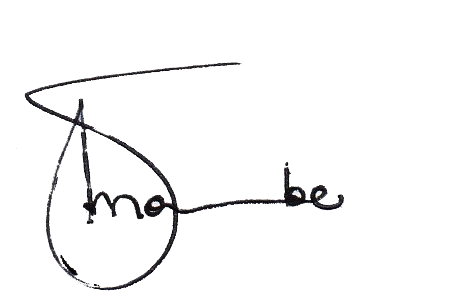
\includegraphics[viewport = 0 107 350 50,width=12cm]{./plots/signature.png}
	\end{figure}  

	\vspace {0.6in}
	\textbf{Signature}:\makebox[1.9in]{\hrulefill} \hspace{1.3in}\textbf{Date: \today} \\
\newpage
%%%%%%%%%%%%%%%%%%%%%%%%%%%%%%%%%%%%%%%%%%%%%%%%%%%%%%%%%%%%%%%%%%%%%%%%%%%
%%%%%%%%%%%%%%%%%%     The acknowledgements page         %%%%%%%%%%%%%%%%%%  
%%%%%%%%%%%%%%%%%%%%%%%%%%%%%%%%%%%%%%%%%%%%%%%%%%%%%%%%%%%%%%%%%%%%%%%%%%%
%\chapter*{Research output}
%\thispagestyle{empty}
%\addcontentsline{toc}{chapter}{\numberline{}Acknowledgements} 
%This thesis is based on three manuscripts:

%\begin{table}[h]
%\resizebox{\textwidth}{!}{%
%\begin{tabular}{@{}ll@{}}
%\toprule
%\textbf{Manuscript}                                                                                              %                                                                                                                 %                             & \textbf{Publication outcome}                                                      %                                             \\ \midrule
%\multicolumn{1}{|l|}{\textit{\begin{tabular}[c]{@{}l@{}}1. Using shrinkage estimators to reduce bias\\  and MSE %in estimation of heavy tails \\ (Beirlant, J., Maribe, G. and Verster, A., 2017)\end{tabular}}}                  %%                             & \multicolumn{1}{l|}{Accepted (fourthcoming) by REVSTAT}                          %                                              \\ \midrule
%\multicolumn{1}{|l|}{\textit{\begin{tabular}[c]{@{}l@{}}2. Penalised bias reduction in extreme value \\ %estimation for censored Pareto-type data, \\ and long-tailed insurance applications \\ (Beirlant, J., Maribe, G. %and Verster, A., 2018)\end{tabular}}} & \multicolumn{1}{l|}{\begin{tabular}[c]{@{}l@{}}Accepted and published by %\\ Insurance: Mathematics and Economics\end{tabular}} \\ \midrule
%\multicolumn{1}{|l|}{\textit{\begin{tabular}[c]{@{}l@{}}3. Bias Reduced Peaks over Threshold Tail Estimation\\ %(Beirlant, J., Maribe, G., Ph. Naveau and Verster, A., 2018)\end{tabular}}}                                      %                               & \multicolumn{1}{l|}{\begin{tabular}[c]{@{}l@{}}Submitted to \\ Computational %Statistics \& Data Analysis\end{tabular}}         \\ \bottomrule
%\end{tabular}%
%}
%\end{table}
%\newpage
%%%%%%%%%%%%%%%%%%%%%%%%%%%%%%%%%%%%%%%%%%%%%%%%%%%%%%%%%%%%%%%%%%%%%%%%%%%
%%%%%%%%%%%%%%%%%%     The acknowledgements page         %%%%%%%%%%%%%%%%%%  
%%%%%%%%%%%%%%%%%%%%%%%%%%%%%%%%%%%%%%%%%%%%%%%%%%%%%%%%%%%%%%%%%%%%%%%%%%%
\chapter*{Acknowledgements}
\thispagestyle{empty}
\addcontentsline{toc}{chapter}{\numberline{}Acknowledgements} 
I would firstly like to thank \textbf{God} for all the blessings he has showered upon me and my family, for the daily strength he has given me and for all the people he has placed in my path to make life more meaningful.
\\\\
To my family for all the sacrifices they had to make for my education. Again to my family and friends for being understanding and having to deal with my ``research moods", most especially \textbf{Kgabo Mphahlele}.
\\\\
Towards the end of the term in November of 2014, I found myself in \textbf{Andréhette Verster's} office, seeking mentorship for my Honours research project. Not knowing she would continue to mentor me throughout my masters and PhD studies. This visit to her office has been one of the most fruitful endeavours of my life. I am truly grateful to have been called your student.
\\\\
To \textbf{Jan Beirlant} from {\it KU Leuven, Belgium}, a great teacher and mentor. From you, I have learned a lot about myself. I would like to thank you for taking out your time to work with me. I jokingly like to refer to you as my grandfather \smiley{}, this is because no one has ever had so much patience in explaining difficult concepts to me as you have. I am truly grateful for the life long contribution you have made in my life.
\\\\
To \textbf{Philippe Naveau} from \textit{Laboratoire des Sciences du Climat et de l'Environnement, CNRS, Université Paris-Saclay}, thank you for our collaborative work described in Chapter 5, and for being a fantastic host on our visit to Paris.
\\\\
I would also like to take pleasure in thanking \textbf{Sean van der Merwe} for his valuable advice concerning the Bayesian implementations in Chapter 3.
\\\\
A special thanks goes out to \textbf{Rym and Julien Worms} for their helpful discussions and suggestions on the topic of tail estimation for randomly censored data. 
\\\\
I would also like to thank and acknowledge the UFS High-Performance Computing (HPC) unit for providing me with the massive amount of computing resources I used to conduct simulation studies. More especially \textbf{Stephanus Riekert}, I am truly grateful for all the technical support you provided me.
\\\\
Thanks to the REVSTAT as well as Insurance: Mathematics \& Economics referees for their constructive comments which improved the presentation of the accepted papers significantly. I extend this thanks to the assessors taking out their invaluable time to asses this PhD thesis.
\\\\
I would lastly like to thank the ``\textit{SASA‐NRF GRANT: Academic statistics bursary fund}" for sponsoring this PhD research.

\textit{This work is based on the research supported wholly/in part by the National Research Foundation of South Africa (Grant Number 102628). The Grantholder acknowledges that opinions, findings and conclusions or recommendations expressed in any publication generated by the NRF supported research is that of the author(s), and that the NRF accepts no liability whatsoever in this regard.}\newpage
\cleardoublepage
%%%%%%%%%%%%%%%%%%%%%%%%%%%%%%%%%%%%%%%%%%%%%%%%%%%%%%%%%%%%%%%%%%%%%%%%%%%%
%%%%%%%%%%%%%%%%%%         List of acronyms              %%%%%%%%%%%%%%%%%%  
%%%%%%%%%%%%%%%%%%%%%%%%%%%%%%%%%%%%%%%%%%%%%%%%%%%%%%%%%%%%%%%%%%%%%%%%%%%
\chapter*{List of acronyms}
\thispagestyle{empty}
\addcontentsline{toc}{chapter}{\numberline{}List of acronyms}
\begin{tabular}{p{3cm}p{8cm}}
\textbf{2ERV} & Second order extended regular variation\\
\textbf{CH} & Corrected Hill \\
\textbf{CLT} & Central limit theorem\\
\textbf{CDF} & Cumulative distribution function\\
\textbf{IID} & Independent, identically distributed\\
\textbf{EP}  & Extended Pareto\\
\textbf{EPD}  & Extended Pareto distribution \\
\textbf{ERV} & Extended regular variation\\
\textbf{EVI} & Extreme value index\\
\textbf{EVT} & Extreme value theory\\
\textbf{GEV} & Generalised extreme value\\
\textbf{GP} & Generalised Pareto\\
\textbf{GPD} & Generalised Pareto distribution\\
\textbf{HTE} & Heavier than exponential\\
\textbf{KM} & Kaplan-Meier\\ 
\textbf{LTE} & Lighter than exponential\\
\textbf{ML} & Maximum likelihood\\
\textbf{MLE} & Maximum likelihood estimate\\
\textbf{MVBR} & Minimum variance reduced bias\\
\textbf{PML} & Penalised maximum likelihood\\
\textbf{POT} & Peaks over threshold\\
\end{tabular}
\clearpage
\cleardoublepage

%%%%%%%%%%%%%%%%%%%%%%%%%%%%%%%%%%%%%%%%%%%%%%%%%%%%%%%%%%%%%%%%%%%%%%%%%%%
%%%%%%%%%%%%%%%%%%         Mathematical notations        %%%%%%%%%%%%%%%%%%  
%%%%%%%%%%%%%%%%%%%%%%%%%%%%%%%%%%%%%%%%%%%%%%%%%%%%%%%%%%%%%%%%%%%%%%%%%%%
\chapter*{Mathematical notation}
\thispagestyle{empty}
\addcontentsline{toc}{chapter}{\numberline{}Mathematical notation}
\begin{tabular}{p{4cm}p{12cm}}
$\gamma$ & Extreme value index.\\
$\mathcal{D}(G_{\gamma})$ & Domain of attraction of $G_{\gamma}$.\\
$\mathcal{F}$ & Class of distributions in the Fréchet domain of attraction.\\
$F^{\leftarrow}$ &	left continuous inverse of the distribution function $F$.\\
$f\in RV_{\rho}$ & $f$ is regular varying with index $\rho$.\\
$\Delta$ & Censoring indicator, 0 if the observation is right-censored and 1 if not.\\
$\l_{pen}$ & Penalised likelihood.\\
$\blacktriangle$ & Indicates the end of a definition, proof, lemma or proposition.\\
$\ell_{a}, \ell_{\delta}, \ell_U$ \& $\ell_U$ & Slowly varying functions.\\
$f\in 2ERV_{\gamma,\rho}$ &  $f$ is of second order extended regular variation.\\
$Q(p)$ & The quantile function denoted by $Q(p)=\inf\{x|F(x)\geq p\}$.\\
$H_{k,n}$ & The Hill estimator based on $k$ excesses above the threshold.\\
$t\uparrow \infty$ & $t$ approaches $\infty$ from below, in an increasing manner.\\
$\to^d \mathcal{N}_p$ & Converges in distribution to a $p$ dimensional Normal.\\
$\omega$ & Tuning constant regulating the amount of penalty.\\
$E_{\infty},\ Var_{\infty}\ \ \&\ MSE_{\infty}$ & Asymptotic bias, variance and mean squared error.\\
${\cal T}$ and ${\cal E}$ & Transformed and extended models.
\end{tabular}
\cleardoublepage
%%%%%%%%%%%%%%%%%%%%%%%%%%%%%%%%%%%%%%%%%%%%%%%%%%%%%%%%%%%%%%%%%%%%%%%%%%%
%%%%%%%%    tableofcontents, listoffigures and listoftables       %%%%%%%%%
%%%%%%%%        Command if you do not have  them                  %%%%%%%%%
%%%%%%%%%%%%%%%%%%%%%%%%%%%%%%%%%%%%%%%%%%%%%%%%%%%%%%%%%%%%%%%%%%%%%%%%%%%
\tableofcontents
\newpage
\listoffigures
\newpage
\listoftables
\newpage
\clearpage

\newpage
%%%%%%%%%%%%%%%%%%%%%%%%%%%%%%%%%%%%%%%%%%%%%%%%%%%%%%%%%%%%%%%%%%%%%%%%%%%
%%%%%%%%%%%%%%%%%%%%%%   END OF FRONT PAGE %%%%%%%%%%%%%%%%%%%%%%%%%%%%%%%%
%%%%%%%%%%%%%%%%%%%%%%%%%%%%%%%%%%%%%%%%%%%%%%%%%%%%%%%%%%%%%%%%%%%%%%%%%%%

%% To ensure the equation counter works correctly
\setcounter{page}{1}
\eqlabon
\eqlaboff
\pagenumbering{arabic}

\setcounter{equation}{0}
\chapter{Introduction}
\epigraphfontsize{\small\itshape}
\epigraph{``\textit{Nothing is more self-limiting than going to extremes}.''}{--- Marty Rubin}
\vspace{2.8cm}
\noindent
At the forefront of philosophical discourses in statistics, was the measure of central tendency of a population (the average). The inquiry of the ``limiting" distribution of a sequence of random variables would later lead up to the first version of what is known as the Central Limit Theorem (CLT) which appeared in 1733, by the French-born mathematician Abraham de Moivre. 

The CLT is perhaps the most fundamental result in all of statistics. It provides a theoretical framework that allows for justification of inference to extrapolate from a sample and make good approximations and predictions. Under some conditions the CLT states that the normal distribution (Gaussian) appears as a limiting distribution of the sample averages when the number of observations is sufficiently large. 

A corresponding discourse which emerged in the 20th century, was that of the maxima rather than the average. {\it What appears as the limiting distribution of the partial maxima ?}

This question has led to a very fruitful and path-breaking intellectual pursuit, the development of a theoretical framework known as Extreme Value Theory (EVT). Most concur that it made a first appearance in a paper by \cite{dodd1923greatest}, followed quickly by the papers of \cite{frechet1927} and \cite{fisher1928limiting}.

EVT has a rich mathematical theory which helps us answer non-trivial inferential questions about extreme observations and is applicable to a vast number of disciplines. The goal is often motivated by the need to predict the upper quantile or tail probability. Areas of application include but is not limited to: climatology, finance, insurance, survival analysis, hydrology and geology.

\section{Purpose of study and contributions}
The main research focus in EVT has over the past half-century taken a dramatic change. Peaks over threshold (POT) methods based on large observations (herein referred to as excesses) above some suitably high threshold have become more popular since the pioneering work of \cite{balkema1974residual} and \cite{pickands1975statistical}. The use of POT methods however prompt the question: ``what is a suitable threshold?" Issues with threshold selection are discussed in Section \ref{thresholdsection}. Work presented in this thesis is meant to subjugate the sensitivity inherent in threshold selection.

A second-order refined model makes use of additional information up to the second-order about the slowly varying function $\ell$. \cite{sts626} proposed a quantile and probabilistic view of second-order refinements for $\gamma>0$ estimators. In the first part of this PhD thesis, we propose some improvements to second order refinements made by \cite{beirlant2009second} by using the theoretical fact that, for large thresholds the distribution of excesses is strictly Pareto, leading to a shrinkage estimation technique of the extreme value index (EVI).

Motivated by applications for instance in actuarial statistics, the subject of censoring in heavy-tailed data has received growing attention in EVT. This thesis reviews some existing tail estimation methods and proposes a second order improved version of the \cite{worms2014new} estimator.

Second order models naturally add some restrictions. This thesis further proposes a bias reduced tail fitting technique that allows for these restrictions to be relaxed. The second order refined POT approach started in \cite{beirlant2009second} is revisited and extended to all max-domains of attraction by applying a flexible semi-parametric modelling of the second order component.

\section{Thesis Objectives}
\begin{itemize}
    \item Propose a shrinkage estimation technique to reduce the mean squared error (MSE) of the Extended Pareto distribution (EPD) of \cite{beirlant2009second};
    \item Propose a bias reduced version of the \cite{worms2014new} estimator;
    \item Construct confidence intervals of the bias reduced \cite{worms2014new} using a bootstrap algorithm;
    \item Propose a novel bias reduced tail fitting technique for all max-domains of attractions.
\end{itemize}
\section{Outline of Thesis}
This thesis is divided into two parts, \autoref{part1} focuses on second order refinements for censored and uncensored heavy-tailed distributions. \autoref{part2} reviews attempts made to build flexible full models capable of capturing the bulk and tail part of the data. A novel semi-parametric refinement is proposed in this part.

\autoref{chap2} gives an overview of EVT, introduces some key concepts and mentions historical developments in the field. 
In \autoref{chap3} we introduce a shrinkage estimation technique to improve an unbiased estimator of the EVI and reduce the overall MSE. The overall reduction in MSE is shown both mathematically and through a finite simulation study. A short case study is conducted on a Secura Belgian Reinsurance data set.

In \autoref{chap4} we focus on random right censored heavy tailed data, and propose a bias reduced version of the \cite{worms2014new} estimator. We then apply the shrinkage technique introduced in \autoref{chap3} to improve MSE of this newly proposed estimator. A finite simulation study and a long tailed insurance application are conducted.

In \autoref{chap5}, the second order bias reduction technique is extended to all domains of attraction. A general form of the second order refined model is proposed. Merits of the proposed estimators are illustrated with a case study on a rain fall data set. An interactive simulation study is conducted and hosted on a shiny-website provided at the end of the chapter.

In \autoref{chap6}, a conclusion of the study is presented, and some areas which allow for further research are identified.
\newpage

\section{Authorship and publication}
Some parts of this thesis are based on work by the author already published in international peer reviewed journals. Below is the list of published and publishable journal papers listed in chronological order as presented in chapters to follow.

\begin{enumerate}
    \item Beirlant, J., Maribe, G. and Verster, A., 2019. Using shrinkage estimators to reduce bias and MSE in estimation of heavy tails. \textit{REVSTAT–Statistical Journal}, 17(1), pp.91-108.
    
    \item Beirlant, J., Maribe, G. and Verster, A., 2018. Penalized bias reduction in extreme value estimation for censored Pareto-type data, and long-tailed insurance applications.\textit{ Insurance: Mathematics and Economics}, 78, pp.114-122.
    
    \item Beirlant, J., Maribe, G., Naveau, P. and Verster, A., 2018. Bias Reduced Peaks over Threshold Tail Estimation. \textit{arXiv preprint arXiv:1810.01296.}
\end{enumerate}
\nocite{beirlant2017using}
\nocite{beirlant2018penalized}
\nocite{beirlant2018bias}
\newpage
\chapter{Background}\label{chap2}
\section{Introduction}
EVT is primarily concerned with the limiting distribution of the maxima or minima of independent, identically distributed (IID) random variables.

Let $X$ be a arbitrary random variable with a cumulative distribution function (CDF) $F$. Moreover, let $X_1,X_2,...,X_n$ be IID random variables. The ordered set is then denoted as $X_{1,n} \leq X_{2,n} \leq...\leq X_{n,n}$. The limit problem is that of finding a potential limiting distributions of the maximum $X_{n,n} = \max(X_1,X_2,...,X_n)$. The distribution of this sample maximum can be written as $P(X_{n,n} \leq x) = F^n(x)$, non trivially for some constants $a_n>0$ and $b_n$: 
\begin{equation}\label{cond1}
F^n(a_n x+b_n) \rightarrow^d G(x), \text{ weakly as } n\rightarrow \infty.
\end{equation}thereby reducing the limit problem to a location and scale problem where $G(x)$ is one of the three possible limiting distribution functions. 

This problem was initially solved by \cite{fisher1928limiting}, and later derived rigorously by \cite{gnedenko1943distribution} and further streamlined by \cite{dehaan1970regular}. The extremal types theorem asserts that if a non-degenerate $G$ exists it must be one of three types:
\begin{eqnarray*}
I&:& \Lambda (x) = \exp\{-e^{-x}\},\ \ \ x\in\mathbb{R}: \\
II&:& \Phi_{\alpha}(x) =
\begin{cases}
 0, & \ x\leq 0 \\
 \exp\{-x^{-\alpha}\}, & \ x>0
\end{cases}
\\&& \text{for some}\ \alpha >0\\
III&:& \Psi(x) =
\begin{cases}
 \exp\{-(-x)^{\alpha}\}, & \ x\leq 0 \\
 1, & \ x>0
\end{cases}
\\&& \text{for some}\ \alpha >0
\end{eqnarray*}
\begin{figure}[h!]
\centering
	\begin{subfigure}[h]{0.49\linewidth}
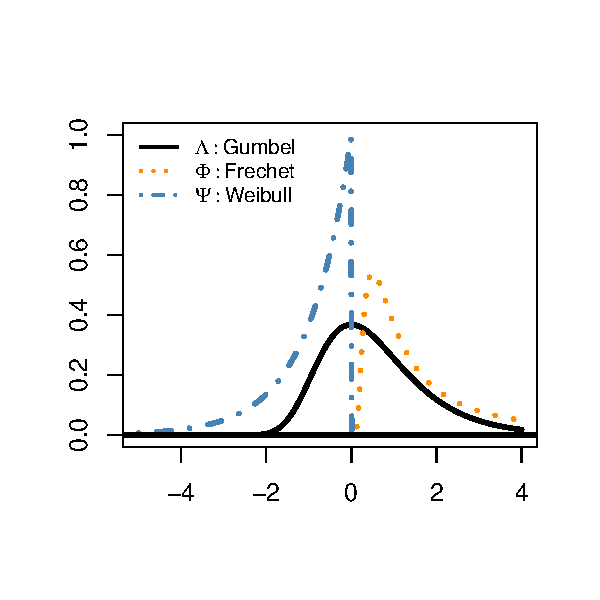
\includegraphics[width=\textwidth]{./plots/chapter2_plots/densities1.pdf}
\end{subfigure}
	%	\hspace{0.1\fill}
			\begin{subfigure}[h]{0.49\linewidth}
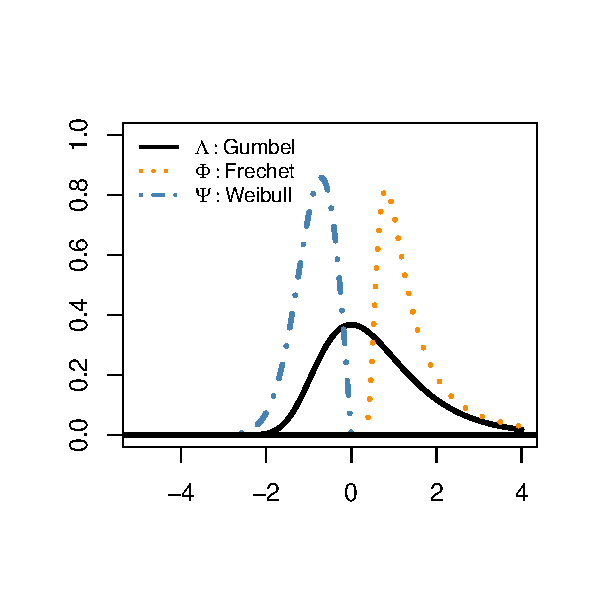
\includegraphics[width=\textwidth]{./plots/chapter2_plots/densities2.pdf}
\end{subfigure}
\caption{Densities of the three standard extreme value distributions. With $\alpha = 1$ (left) and $\alpha = 2$ (right)}
\label{fig:my_label}
\end{figure}

These types of distributions are often referred to as the Gumbel, Fréchet and Weibull types, respectively.
The three types of distributions can be joined into a single distribution function with the following cumulative distribution function (CDF):
\begin{equation}\label{gev1}
G_{\gamma}(x) = 
\begin{cases}
 \exp\left\{ -\left( 1+\gamma x \right)^{-1/\gamma} \right \}, & \text{if}\ \gamma\neq0 \\
 \exp\left\{-e^{-x} \right\}, & \text{if}\ \gamma=0
\end{cases}
\end{equation}defined on $\{x: 1+\gamma x > 0\}$ and $\gamma \in \mathbb{R}$.
This CDF is known as the Generalised Extreme value (GEV) distribution. The parameters $\gamma$ is known as the shape parameter, also known as the EVI. This parameter is of primordial importance in EVT.

\begin{figure}[h!]
\centering
	\begin{subfigure}[h]{0.49\linewidth}
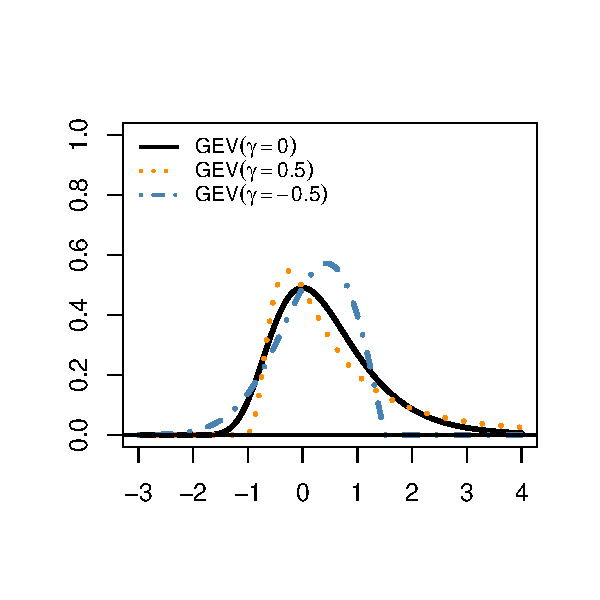
\includegraphics[width=\textwidth]{./plots/chapter2_plots/gevdensity1.pdf}
\end{subfigure}
	%	\hspace{0.1\fill}
			\begin{subfigure}[h]{0.49\linewidth}
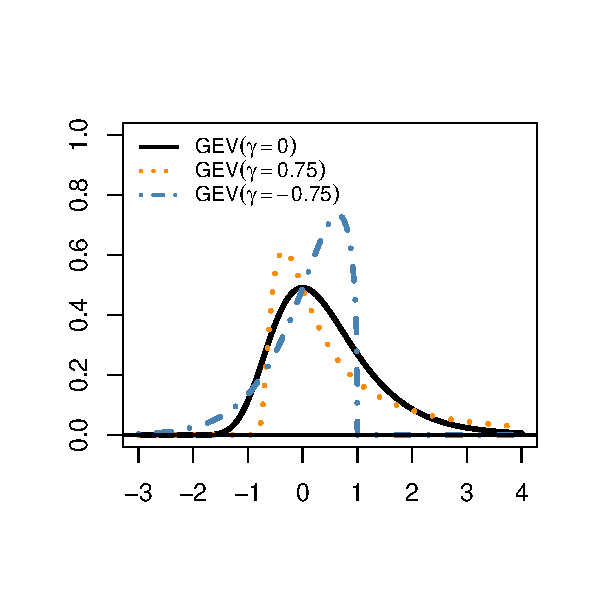
\includegraphics[width=\textwidth]{./plots/chapter2_plots/gevdensity2.pdf}
\end{subfigure}
\caption{Densities of the $GEV(\gamma)$ with $\gamma$ choices: 0,0.5,-0.5 (left) and 0,0.75,-0.75 (right)}
\label{gev}
\end{figure}
It becomes clear from Figure \ref{gev} that the EVI affects the tail behaviour. If $\gamma = 0$, the GEV distribution decays exponentially and belongs to the Gumbel family. If $\gamma > 0$, the GEV distribution has a much heavier tail and belongs to the Fréchet family. Lastly if $\gamma < 0$, the GEV has a finite upper endpoint and belongs to the Weibull family.

If (\ref{cond1}) holds, we can say that the underlying distribution $F$ is in the domain of attraction of $G_{\gamma}$ and write $F\in \mathcal{D}(G_{\gamma})$. This is the set of distributions attracted to $G_{\gamma}$. For example it can be shown that the Loggamma distribution is in the domain of attraction of $G$ with $\gamma > 0$.

The rigorous mathematical framework provided by EVT necessitates some assumptions about regularity conditions for the underlying distributions. Throughout the different parts of this thesis we refer to the well known, necessary and sufficient conditions for $F\in \mathcal{D}(G_{\gamma})$. Without going into much detail we therefore make a brief overview of the necessary and sufficient conditions in order to give a preliminary context.

Define the support of a distribution function $F$ by the lower bound ${}_{+}x := \sup\{x: F(x)=0\}$ and the upper bound $x_+ := \inf\{x: F(x)=1\}$. The quantile function $Q(y)=F^{\leftarrow}(y)=\inf\{x: F(x)\geq y \}$ and the tail quantile function $U(y) = F^{\leftarrow}\left( 1-\dfrac{1}{y} \right)$.
%###########################################################################################################

\subsection*{First-Order Condition}\\
Consider the underlying distribution function $F$ underlying in the extremal domain of attraction of the GEV distribution, $F\in \mathcal{D}(G_{\gamma})$.
There exists a positive measurable function $a$ for which \citep{de1984slow}:
\begin{equation}\label{condition1}
\lim_{t\rightarrow\infty} \dfrac{U(tx)-U(t)}{a(t)} = D(x) =
\begin{cases}
\dfrac{x^{\gamma}-1}{\gamma}\ \ &\text{if } \gamma \neq 0\\
\log(x)\ \ &\text{if } \gamma \neq 0
\end{cases}
\end{equation}for all $x > 0$.

\cite{de1984slow} shows that Equation (\ref{condition1}) is equivalent to the following statement:\\
{\it There is a positive function $a$ such that:}
\begin{equation}\label{condition1b}
\lim_{t\rightarrow\infty} t(1-F(a(t)x + U(t))) = (1+\gamma x)^{-1/\gamma}
\end{equation}{\it for all $x$ with }$1+\gamma x >0$.\\
\hspace*{\fill}$\blacktriangle$

\begin{definition}\textnormal{\textbf{Regular variation}} \\
	All functions ultimately zero are said to belong to a class of regular varying functions if:\begin{equation}
	\lim\limits_{t\rightarrow \infty}\dfrac{f(tx)}{f(t)}=x^{\rho},\ \ \ \text{for}\ x>0, \text{with some } \rho \in \mathbb{R},
	\end{equation}$f$ is said to be regular varying with index $\rho$, $f\in RV_{\rho}$. Furthermore a function $f$ is said to be slowly varying if for $x>0$: \begin{equation}
	\lim\limits_{t\rightarrow \infty}\dfrac{f(tx)}{f(t)}=1.
	\end{equation}
\end{definition}

\subsection*{Second-Order Condition}
\subsubsection*{A general tail ($\gamma\in\mathbb{R}$)}
$F$ satisfies the second order condition if there exists a function $A(t)$, tending to zero as $t\rightarrow\infty$, such that:
\begin{equation}\label{2nd}
\lim\limits_{t\rightarrow\infty}\dfrac{\dfrac{U(tx)-U(t)}{a_0(t)}-\dfrac{x^{\gamma}-1}{\gamma}}{A(t)}=H_{\gamma,\rho}(x):=\dfrac{1}{\rho}\left(\dfrac{x^{\gamma+\rho}-1}{\gamma+\rho}-\dfrac{x^{\gamma}-1}{\gamma}\right)
\end{equation}
for all $x>0$ and $a_0>0$, with $\rho <0$, the second order parameter controlling the speed of convergence of the partial maxima towards the limit law. It is then said that the function $U$ is of second order extended regular variation, and write $U\in 2ERV_{\gamma,\rho}$, noting also that, $|A|\in RV_{\rho}$ and tends to zero, hence larger absolute values of $\rho$ correspond to a higher rate of convergence.

\subsubsection*{A heavy tail ($\gamma>0$)}
In case of heavy tails the second order condition reads as follows. The existence of the function $\tilde{A}(t)$ is such that:
\begin{equation}
\begin{array}{ll}
\lim\limits_{t\rightarrow\infty}\dfrac{\dfrac{U(tx)}{U(t)}-x^{\gamma}}{\tilde{A}(t)}&=x^{\gamma}\dfrac{x^{\tilde{\rho}}-1}{\tilde{\rho}}\Longleftrightarrow\\& \lim\limits_{t\rightarrow\infty}\dfrac{\ln U(tx)-\ln U(t)-\gamma\ln x}{\tilde{A}(t)}=\dfrac{x^{\tilde{\rho}}-1}{\tilde{\rho}}
\end{array}
\end{equation}
for all $x>0$, and $\tilde{\rho}\leq 0$, the second order parameter. As in the general case, we then say $U$ is of second order regular variation and write $U\in 2RV_{\gamma,\tilde{\rho}}$. $F$ is said to satisfy the second order condition \citep{alves2007note}.
\hspace*{\fill}$\blacktriangle$

There is a special class of Pareto type distributions, known as the Hall class. This is a wide class of models containing most useful heavy-tailed parents such as those used in this thesis, namely: the Fréchet and the Burr XII distribution.\\
\begin{definition}\label{hall}\textnormal{\textbf{Hall class of distributions}}\ \\
	Assuming the underlying distribution $F$ satisfies $F(0)=0$, the survival function of a distribution in the Hall class \citep{hall,welsh} can be written as:
	\begin{equation}\label{hallclassF}
		\bar{F}(t)=C^{1/\gamma}t^{-1/\gamma}[1+\gamma^{-1}DC^{\rho/\gamma}t^{-\rho/\gamma}+o(1)],\ \ t\uparrow \infty, 
	\end{equation} where $\gamma >0, C>0, \rho<0$ and $D\in\mathbb{R}$.\\
\end{definition}

For any $\tau=\rho/\gamma$ and $C^{1/\gamma}\propto C$, we can write (\ref{hallclassF}) as:
\begin{equation}\label{F}
	1-F(x)=Cx^{-\alpha}[1+Dx^{\tau}+o(x^\tau)],\ \ \ x\uparrow \infty, 
\end{equation} where $\alpha >0, C>0, \tau<0$ and $D\in\mathbb{R}$.
\autoref{F} can also be written as a tail quantile function: \begin{equation}
	U(t)=Ct^{\gamma}\left(1+\dfrac{A(t)}{\rho}+o(t^{\rho})\right),\ \ \ A(t)=\gamma\tau t^{\rho}.
\end{equation}

Much more insightful readings on second order conditions and regular variation can be found in the famous work of \cite{de1996generalized}. \cite {alves2007note} also 
provides a very comprehensive overview of the first, second and third order conditions. In this thesis we do not make use of this third order frame work. Furthermore a detailed explanation of the characterisation of normalising constants $a_n$ and $b_n$ more specific to the first order condition, can be found in \cite{leadbetter2012extremes}. Table \ref{domain}\footnote{Table \ref{domain} is adapted from \cite{albrecher2017reinsurance}} provides a short list of some of the very common distribution functions classified according to the different domains.

%###########################################################################################################

\begin{table}[h]
\centering
\begin{tabular}{llll} 
\toprule
\textbf{Domain } & \textbf{Distribution } & $1-F(x)$& $({}_{+}x,x_+)$ \\ 
\hline
\multirow{3}{*}{\begin{tabular}[c]{@{}l@{}}Weibull \\$\gamma < 0$ \end{tabular}} & Reversed Burr & $\beta^{\alpha}(\beta+x_{*}-x)^{-\tau})^{-\alpha}$ & $(0,x_{*})$ \\
 & Extreme Weibull& $1-e^{-(1-x)^{\alpha}}$& $(0,x_{*})$ \\
 & Beta& $\dfrac{1}{B(p,q)}\int^1_x u^{p-1}(1-u)^{q-1}$ & $(0,1)$ \\ 
\hline
\multirow{3}{*}{\begin{tabular}[c]{@{}l@{}}Gumbel \\$\gamma = 0$ \end{tabular}} & Gamma & $\dfrac{\lambda^{\alpha}}{\Gamma(\alpha)}\int^{\infty}_x e^{-\lambda u}du$ & ($0,\infty$) \\
 & Exponential& $e^{-\lambda x}$& ($0,\infty$) \\
 & Log Normal & $\int^{\infty}_x \dfrac{1}{\sqrt{2\pi}\sigmat}\exp\left( -\dfrac{1}{2\sigma^2}(\log u-t)^2 \right) du$ & ($0,\infty$) \\ 
\hline
\multirow{3}{*}{\begin{tabular}[c]{@{}l@{}}Fréchet\\$\gamma > 0$ \end{tabular}} & Strict Pareto & $(x/x_0)^{-\alpha}$& $(x_0,\infty)$\\
 & Burr (XII) & $\beta^{\alpha}(\beta+x^{\tau})^{-\alpha}$ & $(0,\infty)$ \\
 & Log-gamma & $\int^{\infty}_x \dfrac{\lambda^{\alpha}}{\gamma(\alpha)} u^{-\lambda - 1} \log(u)^{\alpha-1} du$& $(1,\infty)$ \\
\hline
\end{tabular}
\caption{A list of some common distributions and their respective domains of attraction }
\label{domain}
\end{table}

\section{Motivating data set}\label{mtplsection}
In order to demonstrate the need for EVT and methods proposed in this thesis, a simplified case study in reinsurance is considered. 
\subsection{Reinsurance: Motor Liability Data}
We present in this section a motor third-party liability (MTPL) data set first studied by \cite{albrecher2017reinsurance}.
This data contains 849 insurance European claims between 1995 and 2010 evaluated on 1 January 2011. 59\% of these claims were not closed at the time of evaluation. To account for inflation and reflect costs in the calendar year 2011, all amounts have been indexed.
\\\\
In order to make claim reservations, insurance companies will have experts approximate the ultimate losses still under development alongside aggregate payments and incurred losses. In case a claim is closed during the study period, the ultimate value is then the aggregate payment.
\begin{figure}[h!]
\centering
	\begin{subfigure}[h]{0.49\linewidth}
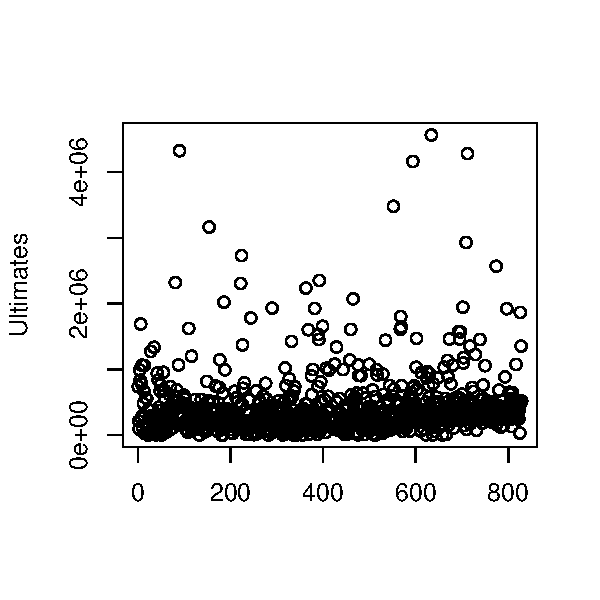
\includegraphics[width=\textwidth]{./plots/chapter2_plots/ultimates.pdf}
\end{subfigure}
	%	\hspace{0.1\fill}
			\begin{subfigure}[h]{0.49\linewidth}
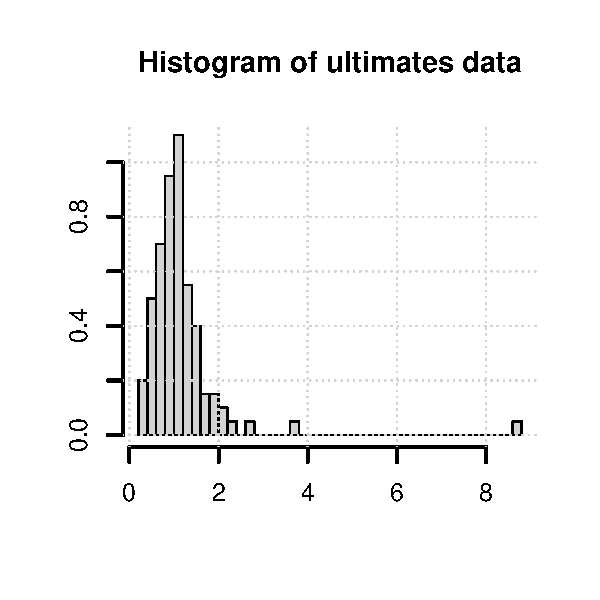
\includegraphics[width=\textwidth]{./plots/chapter2_plots/mtpl_dens.pdf}
\end{subfigure}
\caption{Scatter plot of ultimates loss data (left) and the corresponding empirical density plot (right)}
\label{fig:hist}
\end{figure}
\begin{table}[h]
\centering
\resizebox{\linewidth}{!}{%
\begin{tabular}{llllll} 
\hline
\textbf{min} & \textbf{1st~quartile} & \textbf{median} & \textbf{mean} & \textbf{3rd~quartile} & \textbf{max} \\ 
\hline
90& 167,389& 286,296 & 422,435& 485,973& 4,564,759\\
\hline
\end{tabular}
}\caption{Summary of the ultimates data}
\label{chap2:tab1}
\end{table}
\\\\
For now we shall work with the ultimate loss projections and assume that they are IID. In order to aid us in identifying the claim size distribution type, we make a scatter-plot and histogram of the data in Figure \ref{fig:hist} and also make a summary table of the data in Table \ref{chap2:tab1}. 

Let us consider a situation in which the insurance company is interested in knowing the probability of getting a claim amount larger than say 1,000,000. Secondly, what is the claim amount that can be exceeded with a probability of 0.05. This situation can be solved by classical statistical techniques.

The CLT suggests that the empirical distribution of the data carries all the information needed for inference, this implies the inability to extrapolate beyond a given population sample. The solution is therefore straight forward since the sample size is large enough and the value 1,000,000 is within the sample. Now denote the random claim by $Y$, from the 849 claims we find that only 65 claims exceed 1,000,000. The probability can thus be estimated by $P(Y>1,000,000) \approx 65/849 = 0.077$.

To answer the second question we need a $95^{th}$ percentile of the underlying distribution i.e. the value of $y$ such that $P(Y>y) = 0.05$. We sort the data set by values from highest to lowest and discard the highest 5\% of the sorted data. The succeeding highest sample is then the $95^{th}$ percentile value for the data set. 849*0.95 = $\ceil{787.55} = 788$. This is the $788^{th}$ number in the ordered list, which is 1,352,780.
\\\\
We now consider a situation in which the insurance company is interested in knowing the probability of getting a claim amount larger than the largest claim amount. They might also be interested in knowing, what is the highest possible claim amount that may occur. Classical statistical methods begin to break down. For the first question: any value above the maximum is not observable and therefore the probability would be zero. A conventional statistical solution to the second problem is the maximum observable value contained in the sample. Insurance claims are known to be heavy-tailed and therefore both these answers are not plausible.

We can resort to EVT to answer these questions since it allows us to extrapolate beyond the given range of data. We can naively assert from Figure \ref{fig:hist} that this data set is heavy-tailed. There are of course more plausible graphical tools for this type of analysis. These are explained in Sections \ref{hill} and \ref{qq}.

For the first question, let $F$ be the distribution function of the ultimates. The problem is that of estimating $1-F(x)$ with $x$ large. Using Equation (\ref{condition1b}) it can then be restated as a tail probability for some large threshold $t$:
\begin{eqnarray*}
t(1-F(a(t)x + U(t))) &=& (1+\gamma x)^{-1/\gamma}\\
1-F(a(t)x + U(t)) &=& \dfrac{1}{t}\left(1+\gamma x\right)^{-1/\gamma}
\end{eqnarray*}
\begin{eqnarray*}
1-F\left(\dfrac{a(t)x + U(t) - U(t)}{a(t)}\right) &=& 1-F(x)\\
=\dfrac{1}{t}\left(1+\gamma \dfrac{x-U(t)}{a(t)}\right)^{-1/\gamma}.
\end{eqnarray*}Assuming that the data is indeed heavy-tailed and in the Fréchet domain ($\gamma>0$), \cite{sts626} show that a suitable choice of the function $a(t)$ can be $a(t)=\gamma t^{\gamma}\ell_U(t)= \gamma U(t)$ and thus:
\begin{eqnarray*}
1-F(x) &=& \dfrac{1}{t}\left(1+\gamma \dfrac{x-U(t)}{\gamma U(t)}\right)^{-1/\gamma}\\
&=& \dfrac{1}{t}\left(\dfrac{U(t)}{x}\right)^{1/\gamma} > 0.
\end{eqnarray*}
To get an estimate of this we can use:
\begin{eqnarray}
\hat{\bar{F}} = k/n \left( \hat{U}(n/k) \over x \right)^{1/\hat{\gamma}},
\end{eqnarray}where $n$ is the samples size, $k$ is the number of observations above the threshold, $\hat{\gamma}$ is an estimate of $\gamma$ and $\hat{U}(n/k)$ is an estimate of $U(t)$.

For the second question we need to find the right endpoint or tail quantile $F^{\leftarrow}(1)$=$U(\infty)$, in the $\gamma$ negative case.

Using (\ref{condition1}), for some positive measurable function $a$:
\begin{eqnarray*}
\lim_{t \rightarrow \infty} \dfrac{U(\infty) - U(t)}{a(t)} &=& \dfrac{x^{\gamma}-1}{\gamma} \rightarrow \dfrac{-1}{\gamma}\\
U(\infty) &=& U(t) - a(t)/\gamma.
\end{eqnarray*}This is only the case if the data set is short tailed ($\gamma < 0$). If the data is heavy-tailed, the right endpoint does not exist, i.e. $x_+ = U(\infty) = \infty$.
The insurance company will therefore resort to computing a risk measure known as value at risk (VAR), which in an extreme value context is a quantile value computed at a very small probability.
\\\\
It is clear by now that the parameter $\gamma$ plays a very important role in EVT. As will be seen in the next section. A significant amount of research has been dedicated to the estimation of this parameter. We can make use of graphical methods to assess the goodness of fit of the proposed distribution of the data.

To a great extent, interest in EVT has been statistical fits above high thresholds (the tails). As such quantile-quantile (QQ) plots and mean excess (mean residual life) plots are the most commonly used graphical tools since they are most informative for such purposes.

\subsection{Mean excess}\label{hill}
 The \textbf{Mean excess} function of a random variable $X$ is defined as: \begin{equation}
e_X(t)= E(X-t|X>t) = \dfrac{\int^{\infty}_t (1-F)(u)du}{1-F(t)}
\end{equation}provided that $\ E(X)<\infty$.

Estimates of the mean excesses for sample $X_1,...,X_n$ can be naively estimated by replacing the expectation by the empirical analogue, this yields:
\begin{equation}
 \hat{e}_{k,n}=\dfrac{\int^{\infty}_t \hat{\Bar{F}}(u)du}{\hat{\Bar{F}}(X_{n-k,n})} = \dfrac{1}{k}\sum_{j=1}^{k}X_{n-j+1,n}-X_{n-k,n}
\end{equation} where $\hat{\Bar{F}}$ is the empirical survival function and $t = X_{n-k,n}$ the threshold. The empirical function $\hat{e}_{k,n}$ is plotted against values $t=X_{n-k,n},k=1,...,n-1$, the $(k+1)^{th}$ largest observation.

Using the fact that $\log X$ is exponentially distributed with mean $\alpha$ when $X$ follows a strict Pareto, the mean excess function of the log transformed $X$ can be written as:
\begin{equation}
e_{\log X}(\log t)= E(\log X-\log t|X>t) = \dfrac{\int^{\infty}_t (1-F)(u)d\log u}{1-F(t)}.
\end{equation}Replacing again the expectation by the empirical analogue leads to the \cite{hill1975simple} statistic:
\begin{equation}
H_{k,n}=\dfrac{\int^{\infty}_t \hat{\Bar{F}}(u)d \log u}{\hat{\Bar{F}}(X_{n-k,n})} = \dfrac{1}{k}\sum_{j=1}^{k} \log X_{n-j+1,n}- \log X_{n-k,n}.
\end{equation}The Hill estimator is one of the most famous and computationally convenient estimator of $\gamma>0$.

The Mean excess can be very useful when determining a sufficient threshold for a plausible fit of a POT model. As the threshold increases, the plot may become more linear as the empirical distribution of excesses approach the POT model. Thus suggesting a choice of the threshold at the point above the non-linear portion of the plot.

\subsection{QQ-plots}\label{qq}
A QQ plot is a graphic tool used to test goodness of fit of a model to some sample population. The idea behind a QQ plot is that we can assess whether a particular model $F$ provides a good fit to the distribution of the random variable $X$ without having to estimate the location and scale parameters. If the model is a good fit, a plot of the ordered empirical quantiles $X_{1,n}\leq X_{2,n}\leq ...\leq X_{n,n}$ against the quantiles $Q(1/n),  Q(2/n),..., Q(n/n+1)$ associated with the proposed distribution function $F$ should be linear. This linear relationship can be captured by eye.

The \cite{hill1975simple} estimator can be retrieved through estimating the slope $1/\alpha$ of the regression line on a Pareto QQ plot.

\begin{table}[t]
\centering
\caption{Q-Q plot and derivatives plot coordinates.}
\resizebox{\linewidth}{!}{%
\begin{tabular}{l|lll} 
\cline{1-3}
\textbf{Distribution} & $\boldsymbol{F(x)}$ & \textbf{QQ Coordinates} & \\ 
\cline{1-3}
\textbf{Log-normal} & \begin{tabular}[c]{@{}l@{}}\\ $\int_{0}^{x}\dfrac{1}{\sqrt{2\pi \sigma t}}\exp\left(-\dfrac{(\log t-t)^2}{2\sigma^2}\right)du$ \\ $x>0;t\in\mathbb{R}, \sigma>0$ \end{tabular} & $\left(\Phi^{-1}(p_{i,n}),\log X_{i,n}\right)$ & \\ 
\cline{1-3}
\textbf{Exponential} & \begin{tabular}[c]{@{}l@{}}\\$1-\exp(-\lambda x)$~\\$x>0;\lambda>0$\end{tabular} & $\left(-\log(1-p_{i,n}),X_{i,n}\right)$~ ~ & \\ 
\cline{1-3}
\textbf{Pareto} & \begin{tabular}[c]{@{}l@{}}\\$1-x^{-\alpha}$~\\$x>1;\alpha>0$\end{tabular} & $\left(-\log(1-p_{i,n}),\log X_{i,n}\right)$ & \\ 
\cline{1-3}
\textbf{Weibull} & \begin{tabular}[c]{@{}l@{}}\\$1-\exp(-\lambda x^{\tau})$~\\$x>0;\lambda,\tau>0$~ ~\end{tabular} & $\left(\log(-\log(1-p_{i,n})),\log X_{i,n}\right)$ & \\
\hline
\end{tabular}
}
\label{qplots}
\end{table}

Other useful diagnostic plots that can be paired along with QQ plots are known as derivative plots \citep[see][for more details]{albrecher2017reinsurance}. Table \ref{qplots} \footnote{Table \ref{qplots} is adapted from \cite{sts626}} shows QQ plot coordinates for some distributions as given in \cite{sts626}. 

The corresponding derivative plot coordinates of the distributions in Table \ref{qplots} are given by:
\subsubsection*{Log-normal}
\begin{eqnarray*}
&&\left(\log X_{n-k,n}, \dfrac{H_{k,n}}{N_{k,n}} \right)\\
&&N_{k,n} = \dfrac{n+1}{k+1} \phi \left( \Phi^{-1}\left(1-\dfrac{k+1}{n+1}\right) \right)- \Phi^{-1}\left(1-\dfrac{k+1}{n+1}\right) 
\end{eqnarray*}$\phi$ denotes a standard normal density

\subsubsection*{Pareto}
\begin{equation*}
\left(\log X_{n-k,n}, H_{k,n}\right).
\end{equation*}

\subsubsection*{Weibull}
\begin{eqnarray*}
&&\left(\log X_{n-k,n}, \dfrac{H_{k,n}}{W_{k,n}} \right)\\
&&W_{k,n}=\dfrac{1}{k}\sum^k_{j=1}\log\log\dfrac{n+1}{j}-\log\log\dfrac{n+1}{k+1}.\\
\end{eqnarray*}

The derivative plot of the \textbf{Exponential} distribution is the Mean excess plot.
\\\\
As an initial step in extreme value analysis, it is important that we classify the tail of the distribution function $F$ as being exponential, heavier than exponential or lighter than exponential. The graphical diagnostics are summarised below.

\textbf{Lighter than exponential (LTE):}
\begin{itemize}
\item The exponential QQ plot will be ultimately convex tipping above the fitted regression line of the coordinates;
\item The Mean excess function will be ultimately increasing.
\end{itemize}

\textbf{Exponential tail:}
\begin{itemize}
\item The exponential QQ plot will be linear;
\item The Mean excess plot will be ultimately horizontal;
\item The Pareto QQ plot will be ultimately concave and tipping below the fitted regression line.
\end{itemize}

\textbf{Heavier than exponential (HTE):}
\begin{itemize}
\item The exponential QQ plot will be ultimately concave tipping below the fitted regression line of the coordinates;
\item The Mean excess plot will be ultimately decreasing;
\item The Pareto QQ plot will ultimately be linear
\end{itemize}
If however the practitioner is interested in determining whether the tail of the distribution function is Pareto, heavier than Pareto or lighter than Pareto, a similar approach can be taken replacing the Exponential QQ plot with a Pareto QQ plot and the Mean excess with a Pareto derivative plot. In an analogous manner, distributions in the Weibull domain can be inspected.

Diagnostic plots of the ultimates data set are given in Figure \ref{diagnostics}. These plots confirm that the data does in fact exhibit heavy tails.

It should be noted that data can have different regimes since the natural phenomena governing the process from which data is generated can vary. For example, the way an insurance company deals with small claims will be different from the way they deal with large claims. 

It can be seen in Figure \ref{diagnostics} that the ultimates loss projections appear to exhibit some form of a truncated regime for larger claims.

\begin{figure}[hh!]
	\begin{subfigure}[t]{0.45\textwidth}
		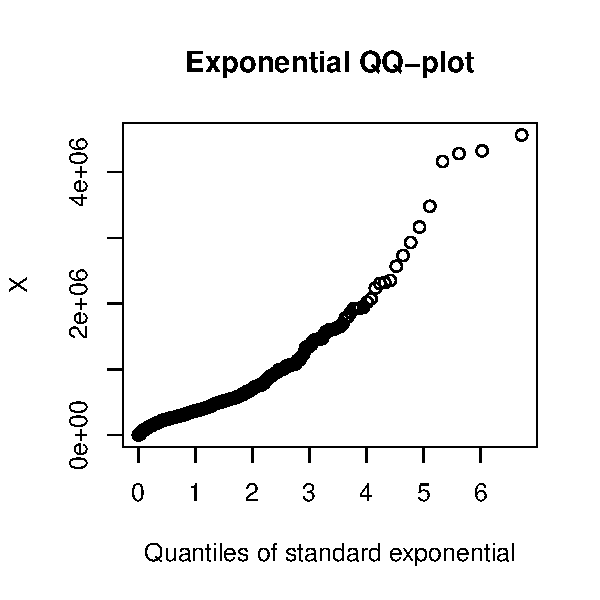
\includegraphics[width=\textwidth]{./plots/ExponentialQQ.pdf}
	\end{subfigure}
	\hfill
	\begin{subfigure}[t]{0.45\textwidth}
		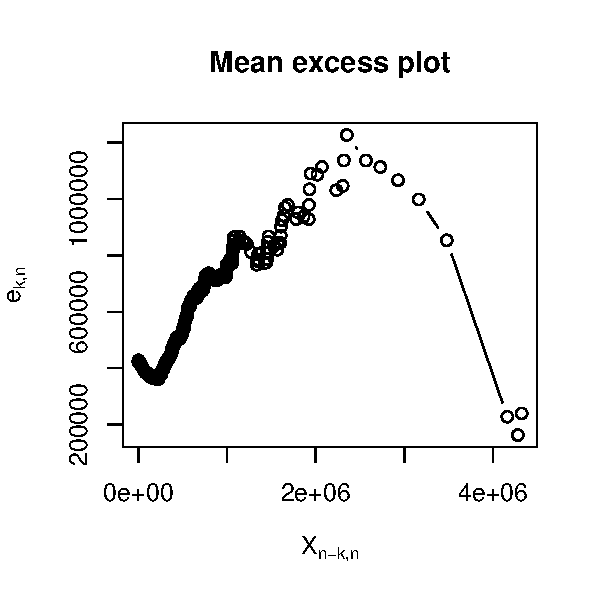
\includegraphics[width=\textwidth]{./plots/MeanExcess.pdf}
	\end{subfigure}
		\begin{subfigure}[t]{0.45\textwidth}
		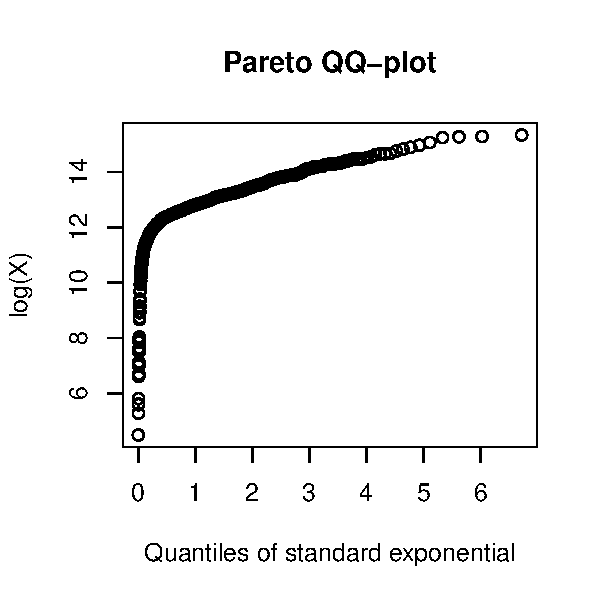
\includegraphics[width=\textwidth]{./plots/ParetoQQ.pdf}
	\end{subfigure}
		\hfill
		\begin{subfigure}[t]{0.45\textwidth}
		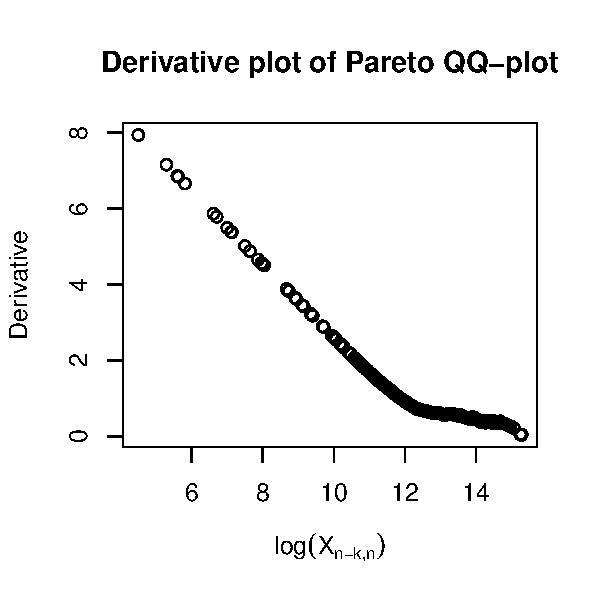
\includegraphics[width=\textwidth]{./plots/ParetoQQ_der.pdf}
	\end{subfigure}
	\caption{Diagnostic plots for the ultimates data}
	\label{diagnostics}
\end{figure}

\newpage
\section{Tail Estimation}
The two most common extreme value approaches for estimating the EVI and corresponding tail quantities thereof are the Block maxima method and the POT method. A short description of these methods are given below. 
\subsection{Block maxima}
The method of block maxima is motivated by the limit behaviour of the normalised maximum as given in (\ref{cond1}), when a non-degenerate distribution exists. The GEV distribution given in (\ref{gev1}), now with the location and scale parameter, can be fitted to the maxima of the sub sample \citep{gumbel1958}

\begin{equation}
G_{\gamma}(x) = 
\begin{cases}
 \exp\left\{ -\left( 1+\gamma\dfrac{x-t}{\sigma} \right)^{-1/\gamma} \right \}, & \text{if}\ \gamma\neq0 \\
 \exp\left\{-\exp\left(\dfrac{x-t}{\sigma} \right) \right\}, & \text{if}\ \gamma=0
\end{cases}
\end{equation}defined on $\{x: 1+\gamma(\dfrac{x-t}{\sigma}) > 0\}$, where $\sigma > 0,\ t \in \mathbb{R}$ and $\gamma \in \mathbb{R}$.

If the IID data are divided into say $m$ blocks then this sub sample consists of the maxima (top observation) extracted from each block. The parameters of the GEV distribution can be estimated either through data analytic methods discussed in \cite{sts626} or using the Maximum likelihood or Probability weighted moment estimators, to name a few.

Corresponding quantile estimates of the GEV can be obtained by inverting the GEV distribution and replacing the parameters ($\gamma,\sigma,t$) with the estimates from and estimation procedure of choice, giving:
\begin{equation}
 z_{p} = 
\begin{cases}
 t - \dfrac{\sigma}{\gamma}\left\{1-[-\log(1-p)]^{-\gamma}\right\}, & \text{if}\ \gamma\neq0 \\
 t - \sigma\log[-\log(1-p)], & \text{if}\ \gamma=0.
\end{cases}
\end{equation}

The block maxima approach suffers some drawbacks. Useful data (extreme values) is discarded in the process of extracting sub samples. Furthermore if block sizes are too small, this can lead to poor asymptotic approximations. Overly large block sizes lead to fewer observations available for inference thus leading to a high variability in the estimates.

One of the ways to overcome this drawback is to model all the data above a sufficiently high threshold. This method is known as the POT approach.

\subsection{Peaks over threshold approach}\label{peaksoverthreshold}
Consider the sequence of IID random variables $X_1,X_2,...,X_n$, the distribution of conditional excesses $Y=X-t$ above a suitably high threshold $t$ is given by:
\begin{equation}\label{conditional}
F_t(y) = P(X-t\leq y|X>t) = \dfrac{F(y+t)-F(t)}{1-F(t)}.
\end{equation}\cite{pickands1975statistical} showed that for any given function $F$ under (\ref{cond1}), the generalised Pareto distribution (GPD) arises as the limit distribution of $F_t(y)$ as $t\rightarrow\infty$.
The distribution function of the GPD is given by:

\begin{equation}\label{gpd}
 G_{\gamma,\sigma_t,t} = 
\begin{cases}
 1-\left\{1+\gamma\left(\dfrac{x-t}{\sigma_t}\right)\right\}^{-1/\gamma}, & \text{if}\ \gamma\neq0 \\
 1 - \exp\left\{-\dfrac{x-t}{\sigma_t}\right\}, & \text{if}\ \gamma=0
\end{cases}
\end{equation}where $x>t,\ \sigma_t >0,\ \left\{1+\gamma\left(\dfrac{x-t}{\sigma_t}\right)\right\} > 0$. The scaling parameter $\sigma_t$ is dependent on $t$ and the GPD shape parameter is the same as the GEV shape parameter. Retrospectively: the GPD appears as the limiting distribution for scaled excesses over a high threshold while the GEV describes the limit distribution of the normalised maxima.

There exists numerous methods for estimating the parameters of the GPD. The most commonly used method is the maximum likelihood (ML) method \citep[see][]{smith1987estimating}. \cite{hosking1987parameter} derived a simple method of moments estimate of $\gamma$ which only works for $\gamma < 0.5$. \cite{castillo1997fitting} further proposed an elemental percentile method which does not impose the $\gamma < 0.5$ restriction. \cite{coles1996bayesian} proposed the use of Bayesian methods.

The corresponding quantile estimates of the GPD can be obtained by inverting (\ref{gpd}), which yields
\begin{equation}
z_p = t +\sigma_t\dfrac{\left(\dfrac{N_t}{np}\right)^{\gamma}-1}{\gamma}\ \text{for}\ p<\dfrac{N_t}{n}.
\end{equation}

Another approach not baring focus in this thesis is the quantile view which rely on versions of the first order condition in (\ref{cond1}). Examples following this approach include but is not limited to the following:
\begin{itemize}
\item \textbf{Pickands estimator}:
\begin{equation*}
\hat{\gamma}_{P,k} = \dfrac{1}{\log 2}\log \left(\dfrac{X_{n-\ceil{k/4}+1,n}-X_{n-\ceil{k/2}+1,n}}{X_{n-\ceil{k/2}+1,n}-X_{n-k+1,n}}\right).
\end{equation*}

\item \textbf{Moment estimator:}
\begin{equation*}
M_{k,n}=H_{k,n} + 1 - \dfrac{1}{2}\left(1-\dfrac{H^2_{k,n}}{H^{(2)}_{k,n}}\right)^{-1}
\end{equation*}where
\begin{equation*}
H^{(2)}_{k,n} = \dfrac{1}{k}\sum^k_{j=1}(\log X_{n-j+1,n} - \log X_{n-k,n})^2.
\end{equation*}

\end{itemize}
It should be noted that in this thesis, the focus is solely placed on improving POT methods.

\subsection{Fitting Pareto type data}
\subsubsection*{Uncensored data}
Pareto tail modelling is the most common approach to modelling large insurance claims. This is because large insurance claims generally exhibit heavy tails. We now focus only on a subset of models for which $\gamma > 0$. 
Indeed if $\gamma>0$ then the tail quantile function is given by \citep{sts626}:
\begin{equation}\label{paretoF}
\bar{F}(x)=x^{-1/\gamma}\ell_F(x)\ \ x\uparrow \infty
\end{equation}where $\ell_F(x)$ is a slowly varying function. This statement is equivalent to 
\begin{equation}\label{paretohill}
\dfrac{\bar{F}(ty)}{\bar{F}(t)}=P\left( \dfrac{X}{t} > y| X > t \right)\rightarrow y^{-1/\gamma},\ t\uparrow \infty
\end{equation}and bares resemblance to (\ref{conditional}) which was stated in terms of the additive (or absolute) excesses $X-t$. For Pareto type data it becomes much more convenient to work with multiplicative excesses $X/t$.

Let the ultimates be IID random variables $X_1,...,X_n$. Equation (\ref{paretohill}) can be used to retrieve the \cite{hill1975simple} estimator, based on the POT approach, by fitting a strict Pareto distribution to the relative excesses using maximum likelihood.

\begin{figure}[t!] 
\centering
	\begin{subfigure}[t]{0.45\textwidth}
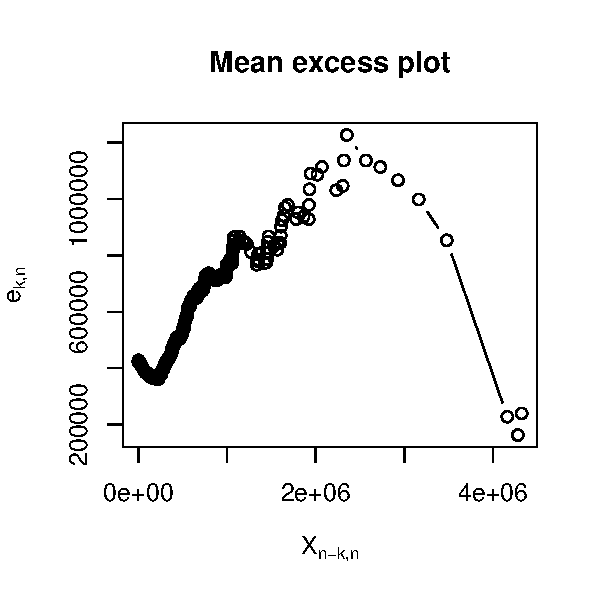
\includegraphics[width=\textwidth]{./plots/MeanExcess.pdf}
	\end{subfigure}
		\begin{subfigure}[t]{0.45\textwidth}
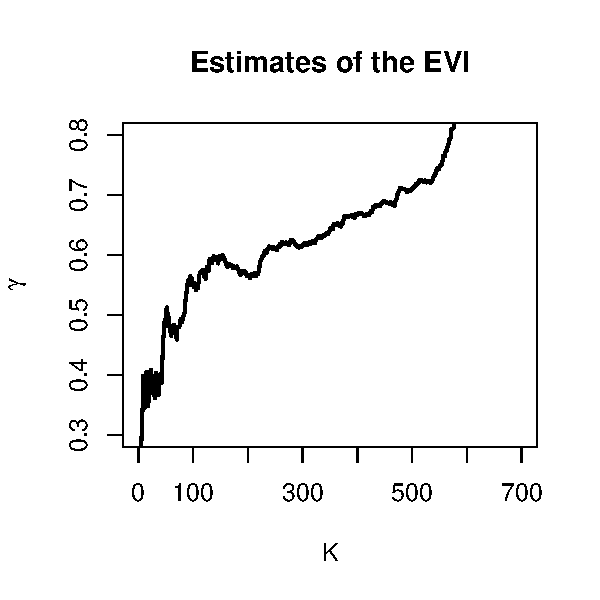
\includegraphics[width=\textwidth]{./plots/HillGPD.pdf}
	\end{subfigure}
	\caption{Mean Excess (left) and Hill estimates of the EVI (right) of the ultimates}
	\label{fig_hillgpd}
\end{figure}
It can be seen from Figure \ref{fig_hillgpd} (right) that the $e_{k,n}$ increases with increasing $X_{n-k,n}$, indicating that the tail of the ultimates data is heavier than exponential and thus validating the use of an estimator of a positive $\gamma$ such as the Hill estimator. Figure \ref{fig_hillgpd} (right) shows a plot of the Hill estimates for the ultimates data as a function of the $k$ (number of observations above the threshold). The plot has no apparent form of stability. This problem is very common in practice where the Hill estimator is volatile and hard to interpret and hence commonly referred to as the \textbf{``Hill horror plot''}. Although there are numerous methods to aid a practitioner in making a suitable choice of the right value of $k$. This choice however is to some degree, subjective. This is further discussed in Section {\ref{thresholdsection}}.

\subsubsection*{Censored data}
One of many difficulties related to tail estimation in EVT is modelling data that is subject to random right censorship. This problem is very common in areas such as reinsurance and survival analysis in clinical trials. 

\textbf{Clinical trials}: suppose for example a study is conducted to see how long patients can survive when placed on a certain drug. At the end of the study, some of these patients may still be alive. This is an example of right censoring. The quantity in question (time to death) is not fully observable. \cite{gomes2011estimation} conducted such a case study to survival data sets.

\textbf{Insurance}: here we can revisit the MTPL data studied in \autoref{mtplsection}. We have discussed the ultimate loss projections made by experts. This data set also contains indexed total incurred values as well as the indexed total paid values.

Figure \ref{mtpl_fourclaims} \footnote{Figure \ref{mtpl_fourclaims} is taken from \cite{albrecher2017reinsurance} with authorisation from the authors} illustrates the development of four claims occurring 1995, 1996, 1997 and 1998. The full line indicates the cumulative indexed payment, while the dashed lines indicates the indexed incurred values. 

The incurred values at a particular point in time are the sum of the already paid amounts and the amounts reserved as estimated by experts. When the two lines meet i.e. the cumulative payment and the incurred value are equal, and the claim is closed. 

This happens in the first and third claim while the second and fourth claim appear to still be in development. These two claims (second and fourth claim) are thus right censored at the time of evaluation (end of 2010). 

\begin{figure}[t]
\centering
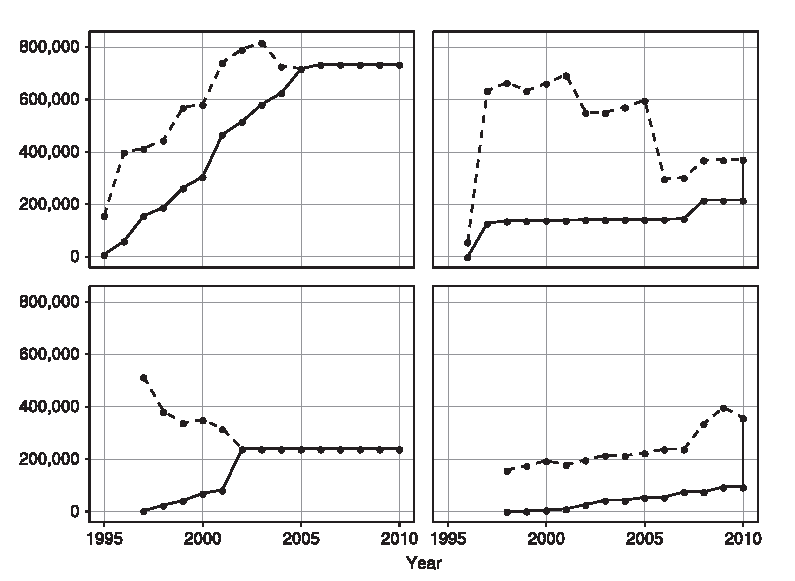
\includegraphics[width=\textwidth]{./plots/mtpl_claims.pdf}
\caption{Development patterns for four particular claims }

\label{mtpl_fourclaims}
\end{figure}
%Figure \ref{mtpl_iti} and Figure \ref{mtpl_itp} shows the indexed total incurred values and total paid values %respectively. As can be expected, most claims occurring closer to 2010 are not developed at the time of %evaluation. 
There will be an inevitable amount of uncertainty in the approximation of ultimate loss projections. Instead of relying on these ultimate loss projections when modelling tail behaviour we can adopt a right censoring framework and only use the indexed total payments at the end of the evaluation year as lower bounds.

Consider $X =\text{\it index total incurred}$ and $C =\text{\it indexed total paid}$. 
We shall work with observations $Z = \min(X,C)$.
\begin{itemize}
\item If a claim is closed at portfolio evaluation then $Z=X$ is observable and the censoring indicator $\Delta = 1$;
\item If a claim is still under development at portfolio evaluation then $Z=C$, thus not completely observable and the censoring indicator $\Delta = 0$;
\end{itemize}Therefore $Z\leq X$ and we use the ordered sample $\{Z_{i,n},\Delta_{i,n},\ i=1,...,n\}$.
This case study is conducted with more detail in \autoref{chap4::Sec6}.
%\begin{figure}[h]
%\centering
%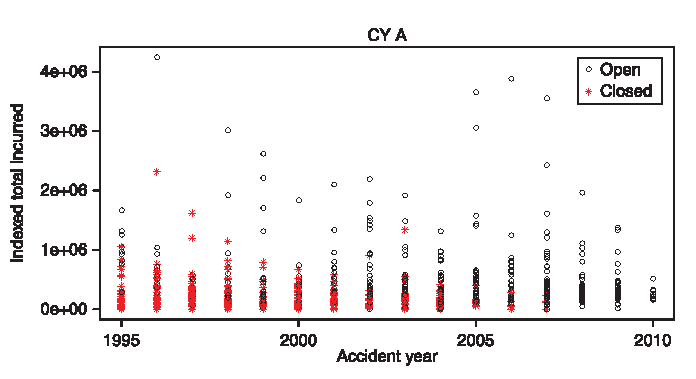
\includegraphics[width=0.95\textwidth]{./plots/ITI.pdf}
%\caption{Company A: incurred losses}
%\label{mtpl_iti}
%\end{figure}

%\begin{figure}[h]
%\centering
%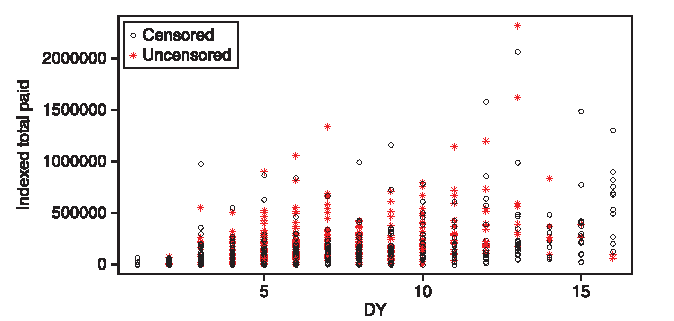
\includegraphics[width=\textwidth]{./plots/ITP.pdf}
%\caption{Company A: incurred losses}
%\label{mtpl_itp}
%\end{figure}

Over the last couple of years, EVT under random right censoring has received considerable attention in literature. A good overview of the subject was made by \cite{beirlant2001pareto} who proposed adapting the Hill estimator under random right censorship.
\\\\
Under some conditions \cite{delafosse2002almost} were able to prove almost sure convergence of this adapted Hill estimator under random right censorship. The authors \cite*{reiss2007statistical} proposed a POT framework by adapting the likelihood function of the distribution of excesses above a threshold. However, the authors did not study the asymptotic properties of the proposed estimators.
\\\\
\cite{beirlant2007estimation} proposed a different approach, generalisation of the POT methodology using the GPD. They also proposed an adaptation of the moment estimator developed by \cite{dekkers1989moment}.
\\\\
\cite{einmahl2008statistics} considered a general adaptation of various estimators of the EVI under random censorship. Under some restrictive conditions, the authors proved the asymptotic normality result of the estimators in detail. \cite{brahimi2015gaussian} proved the asymptotic normality result of the adapted Hill estimator under more relaxed conditions.
\\\\
\cite{gomes2011estimation} provided a good overview of the EVI estimators under random censoring and proposed an adapted minimum-variance reduced-bias (MVRB) estimator \citep{caeiro2005direct}. Using samples from models in the Fréchet domain the authors conducted a simulation study which demonstrated the overall best performance of their adapted MVRB estimator.
\\\\
\cite{worms2014new} presented a methodological paper for the estimation of the EVI under random right censorship, based on the ideas of Kaplan-Meier integration and the synthetic data approach of \cite{sue1987linear}. We show in this thesis how to reinterpret their approach using the mean excess function. Under mild censoring, the authors were able to prove consistency of the proposed estimators.
\\\\
\cite{ameraoui2016bayesian} proposed a Bayesian method to estimate the EVI under random right censoring by developing maximum a posteriori and mean posterior estimators using the Maximal Data Information (MDI), Jeffreys and the conjugate Gamma priors. The authors also establish consistency and asymptotic normality of the proposed estimators.
\\\\
In this thesis a bias reduced version of the \cite{worms2014new} estimator is proposed in \autoref{chap4}, and the idea of shrinkage introduced in \autoref{chap3} is further applied to the proposed estimator. \cite{beirlant2018estimation} study the asymptotic and finite sample behaviour of the large class of estimators first proposed in \cite{worms2014new}, paying special attention to heavy censoring.
\\\\
\subsection{Threshold selection}\label{thresholdsection}
An important question in practical applications of statistics of extremes is the threshold choice. There exists a number of methods available for practitioners to aid in choosing a suitable threshold. The threshold selection problem is however still an open research question. The threshold selection problem is a bias-variance trade off problem \citep{coles2001introduction}. By counterpoint, if the threshold is too high it will lead to fewer excesses to estimate the parameters and will thus lead to a high variance. However if the threshold is too low, the asymptotic motivation of the underlying POT model no longer holds and thus a large bias will be present.
\\\\
The fixed threshold approach is very common in EVT tail estimation. In this approach, the threshold is chosen prior to model fitting. The threshold choice is hereon interchangeably mentioned as; the threshold value from which to consider the data as extremes or the choice of the number ($k$) of upper extremes. 
\\\\
\cite{dumouchel1983estimating} proposed a simple quantity based rule of thumb to consider the top 10\% largest observations as the tail fraction. \cite{loretan1994testing} proposed a data driven approach to choose $k=\dfrac{n^{2/3}}{\log[\log(n)]}$. \cite{ferreira2003optimising} proposed to choose the tail fraction as $k=\sqrt{n}$ through simulation studies. 
\\\\
\cite{hall}, \cite{dekkers1993optimal} and \cite{de1998comparison} proposed choosing a $k$ that minimizes the asymptotic MSE of any proposed estimator. \cite{beirlant1999tail} introduced a heuristically motivated procedure by directly estimating the asymptotic mean squared error. \cite{drees1998selecting} proposed a sequential approach to selecting the optimal sample fraction. Their approach requires an arbitrary choice of a tuning parameter. \cite{draisma1999bootstrap}, \cite{gomes2001bootstrap} and \cite{danielsson2001using} used bootstrap methods to choose the optimal sample fraction. \cite{matthys2000adaptive} provide a review of several adaptive threshold selection techniques. See also Section 4.7 in \cite{sts626}.
\\\\
\cite{dupuis1999exceedances} proposes a method of threshold estimation for the GPD. The procedure assigns to each observation a weight between zero and one. A high weight indicates a good fit and thus the data point should be retained. The author suggests starting with a lower choice of the threshold and increasing it until the weights are all `close to one'. \cite{coles2001introduction} show that diagnostic plots such as the QQ plot, parameter stability plot and the mean excess plot can be used to choose the threshold. Refer to \cite{caeiro2015threshold} for a recent review on the subject of threshold selection.
\\\\
A concern with using the fixed threshold approach is that the threshold value consistent with GPD assumptions is regarded as known and extrapolation is then conducted given this known value. Thus threshold uncertainty is not naturally taken into account. Moreover, in comparing the estimation results from different thresholds, it is often found that plausible but different threshold values, lead to different EVI estimates.

\subsection{Bias reduction}
In order to address the inadequacies of threshold selection under the POT framework, the concept of bias reduction has been studied extensively. Many of these studies however are focused mainly on the $\gamma>0$ case.
\\\\
\cite{peng1998asymptotically}, \cite{caeiro2002class}, \citet{gomesa2002asymptotically,gomes2004bias} and \citet{gomes2002semi,gomes2005revisiting} proposed bias reduction methods that seek to cancel out the bias terms through an indirect approach of using weighted combinations of different estimators.
\\\\
\citet{beirlant1999tail, beirlant2008improved}, \citet{feuerverger1999estimating} and \citet{gomes2000alternatives,gomes2007improving} proposed bias reduction methods based on scaled log-spacings between subsequent high order statistics from a Pareto-type distribution.
\\\\
\cite{caeiro2005direct} proposed minimum variance reduced bias estimators of the EVI, where the bias is reduced without increasing the variance with respect to the Hill estimator. This method is based on adequate external estimation of a pair of parameters of second order slow variation under a third order condition which we do not discuss in this thesis. Following this work, proposals by \cite{gomes2007sturdy,ivette2007simple}, \cite{gomes2008tail} and \citet{caeiro2008minimum} consider directly subtracting the bias term as given by the asymptotic distribution.
\\\\
\cite{beirlant2009second} proposed a much more flexible model adequately capturing the deviation between the true excess right tail function and the asymptotic Pareto model. This approach substantially reduced bias by considering the Hall-class of Pareto-type models in (\ref{hall}). This approach often leads to much improved results, both in bias and MSE.

\\
\subsection{Mixture modelling in EVT}
The main motivation behind use of mixture models in EVT is to improve flexibility of tail models, which generally only focus on the tail part of the data and not the complete data set. This area of research has over the last decade gained considerable interest. \cite{frigessi2002dynamic} proposed an unsupervised tail estimation technique using a dynamic mixtures of two components with a weight function $\pi=\pi(x)$ smoothly connecting the bulk and the tail of the distribution. \cite{sts626} suggested the need for a global statistical model describing the entire range of possible claim outcomes using an exponential and a Pareto mixture.
\\
\cite{behrens2004bayesian} considered a Bayesian approach of fitting a parametric mixture model using indirect expert elicited prior distributions. This Bayesian posterior inference does however have a major draw back. Since it treats the prior on the threshold parameter and other parameters as independent, the dependence between the scale and threshold parameters is simply ignored. \cite{tancredi2006accounting} also accounts for threshold uncertainty by estimating the threshold as one of the parameters in the mixture model. 
\\
\cite{carreau2009hybrid2} proposed a hybrid Pareto model by stitching a GPD tail with a normal distribution and setting a continuity constraint on the density and its first derivative. Performance of this method is however poor in practice. Improvement and extension of the performance of this hybrid Pareto model is made by \cite{carreau2009hybrid1}.
\\
\cite{macdonald2011flexible} considered a mixture approach where the bulk of the distribution is estimated by a standard kernel density estimator. Using penultimate theory \cite{wadsworth2012likelihood} account for threshold uncertainty and provide a likelihood ratio testing procedure for the threshold choice.
\\\\
By applying the inverse CDF of the GPD to more richer Beta distributed draws instead of uniform draws, \cite{papastathopoulos2013extended} proposed general extensions to the GPD distribution. Following from this work, \cite{naveau2016modeling} proposed a version of the extended statistical model called the extended generalised Pareto distribution (EGPD) which is in compliance with EVT and allows for a smooth transition between the modal and tail part of the data. Building further from this work, \cite{tencaliec2018flexible} proposed a flexible semiparametric GP modelling approach by estimating the key component of the EGPD class in \cite{naveau2016modeling} using Bernstein polynomials.

\section{Data sets and Software}
In this section, we give a description of all the data sets used in this thesis for practical illustrations. A description of the software used to conduct simulation studies is also given.

\begin{enumerate}
\item \textbf{Secura Belgian Re data}\\
The Secura Belgian Re is studied in \autoref{chap3} as first studied by \cite{sts626}. The data set contains 371 automobile claims larger than or equal to 1,200,000 Euros for the year 1988 to 2001, collected from various insurance companies in Europe. All amounts have been indexed.
\item \textbf{Motor third-party liability (MTPL) data}\\
Details of this data are given in \autoref{mtplsection}. The data set is further studied in \autoref{chap4}.
\item \textbf{Mont-Aigoual station rainfall data}\\
This rain fall data is studied in \autoref{chap5}. The data set was first studied by \cite{carreau2017partitioning} and \cite{tencaliec2018flexible}. It contains daily precipitation of all seasons from the year 1976 to 2015 recorded at the Mont-Aigoual station, south of France.
\end{enumerate}

\subsection*{Software}
All simulations in this thesis were conducted using the \textbf{R} \citep{R} software through a Linux based high performance computing unit. The simulation study conducted in \autoref{chap5} are more extensive and thus resulted in large output data files. To avoid making too many plots, an interactive web application is build using an \textbf{R} package called shiny \citep{shiny} and hosted as a standalone application on the following url: \url{https://phdshinygao.shinyapps.io/ExtendedModels/}. Guidelines regarding usage of the interactive web application are given in Appendix \ref{shiny}.

\section{Chapter conclusion}
In this chapter, an overview of EVT has been given, along with a review of literature leading up to proposals made in this thesis. A motivating data set was used to give a short illustration of the need for EVT, moreover discuss a growing research interest of an EVT framework for dealing with censored extremes. Finally, descriptions of all the data sets and software used in this thesis were given.
\\\\
The next chapter marks the beginning of \autoref{part1} of the thesis which will introduce the method of shrinkage estimation in \autoref{chap3} and propose a bias reduced estimator of the EVI in \autoref{chap4}. \autoref{chap5} in \autoref{part2} of the thesis will propose a novel bias reduction technique in all domains of attraction and an overall conclusion will be made in \autoref{chap6}.

\part{Second-order Refinements: Heavy Tails ($\gamma>0$)}\label{part1}
\chapter{Using Shrinkage Estimators to Reduce Bias and MSE in Estimation of Heavy Tails}\label{chap3}
\setcounter{equation}{0}

\href{https://www.ine.pt/revstat/pdf/Usingshrinkageestimatorstoreducebias.pdf}{\textit{This chapter is based on Beirlant, J., Maribe, G. and Verster, A., 2019. Using shrinkage estimators to reduce bias and MSE in estimation of heavy tails. REVSTAT–Statistical Journal, 17(1), pp.91-108.}}

\section{INTRODUCTION} % --- sections in UPPERCASE
\label{paper1:sec1}       % --- this section label
In this section we consider the estimation of the EVI $\gamma$ and tail probabilities $P(X>x)$ for $x$ large, on the basis of independent and identically distributed observations $X_1, X_2, \ldots, X_n$ which follow a Pareto-type distribution with right tail function (RTF) given by
\begin{equation}
\bar{F}(x) = 1-F(x) = P(X>x) = x^{-1/\gamma} \ell (x)
\label{Patype1}
\end{equation}
where $\ell$ is a slowly varying function at infinity, {\it i.e.}
$$
{\ell (ty) \over \ell (t)} \to 1, \mbox{ as } t \to \infty, \mbox{ for every } y>1.
$$
The most famous estimator of $\gamma$ was first derived by \cite{hill1975simple} as a ML estimator approximating the RTF of the excesses ${X \over t} |X>t$ over a large threshold $t$ by a simple Pareto distribution with RTF $y^{-1/\gamma}$: 
\begin{equation}
\bar{F}(ty)/\bar{F}(t) \approx y^{-1/\gamma}, t \mbox{ large}.
\label{Pot}
\end{equation}
When setting $t= X_{n-k,n}$ where $X_{1,n}\leq X_{2,n} \leq \ldots \leq X_{n,n}$ the ML estimator is given by
\begin{equation}
H_{k,n} = {1 \over k}\sum_{j=1}^k \log {X_{n-j+1,n} \over X_{n-k,n}}.
\label{Hill}
\end{equation}
A simple estimator of a tail probability $P(X>x)$ with $x$ large, introduced in Weissman (1978), is then obtained from \eqref{Pot} setting $ty = x$ and estimating $P(X>t)$ by the empirical proportion $k/n$: 
\begin{equation}
\hat{p}_{x,k} = {k \over n}\left( {x \over X_{n-k,n}}\right)^{-1/H_{k,n}}.
\label{Weiss}
\end{equation}
In practice, a way to verify the validity of model \eqref{Patype1} is to check whether the Hill estimates are stable as a function of $k$. However in most cases the stability is not visible, which can be explained by slow convergence in \eqref{Pot}. For this reason bias reduced estimators have been proposed which lead to plots that are much more horizontal in $k$ which facilitates the analysis of a practical case to a great extent.

\cite{beirlant2009second} proposed a more flexible model capable of capturing the deviation between the true excess RTF $\bar{F}(ty)/\bar{F}(t)$ and the asymptotic Pareto model. For a heavy tailed distribution \eqref{Patype1}, this deviation can be parametrized using a power series expansion \citep{hall}, or more generally via second-order slow variation \citep{bingham1987regular}. 
More specifically in \cite{beirlant2009second} the subclass $\mathcal{F}(\gamma,\tau)$ of the Pareto-type tails \eqref{Patype1} was considered satisfying
\begin{eqnarray}
\bar{F}(x) = C x^{-1/\gamma}\left( 1+\gamma^{-1}\delta (x)\right),
\label{Sclass}
\end{eqnarray}
with $\delta (x)$ eventually nonzero and of constant sign such that $|\delta(x)|=x^\tau \ell_{\delta}(x)$ with $\tau <0$ and $\ell_{\delta}$ slowly varying. 
It was shown that under $\mathcal{F}(\gamma,\tau)$ as $t \to \infty$
$$
\sup_{y \geq 1}\left|{\bar{F}(ty)\over \bar{F}(t)} - \bar{G}_{\gamma,\delta,\tau}(y) \right|
= o\left(|\delta (t)| \right)
$$
with $\bar{G}_{\gamma,\delta,\tau}$ the RTF of the EPD
\begin{equation}
\bar{G}_{\gamma,\delta,\tau}(y)=\{y(1+\delta-\delta y^{\tau})\}^{-1/\gamma}, \ \ \ y>1,
\label{EPD}
\end{equation}
with $\tau <0 < \gamma$ and $\delta > \max (-1,1/\tau)$.
This shows that the EPD improves the approximation \eqref{Pot} with an order of magnitude.
Then ML estimation of the parameters ($\gamma,\delta$) based on a set of excesses 
$\left(Y_{j,k}:=X_{n-j+1,n}/X_{n-k,n},\; j=1,\ldots,k \right)$ was used to obtain a bias reduced estimator $\hat{\gamma}^{ML}_{k,n}$ of $\gamma$. Bias reduction of the Weissman estimator of tail probabilities can analogously be obtained using 
\begin{equation}
\hat{p}^{EP}_{x,k} = {k \over n}\bar{G}_{\hat\gamma _k,\hat\delta _k,\hat\tau}\left( {x \over X_{n-k,n}}\right),
\label{PEP}
\end{equation}
where $(\hat\gamma _k,\hat\delta _k)$ denote the ML estimators based on the EPD model, and where $\hat\tau$ is a consistent estimator of $\tau$, to be specified below, which was shown not to affect the asymptotic distribution of $(\gamma,\delta)$.
\\\\
If $F$ satisfies $\mathcal{F}(\gamma,\tau)$, it is shown in \cite{beirlant2009second} that $U(x):= Q(1-x^{-1})$ ($x>1$), with 
$Q(p) = \inf \{x: F(x) \geq p \}$ ($p \in (0,1)$), satisfies
\begin{equation}
U(x) = C_a{\gamma} x^{\gamma}\left(1+ a(x) \right)
\label{Q}
\end{equation}
with $a(x) = \delta (Q(1-x^{-1}))\{1+o(1)\}= \delta (C_a{\gamma} x^{\gamma})\{1+o(1)\}$ as $x \to \infty$. In particular
$a$ is eventually nonzero and of constant sign and $|a(x)|= x^{\rho}\ell_{a}(x)$ with $\ell_a$ slowly varying and $\rho=\gamma\tau$. Here we assume $|\ell_a (x)|= C_a (1+o(1))$ as $x \to \infty$ for some constant $C_a>0$.
\\\\
The following asymptotic results have been derived for $H_{k,n}$ and $\hat{\gamma}^{ML}_{k,n}$ assuming that $F$ satisfies $\mathcal{F}(\gamma,\tau)$, and $\sqrt{k} a(n/k) \to \lambda \in \mathbb{R}$ and $\hat{\rho}_{k,n} = \rho + o_p(1)$ as $k,n \to \infty$ and $k/n \to 0$, the following asymptotic results hold for the EPD-ML estimator $\hat{\gamma}^{ML}_{k,n}$ and $H_{k,n}$:
\begin{eqnarray}
\sqrt{k} \left( H_{k,n}-\gamma \right) & \to^d & 
\mathcal{N}\left(\lambda {\rho \over 1-\rho} , \gamma^2
\right), \label{limH} \\ 
\sqrt{k} \left( \hat{\gamma}^{ML}_{k,n}-\gamma \right) & \to^d & 
\mathcal{N}\left(0, \gamma^2 \left({1-\rho \over \rho} \right)^2
\right).
\label{limML} 
\end{eqnarray}
An estimator $\hat{\rho}_{k,n}$ of $\rho$ can be taken from \cite{alves2003new} using $k=k_1= \lfloor n^{1-\epsilon}\rfloor$ for some $\epsilon >0$ (see, Appendix \ref{appendix1b}). The required consistency for $\hat{\rho}_{k,n}$ was obtained under \eqref{Q}.
\\\\
Asymptotic results of the type \eqref{limH} and \eqref{limML} are typical for bias reduced estimators when both $\gamma$ and $a(n/k)$ or $\delta$ are jointly estimated at every $k$ value:
for larger values of $k$ corresponding to $\sqrt{k} a(n/k) \to \lambda \neq 0$, bias reduced estimators still have asymptotic bias 0 in contrast to the Hill estimator, but their variance is increased by a factor $((1-\rho)/\rho)^2$ compared to $H_{k,n}$.
\\\\
In a pioneering paper, \cite{caeiro2005direct} proposed to estimate $(n/k)^{-\rho} a(n/k)$ at a high level $k=k_1= \lfloor n^{1-\epsilon}\rfloor$, leading to a corrected Hill estimator (denoted below by $CH_{k,n}$) with asymptotic variance $\gamma^2$ and excellent bias and MSE characteristics. To obtain the normal asymptotic behaviour of such minimum variance reduced bias estimators one needs a third-order slow variation condition which is more restrictive than \eqref{Q} or condition $\mathcal{F}(\gamma,\tau)$.  

\vspace{0.3cm}\noindent
Up to now, to the best of our knowledge, the fact that $\delta (t) \to 0$ as $t \to \infty$, or $a(n/k)\to 0$ as $n/k \to \infty$ has not been exploited in the literature. However, this calls for shrinkage estimators.
Such shrinkage approach can be implemented by putting a penalty on $\delta$ in an ML procedure, leading to penalised ML. Alternatively a penalty on $\delta$ can be naturally introduced in a Bayesian approach putting an appropriate prior on this parameter. 
\\\\
Here we investigate the use of shrinkage estimation when modelling the distribution of the vector of excesses ${\bf Y}_k := \left( Y_{j,k}, j=1,\ldots,k \right)$
with an EPD. In \autoref{chap3::sec2} we show that a quadratic penalty, or equivalently a normal prior, on $\delta$ with zero mean and variance $\sigma^2_{k,n}$, depending in an appropriate way on $k$ and $n$, leads to interesting asymptotic MSE results for $\gamma$. In \autoref{chap3::simulation} we 
consider the finite sample behaviour of the penalised likelihood and Bayes approach, and make a comparison with the minimum variance reduced bias estimator, and consider a practical case. 

\section{Shrinkage estimators of the EPD parameters}\label{chap3::sec2}

\subsection{penalised likelihood and Bayesian interpretation}
ML estimation of the EPD parameters ($\gamma,\delta$), given a value of $\tau$, follows by maximising the log-likelihood
\begin{eqnarray}
{1 \over k}l_{EP}(\gamma,\delta |{\bf y}) &=& -\log \gamma
-(\frac{1}{\gamma}+1){1 \over k}\sum_{j=1}^k\left[\log y_{j,k} + \log(1+\delta\{1-y_{j,k}^{\tau}\})\right] \nonumber \\&&
+{1 \over k}\sum_{j=1}^k\log\left(1+\delta\{1-(1+\tau)y_{j,k}^{\tau}\}\right).
\label{logl}
\end{eqnarray}
Shrinkage estimators are then obtained by putting a penalty on $\delta$. Below it will be shown that a quadratic penalty is appropriate in view of the asymptotic results for the penalised maximum likelihood (PML) estimators $(\hat{\gamma}_{k,n}^{P},\hat{\delta}^P_{k,n})$. These estimators are then obtained by optimising the log-likelihood
\begin{equation}
{1 \over k}l_{pen} (\gamma,\delta |{\bf y}) = {1 \over k}l_{EP}(\gamma,\delta |{\bf y}) - \omega {\delta^2 \over 2k\sigma_{k,n}^2}, 
\label{loglp}
\end{equation}
where $\omega >0$ serves as a tuning constant regulating the amount of penalty, and $\sigma_{k,n}^2$ indicating the penalty rate as a function of $k$. From the asymptotic analysis below, it follows that $\sigma^2_{k,n} = (k/n)^{-2\rho}$ is appropriate. 
\\\\
Alternatively, from a Bayesian perspective, a shrinkage estimator is obtained by considering the posterior mode estimators $(\hat{\gamma}_k^{B},\hat{\delta}_k^B)$ of the log-posterior
\begin{equation}
{1 \over k} \log p (\gamma,\delta|{\bf y}) = 
{1 \over k}l_{EP}(\gamma,\delta |{\bf y}) + {1 \over k}\log \pi (\gamma,\delta),
\label{logpost}
\end{equation}
where $\pi (\gamma,\delta)$ denotes the prior density on $(\gamma,\delta)$. In correspondence with the choice for the penalised log-likelihood \eqref{loglp}, we here choose a normal prior on $\delta$ with mean 0 and variance $\sigma^2_{k,n}$. We also truncate it from the left in order to comply with the restriction
$\delta > \max (-1,1/\tau)$:
\begin{equation}
\pi (\delta) = {1 \over \sqrt{2\pi}\sigma_{k,n}}e^{-{1 \over 2}{\delta^2 \over \sigma^2_{k,n}}}/ \left( 1-\Phi (\max (-1,\tau^{-1})/\sigma_{k,n})\right).
\label{pidelta}
\end{equation} 

\subsection{Asymptotic results for the penalised ML estimator $\hat{\gamma}^P_k$}

In Appendix \ref{appendix1} we derive that the first order approximations ($\gammab,\db$) of the penalised ML estimators are given by
\begin{eqnarray*}
	\gammab & =& H_{k,n} +\db \left( 1-E_{k,n}(\tau) \right) ,\\
	\db &=& \frac{1-H_{k,n}\tau}{D^{P}_{k,n}} \left(E_{k,n}(\tau) - {1 \over H_{k,n}\tau} \right)
\end{eqnarray*}
where 
$$
E_{k,n}(s) = {1 \over k}\sum_{j=1}^k Y_{j,k}^{s},\; s < 0,
$$
and 
\begin{eqnarray*}
D^{P}_{k,n} =
{\omega \gammab \over k\sigma^2_{k,n}} -
 \Big(1 &-& 2(1-\gammab \tau) E_{k,n}(\tau)+ (1-2\gammab\tau-\gammab\tau^2)E_{k,n}(2\tau) \\ 
&-& \tau (1- E_{k,n}(\tau))E_{k,n}(\tau)\Big).
\end{eqnarray*}
These expressions are identical to the asymptotic EPD-ML estimators derived in \cite{beirlant2009second} except for the extra term ${\omega \gammab\over k\sigma^2_{k,n}}$ in the expression of $D^{P}_{k,n}$. 
As an external estimator of $\tau$ we use $\hat{\tau} = \hat{\rho}_{k,n}/H_{k,n}$ with $\hat{\rho}_{k,n}$ taken from \cite{alves2003new}. Moreover we set $\zeta=\gamma^2 (1-2\rho)(1-\rho)^2$. The following result is derived in Appendix \ref{appendix1}. 
\\
\begin{theorem}\label{theorem11} {\it Let $F \in \mathcal{F}(\gamma,\tau)$ with $|a(x)| =x^{\rho }C_a (1+o(1))$ as $x \to \infty$. Assume that $\sqrt{k} a(n/k) \to \lambda$ as $k,n \to \infty$, $k/n \to 0$. Setting $\sigma_{k,n}^2= (k/n)^{-2\rho}$, it follows that $\gamma_{k,n}:=\sqrt{k} \left( \gammab-\gamma \right)$ is asymptotically normal with asymptotic mean and variance given by
	\begin{eqnarray}
	E_{\infty} (\gamma_{k,n}) &=& 
	{\lambda \rho \over 1-\rho}{\zeta C_a^2 \omega \over \zeta C_a^2 \omega + \rho^4 \lambda^2}, 
	\label{Abias}\\
	Var_{\infty} (\gamma_{k,n})&=& {\gamma^2 \rho^8\lambda^4 \over (\rho^4\lambda^2+ \zeta C_a^2 \omega )^2}\left( \left({1-\rho \over \rho} \right)^2
	+ {\zeta^2 C_a^4 \omega^2 \over \rho^8 \lambda^4}+ 2{\zeta C_a^2 \omega \over \rho^4 \lambda^2}\right). 
	\label{Avar}
	\end{eqnarray}
	$\blacktriangle$
}
\end{theorem}

\vspace{0.3cm}\noindent
Minimising $MSE_{\infty}(\gamma_{k,n})= E^2_{\infty} (\gamma_{k,n})
+ Var_{\infty} (\gamma_{k,n})$ 
with respect to $\omega$, this leads to the asymptotically optimal value (see Appendix \ref{appendix1a}) $$\omega_{opt}= C_a^{-2}.$$ 
One then obtains from \eqref{Abias} and \eqref{Avar} that 
\begin{eqnarray*}
	E^{opt}_{\infty} (\gamma_{k,n}) &=& {\lambda \rho\over 1-\rho}
	{\zeta \over \zeta + \lambda^2 \rho^4 },\\
	Var^{opt}_{\infty} (\gamma_{k,n}) &=& {\gamma^2 \over (\lambda^2\rho^4+ \zeta)^2}
	\left\{(1-\rho)^2\rho^6 \lambda^4 + \zeta^2 + 2\zeta \rho^4\lambda^2 \right\},
\end{eqnarray*}
from which 
\begin{equation}
MSE^{opt}_{\infty}(\gamma_{k,n}) =
\gamma^2 + { \lambda^2 \rho^2 \gamma^2 (1-2\rho) \over \gamma^2 (1-2\rho)(1-\rho)^2 + \rho^4 \lambda^2}.
\label{xisqdiff}
\end{equation}
Since the right hand side of \eqref{xisqdiff} is an increasing function in $\lambda^2$ it follows that
$$
MSE^{opt}_{\infty}(\gamma_{k,n}) \leq \lim_{\lambda \to \infty}MSE^{opt}_{\infty}(\gamma_{k,n}) = MSE_{\infty}\left(\sqrt{k}(\hat{\gamma}_{k,n}^{ML}-\gamma)\right)= \gamma^2 ({1-\rho \over \rho})^2.
$$ 
Also, expanding the right hand side of \eqref{xisqdiff} for $\lambda^2 \to 0$ leads to 
$$
MSE^{opt}_{\infty}(\gamma_{k,n}) = \gamma^2 + \lambda^2 {\rho^2 \over (1-\rho)^2}(1+o(1)).
$$
We can conclude that the asymptotic MSE of the optimal penalised estimator is uniformly smaller than the MSE of the EPD-ML estimator as given in \eqref{limML}, while for smaller $\lambda$ this asymptotic MSE follows the asymptotic MSE of the Hill estimator, given in \eqref{limH}, up to terms of order $\lambda^2$. Hence with the penalty $\omega /\sigma^2_{k,n}= C_a^{-2}(k/n)^{2 \rho}= a^{-2}(n/k)$ in \eqref{loglp}, the penalised ML estimator asymptotically follows the better of the two existing estimators as a function of $\lambda$ or $k$.
\\\\
Replacing ($\hat\gamma _k,\hat\delta _k$) by ($\hat\gamma ^{P}_k,\hat\delta ^{P}_k$) in $\hat{p}^{EP}_{x,k}$, it follows from the proof of Theorem 5.2 in \cite{beirlant2009second} that the resulting tail probability estimator $\hat{p}^{P}_{x,k}$ satisfies the following asymptotic result under the conditions of the Theorem: \\
when $p_n = P(X>x_n)$ satisfies $np_n/k \to 0$ and $\log(np_n)/\sqrt{k} \to 0$, then 
$${\sqrt{k} \over \log (k/(np_n))}\gamma ( {\hat{p}^{P}_{x_n,k} \over p_n}-1)$$ is asymptotically normal with the same limit distribution as in the Theorem. Hence the asymptotic MSE behaviour for the tail probability estimator has the same characteristics as the tail index estimator.
\\\\
From the simulations it will follow that the choice $\omega =1$ and the use of estimator of $\rho$ taken from \cite{alves2003new} yields good results. However, in order to alleviate the problem of choosing the number of top order statistics $k$ that are used in the estimation procedure, one can choose $\omega$ adaptively with each sample aiming for a plot of $\hat{\gamma}^P_k$ as a function of $k$ which is as horizontal as possible. Setting $\hat{\gamma}_k^P =\hat{\gamma}_k^P (\omega)$ in order to emphasise the dependence of the penalised ML estimator on $\omega$, a possible choice of $\omega$ is obtained by minimising the variance of the resulting estimators for $k=1,\ldots,n$:
\begin{equation}
\omega_{mv} = \mbox{argmin}_{\omega} s^2_n \left(\hat{\gamma}^P (\omega)\right),
\label{minvar}
\end{equation}
with $s^2_n (\hat{\gamma}^P (\omega)) = {1 \over n-1}\sum_{k=1}^n \left( \hat{\gamma}_k^P (\omega) - \bar{\hat{\gamma}}^P\right)^2$.


\section{Simulations and practical case studies}\label{chap3::simulation}

Both the Bayes maximum a posteriori probability estimator and the penalised maximum likelihood estimator are implemented in \textbf{R} using the general \textbf{optim} function with default parameters. 

\noindent We performed a simulation study, taking 1000 repetitions of samples of size $n=200, 500, 1000$ studying the finite sample behaviour of $\hat{\gamma}^P_{k,n}(\omega)$  for different distributions. The bias and root mean squared error (RMSE) are plotted as a function of $k$. 
\\\\
The following distributions are used:
\begin{itemize}
	\item 
	{\it The extreme value distribution} (EV) with
	$F(x)= \exp (-(1+\gamma x)^{-1/\gamma})$ $(1+\gamma x >0)$ taking $\gamma=0.25$ in which case $\rho=-0.25$ and $C_a=1$.
	\item
	{\it The Fr\'echet distribution} with $\bar{F}(x)= 1-\exp(-x^{-1/\gamma})$ taking $\gamma = 0.5$ in which case $\rho=-1$ and $C_a=0.25$.
	\item
	{\it The Burr distribution} with $\bar{F}(x)= (1+x)^{-4/3}$ so that $\gamma = 0.75$ and $\rho=-0.75$ and $C_a=1$.
	\item
	{\it The loggamma distribution} with $\bar{F}(x) \sim constant \times x^{-2}(\log x)^3$ so that $\gamma = 0.5$, which does not belong to the class $\mathcal{F}(\gamma,\tau)$.
\end{itemize}
First in Figures \ref{paper1:fig1}-\ref{paper1:fig4} we plotted the bias and the RMSE of the Hill estimator $H_{k}$, the EPD-ML estimator $\hat{\gamma}_{k}^{ML}$, the penalised ML estimator $\hat{\gamma}^P_{k}(1)$ with $\omega=1$, the Bayesian estimator $\hat{\gamma}^B_{k}(1)$ with $\omega=1$, and the minimum variance reduced bias estimator $CH_k$ from Caeiro {\it et al.} (2005) given by
\[
CH_k = H_{k,n}\left( 1- {\hat{\beta}_{k_1} (\hat{\rho}_{k_1}) \over 1- \hat{\rho}_{k_1}}\left({n \over k} \right)^{\hat{\rho}_{k_1}}\right),
\] 
with 
\[
\hat{\beta}_k (\rho) =
\frac{ \left({k \over n} \right)^{\rho} 
\left\{ \left({1 \over k} \sum_{j=1}^k ({j \over k})^{-\rho}\right) \left({1 \over k} \sum_{j=1}^k Z_j\right) 
-\left({1 \over k} \sum_{j=1}^k ({j \over k})^{-\rho} Z_j\right) 
\right\} }
{\left({1 \over k} \sum_{j=1}^k ({j \over k})^{-\rho} \right) \left({1 \over k} \sum_{j=1}^k ({j \over k})^{-\rho} Z_j\right) -\left({1 \over k} \sum_{j=1}^k ({j \over k})^{-2\rho} Z_j\right) },
\]
where $Z_j := j(\log X_{n-j+1,n}-\log X_{n-j,n})$ $(j=1,2,\ldots)$, and $k_1 = \lfloor n^{0.99}\rfloor$. 

\noindent In Figure \ref{paper1:fig5} we briefly report on the effect of the choice of $\omega$ using $\omega=1$ and $\omega= \omega_{mv}$ and compare these with the optimal asymptotic RMSE expression from \eqref{xisqdiff}.

\noindent We conclude from the simulations that the finite sample behaviour of the proposed estimators follows the characteristics predicted by the asymptotic analysis to a great extent: for small $k$ the shrinkage estimators
$\gamma_{k}^P$ and $\gamma_{k}^B$ show a similar behaviour as the Hill estimator, while for larger $k$ the proposed estimators tend to follow the characteristics of the bias reduced EPD-ML estimator. In between these two $k$-regions the shrinkage estimators make a transition from the EPD-ML to the Hill RMSE curve. Only in the Fréchet case the Hill estimator shows a smaller RMSE than the shrinkage estimators for small $k$, while the shrinkage estimators then still show a much smaller RMSE than the EPD-ML estimator. \\\\ The Bayesian implementation shows a smaller RMSE than the penalised ML estimator, except for the Fr\'echet distribution where both RMSEs are comparable. In the latter case $\hat{\gamma}^B_k$ shows a negative bias. Also note that the difference between both the Bayesian and penalised likelihood implementation decreases as $n$ increases. \\\\ 
The results in case of the loggamma distribution are quite good. Hence it appears that the proposed method exhibits some robustness against deviations from the underlying model.
\\\\
When the plots of the shrinkage estimators are not systematically increasing with increasing $k$ as in the case of the Fr\'echet and the Burr distribution, it is useful to use the choice $\omega=\omega_{mv}$ when using the penalised ML estimator. In the case of the Fr\'echet distribution with $\omega_{opt}=16$, this adaptive choice of $\omega$ leads to a clear RMSE improvement in the transition zone (in $k$) between the Hill and EPD-ML RMSE behaviour (see Figure \ref{paper1:fig5}, top). In the Burr case (see Figure \ref{paper1:fig5}, bottom) where $C_a=1$ and hence $\omega_{opt}=1$ the choice $\omega=1$ is best, but the adaptive minimum variance choice $\omega=\omega_{mv}$ is almost as good in RMSE behaviour. 
\\\\
Overall, the proposed shrinkage estimators are competitive with respect to the minimum variance reduced bias estimator $CH_k$.
	\begin{figure}[h]
		\centering
		\begin{subfigure}[h]{0.40\linewidth}
			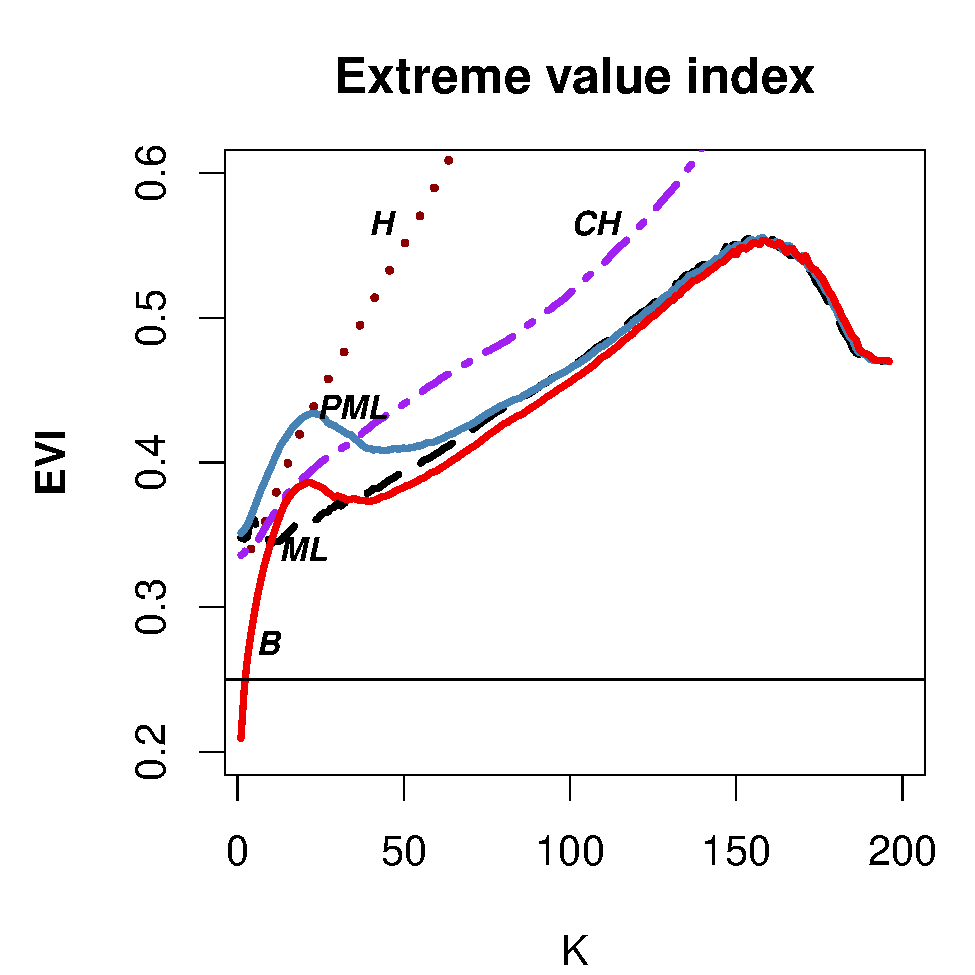
\includegraphics[width=\textwidth]{./plots/paper1/EVI_OutputGEV0,25200.pdf}
		\end{subfigure}
		\hspace{\fill}
		\begin{subfigure}[h]{0.40\linewidth}
			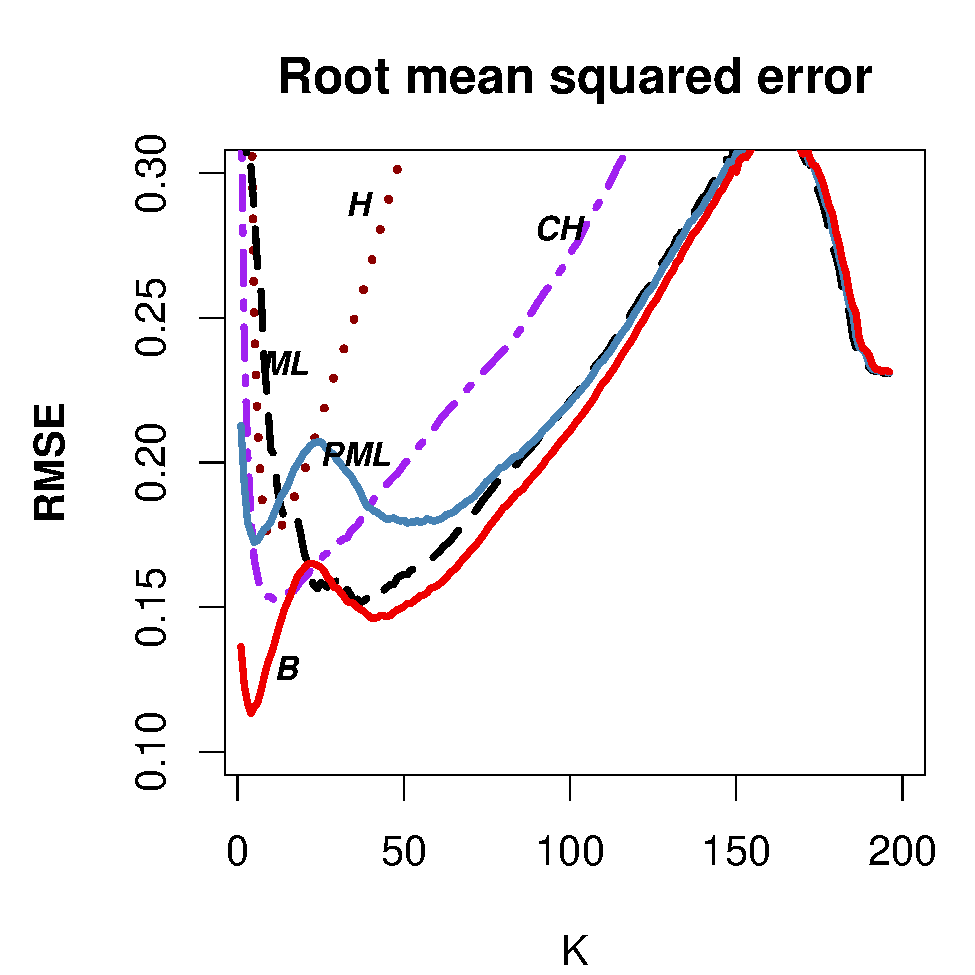
\includegraphics[width=\textwidth]{./plots/paper1/RMSE_OutputGEV0,25200.pdf}
		\end{subfigure}
		\bigskip
		\centering
		\begin{subfigure}[h]{0.40\linewidth}
			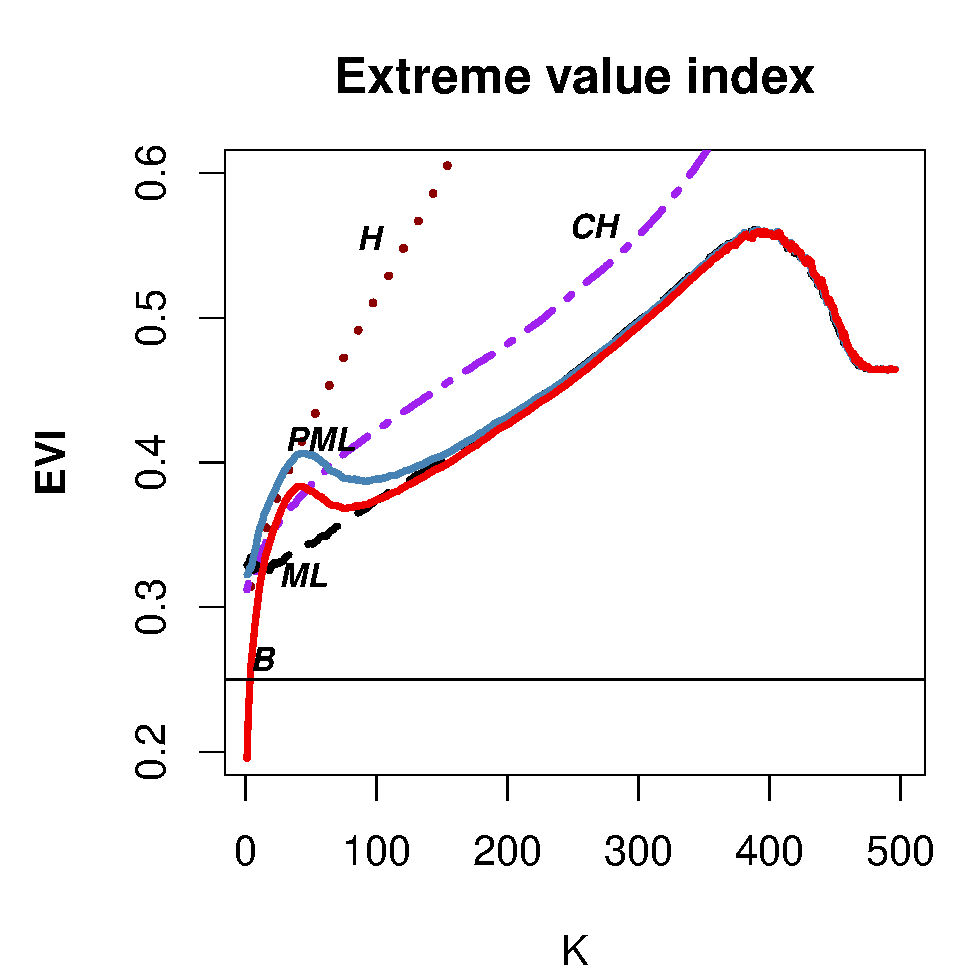
\includegraphics[width=\textwidth]{./plots/paper1/EVI_OutputGEV0,25500.pdf}
		\end{subfigure}
		\hspace{\fill}
		\begin{subfigure}[h]{0.40\linewidth}
			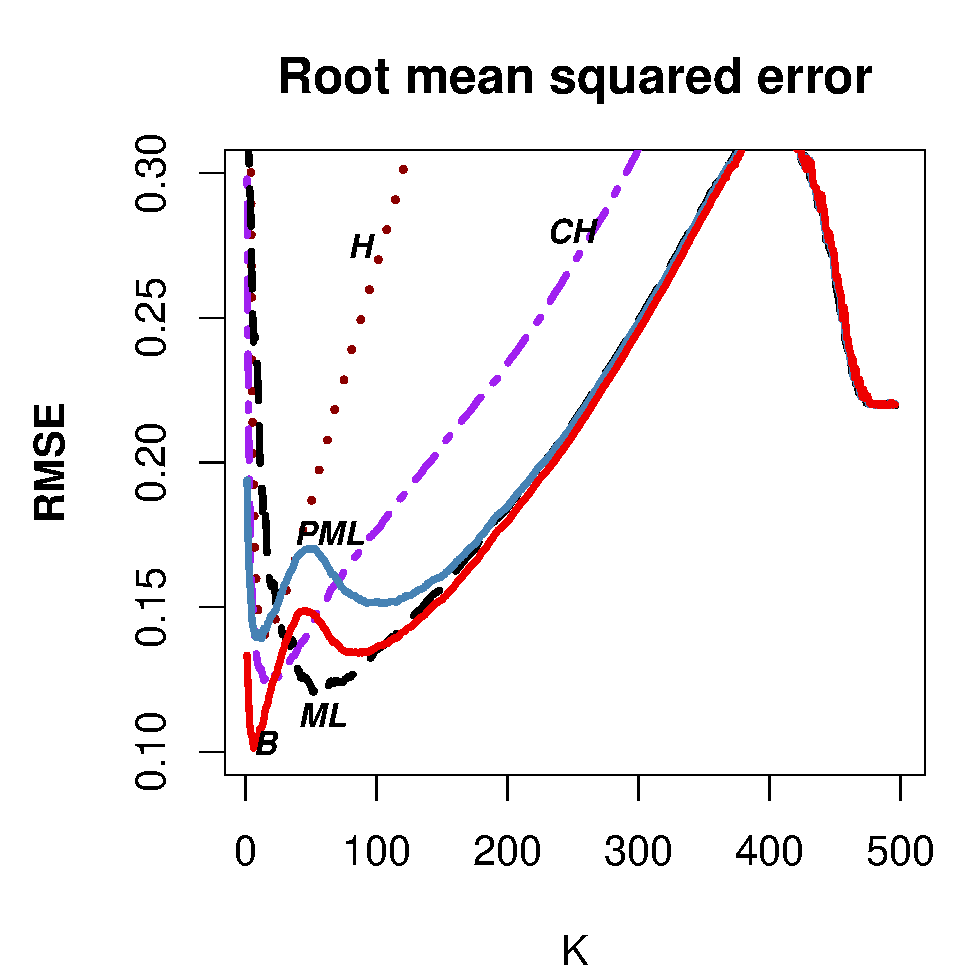
\includegraphics[width=\textwidth]{./plots/paper1/RMSE_OutputGEV0,25500.pdf}
		\end{subfigure}
		\bigskip
		\centering
		\begin{subfigure}[h]{0.40\linewidth}
			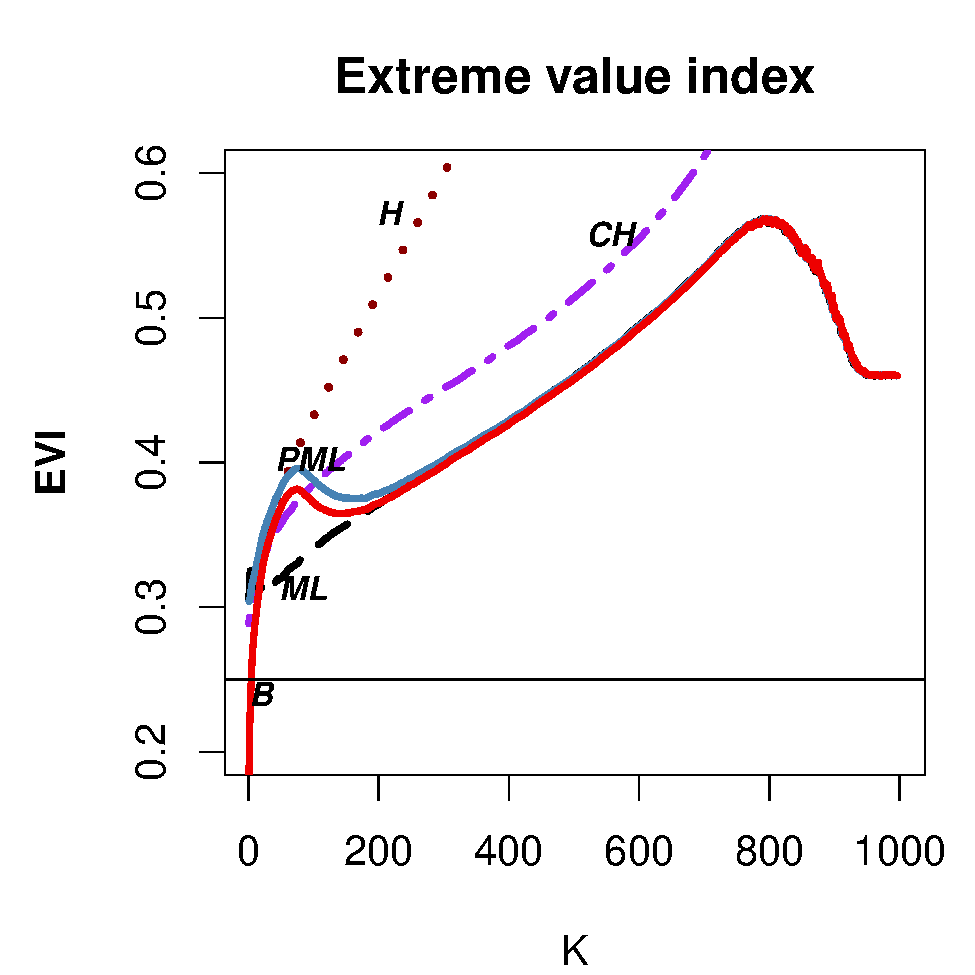
\includegraphics[width=\textwidth]{./plots/paper1/EVI_OutputGEV0,251000.pdf}
		\end{subfigure}
		\hspace{\fill}
		\begin{subfigure}[h]{0.40\linewidth}
			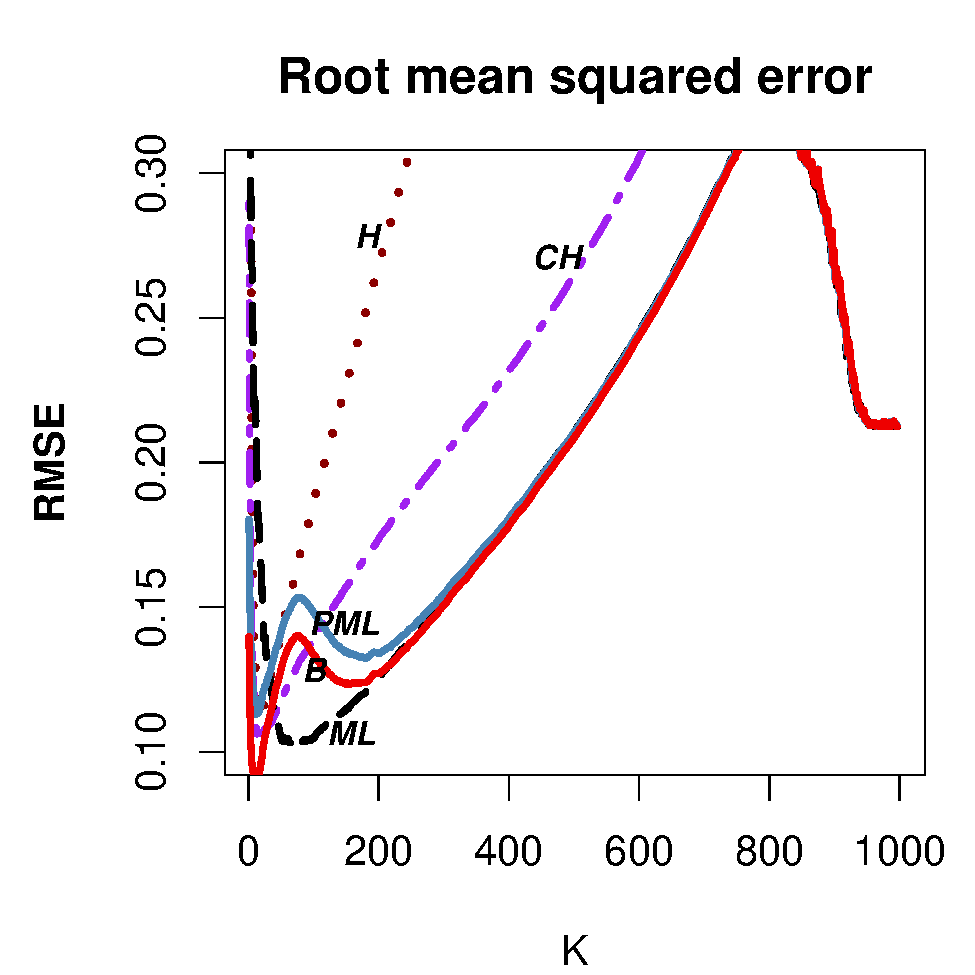
\includegraphics[width=\textwidth]{./plots/paper1/RMSE_OutputGEV0,251000.pdf}
		\end{subfigure}
	\caption{Bias (left) and root mean squared error (right) in case of the \textbf{EV distribution} with $\gamma=0.25$ for sample sizes $n=200$ (top), $n=500$ (middle) and $n=1000$ (bottom) for the Hill estimator (H), the EPD-ML estimator $\hat{\gamma}_{k}^{ML}$ (ML), the penalised ML estimator $\hat{\gamma}^P_{k}(1)$ with $\omega=1$ (PML), the Bayesian estimator $\hat{\gamma}^B_{k}(1)$ with $\omega=1$ (B), and the minimum variance reduced bias estimator $CH_k$ (CH).}
	\label{paper1:fig1}
\end{figure}
	\begin{figure}[h]
		\centering
		\begin{subfigure}[h]{0.40\linewidth}
			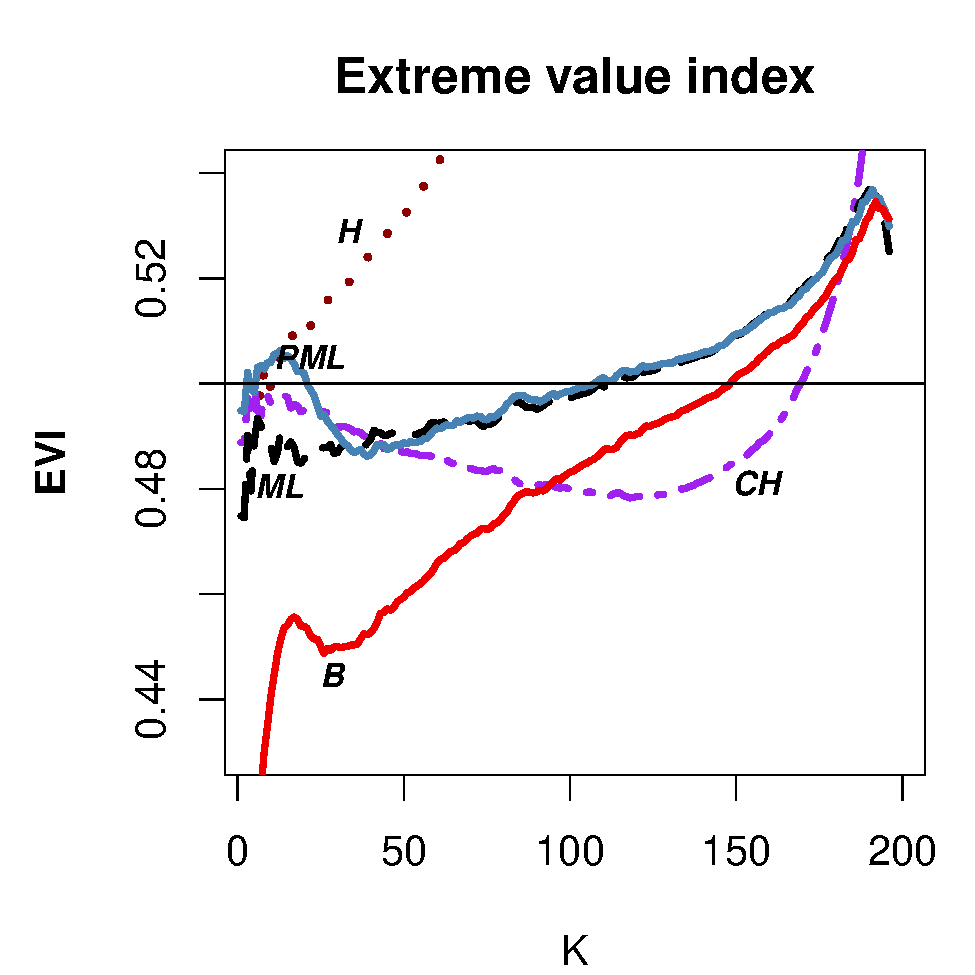
\includegraphics[width=\textwidth]{./plots/paper1/EVI_Outputfrehet0,5200.pdf}
		\end{subfigure}
		\hspace{\fill}
		\begin{subfigure}[h]{0.40\linewidth}
			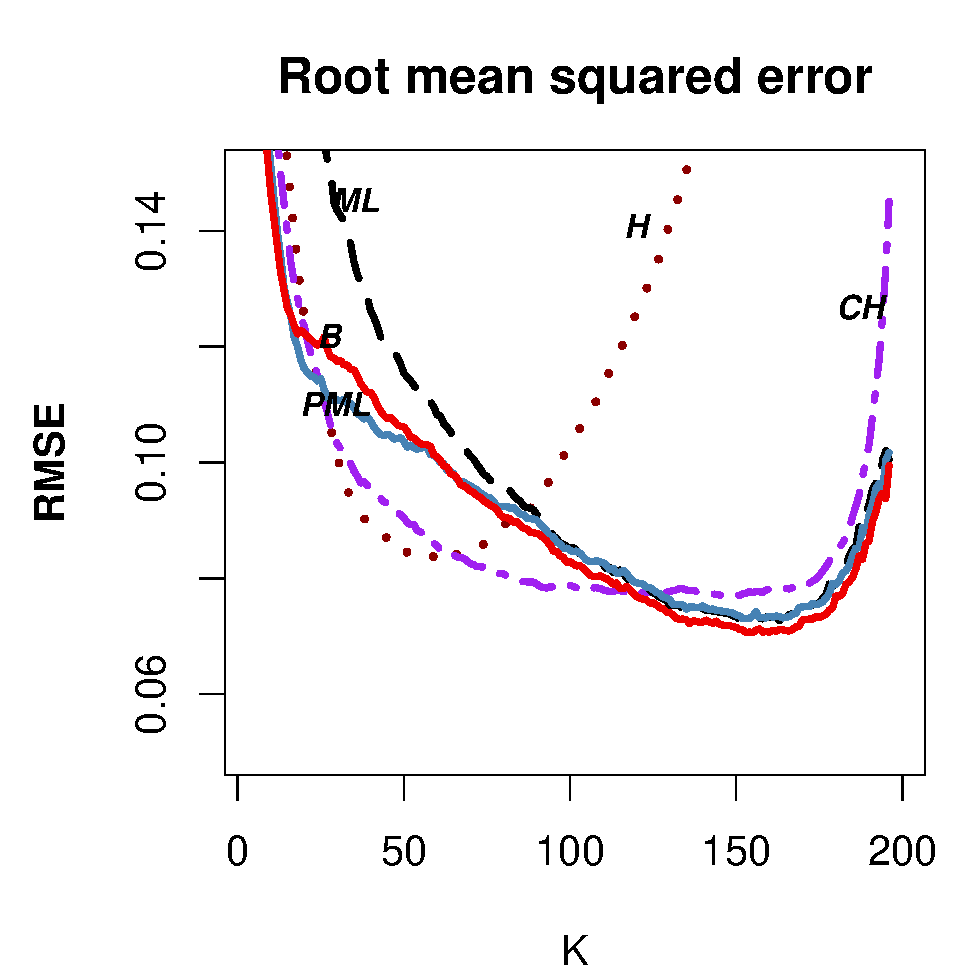
\includegraphics[width=\textwidth]{./plots/paper1/RMSE_Outputfrehet0,5200.pdf}
		\end{subfigure}
		\bigskip
		\centering
		\begin{subfigure}[h]{0.40\linewidth}
			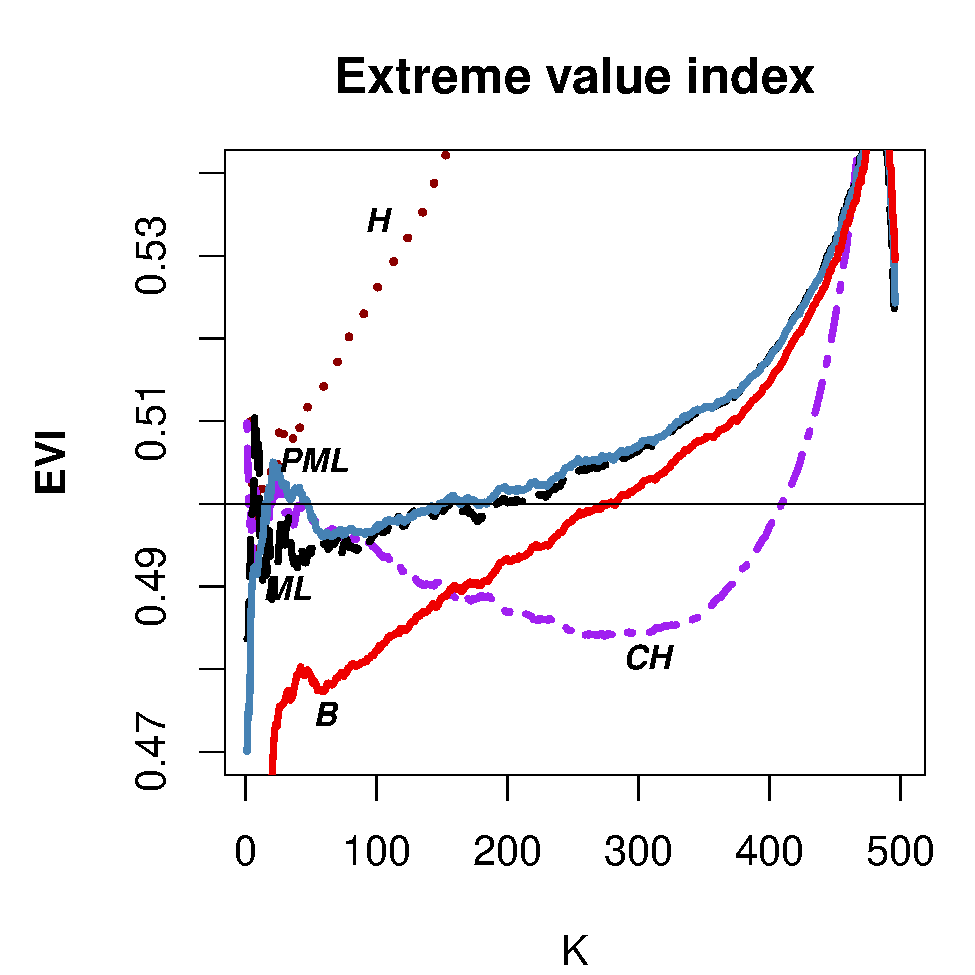
\includegraphics[width=\textwidth]{./plots/paper1/EVI_Outputfrehet0,5500.pdf}
		\end{subfigure}
		\hspace{\fill}
		\begin{subfigure}[h]{0.40\linewidth}
			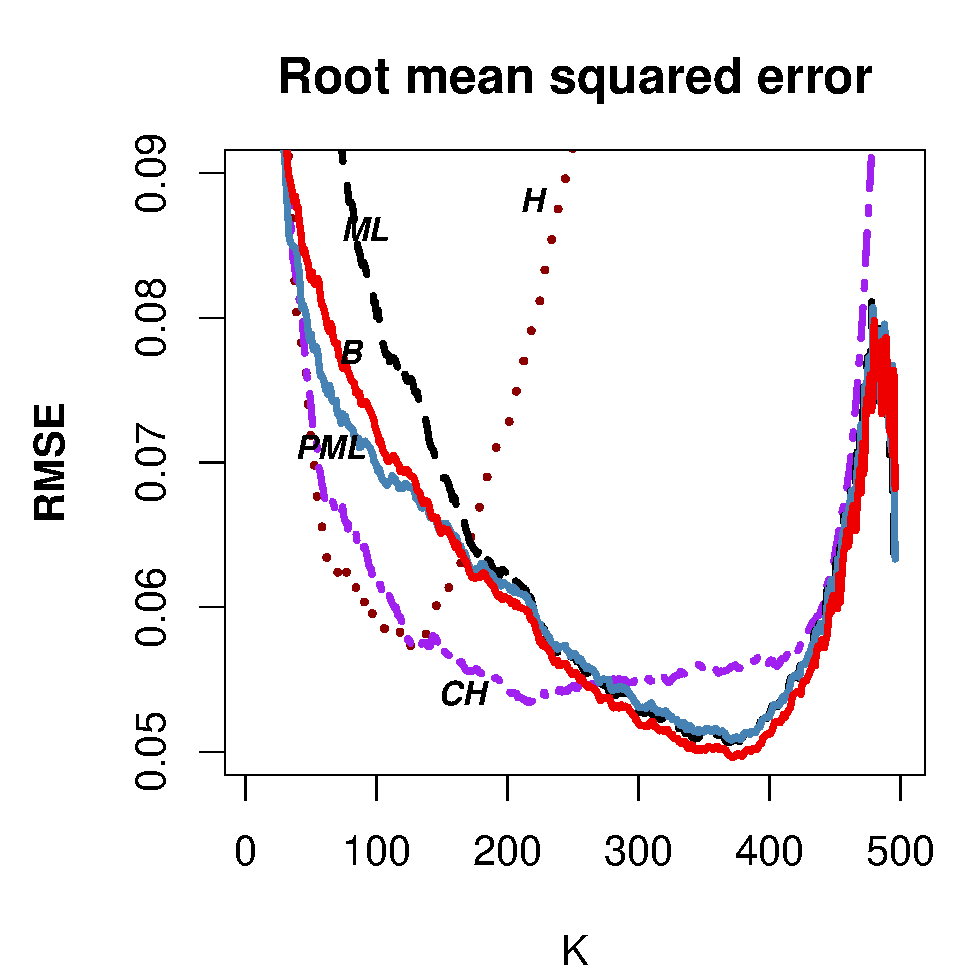
\includegraphics[width=\textwidth]{./plots/paper1/RMSE_Outputfrehet0,5500.pdf}
		\end{subfigure}
		\bigskip
		\centering
		\begin{subfigure}[h]{0.40\linewidth}
			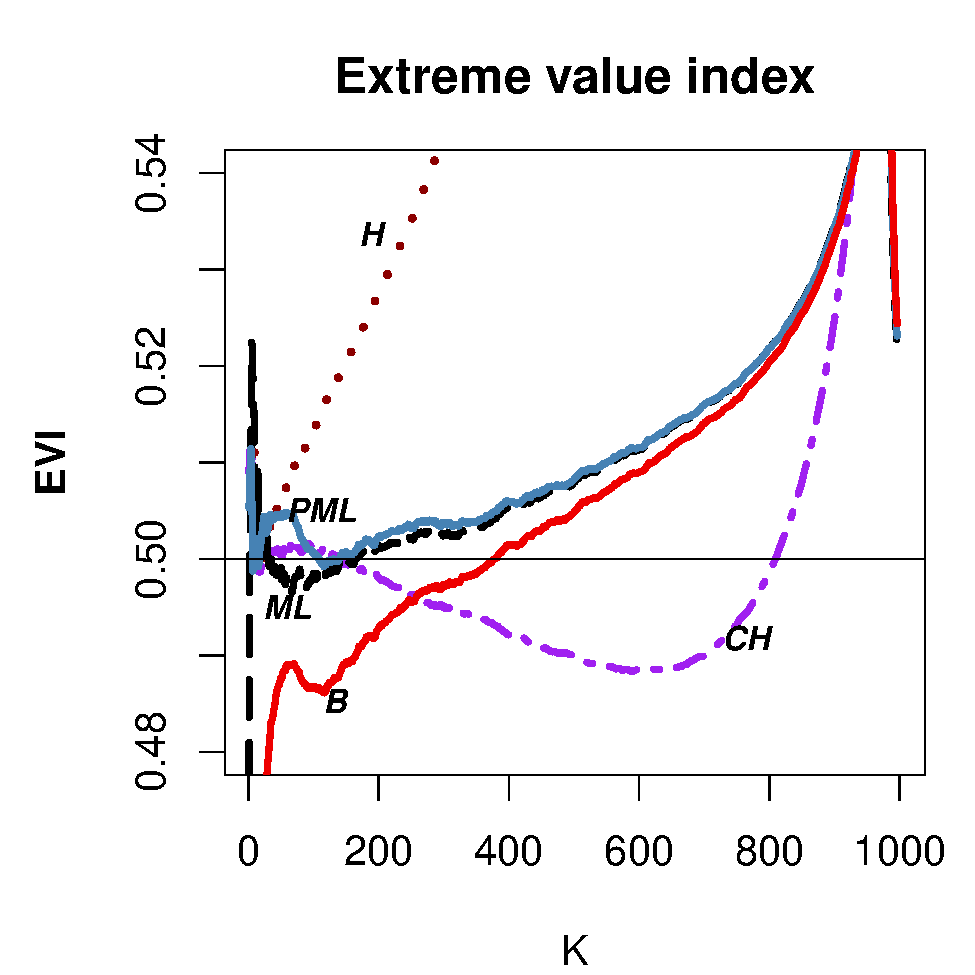
\includegraphics[width=\textwidth]{./plots/paper1/EVI_Outputfrehet0,51000.pdf}
		\end{subfigure}
		\hspace{\fill}
		\begin{subfigure}[h]{0.40\linewidth}
			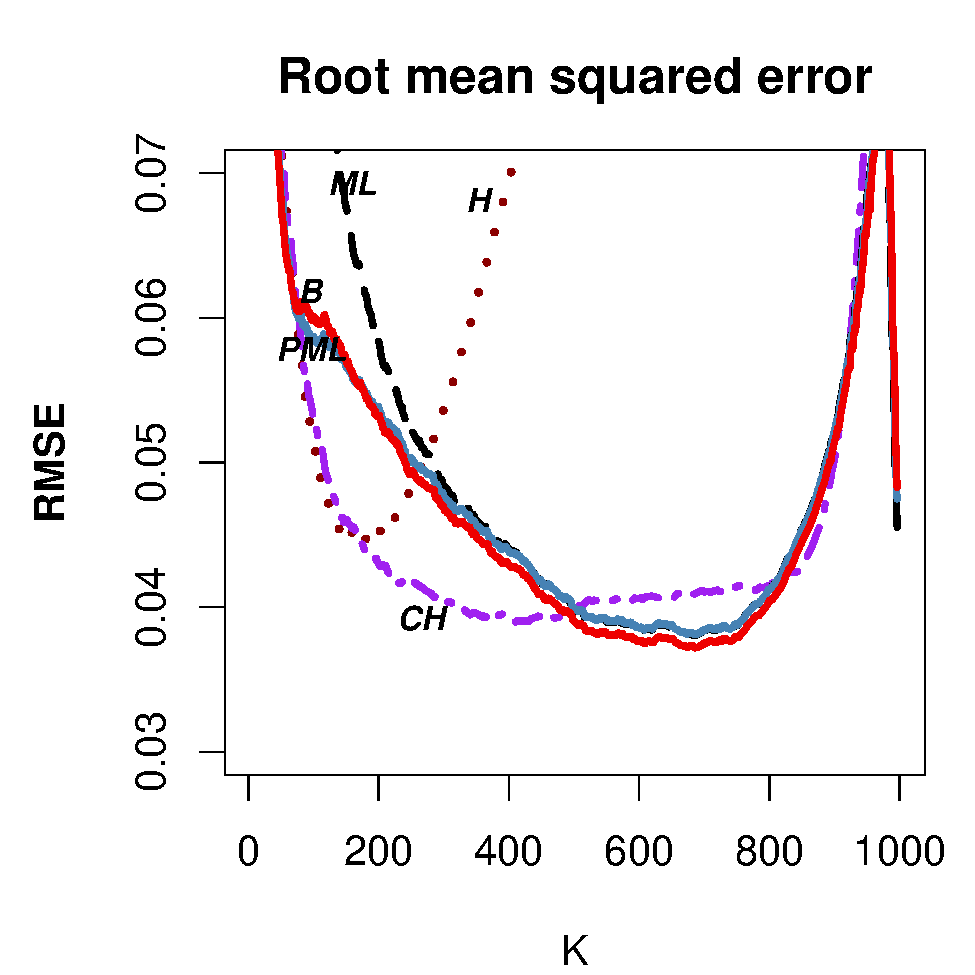
\includegraphics[width=\textwidth]{./plots/paper1/RMSE_Outputfrehet0,51000.pdf}
		\end{subfigure}
		\caption{Bias (left) and root mean squared error (right) in case of the \textbf{Fr\'echet distribution} with $\gamma=0.5$ for sample sizes $n=200$ (top), $n=500$ (middle) and $n=1000$ (bottom) for the Hill estimator (H), the EPD-ML estimator $\hat{\gamma}_{k}^{ML}$ (ML), the penalised ML estimator $\hat{\gamma}^P_{k}(1)$ with $\omega=1$ (PML), the Bayesian estimator $\hat{\gamma}^B_{k}(1)$ with $\omega=1$ (B), and the minimum variance reduced bias estimator $CH_k$ (CH).}
		\label{paper1:fig2}
	\end{figure}
	\begin{figure}[h]
		\centering
		\begin{subfigure}[h]{0.40\linewidth}
			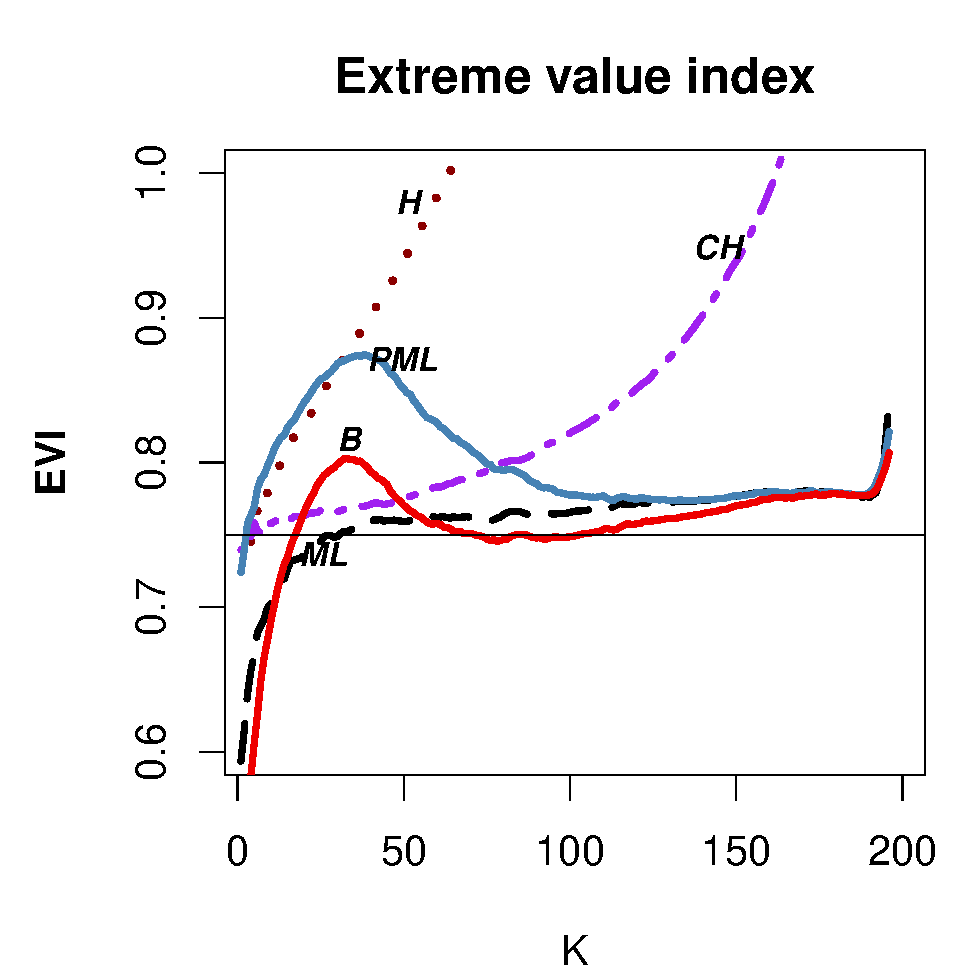
\includegraphics[width=\textwidth]{./plots/paper1/EVI_Outputburr0,75200.pdf}
		\end{subfigure}
		\hspace{\fill}
		\begin{subfigure}[h]{0.40\linewidth}
			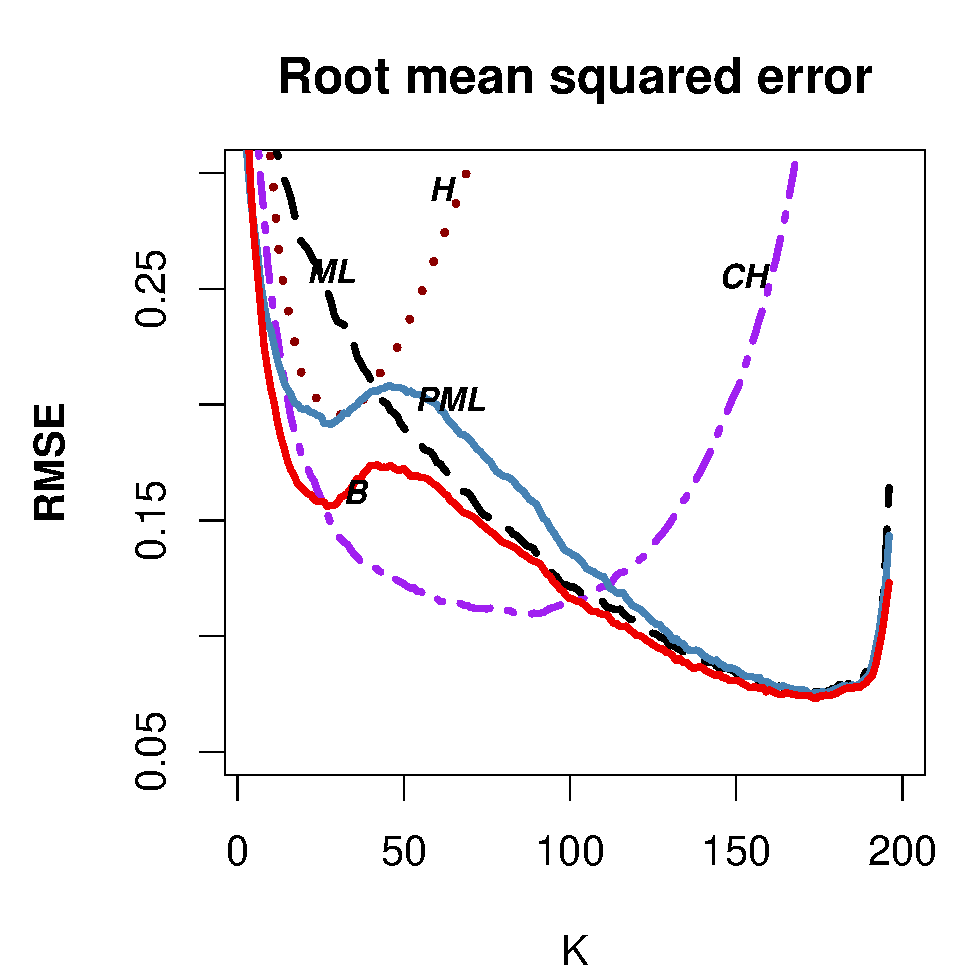
\includegraphics[width=\textwidth]{./plots/paper1/RMSE_Outputburr0,75200.pdf}
		\end{subfigure}
		\bigskip
		\centering
		\begin{subfigure}[h]{0.40\linewidth}
			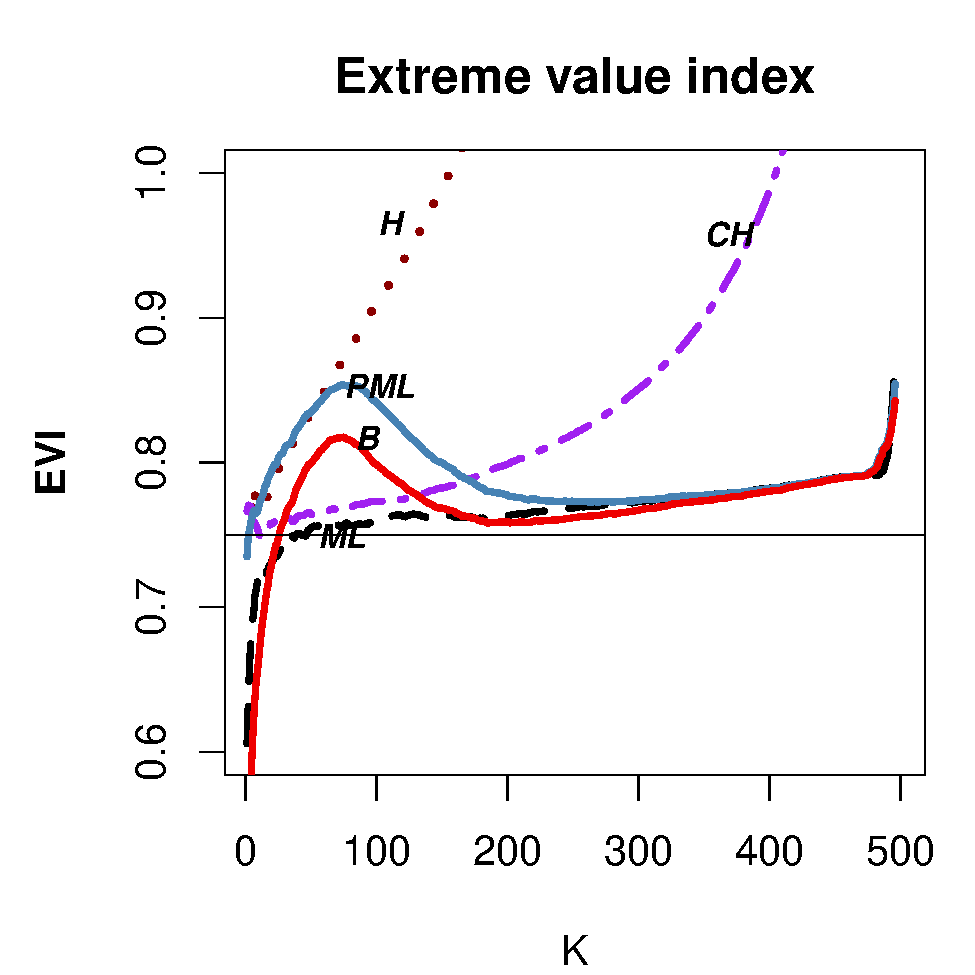
\includegraphics[width=\textwidth]{./plots/paper1/EVI_Outputburr0,75500.pdf}
		\end{subfigure}
		\hspace{\fill}
		\begin{subfigure}[h]{0.40\linewidth}
			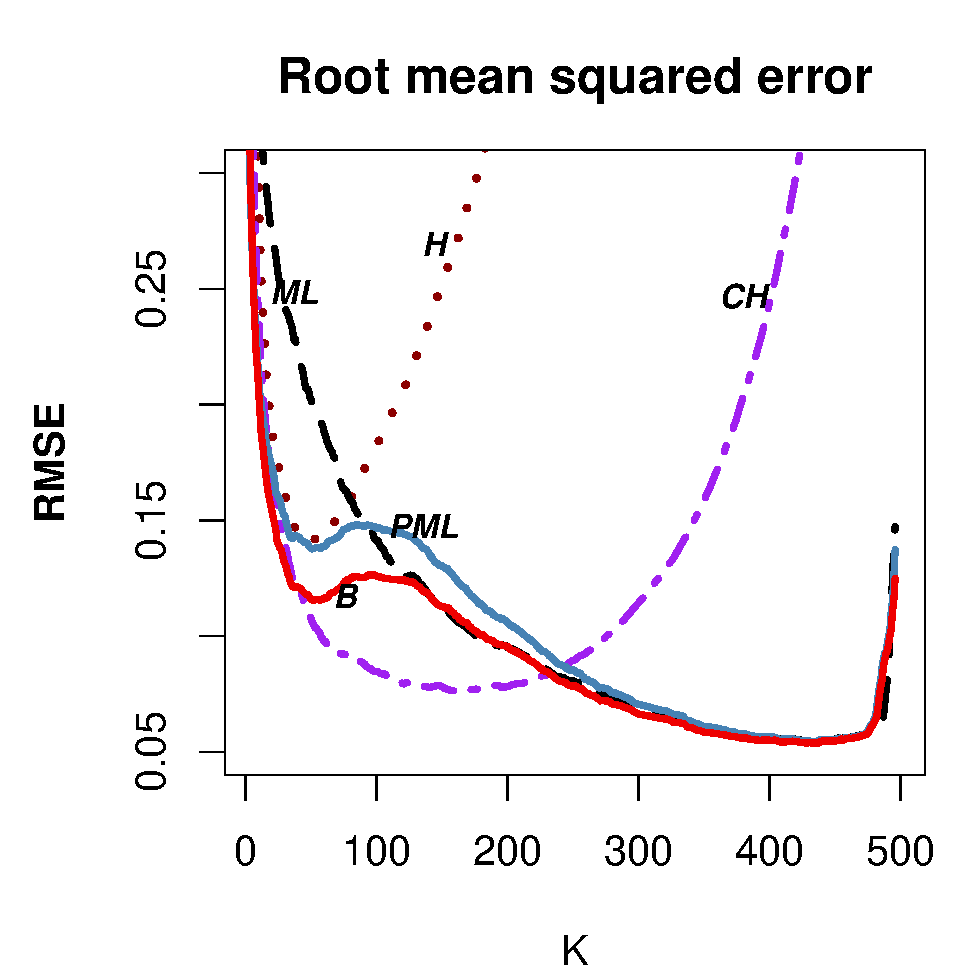
\includegraphics[width=\textwidth]{./plots/paper1/RMSE_Outputburr0,75500.pdf}
		\end{subfigure}
		\bigskip
		\centering
		\begin{subfigure}[h]{0.40\linewidth}
			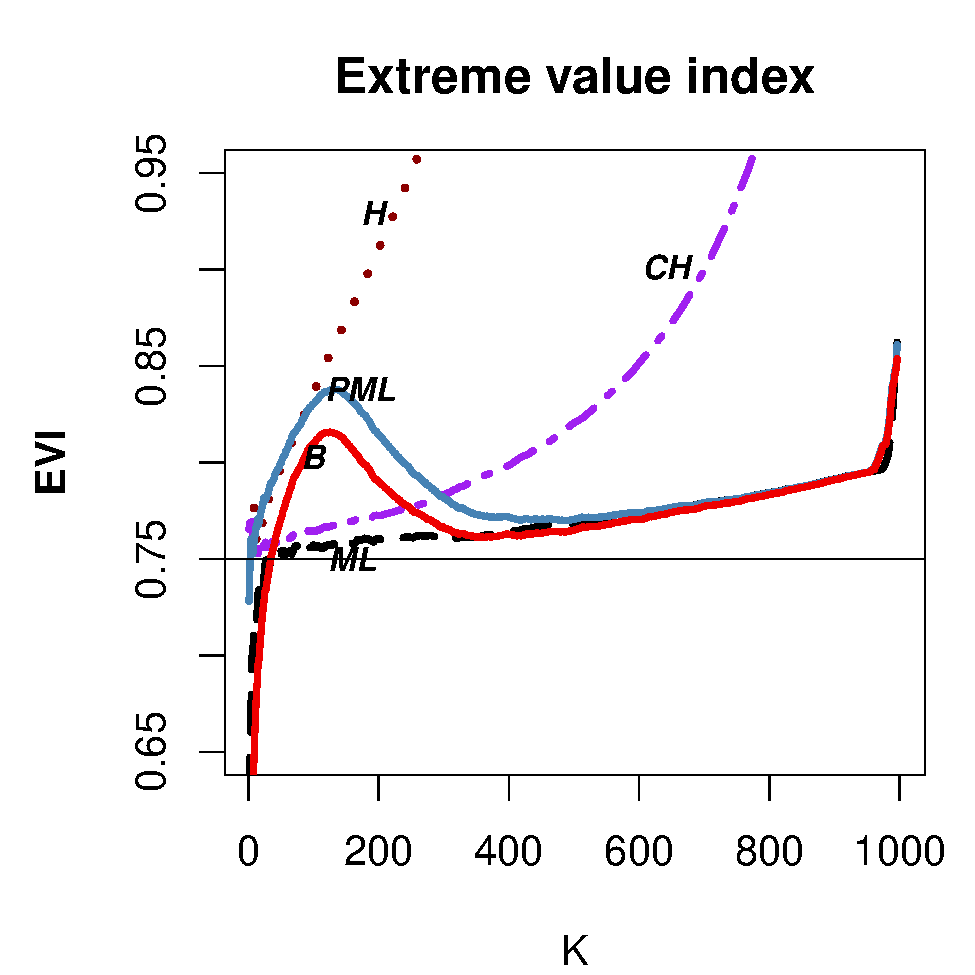
\includegraphics[width=\textwidth]{./plots/paper1/EVI_Outputburr0,751000.pdf}
		\end{subfigure}
		\hspace{\fill}
		\begin{subfigure}[h]{0.40\linewidth}
			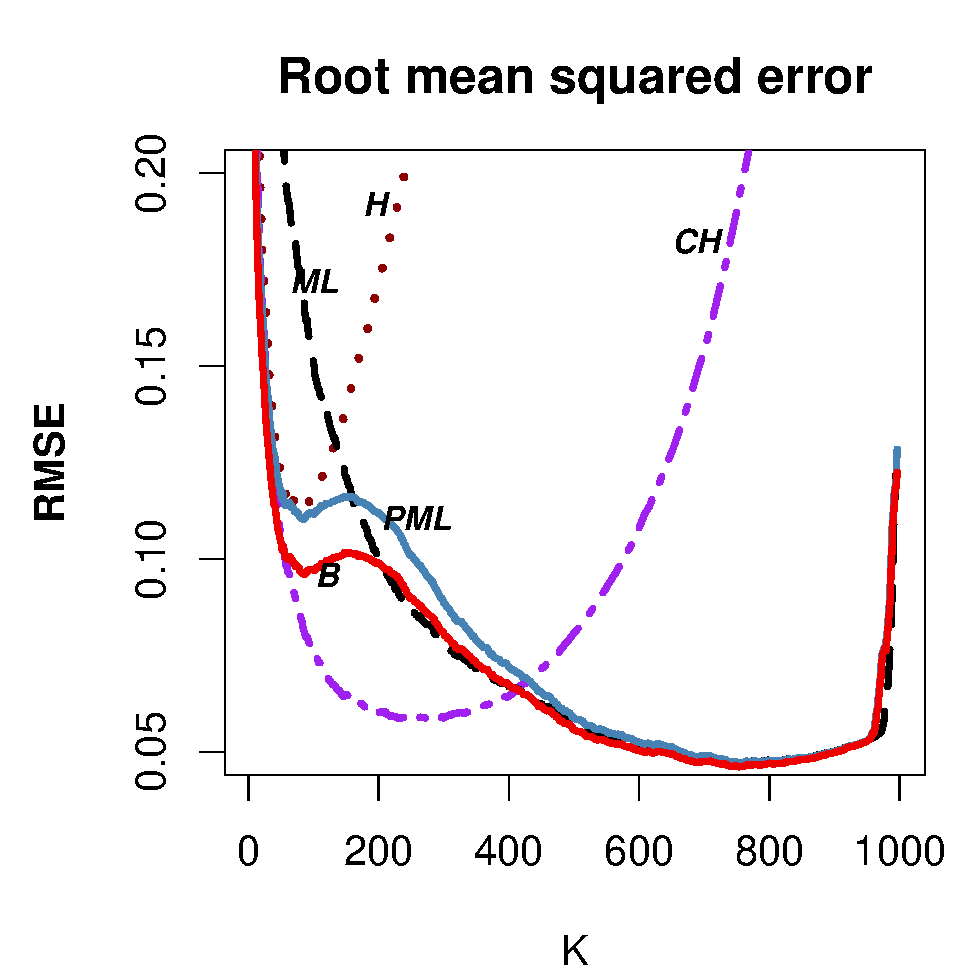
\includegraphics[width=\textwidth]{./plots/paper1/RMSE_Outputburr0,751000.pdf}
		\end{subfigure}
		\caption{Bias (left) and root mean squared error (right) in case of the \textbf{Burr distribution} with $\gamma=0.75$ for sample sizes $n=200$ (top), $n=500$ (middle) and $n=1000$ (bottom) for the Hill estimator (H), the EPD-ML estimator $\hat{\gamma}_{k}^{ML}$ (ML), the penalised ML estimator $\hat{\gamma}^P_{k}(1)$ with $\omega=1$ (PML), the Bayesian estimator $\hat{\gamma}^B_{k}(1)$ with $\omega=1$ (B), and the minimum variance reduced bias estimator $CH_k$ (CH).}
		\label{paper1:fig3}
	\end{figure}
	\begin{figure}[h]
		\centering
		\begin{subfigure}[h]{0.40\linewidth}
			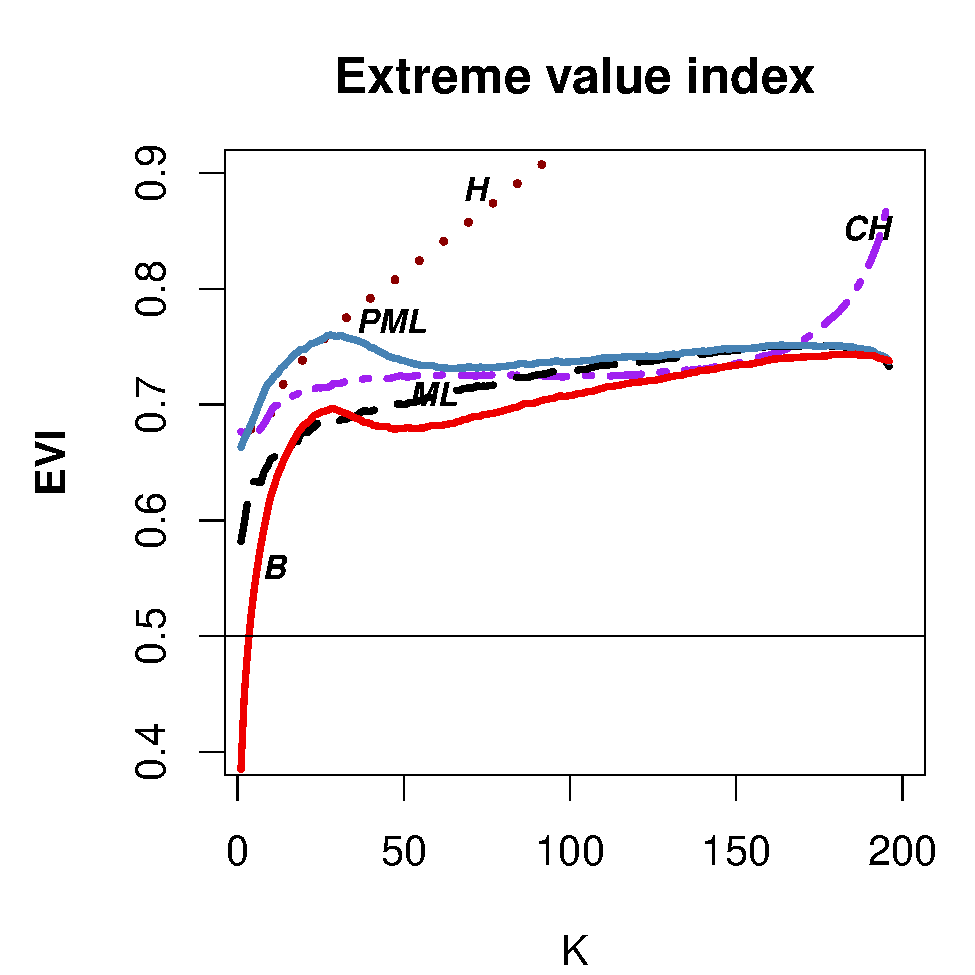
\includegraphics[width=\textwidth]{./plots/paper1/EVI_Outputloggamma0,5200.pdf}
		\end{subfigure}
	\hspace{\fill}
		\begin{subfigure}[h]{0.40\linewidth}
			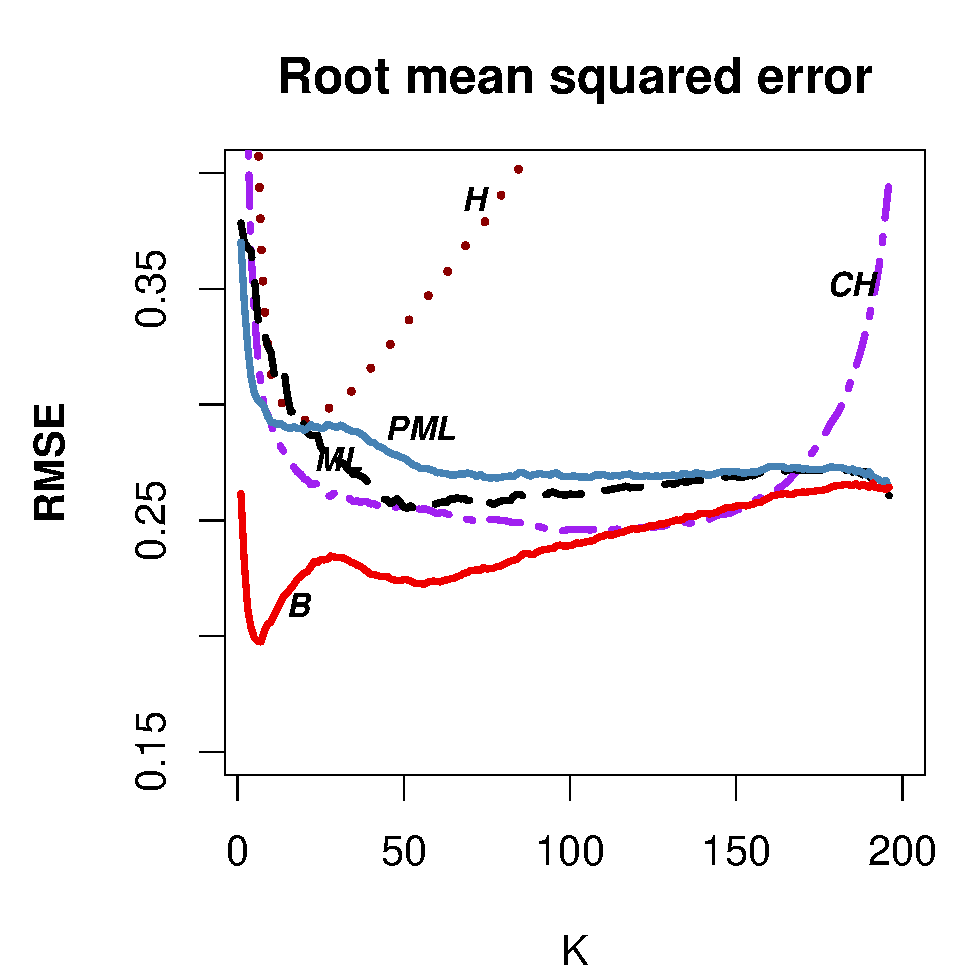
\includegraphics[width=\textwidth]{./plots/paper1/RMSE_Outputloggamma0,5200.pdf}
		\end{subfigure}
		\bigskip
		\centering
		\begin{subfigure}[h]{0.40\linewidth}
			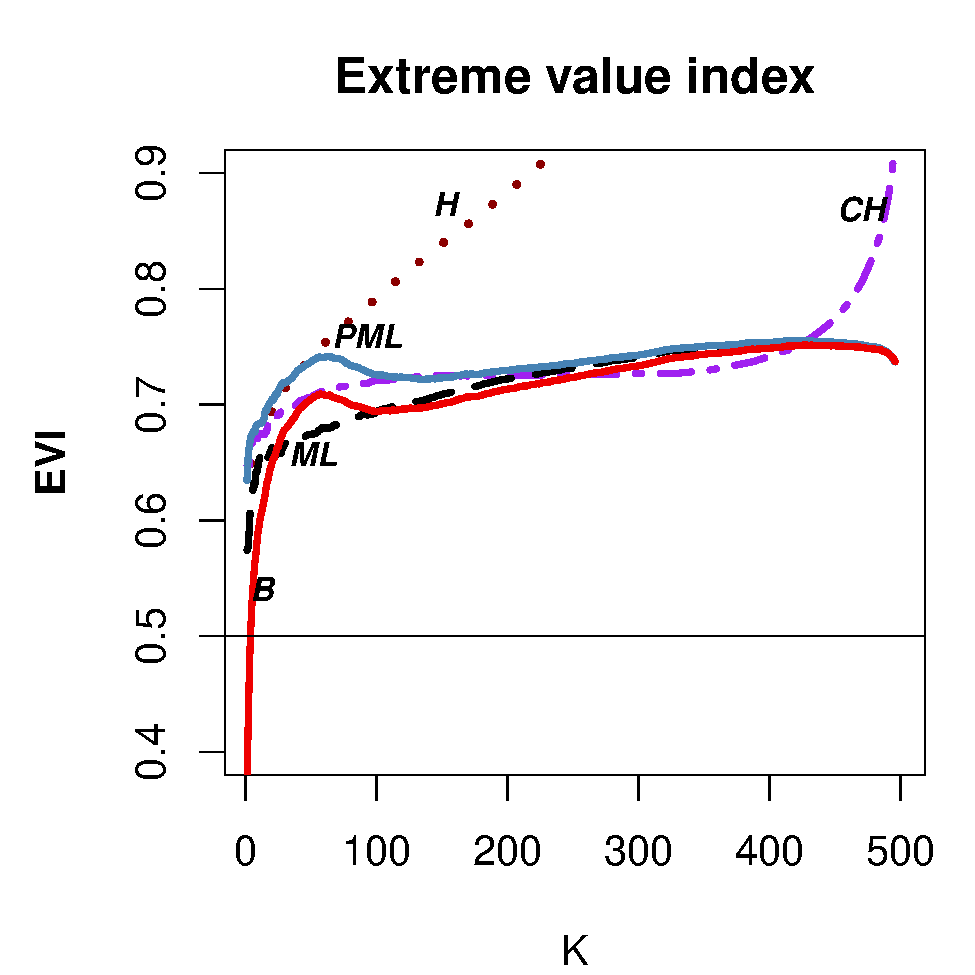
\includegraphics[width=\textwidth]{./plots/paper1/EVI_Outputloggamma0,5500.pdf}
		\end{subfigure}
		\hspace{\fill}
		\begin{subfigure}[h]{0.40\linewidth}
			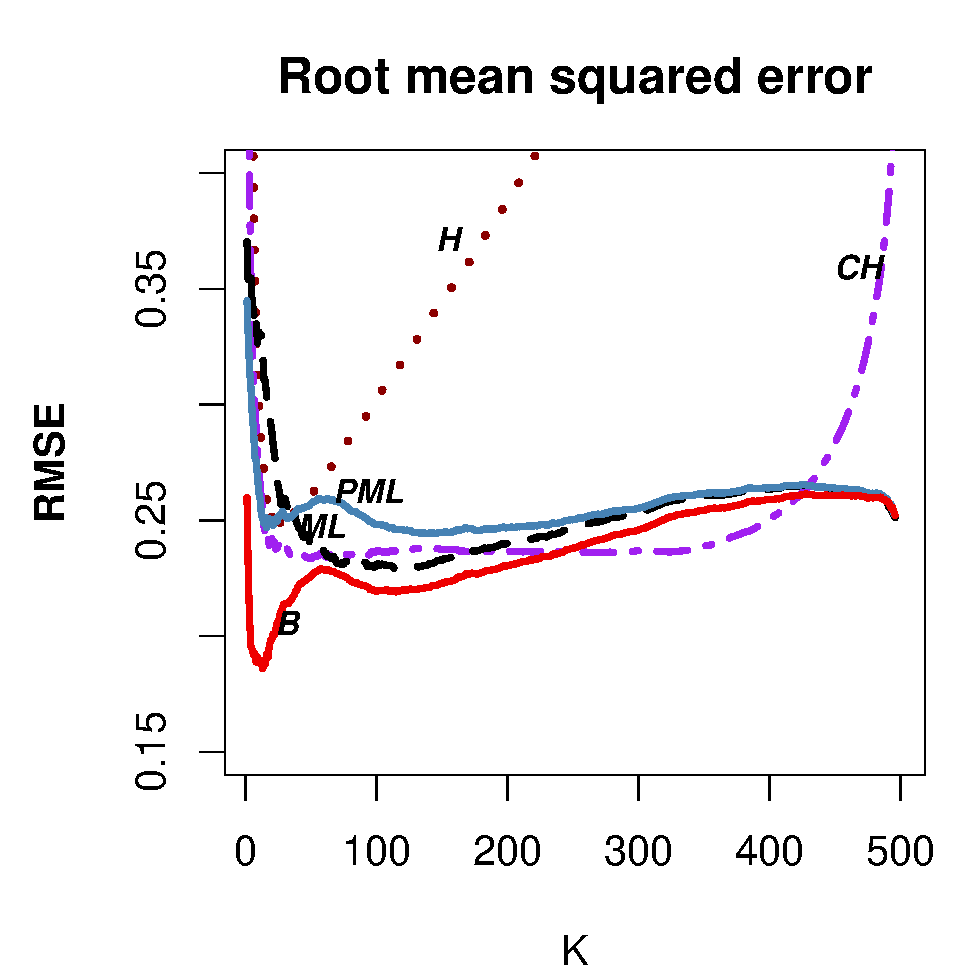
\includegraphics[width=\textwidth]{./plots/paper1/RMSE_Outputloggamma0,5500.pdf}
		\end{subfigure}
		\bigskip
		\centering
		\begin{subfigure}[h]{0.40\linewidth}
			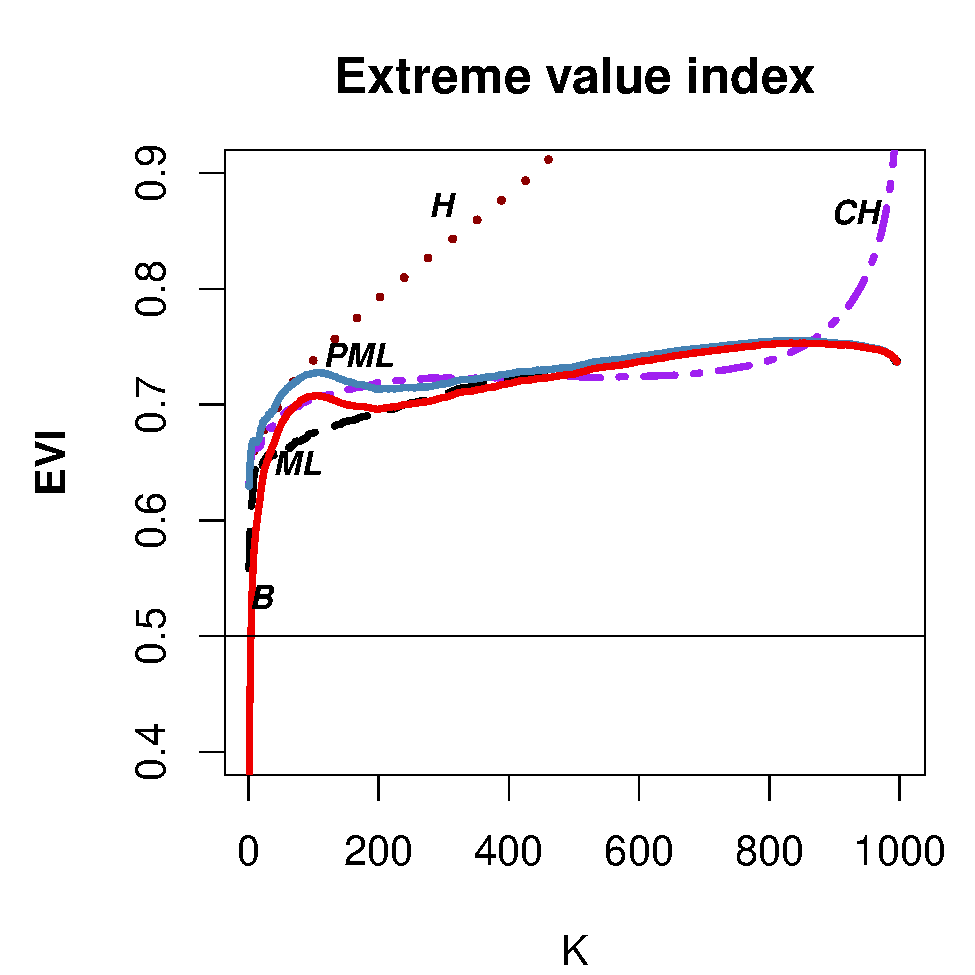
\includegraphics[width=\textwidth]{./plots/paper1/EVI_Outputloggamma0,51000.pdf}
		\end{subfigure}
		\hspace{\fill}
		\begin{subfigure}[h]{0.40\linewidth}
			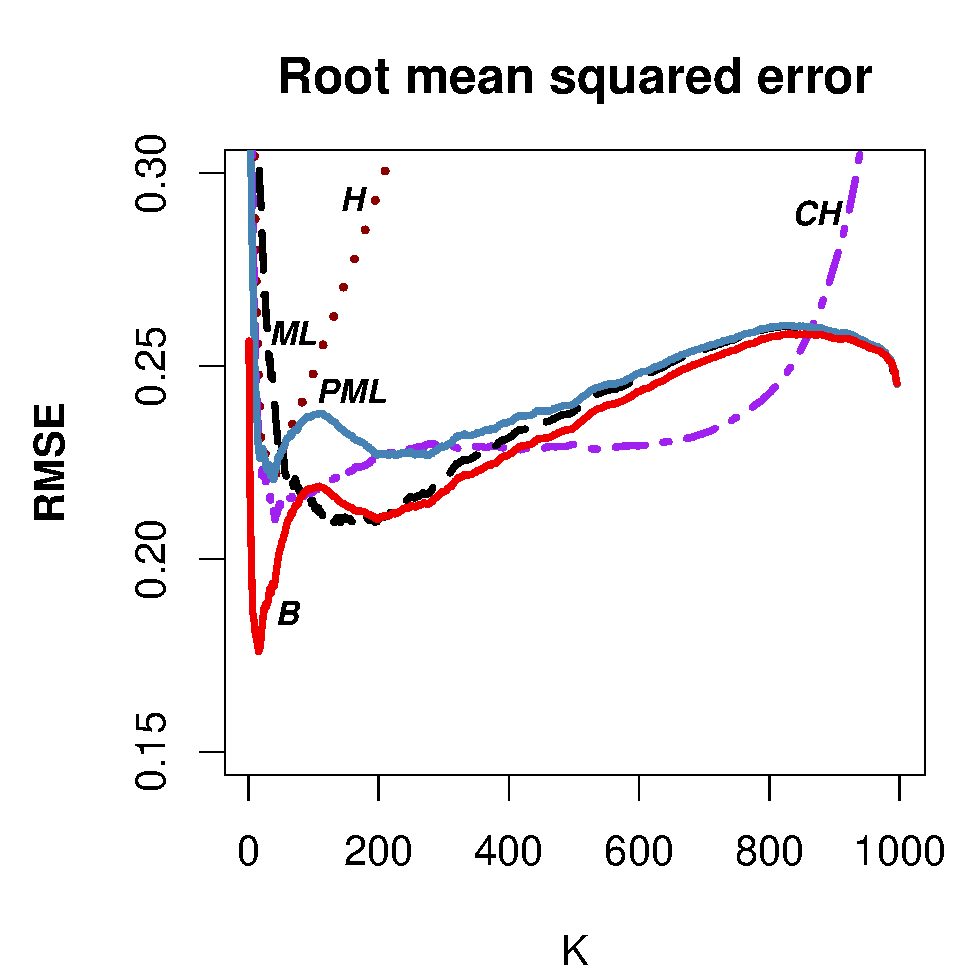
\includegraphics[width=\textwidth]{./plots/paper1/RMSE_Outputloggamma0,51000.pdf}
		\end{subfigure}
		\caption{Bias (left) and root mean squared error (right) in case of the \textbf{loggamma distribution} with $\gamma=0.5$ for sample sizes $n=200$ (top), $n=500$ (middle) and $n=1000$ (bottom) for the Hill estimator (H), the EPD-ML estimator $\hat{\gamma}_{k}^{ML}$ (ML), the penalised ML estimator $\hat{\gamma}^P_{k}(1)$ with $\omega=1$ (PML), the Bayesian estimator $\hat{\gamma}^B_{k}(1)$ with $\omega=1$ (B), and the minimum variance reduced bias estimator $CH_k$ (CH).}
		\label{paper1:fig4}
	\end{figure}
	\begin{figure}[h]
		\centering
		\begin{subfigure}[h]{0.40\linewidth}
			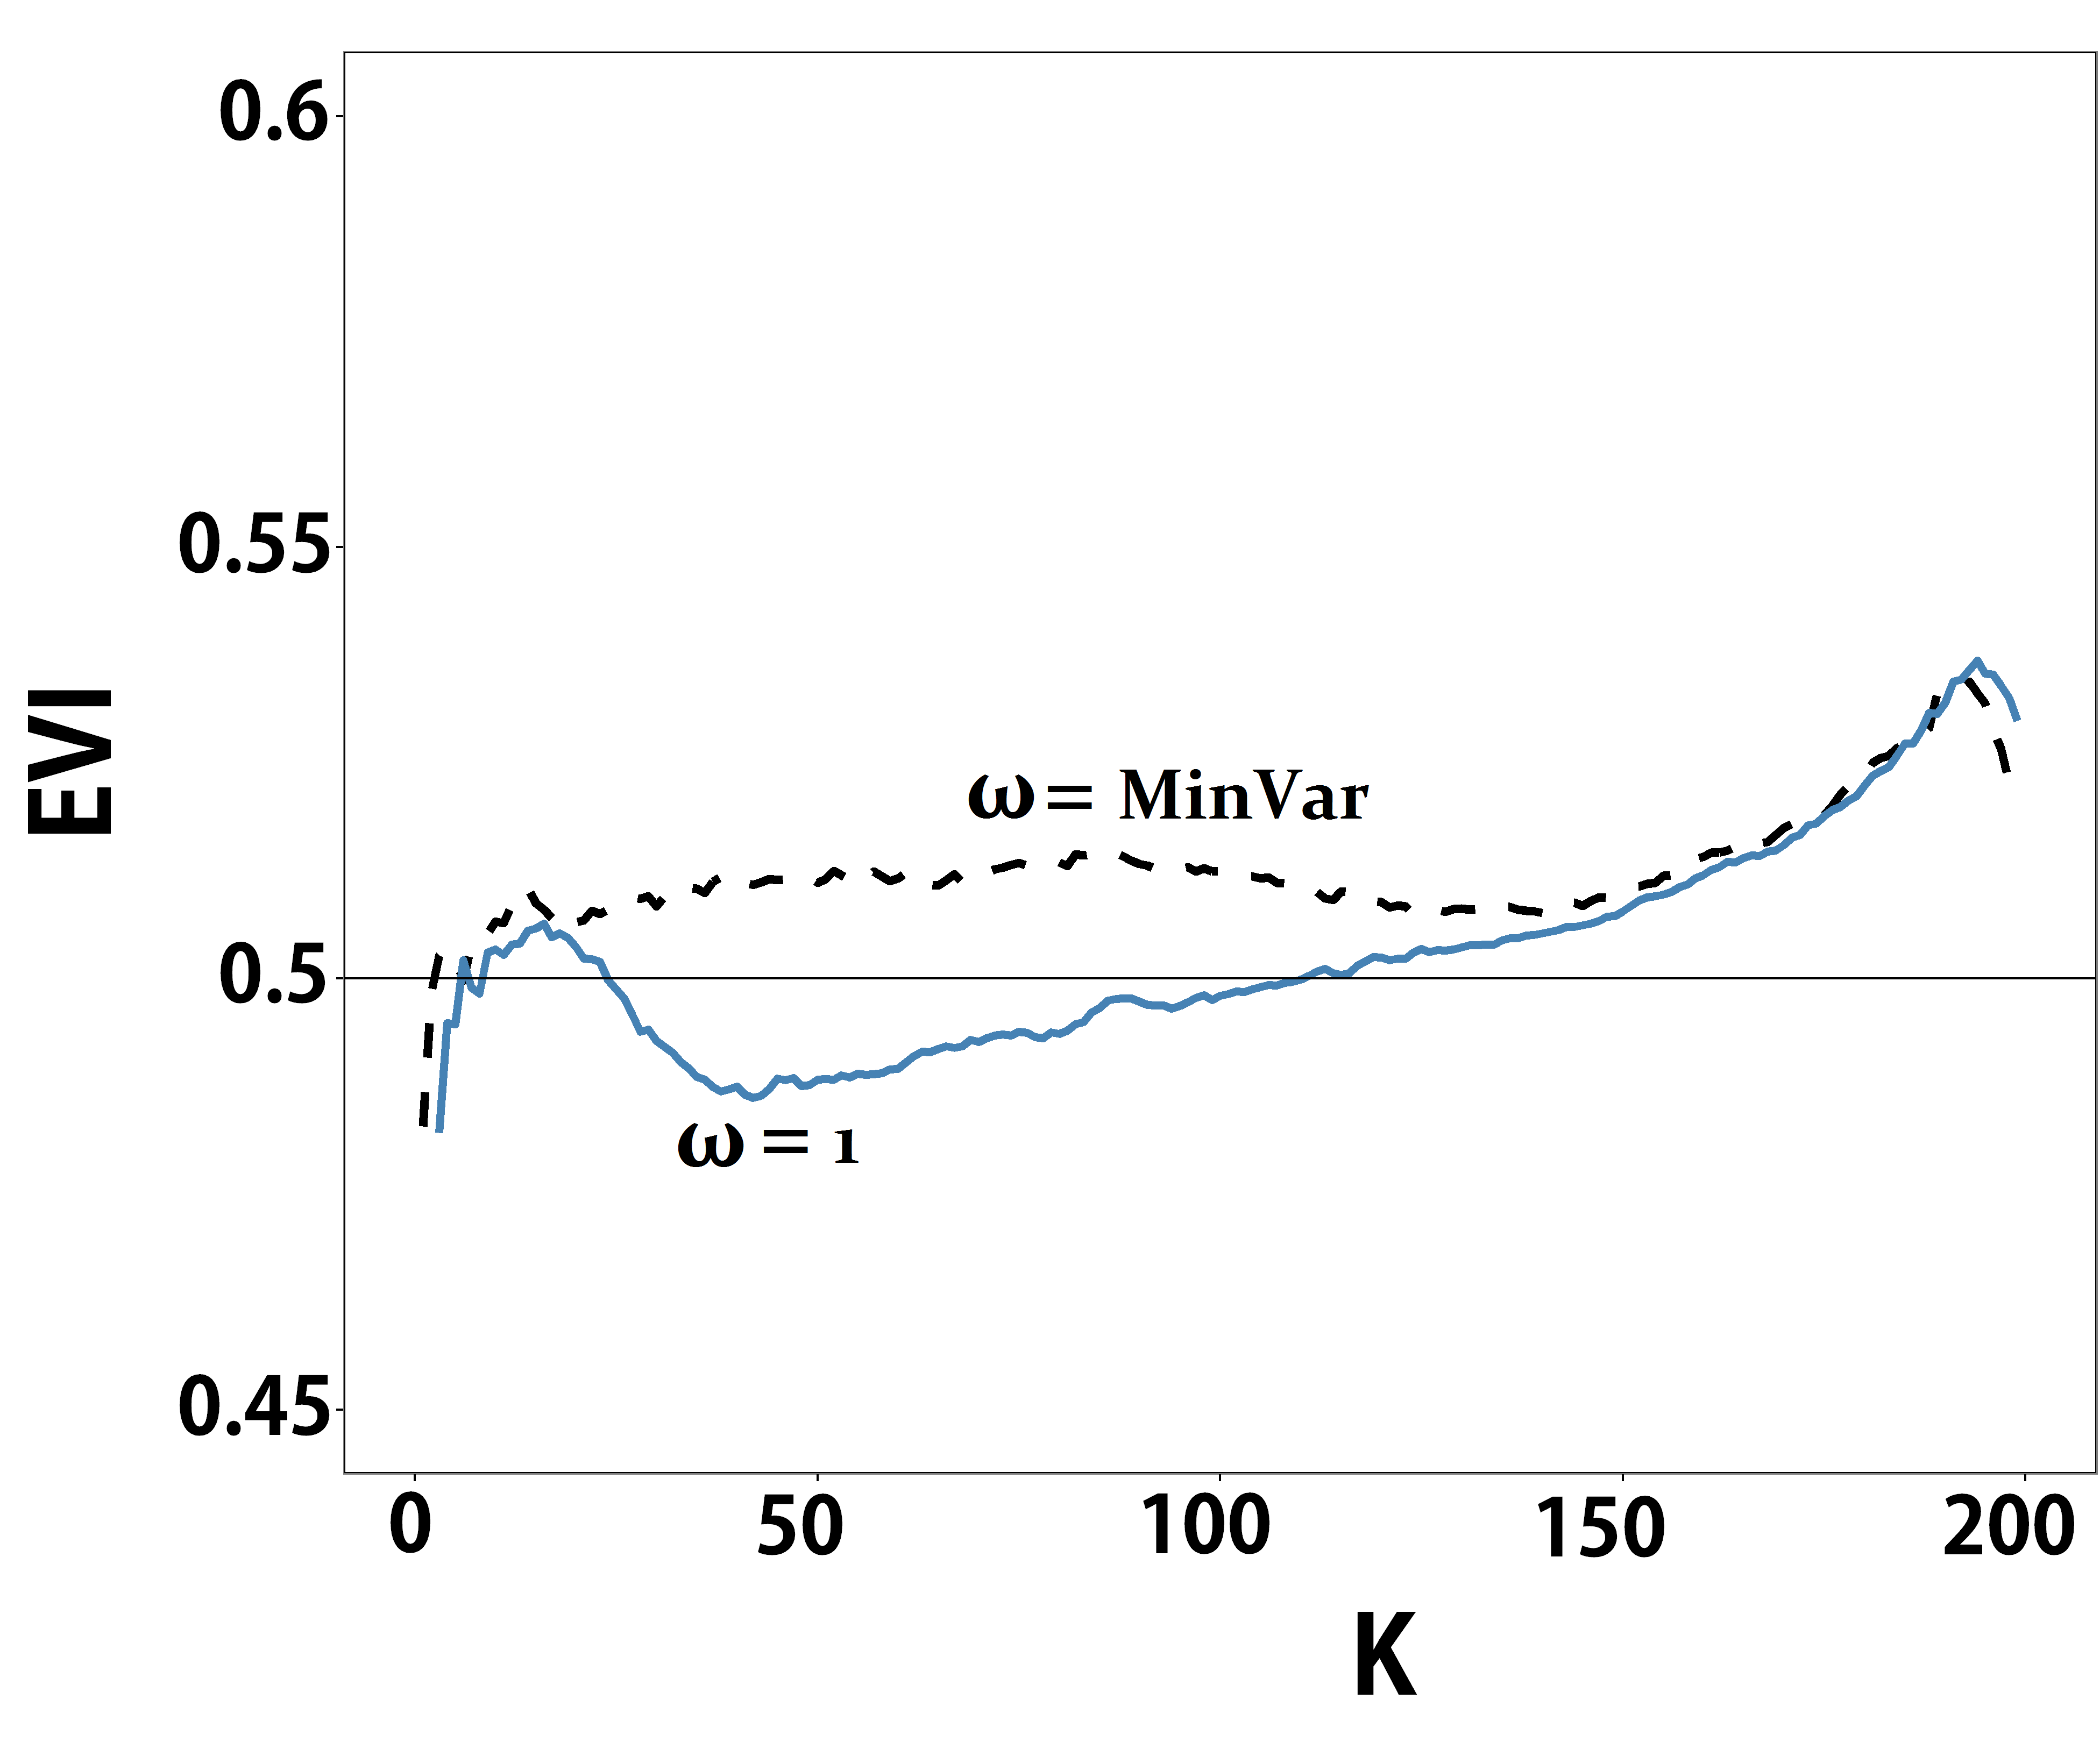
\includegraphics[width=65mm]{./plots/paper1/eviFrechetKappa.png}
		\end{subfigure}
		\hspace{\fill}
		\begin{subfigure}[h]{0.40\linewidth}
			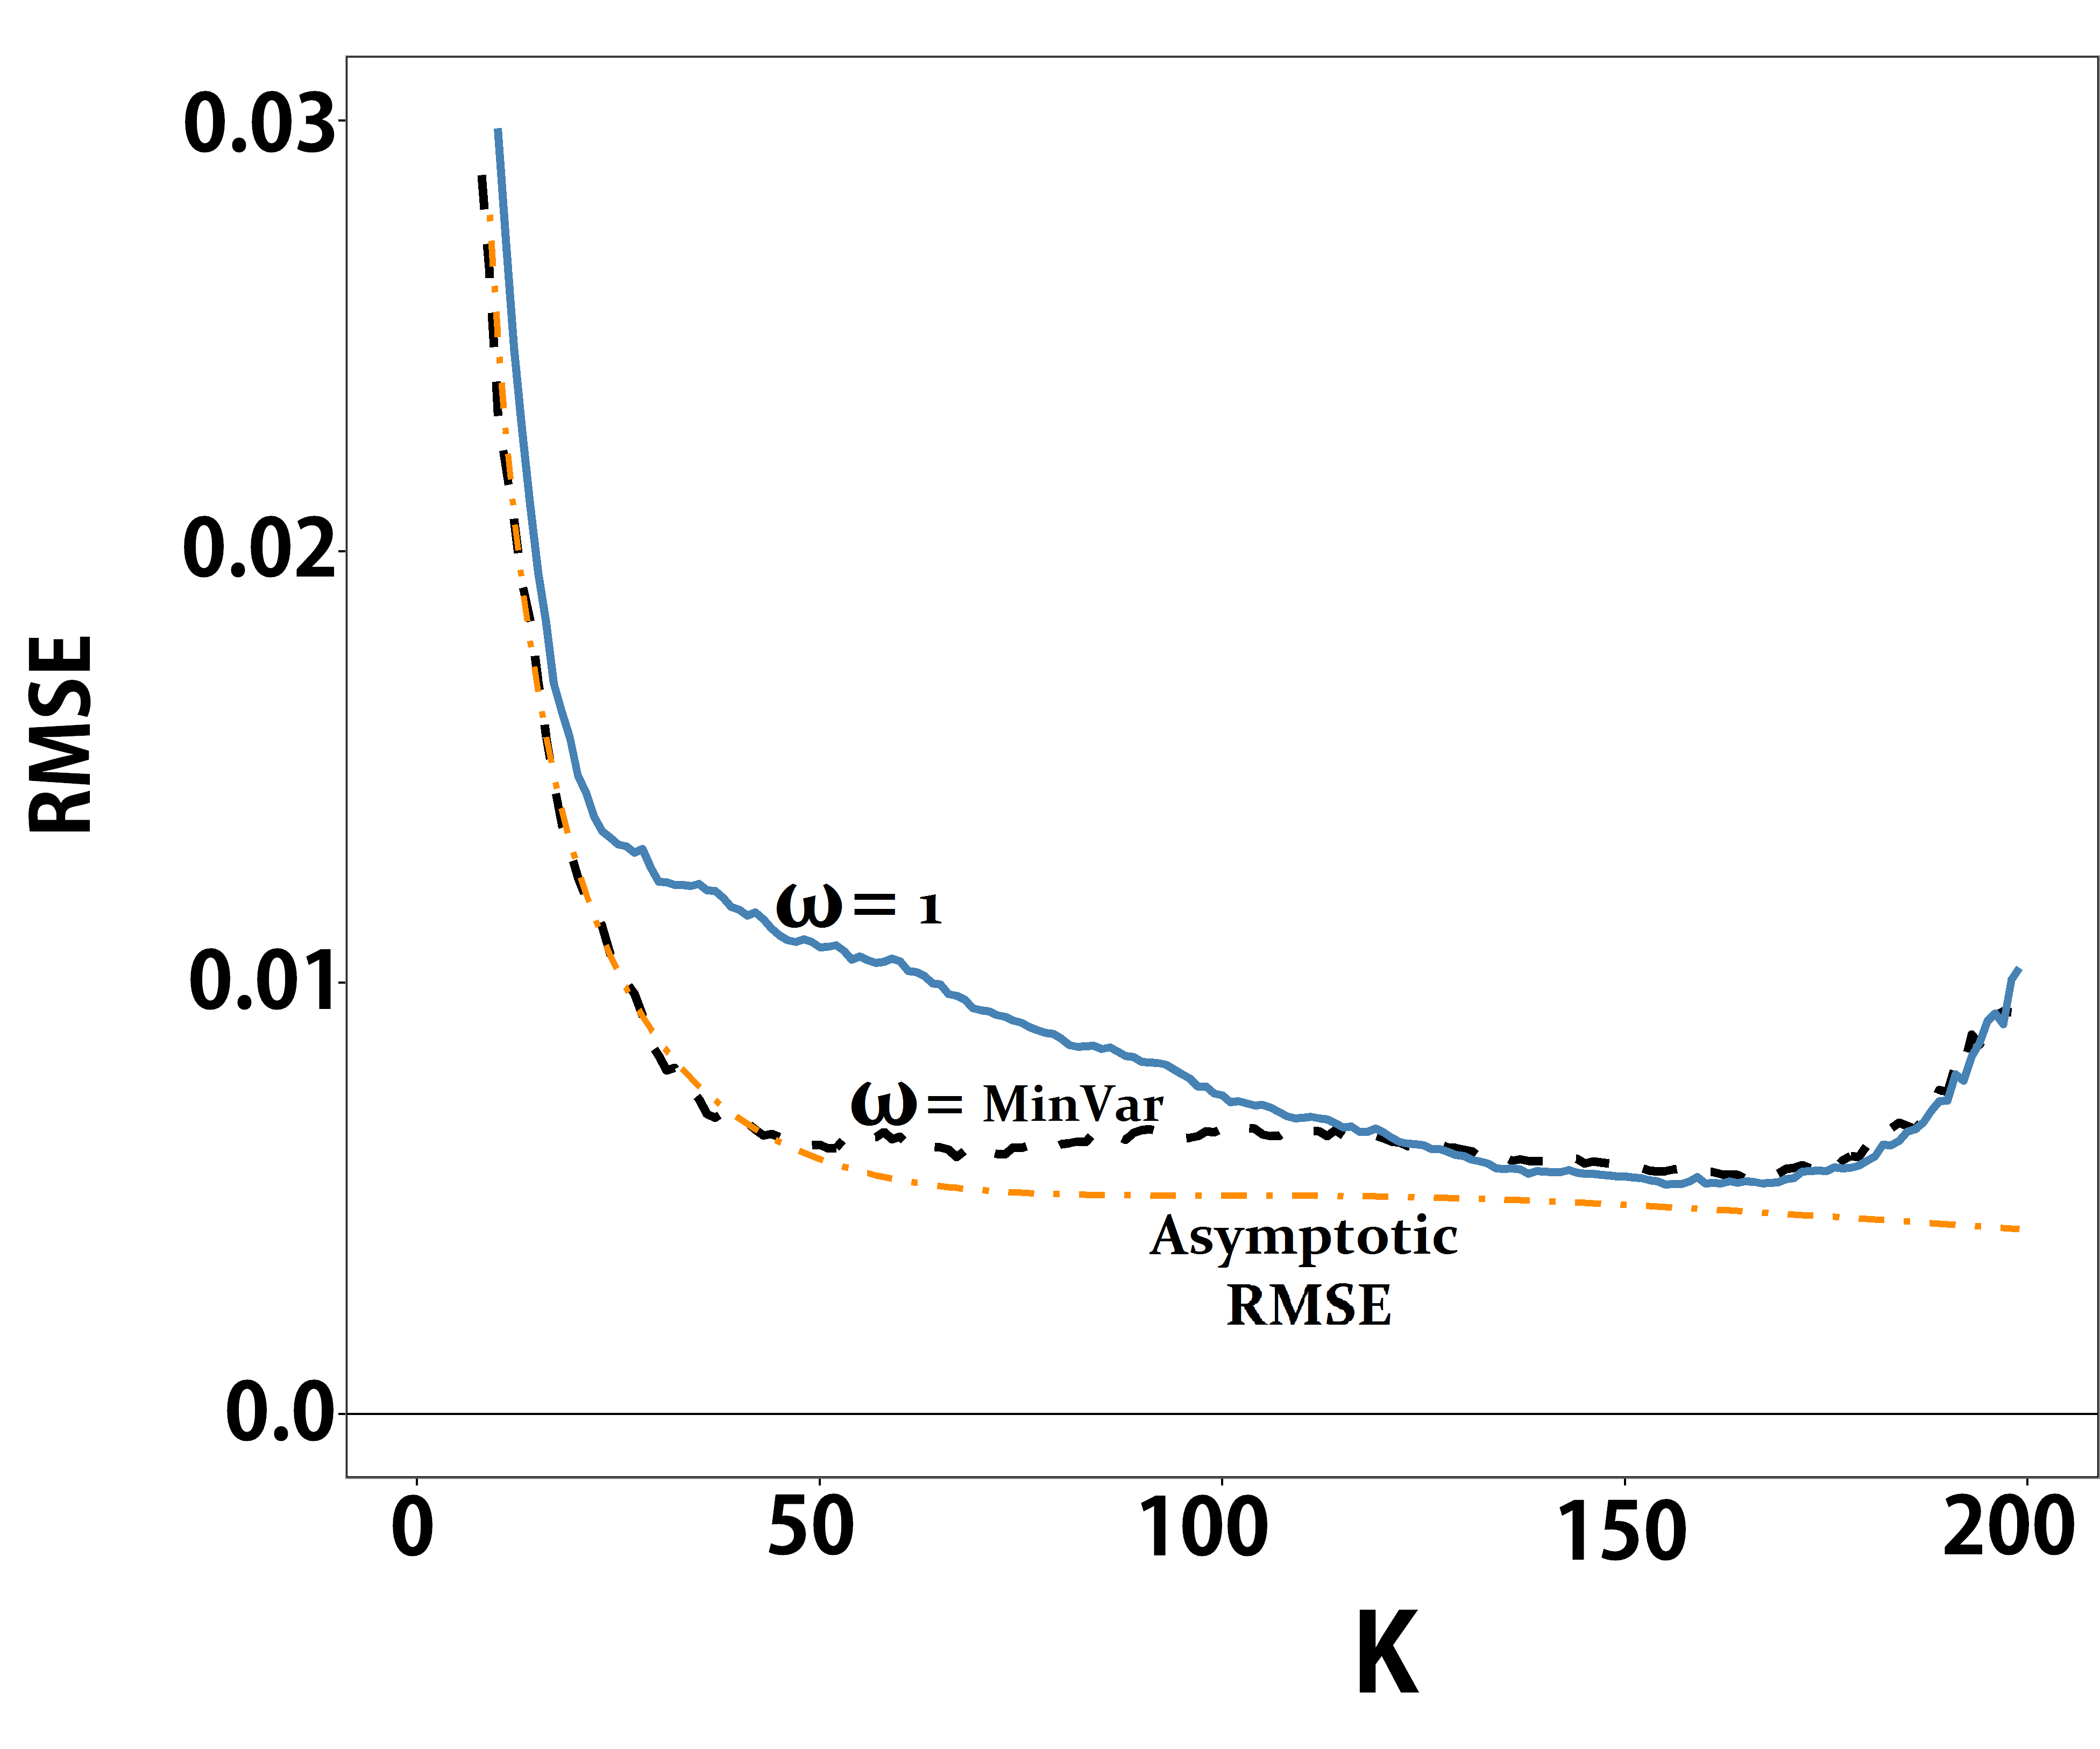
\includegraphics[width=65mm]{./plots/paper1/mseFrechetKappa.png}
		\end{subfigure}
		\bigskip
		\begin{subfigure}[h]{0.40\linewidth}
			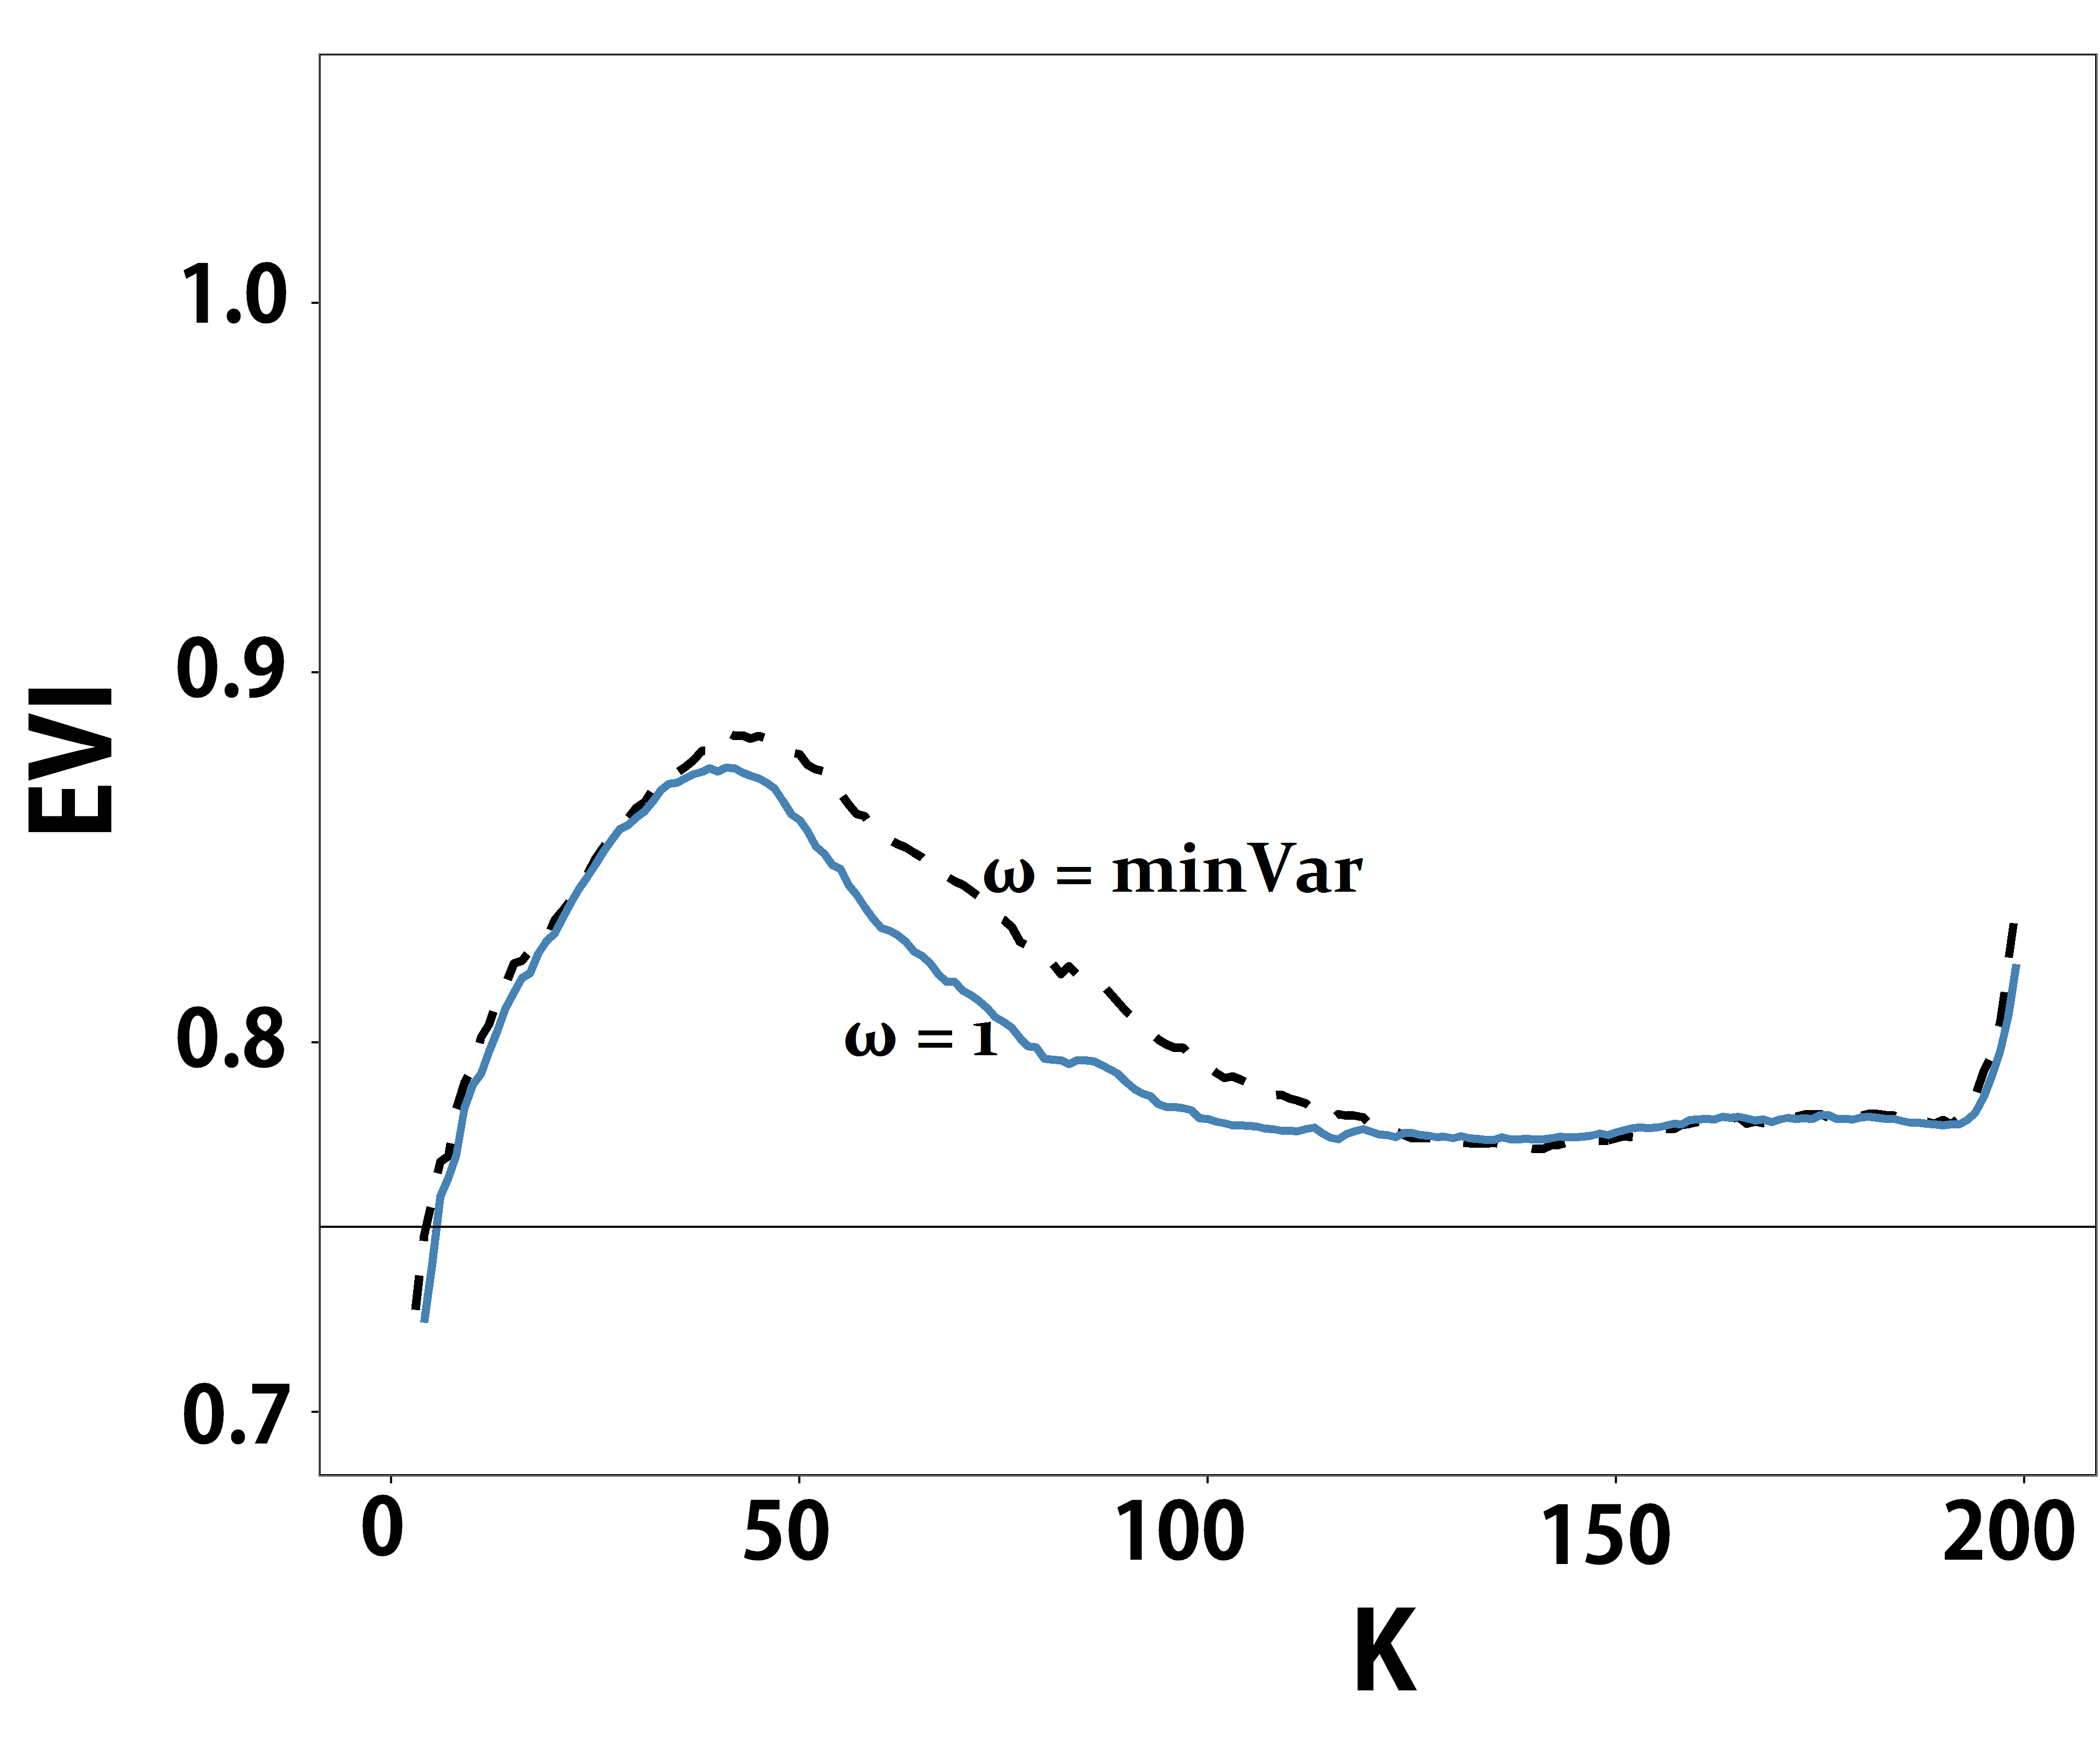
\includegraphics[width=65mm]{./plots/paper1/eviBurrKappa.png}
		\end{subfigure}
		\hspace{\fill}
		\begin{subfigure}[h]{0.40\linewidth}
			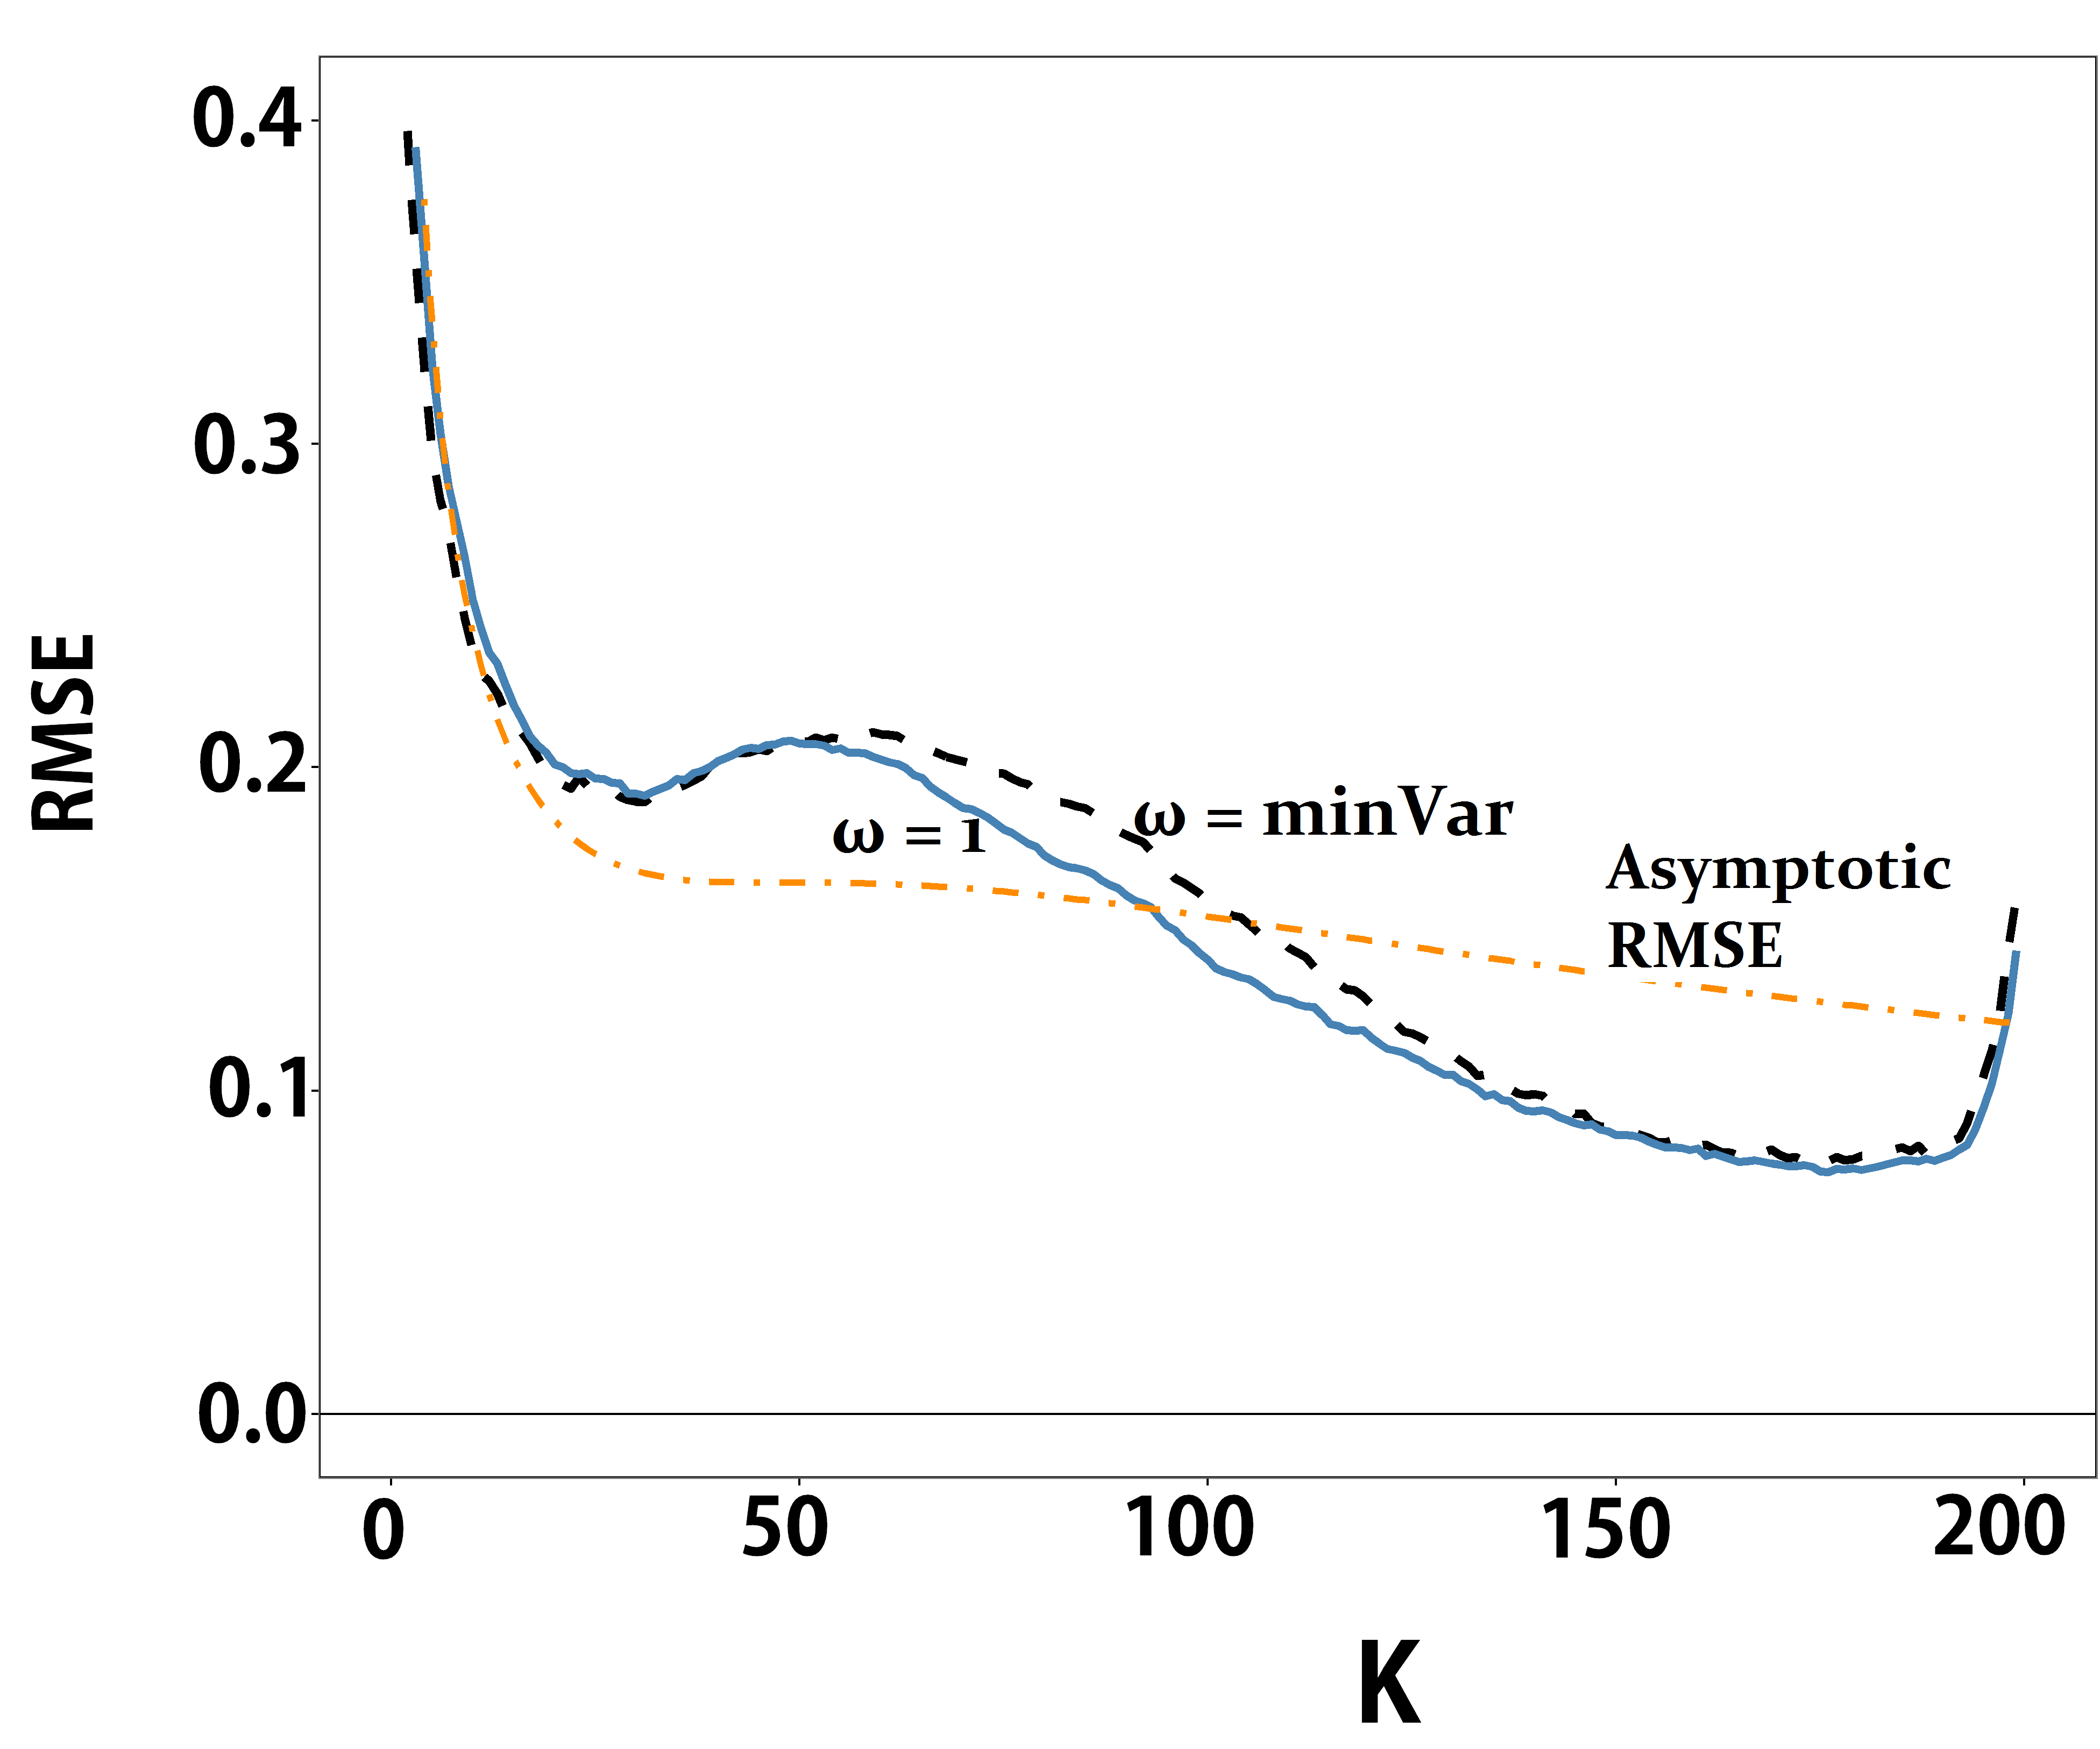
\includegraphics[width=65mm]{./plots/paper1/mseBurrKappa.png}
		\end{subfigure}
		\caption{Bias (left) and root mean squared error (right) in case of the \textbf{Fr\'echet distribution} with $\gamma=0.5$ (top) and Burr distribution with $\gamma=0.75$ (bottom) for sample size $n=200$ comparing  the penalised ML estimator $\hat{\gamma}^P_{k}(1)$ with $\omega=1$, $\omega = \omega_{mv}$ from \eqref{minvar}, and the optimal asymptotic RMSE from \eqref{xisqdiff} replacing $\lambda$ by $C_a\sqrt{k}(k/n)^{-\rho}$.}
		\label{paper1:fig5}
	\end{figure}

In order to illustrate the use of the proposed method we consider the Secura Belgian Re data introduced in section 6.2 in \cite{sts626}.  For $k \leq 100$ the penalised ML estimator $\hat{\gamma}^P_{k}(1)$ is quite constant and follows the Hill estimator quite closely. This is in contrast with the EPD-ML estimates which vary a lot in that region. The Bayesian estimates $\hat{\gamma}^B_{k}(1)$ and CH estimates show somewhat lower estimates. \cite{sts626} concluded that the Hill estimate in this $k$-region is an appropriate choice and the adaptive choice $\hat{k}=98$ was proposed as one of the largest $k$-values in this region. This proposal is also supported by the present analysis, leading to an estimate $\hat{\gamma}^P(1)=0.28$. 
\begin{figure}[h]
	\centering
	\begin{subfigure}[h]{0.45\textwidth}
		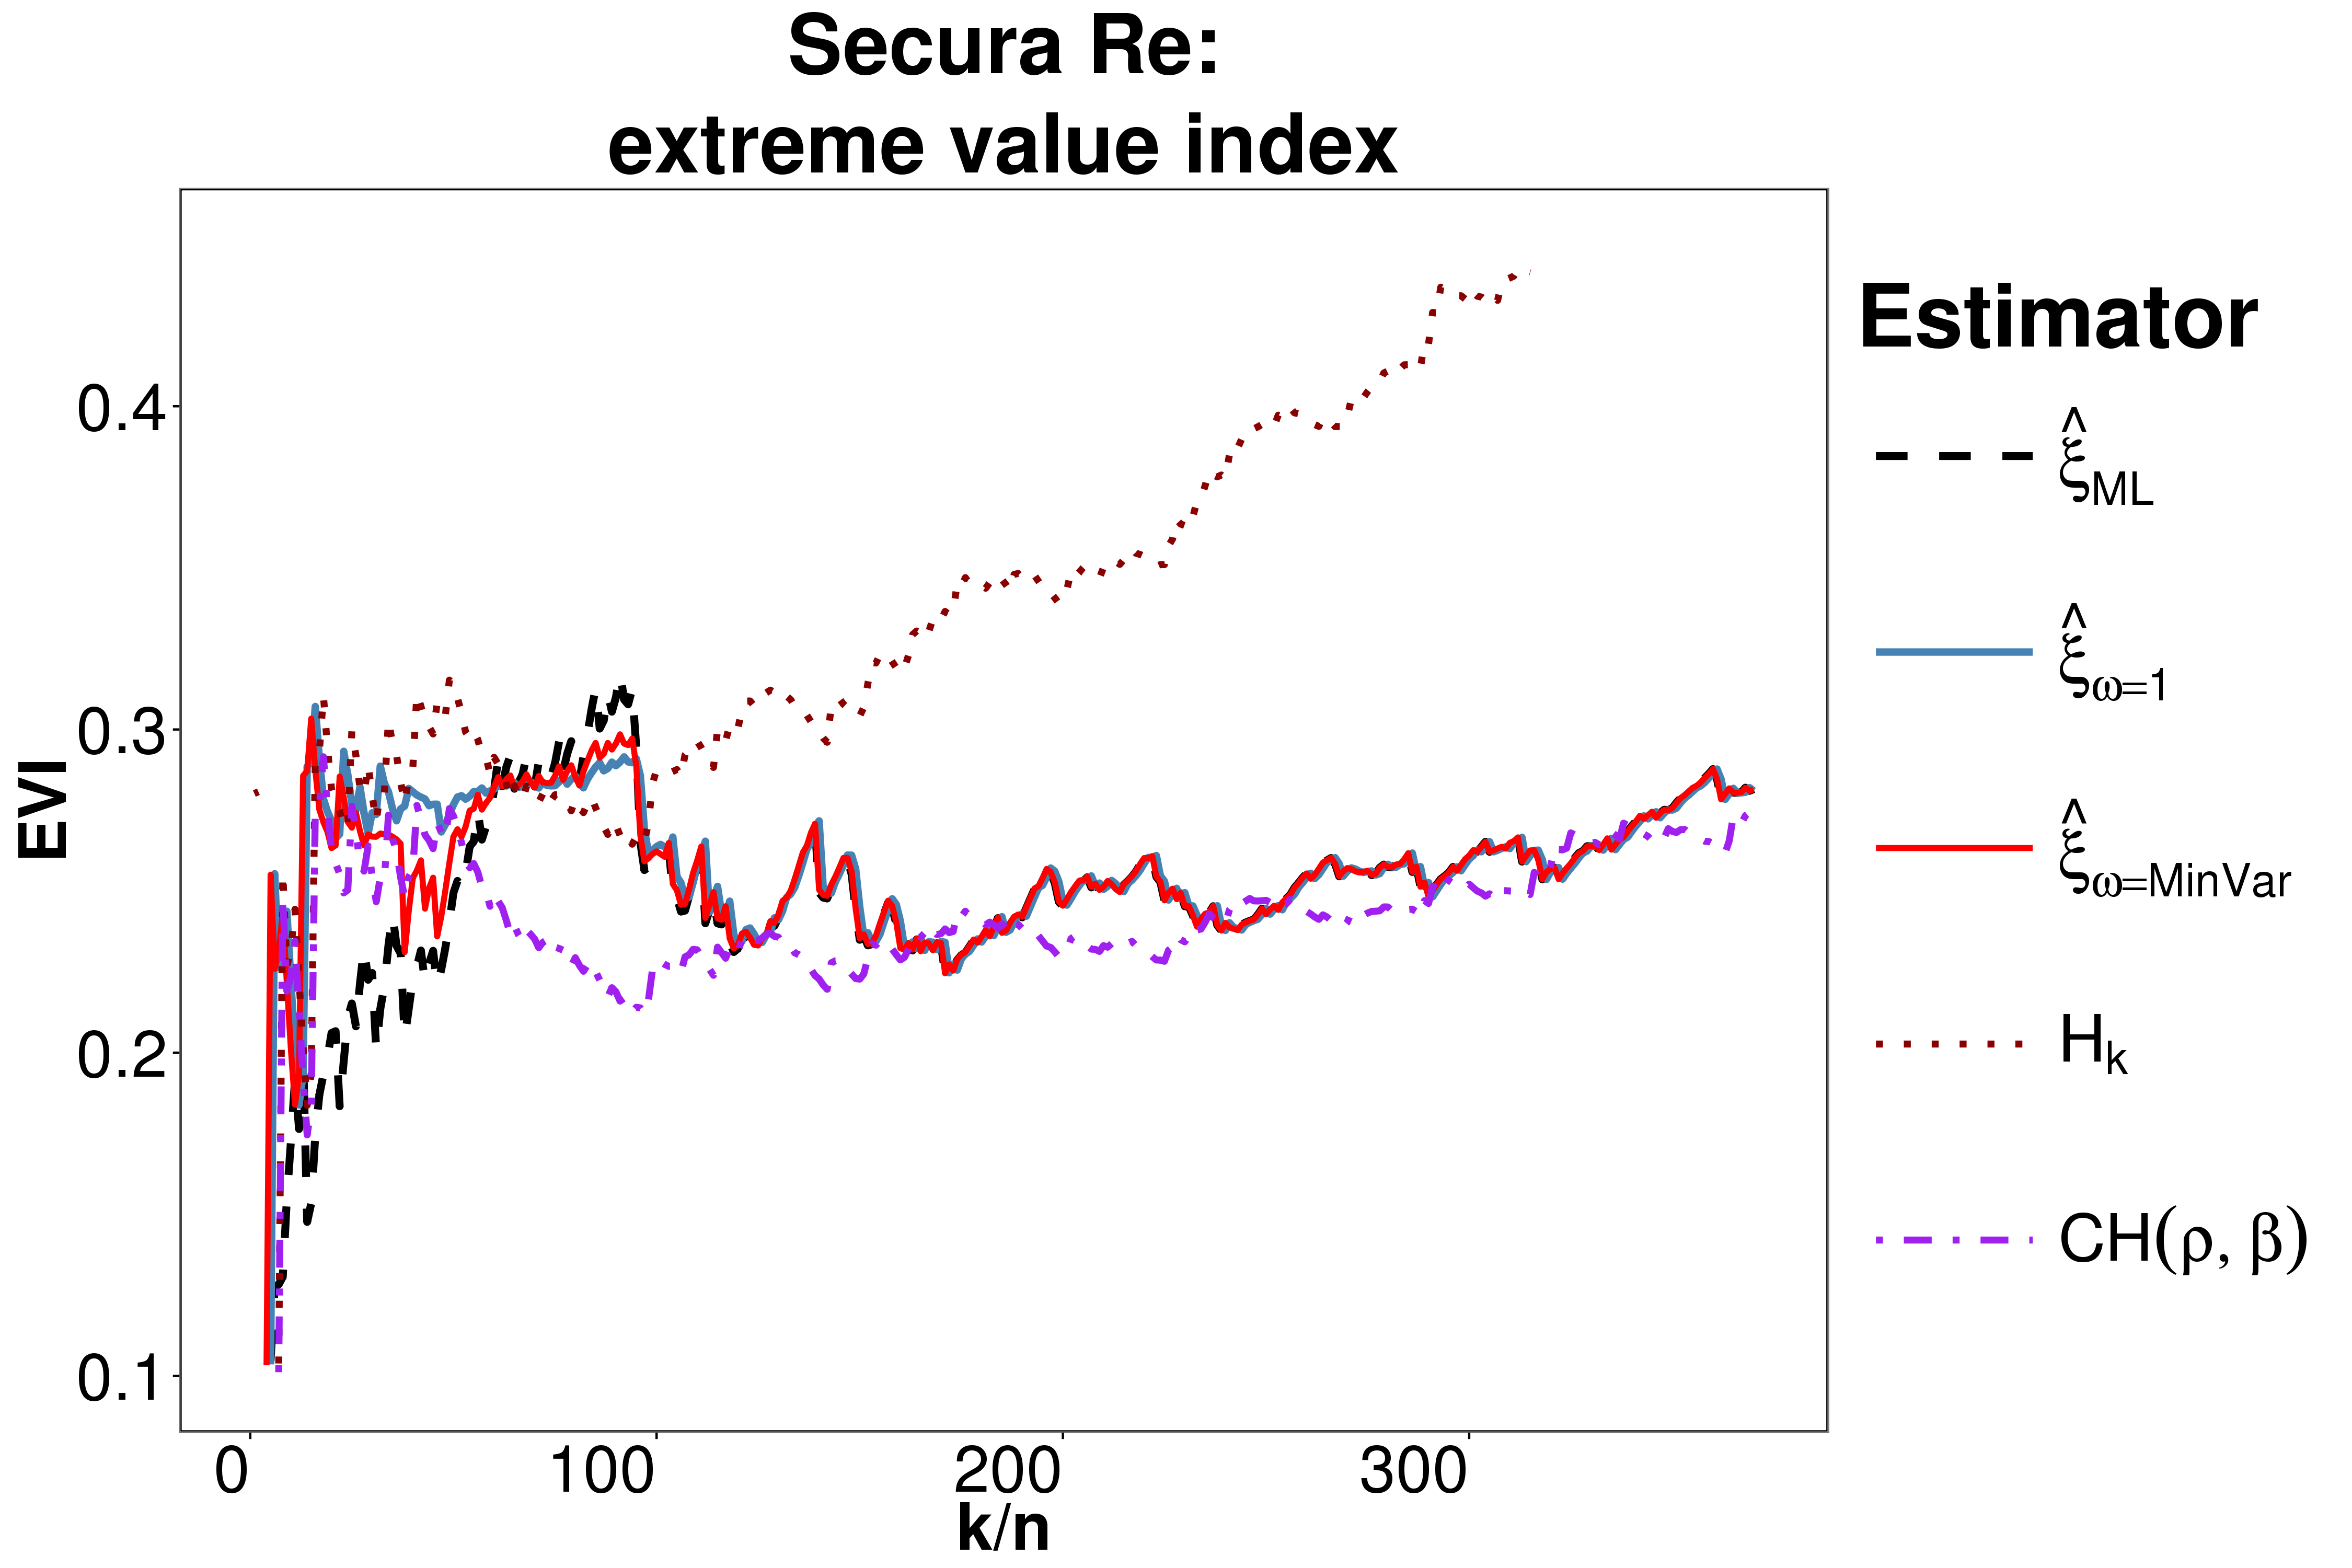
\includegraphics[width=\textwidth]{./plots/paper1/SecuraEVI.png}
	\end{subfigure}
	\hspace{\fill}
	\begin{subfigure}[h]{0.45\textwidth}
		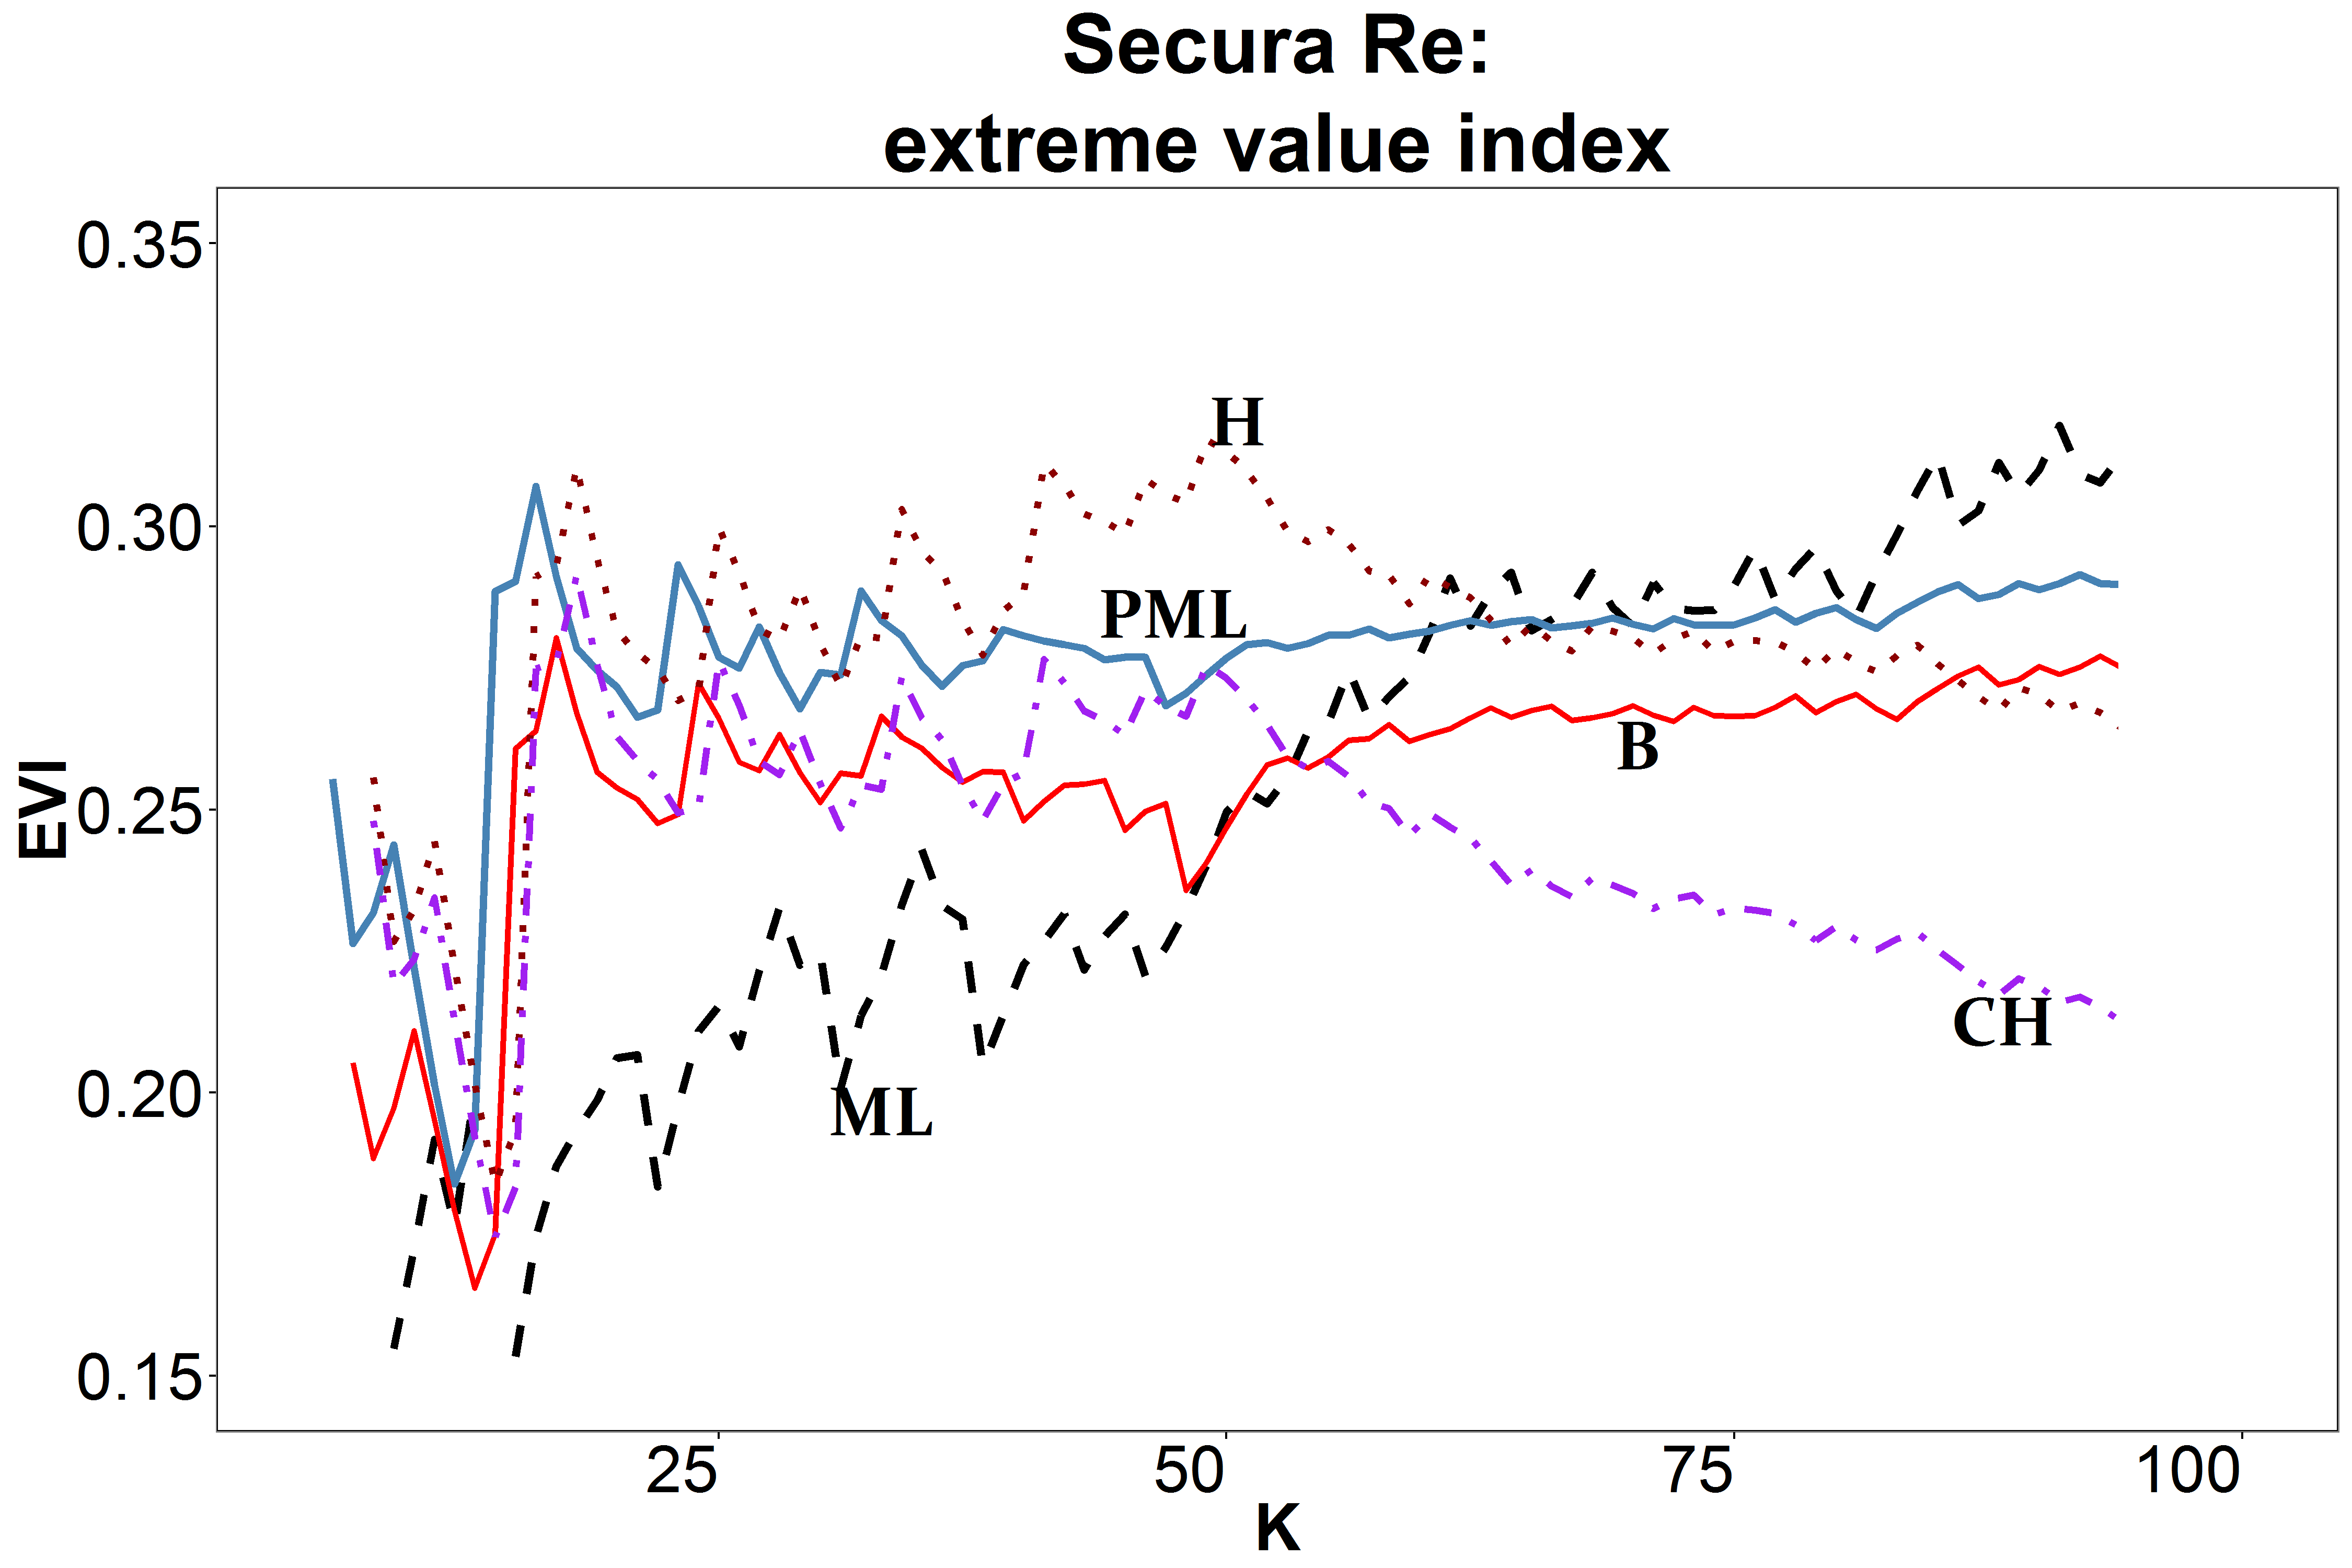
\includegraphics[width=\textwidth]{./plots/paper1/cutSecuraEVI.png}
	\end{subfigure}
	\caption{\footnotesize Estimates of  $\gamma$ for Secura Belgian Re data set: results for the Hill estimator (H), the EPD-ML estimator $\hat{\gamma}_{k}^{ML}$ (ML), the penalised ML estimator $\hat{\gamma}^P_{k}(1)$ with $\omega=1$ (PML), the Bayesian estimator $\hat{\gamma}^B_{k}(1)$ with $\omega=1$ (B), and the minimum variance reduced bias estimator $CH_k$ (CH) (left), focused plot for $k=1,\ldots,100$ (right).}
	\label{Secura} 	
\end{figure}
\\
\section{Chapter conclusion}
We introduced the use of shrinkage estimators in tail estimation, in order to obtain bias reduction jointly with good MSE behaviour. Shrinkage estimators can be obtained through a penalised ML approach, or through a Bayesian implementation. For larger thresholds the proposed estimators follow the behaviour of the classical Hill estimator with small bias and minimal variance, while the new estimators are never worse than the corresponding bias reduced ML estimators without penalisation. The simulated MSE results are competitive with those of other bias reduced estimators. In contrast to existing minimum variance bias reduced estimators we only use second order slow variation conditions.

\begin{subappendices}
\section{Derivation of the expressions of ($\gammab,\db$).} 
First consider the asymptotic approximations of the penalised ML estimator of $\gamma$ based on maximisation of \eqref{loglp}. From \eqref{logl}-\eqref{loglp} using expansions in $\delta \to 0$ 
we obtain 
\begin{eqnarray*}
	{1 \over k}\log l_{pen}(\gamma,\delta |{\bf y}) &=& 
	-\left(1+{1 \over k}\right) \log \gamma -{1 \over k}\left(1+\gamma\right) -\left(\frac{1}{\gamma}+1\right){1 \over k}\sum_{j=1}^k\log y_{j,k} \\
	&& -\delta\left({1 \over \gamma} + 1\right){1 \over k}\sum_{j=1}^k (1-y_{j,k}^{\tau})
	+ \delta {1 \over k}\sum_{j=1}^k (1- (1+\tau)y_{j,k}^{\tau})\\
	&&- {\omega \delta^2 \over 2k\sigma_{k,n}^2}
	+\left({\delta^2 \over 2}\right)\left({1  \over \gamma} +1\right){1 \over k}\sum_{j=1}^k (1-y_{j,k}^{\tau})^2
	- {\delta^2 \over 2} {1 \over k}\sum_{j=1}^k (1- (1+\tau)y_{j,k}^{\tau})^2 \\
	&&+ O(\delta^3) + c,
\end{eqnarray*}
where $c$ is a constant only depending on $\sigma_{k,n}^2$ and $\tau$. Note that ${1 \over k}\sum_{j=1}^k\log y_{j,k}=H_{k,n}$. Then the score functions admit the following expansions in $\delta \downarrow 0$ for $j=1,\ldots,k$:
\begin{eqnarray*}
	{\partial \over \partial \gamma}\log l_{pen}(\gamma,\delta |y_{j,k}) &=& -{1 \over \gamma} + {1 \over \gamma^2} \log y_{j,k}
	+{\delta \over \gamma^2}(1-y_{j,k}^{\tau})
	+ O(\delta^2), \\
	{\partial \over \partial \delta}\log l_{pen}(\gamma,\delta |y_{j,k}) &=& -{1 \over \gamma}\left( 1- (1-\gamma\tau) y_{j,k}^{\tau} \right) -{\omega\delta \over k\sigma^2_{k,n}}\\
	&&
	+ {\delta \over \gamma} \left( 1- 2(1-\gamma\tau) y_{j,k}^{\tau} 
	+ (1-2\gamma\tau-\gamma\tau^2) y_{j,k}^{2\tau}\right)+ O(\delta^2).
\end{eqnarray*}

\vspace{0.4cm}\noindent 
{\it Derivation of Theorem \ref{theorem11}.}
Note that as $k,n \to \infty$, $k/n \to 0$ and $\sqrt{k} a(n/k) \to \lambda$, we also have $k\sigma^2_{k,n} \to \lambda^2 C_a^{-2}$. Also as $\sqrt{k} a(n/k) \to \lambda$ we find using
$E_{k,n}(s) \to 1/(1-\gamma s)$ (see Theorem A.1 in Beirlant et al., 2009) that
$$
D^{P}_{k,n} = -{\gamma C_a^2 \over \lambda^2} 
+ {\rho^4 \over \gamma (1-2\rho)(1-\rho)^2} + o_p(1).
$$
Then, proceeding as in the proof of Theorem 3.1 in Beirlant et al. (2009), we obtain with $\Gamma_{k,n} = \sqrt{k}( H_{k,n}-\gamma)$, $\mathbb{E}_{k,n}(s) =\sqrt{k}(E_{k,n}(s)-{1\over 1-\gamma s })$ ($s<0$), that
\begin{eqnarray*}
	\sqrt{k} \left( \gammab-\gamma \right)&=&
	\sqrt{k} \left( H_{k,n}-\gamma - \db {\rho \over 1-\rho} \right) 
	\\
	&=& \Gamma_{k,n}-{\rho \over 1-\rho}\sqrt{k}\db \\
	&=& \Gamma_{k,n}\left(1+ {\rho^2 \over \gamma(1-\rho^2)}
	{1 \over \gamma C_a^2/\lambda^2+ \rho^4/\gamma(1-2\rho)(1-\rho)^2} \right) \\
	&&- {\rho \over \gamma C_a^2/\lambda^2+\rho^4/\gamma(1-2\rho)(1-\rho)^2} \mathbb{E}_{k,n}(\hat\tau) +o_p(1)\\
	&=& \Gamma_{k,n} \left( 1+ {\rho^2 (1-2\rho)\over \zeta +\rho^4}\right) + 
	\mathbb{E}_{k,n}(\hat\tau)\left( {(-\rho)\gamma(1-2\rho)(1-\rho)^2 \over \rho^4 + \zeta }\right)+o_p(1).
\end{eqnarray*} 
Using Theorem A.1 in Beirlant et al. (2009), \eqref{Abias} and \eqref{Avar} follow under $\sqrt{k} a(n/k) \to \lambda$.
\label{appendix1}

\section{Optimal $\omega$ minimising the $MSE_{\infty}$}
$$
MSE_{\infty} = (E_{\infty})^2 + \text{VAR}_{\infty}
$$
\begin{eqnarray*}
E_{\infty} = \dfrac{\lambda \rho \left(\zeta C_a^2 \omega \right)}{(1-\rho ) \left(\zeta C_a^2 \omega +\lambda ^2 \rho ^4\right)}\ ,\ \ 
\text{VAR}_{\infty} = \dfrac{\left(\lambda ^4 \xi ^2 \rho ^8\right) \left(\dfrac{C_a^4 \zeta ^2 \omega ^2}{\lambda ^4 \rho ^8}+\dfrac{2 \zeta C_a^2 \omega }{\lambda ^2 \rho ^4}+\left(\dfrac{1-\rho }{\rho }\right)^2\right)}{\left(\zeta C_a^2 \omega +\lambda ^2 \rho ^4\right)^2}
\end{eqnarray*}

\begin{eqnarray*}
MSE_{\infty}= \dfrac{\left(\lambda ^4 \xi ^2 \rho ^8\right) \left(\dfrac{C_a^4 \zeta ^2 \omega ^2}{\lambda ^4 \rho ^8}+\dfrac{2 \zeta C_a^2 \omega }{\lambda ^2 \rho ^4}+\left(\dfrac{1-\rho }{\rho }\right)^2\right)}{\left(\zeta C_a^2 \omega +\lambda ^2 \rho ^4\right)^2}+\left(\dfrac{\lambda \rho \left(\zeta C_a^2 \omega \right)}{(1-\rho ) \left(\zeta C_a^2 \omega +\lambda ^2 \rho ^4\right)}\right)^2
\end{eqnarray*}

Where $\zeta = \xi^2(1-2\rho)(1-\rho)^2$

\begin{eqnarray*}
\partial_{\omega}(MSE_{\infty})&=&\dfrac{2 C_a^2 \zeta \lambda ^2 \xi ^2 \rho ^4}{\left(C_a^2 \zeta \omega +\lambda ^2 \rho ^4\right)^2}-\dfrac{2 C_a^2 \zeta \lambda ^4 \xi ^2 \rho ^8}{\left(C_a^2 \zeta \omega +\lambda ^2 \rho ^4\right)^3}+\dfrac{4 C_a^2 \zeta \lambda ^4 \xi ^2 \rho ^7}{\left(C_a^2 \zeta \omega +\lambda ^2 \rho ^4\right)^3}\\&-&\dfrac{2 C_a^2 \zeta \lambda ^4 \xi ^2 \rho ^6}{\left(C_a^2 \zeta \omega +\lambda ^2 \rho ^4\right)^3}-\dfrac{2 C_a6 \zeta ^3 \xi ^2 \omega ^2}{\left(C_a^2 \zeta \omega +\lambda ^2 \rho ^4\right)^3}-\dfrac{2 C_a6 \zeta ^3 \lambda ^2 \rho ^2 \omega ^2}{(1-\rho )^2 \left(C_a^2 \zeta \omega +\lambda ^2 \rho ^4\right)^3}\\&-&\dfrac{4 C_a^4 \zeta ^2 \lambda ^2 \xi ^2 \rho ^4 \omega }{\left(C_a^2 \zeta \omega +\lambda ^2 \rho ^4\right)^3}+\dfrac{2 C_a^4 \zeta ^2 \xi ^2 \omega }{\left(C_a^2 \zeta \omega +\lambda ^2 \rho ^4\right)^2}+\dfrac{2 C_a^4 \zeta ^2 \lambda ^2 \rho ^2 \omega }{(1-\rho )^2 \left(C_a^2 \zeta \omega +\lambda ^2 \rho ^4\right)^2}
\end{eqnarray*}

\begin{eqnarray*}
\partial_{\omega}(MSE_{\infty})=&\dfrac{\lambda ^4 \xi ^2 \rho ^8 \left(\dfrac{2 C_a^4 \zeta ^2 \omega }{\lambda ^4 \rho ^8}+\dfrac{2 \zeta C_a^2}{\lambda ^2 \rho ^4}\right)}{\left(\zeta C_a^2 \omega +\lambda ^2 \rho ^4\right)^2}-\dfrac{2 \zeta C_a^2 \lambda ^4 \xi ^2 \rho ^8 \left(\dfrac{C_a^4 \zeta ^2 \omega ^2}{\lambda ^4 \rho ^8}+\dfrac{2 \zeta C_a^2 \omega }{\lambda ^2 \rho ^4}+\dfrac{(1-\rho )^2}{\rho ^2}\right)}{\left(\zeta C_a^2 \omega +\lambda ^2 \rho ^4\right)^3}\\&-\dfrac{2 \zeta C_a^6 \lambda \rho ^2 \omega ^2}{(1-\rho )^2 \left(\zeta C_a^2 \omega +\lambda ^2 \rho ^4\right)^3}+\dfrac{2 \zeta C_a^4 \lambda \rho ^2 \omega }{(1-\rho )^2 \left(\zeta C_a^2 \omega +\lambda ^2 \rho ^4\right)^2}
\end{eqnarray*}

Which simplifies to:
\begin{eqnarray*}
=\dfrac{2 C_a^2 \zeta \lambda ^4 \xi ^2 (2 \rho -1) \rho ^6}{\left(C_a^2 \zeta \omega +\lambda ^2 \rho ^4\right)^3}+\dfrac{2 C_a^4 \zeta ^2 \lambda ^4 \rho ^6 \omega }{(\rho -1)^2 \left(C_a^2 \zeta \omega +\lambda ^2 \rho ^4\right)^3}
\end{eqnarray*}

\begin{eqnarray*}
=\dfrac{2 C_a^2 \zeta \lambda ^4 \rho ^6 \left(C_a^2 \zeta \omega +\xi ^2 (\rho -1)^2 (2 \rho -1)\right)}{(\rho -1)^2 \left(C_a^2 \zeta \omega +\lambda ^2 \rho ^4\right)^3}
\end{eqnarray*}

Set $\partial_{\omega}(MSE_{\infty})=0$ and solve for $\omega$
\begin{eqnarray*}
\omega \to C_a^{-2}*\left(-\dfrac{\xi ^2 (\rho -1)^2 (2 \rho -1)}{\zeta }\right)
\end{eqnarray*}

After substituting $\zeta$ back into the equation we get:
\begin{eqnarray*}
\omega = C_a^{-2} * \left(-\dfrac{(\rho -1)^2 (2 \rho -1)}{(1-2 \rho ) (1-\rho )^2}\right) = C_a^{-2}
\end{eqnarray*}

\begin{eqnarray*}
\partial_{\omega}^2(MSE_{\infty})=&
\dfrac{2 C_a^4 \zeta ^2 \lambda ^4 \rho ^6}{(\rho -1)^2 \left(C_a^2 \zeta \omega +\lambda ^2 \rho ^4\right)^3}-\dfrac{6 C_a^4 \zeta ^2 \lambda ^4 \rho ^6 \left(C_a^2 \zeta \omega +\xi ^2 (\rho -1)^2 (2 \rho -1)\right)}{(\rho -1)^2 \left(C_a^2 \zeta \omega +\lambda ^2 \rho ^4\right)^4}
\end{eqnarray*}

Substituting $\zeta$ and $\omega= C_a^{-2}$ into the equation:

\begin{eqnarray*}
\partial_{\omega}^2(MSE_{\infty})=&&-\dfrac{8 C_a^4 \lambda ^4 \xi ^4 \rho ^{10}}{\left(\xi ^2 (\rho -1)^2 (2 \rho -1)-\lambda ^2 \rho ^4\right)^3}+\dfrac{24 C_a^4 \lambda ^4 \xi ^4 \rho ^9}{\left(\xi ^2 (\rho -1)^2 (2 \rho -1)-\lambda ^2 \rho ^4\right)^3}\\&-&\dfrac{26 C_a^4 \lambda ^4 \xi ^4 \rho ^8}{\left(\xi ^2 (\rho -1)^2 (2 \rho -1)-\lambda ^2 \rho ^4\right)^3}+\dfrac{12 C_a^4 \lambda ^4 \xi ^4 \rho ^7}{\left(\xi ^2 (\rho -1)^2 (2 \rho -1)-\lambda ^2 \rho ^4\right)^3}\\&-&\dfrac{2 C_a^4 \lambda ^4 \xi ^4 \rho ^6}{\left(\xi ^2 (\rho -1)^2 (2 \rho -1)-\lambda ^2 \rho ^4\right)^3}
\end{eqnarray*}

\begin{eqnarray*}
=&&\dfrac{2 C_a^4 \lambda ^4 \xi ^4 (1-2 \rho )^2 (1-\rho )^4 \rho ^6}{(\rho -1)^2 \left(C_a^2 \xi ^2 (1-\rho )^2 (1-2 \rho ) \omega +\lambda ^2 \rho ^4\right)^3}\\&-&\dfrac{6 C_a^4 \lambda ^4 \xi ^4 (1-2 \rho )^2 (1-\rho )^4 \rho ^6 \left(C_a^2 \xi ^2 (1-2 \rho ) (1-\rho )^2 \omega +\xi ^2 (\rho -1)^2 (2 \rho -1)\right)}{(\rho -1)^2 \left(C_a^2 \xi ^2 (1-\rho )^2 (1-2 \rho ) \omega +\lambda ^2 \rho ^4\right)^4}
\end{eqnarray*}

\begin{eqnarray*}
=&&-\dfrac{2 C_a^4 \lambda ^4 \xi ^4 (1-2 \rho )^2 (\rho -1)^2 \rho ^6}{\left(\xi ^2 (\rho -1)^2 (2 \rho -1)-\lambda ^2 \rho ^4\right)^3}
\end{eqnarray*}

This leads to the following series expansion around zero
\begin{eqnarray*}
&-\dfrac{2 \lambda ^4 \left(C_a^4 \rho ^6\right)}{\xi ^2 (\rho -1)^4 (2 \rho -1)}+O\left(\lambda ^5\right) \\&\approx
\dfrac{2 C_a^4 \lambda ^4 \rho ^6}{\xi ^2 (\rho -1)^4 (1-2 \rho)} > 0
\end{eqnarray*}Using the fact that $\rho < 0$, we can conclude that $\omega = C_a^{-2}$ is the optimal value that minimises the MSE.
\label{appendix1a}
\newpage
\section{Algorithm to estimate $\rho$}
	In this section we provide the algorithm of \cite{alves2003new} used to estimate $\rho$.
	\begin{enumerate}
			\item Given a sample ($X_1,X_2,...,X_n$), plot the estimates of \begin{equation}\label{pkt}
			\hat{\rho}_{k,r}:=\min\{0,\dfrac{3(T^{(\tau)}_{k,n}-1)}{T^{(\tau)}_{k,n}-3}\},
			\end{equation}for $\tau=0$, where 
			\begin{equation}\label{tau0}
			T_{k,n}:= \dfrac{\left(M_{k,n}^{(1)}\right)^{\tau}-\left(\dfrac{M^{(2)}_{k,n}}{2}\right)^{\tau/2}}{\left(\dfrac{M^{(2)}_{k,n}}{2}\right)^{\tau/2}-\left(\dfrac{M^{(3)}_{k,n}}{6}\right)^{\tau/3}}
			\end{equation}and
			\begin{equation}
			M^{(j)}_{k,n}:=\dfrac{1}{k}\sum_{i\leq k}^{}(\log X_{n-i+1:n}-\log X_{n-k:n})^j, \ \ j \geq 1.
			\end{equation}since $\tau=0$, the notation $a^{b\tau}=b\ln a$ is used and therefore \autoref{tau0} is written as
			\begin{equation}
			T_{k,n}:= \dfrac{\log(M_{k,n}^{(1)})-\dfrac{1}{2}\log\left(\dfrac{M^{(2)}_{k,n}}{2}\right)}{\dfrac{1}{2}\log\left(\dfrac{M^{(2)}_{k,n}}{2}\right)-\dfrac{1}{3}\log\left(\dfrac{M^{(3)}_{k,n}}{6}\right)}
			\end{equation}
			
			\item Consider $\{\hat{\rho}_{k,n}\}_{k\in \mathcal{K}}$ as given in \autoref{pkt} for large $k$, say $k\in \mathcal{K}=([n^{0.990}],[n^{0.999}])$, compute their median, denoted $\rho_\tau$ and work with $\hat{\rho}\equiv\hat{\rho}_{\tau_{0}}:=\hat{\rho}_{k_1}$, with\begin{equation}
			k_1=[n^{0.995}]
			\end{equation}
		\end{enumerate}
		The choice of the level $k_1$ is not very important, we can consider any reasonably large value of $k$ of order $n^{1-\epsilon}$ from some intermediate sequence of integers $k=k(n)$ satisfying $\lim\limits_{n\rightarrow\infty}\sqrt{k}A(n/k)=\infty$. This estimator uses more upper order statistics than the first order parameter $\gamma$.
\label{appendix1b}
\end{subappendices}
\chapter{Penalised Bias Reduction in Extreme Value Estimation for Censored Pareto-type Data}\label{chap4}
\setcounter{equation}{0}
\href{https://www.sciencedirect.com/science/article/pii/S0167668717302573}{\textit{This chapter is based on Beirlant, J., Maribe, G. and Verster, A., 2018. Penalized bias reduction in extreme value estimation for censored Pareto-type data, and long-tailed insurance applications. Insurance: Mathematics and Economics, 78, pp.114-122.}}

\section{Introduction} % --- sections in UPPERCASE
\label{Sec1}       % --- this section label
Extreme value analysis under random right censoring is becoming more popular with applications for example in survival analysis, reliability and insurance. For instance, in certain long-tailed insurance products, such as car liability insurance, long developments of claims are encountered. At evaluation of the portfolio a large proportion of the claims are then not fully developed and hence are censored.

\vspace{0.3cm}
In the setting of random right censoring the variable of interest $X$ with CDF $F$ can be censored by a random variable $C$ with CDF $G$. Moreover observations of $X$ and $C$ are assumed to be independent. One then observes $Z=\min (X,C)$ with CDF $H$ satisfying 
$1-H=(1-F)(1-G)$, jointly with the indicator $\Delta =1_{(X \leq C)}$ which equals 1 if the observation $Z$ is non-censored. Here we assume that $X$ and $C$ both are Pareto-type distributed with EVI $\gamma_1 >0$ and $\gamma_2 >0$, i.e. 
\[
\bar{F} (x) = 1-F(x) = x^{-1/\gamma_1}\ell_1 (x) \mbox{ and } \bar{G}(y) = 1-G(y) = y^{-1/\gamma_2}\ell_2 (y), \;\; x,y>1,
\]
where both $\ell_1, \ell_2$ are slowly varying at infinity:
\[
\ell_j(tx)/\ell_j (t) \to_{t \to \infty} 1, \;\; \mbox{ for every } x>1 \;\; (j=1,2).
\]
Note that $1-H$ then also belongs to the domain of attraction of an extreme value distribution with positive EVI $\gamma = { {\gamma_1 \gamma_2}\over{\gamma_1+\gamma_2}}$.
Of course, the smaller $\gamma_2/\gamma_1$ the heavier the censoring will be. In long-tailed insurance applications as discussed above, the proportion of censored data can well be larger than 50\%, so that the situation $\gamma_2 < \gamma_1$ is then most relevant.

\vspace{0.3cm}
In this section we discuss the estimation of $\gamma_1$ based on IID observations $(Z_i,\Delta_i)$ ($i=1,\ldots,n$) with $Z_i =\min (X_i,C_i)$ and $\Delta_i=1_{(X_i\leq C_i)}$, where $(X_i,C_i)$ ($i=1,\ldots,n$) are IID. random variables from $(F,G)$. In the next section we review the available estimators for $\gamma_1$ that were published in the literature. In \autoref{chap4::Sec3} we propose a new bias reduced estimator which is based on an estimator proposed by \cite{worms2014new}. Moreover we show how shrinkage estimation, as introduced in \cite{beirlant2017using} in the non-censoring case, can also be used in the censoring context. In \autoref{chap4::SecB} a parametric bootstrap algorithm is proposed in order to construct confidence intervals for $\gamma_1$. We then report on a simulation study involving all available estimators and the proposed bootstrap algorithm. Finally we make a detailed study of a motor third party liability (MTPL) case study.

\section{A review of estimators of $\gamma_1$}
\label{Sec2}

In case there is no censoring (i.e. $\gamma_2 =\infty$ and $1-H=1-F$), the \cite{hill1975simple} estimator is the benchmark estimator for $\gamma_1=\gamma$. Denoting the ordered $Z$ data by $Z_{1,n}\leq Z_{2,n}
\leq \ldots \leq Z_{n,n}$ this estimator is given by
\[
\hat{\gamma}_{Z,k}^H= {1 \over k}\sum_{j=1}^k \log {Z_{n-j+1,n} \over Z_{n-k,n}}.
\]
This estimator follows using maximum likelihood when approximating the distribution of the peaks $Z/t$ over a threshold $t$, given $Z> t$, by a simple Pareto distribution with density $y \mapsto \gamma^{-1} y^{-\gamma^{-1}-1}$, and taking a top order statistic $Z_{n-k,n}$ as a threshold $t$. \\
It can also be found back by estimating the functional
\begin{equation}
L_t := \mathbb{E}(\log Z - \log t|Z>t)= \int_1^{\infty} {\bar{F}(ut) \over \bar{F}(t)} {du \over u}, 
\label{MElog}
\end{equation}
which tends to the EVI $\gamma$ of $Z$ as $t\to \infty$. In \eqref{MElog}
$\bar{F}$ is estimated by the empirical survival function $1-\hat{F}_n$, again using $Z_{n-k,n}$ as a threshold $t$. This leads to an alternative writing of $\hat{\gamma}_{Z,k}^H$ by partial summation:
\[
\hat{\gamma}_{Z,k}^{(H)}= {1 \over k}\sum_{j=1}^k j(\log Z_{n-j+1,n} - \log Z_{n-j,n}).
\]

\vspace{0.3cm}
While both approaches yield the same estimator in the non-censoring case this is no longer the case under random censoring. 
\begin{itemize}
\item
\cite{beirlant2007estimation} proposed the following estimator of $\gamma_1$ using the maximum likelihood approach:
\begin {equation}
\hat{\gamma}_{1,k}^{(H)} = {\hat{\gamma}_{Z,k}^{(H)} \over \hat{p}_k} ,
\label{Censored Hill}
\end {equation} 
with $\hat{p}_k = {1\over k} \sum_{j = 1}^k \Delta_{n-j+1,n}$ the proportion of non-censored observations under the largest $k$ observations of $Z$, where $\Delta_{n-j+1,n}$ denotes the $\Delta$ indicator attached to $Z_{n-j+1,n}$ $(1 \leq j \leq n)$. Indeed, $\hat{\gamma}_{Z,k}^H$ estimates $\gamma$ while $\hat{p}_k$ is shown to be a consistent estimator of $p=\gamma_2/(\gamma_1+\gamma_2)$. Einmahl et al. (2008) enhanced the asymptotic analysis of this estimator and generalised this approach by considering any classical EVI estimator $\hat{\gamma}_{Z,k}^{(.)}$ of $\gamma$, proposing the estimators 
$
\hat{\gamma}_{1,k}^{(.)}={\hat{\gamma}_{Z,k}^{(.)}\over \hat{p}_k}$.
See also \cite{gomes2003censoring}, \cite{gomes2011estimation}, and \cite{brahimi2015gaussian} for other papers in this spirit. 
\item
\cite{worms2014new} essentially used the second approach estimating \eqref{MElog} by substituting $1-F$ with the Kaplan-Meier estimator $$1-\hat{F}^{KM}_n (x) = \Pi_{Z_{i,n} \leq x} \left(1- {1 \over n-i+1} \right)^{\Delta_{i,n}}$$, setting $1-\hat{F}^{KM}_n (Z_{n,n})=0$: 
\begin {equation}
\hat{\gamma}_{1,k}^{(W)} = \sum_{j=1}^k {1-\hat{F}^{KM}_n (Z_{n-j+1,n}) \over 1-\hat{F}^{KM}_n (Z_{n-k,n})} \left( \log Z_{n-j+1,n}-\log Z_{n-j,n}\right).
\label{Worms}
\end {equation}
\cite{worms2014new} also introduced 
\begin {equation}
\hat{\gamma}_{1,k}^{(KM)} = \sum_{j=1}^k {1-\hat{F}^{KM}_n (Z_{n-j+1,n}) \over 1-\hat{F}^{KM}_n (Z_{n-k,n})}{\Delta_{n-j+1,n} \over j} \left( \log Z_{n-j+1,n}-\log Z_{n-k,n}\right).
\label{WormsKM}
\end {equation}
Through simulations the estimator $\hat{\gamma}^{(W)}_{1,k}$ was found to have the best RMSE behaviour for smaller values of $k$. Below we will then concentrate on $\hat{\gamma}_{1,k}^{(W)}$. Unfortunately, the asymptotic distribution of $\hat{\gamma}_{1,k}^{(W)}$ is not known up to now. The asymptotic normality of a fixed threshold version of $\hat{\gamma}_{1,k}^{(KM)}$ can be derived from \cite{worms2018extreme} in case $\gamma_1 < \gamma_2$. \cite{brahimi2015nelson} consider closely related estimators but also considered asymptotic results in case $\gamma_1 < \gamma_2$ or $p >1/2$. 
\item
In an objective Bayesian approach \citep[see][]{zellner1971introduction}, \cite{ameraoui2016bayesian} recently proposed several other estimators. They considered the maximum posterior (m) and the mean posterior (e) estimators of the posterior density of $\gamma_1$. The maximal data information (M) prior and a conjugate gamma prior with parameters $(a,b)$ were considered. It was also shown that Jeffreys prior lead to special cases of the conjugate prior estimators setting $a=b=0$. This then leads to the following estimators:
\begin{eqnarray}
\hat{\gamma}_{1,k}^{(m,M)}&=&{2 k\hat{\gamma}_{Z,k}^{(H)} \over 1+k\hat{p}_k+\sqrt{(1+k\hat{p}_k)^2+4k\hat{\gamma}_{Z,k}^{(H)}}} , \label{Bayes1} \\
\hat{\gamma}_{1,k}^{(e,a,b)} &=& {k\hat{\gamma}_{Z,k}^{(H)}+b \over k\hat{p}_k +a},
\label{Bayes2} \\
\hat{\gamma}_{1,k}^{(m,a,b)} &=& {k\hat{\gamma}_{Z,k}^{(H)}+b \over k\hat{p}_k +a-1}.
\label{Bayes3}
\end{eqnarray}
\end{itemize}

\vspace{0.3cm}
It is well-known that extreme value estimators often suffer from severe bias. In the random censoring case \cite{einmahl2008statistics} first derived the asymptotic bias of $\hat{\gamma}_{1,k}^{(H)}$, which was further detailed in \cite{beirlant2016bias} under more specific assumptions on the slowly varying functions $\ell_1 $ and $\ell_2$, which are commonly proposed in EVT:
\begin{eqnarray*}
1-F(x)&=&C_1 {x^{-1/\gamma_1}}(1+D_{1} x^{-\beta_1} (1+o(1))),\; x \to \infty,\\
%\label{Second order 1}
1-G(y)&=&C_2 {y^{-1/\gamma_2}}(1+D_{2} x^{-\beta_2} (1+o(1))),\; y \to \infty,
%\label{Second order 2}
\end{eqnarray*}
where $\beta_1,\beta_2,C_1,C_2$ are positive constants and $D_1,D_2$ are real constants. Taking the bias of the Hill estimator $\hat{\gamma}^{(H)}_{Z,k}$ as a reference, it was observed that especially when $\beta_1 \leq \beta_2$ the bias of $\hat{\gamma}_{1,k}^{(H)}$ increases with decreasing value of $p$, i.e. for smaller $\gamma_2/\gamma_1$.
Within the maximum likelihood approach, a bias reduced estimator was then proposed for the censoring case following the technique from \cite{beirlant2009second} where the distribution of the excesses $X/t|X>t$ is approximated by the EPD with CDF
$\mathbb{P}(Y \leq y)=1-(y\{1+\delta_t (1-y^{-\beta_1})\})^{-1/\gamma_1}$ where $\delta_t = \gamma_1 D_1 t^{-\beta_1} (1+o(1))$ as $t \to \infty$. The resulting estimator is given by
\begin{equation}
\hat{\gamma}_{1,k}^{(EP)}
=\hat{\gamma}_{1,k}^{(H)}+C_{\hat{\gamma}_{1,k}^{(H)},\beta_*}{H_{Z,k}^{(-\beta_*)}\over \hat{p}_k}
\left\{
H_{Z,k}^{(-\beta_*)}-\hat{\gamma}_{1,k}^{(H)}E_{Z,k}^{(c)}(-\beta_*)
\right\}
\label{biasreduced}
\end{equation}
where, $\beta_{*}=\min(\beta_1,\beta_2)$ and  
\begin{eqnarray*}
H_{Z,k}^{(-\beta_*)}&=&{1\over\beta_*}
\left(1-{1\over{k}}\sum_{j=1}^k \left({Z_{n-j+1,n}\over Z_{n-k,n}}\right)^{-\beta_*}\right), \\
E_{Z,k}^{(c)}(-\beta_*)&=&{1\over{k}}\sum_{j=1}^k \Delta_{n-j+1,n}{\left(Z_{n-j+1,n}\over{Z_{n-k,n}}\right)}^{-\beta_*},\\ C_{\gamma,\beta_*}&=&-{{(1+\gamma\beta_*)^3(1+2\gamma\beta_*)}\over{\gamma^4\beta_*^3}}.
\end{eqnarray*}
In this estimation procedure $\beta_*$ is assumed to be known. In fact, since in the definition of the EP distribution the term $y^{-\beta_*}$ is multiplied by the $\delta_t$-factor, the asymptotic distribution of tail estimators based on the EP distribution will not depend on the asymptotic distribution of an estimator of $\beta_*$. One can also impute estimators of the parameter $\beta_*$ of the distribution $H$ of $Z$ without increasing the bias in estimating $\gamma_1$. Estimators of $\rho_* = -\gamma \, \beta_*$ were discussed in \cite{alves2003new}. An estimator for $\beta_*$ is then given by $-\rho_*/ \hat{\gamma}_{Z,k}^{(H)}$. In the simulations the sensitivity of the choice of $\rho_*$ was examined.
In \eqref{biasreduced} one can reparametrize $\beta_* \hat{\gamma}_{Z,k}^{(H)}$ by $-\rho_*$ with $\rho_* <0$, leading to
\begin{equation}
\hat{\gamma}_{1,k}^{(EP)}(\rho_*)=
\hat{\gamma}_{1,k}^{(H)}- 
{\hat{\gamma}_{1,k}^{(H)} (1-\rho_*)^2(1-2\rho_*)\over \rho_*^3}
\left\{
H_{Z,k}^{(\rho_*/ \hat{\gamma}_{Z,k}^{(H)})}-\hat{\gamma}_{1,k}^{(H)}E_{Z,k}^{(c)}(\rho_*/ \hat{\gamma}_{Z,k}^{(H)})
 \right\}.
\label{EPrho}
\end{equation}
It was shown that when using the correct value of $\beta_*$ or $\rho_*$, the asymptotic bias of $\hat{\gamma}_{1,k}^{(EP)}$ is 0 as long as $\sqrt{k} (k/n)^{\beta_*} = O(1)$, whereas the asymptotic bias of the original estimator $\hat{\gamma}^{(H)}_{1,k}$ is only 0 when $\sqrt{k} (k/n)^{\beta_*} \to 0$ as $k,n \to \infty$. Hence the bias is reduced for a longer set of values of $k \geq 1$ when choosing $t$ as $X_{n-k,n}$. At the other hand the variance of this bias reduced estimator was shown to be increased by the factor $\left({1+\gamma\beta_*\over \gamma \beta_*} \right)^2$ in comparison with the estimator $\hat{\gamma}^{(H)}_{1,k}$.

\vspace{0.3cm}
Before comparing the different estimators through simulations, we next derive a bias reduced estimator starting from the Worms \& Worms estimator $\hat{\gamma}_{1,k}^{(W)}$ from \eqref{Worms}. Following \cite{beirlant2017using}, we then also apply shrinkage estimation on $\delta_t$ forcing this parameter to decrease to $0$ as $t \to \infty$ or $k \downarrow 1$ as it is the case in the mathematical definition of $\delta_t$.

\section{Bias reduction of the Worms \& Worms estimator and penalised estimation of bias } 
\label{chap4::Sec3}

Using the EP approximation to the survival function ${\bar{F}(ut) \over \bar{F}(t)} $ of the excesses $X/t|X>t$, leads to the following approximation of the integral expression of $L_t$ in \eqref{MElog}: as $t\to \infty$
\begin{equation}
L_t = \int_1^{\infty} {\bar{F}(ut) \over \bar{F}(t)} {du \over u} = \gamma_1 - \delta_t {\beta_1 \gamma_1 \over 1+\beta_1 \gamma_1}(1+o(1)).
\label{Lt}
\end{equation}
Similarly, considering 
$$E_t (-\beta_1):= \mathbb{E} \left( ({X \over t})^{-\beta_1}|X>t \right) = 1+ \int_1^{\infty}{\bar{F}(ut) \over \bar{F}(t)}
du^{-\beta_1}$$ leads to 
\begin{equation}
(1+\gamma_1\beta_1) E_t (-\beta_1) = 1 + {\delta_t \over \gamma_1} {(\beta_1 \gamma_1)^2 \over 1+2\beta_1 \gamma_1}(1+o(1)),\ \ \ \ t \rightarrow \infty.
\label{Et}
\end{equation}
Substituting $\gamma_1$ in the left hand side of \eqref{Et} by
the expression $L_t + \delta_t {\beta_1 \gamma_1 \over 1+\beta_1 \gamma_1}$ which follows from \eqref{Lt}, one obtains for $t \to \infty$ that
\begin{eqnarray*}
&& \hspace{-1cm}(1+\beta_1 L_t) E_t(-\beta_1) \\&=& 1+ \left\{ {\delta_t \over \gamma_1}
{(\beta_1 \gamma_1)^2 \over 1+2\beta_1 \gamma_1}- \delta_t {\beta_1^2 \gamma_1 \over 1+\beta_1 \gamma_1}E_t(-\beta_1)\right\} (1+o(1))\\
&=& 1+ {\delta_t \over \gamma_1}(\beta_1 \gamma_1)^2 [{1 \over 1+2\beta_1\gamma_1}-{1 \over (1+\beta_1\gamma_1)^2}](1+o(1))\\
&=& 1+ {\delta_t \over \gamma_1}{ (\beta_1 \gamma_1)^4 \over (1+\beta_1\gamma_1)^2(1+2\beta_1\gamma_1)}(1+o(1)),
\end{eqnarray*} 
where in the second step we approximated $E_t(-\beta_1)$ by $(1+\gamma_1\beta_1)^{-1}$. We now conclude that 
\begin{equation}
\delta_t = {L_t (1+\beta_1 L_t)^3(1+2\beta_1 L_t) \over (\beta_1 L_t)^4}\left\{E_t(-\beta_1)-{1 \over 1+\beta_1 L_t} \right\}(1+o(1)).
\label{deltatilde}
\end{equation}
Estimating $L_t$ at a random threshold $Z_{n-k,n}$ by $\hat{\gamma}_{1,k}^{(W)}$ and similarly $E_t(-\beta_1)$ by
\[
\hat{E}_k (-\beta_1)= 1+ \sum_{j=1}^k {1-\hat{F}^{KM}_n (Z_{n-j+1,n}) \over 1-\hat{F}^{KM}_n (Z_{n-k,n})} 
\left( Z^{-\beta_1}_{n-j+1,n}- Z_{n-j,n}^{-\beta_1} \right)/Z^{-\beta_1}_{n-k,n},
\]
we obtain the following bias reduced estimator for $\gamma_1$ combining \eqref{Lt} and \eqref{deltatilde}:
\begin{equation}
\hat{\gamma}_{1,k}^{(BR,W)}=
\hat{\gamma}_{1,k}^{(W)}+ 
{\hat{\gamma}_{1,k}^{(W)} (1+\beta_1\hat{\gamma}_{1,k}^{(W)})^2(1+2\beta_1 \hat{\gamma}_{1,k}^{(W)})\over (\beta_1\hat{\gamma}_{1,k}^{(W)})^3}
\left\{\hat{E}_k (-\beta_1)-{1 \over 1+\beta_1 \hat{\gamma}_{1,k}^{(W)}} \right\}.
\label{BRW}
\end{equation}
In \eqref{BRW} one can reparametrize $\beta_1 \hat{\gamma}_{1,k}^{(W)}$ by $-\rho_1$ with $\rho_1 <0$, leading to
\begin{equation}
\hat{\gamma}_{1,k}^{(BR,W)}(\rho_1)=
\hat{\gamma}_{1,k}^{(W)}- 
{\hat{\gamma}_{1,k}^{(W)} (1-\rho_1)^2(1-2\rho_1)\over \rho_1^3}
\left\{\hat{E}_k (\rho_1/\hat{\gamma}_{1,k}^{(W)})-{1 \over 1-\rho_1} \right\},
\label{BRWrho}
\end{equation}
and we will study the sensitivity of the estimator with respect to the choice of $\rho_1$. In fact our objective will be to look for an appropriate choice of $\rho_1$ such that the plot of the estimates as a function of $k$ is most constant in order to assist practitioners.

\vspace{0.3cm}
Also here the variance of the bias reduced estimator can be expected to be inflated compared with the corresponding estimator (here $\hat{\gamma}_{1,k}^{(W)}$).
This will be confirmed by the simulations in the next section.
However, \cite{beirlant2017using} showed that this problem can be alleviated forcing the bias estimator ${\hat{\gamma}_{1,k}^{(W)} (1-\rho_1)^2(1-2\rho_1)\over (-\rho_1)^3}
\left\{\hat{E}_k (\rho_1/\hat{\gamma}_{1,k}^{(W)})-{1 \over 1-\rho_1} \right\}$ to decrease to 0 as $t \to \infty$ or $k \downarrow 1$. Formally applying the shrinkage procedure introduced in \autoref{chap3}, leads to a penalised version of \eqref{deltatilde}:
\[
\delta_t^s = {1+\beta_1 L_t \over \dfrac{\omega L_t}{k\sigma^2_{1,k,n}} +\dfrac{(\beta_1 L_t)^4}{L_t (1+\beta_1 L_t)^2(1+2\beta_1 L_t)}} \left\{ E_t(-\beta_1)-{1 \over 1+\beta_1 L_t} \right\},
\]
where $\sigma^2_{1,k,n}= (k/n)^{-2\rho_1}$ and $\omega$ is a weight factor that allows to control the penalisation. The term $(\omega L_t)/(k\sigma^2_{1,k,n})$ makes the bias correction shrink for smaller values of $k$, i.e. when the original estimator $\hat{\gamma}_{1,k}^{(W)}$ is asymptotically unbiased, namely 
$k\sigma^2_{1,k,n} \to 0$. This then leads to the penalised estimator
\begin{equation}
\hat{\gamma}_{1,k}^{(s,W)}(\rho_1) = \hat{\gamma}_{1,k}^{(W)}
- {\rho_1 \over \dfrac{\omega \hat{\gamma}_{1,k}^{(W)} }{k\sigma^2_{1,k,n}} +\dfrac{\rho_1^4}{\hat{\gamma}_{1,k}^{(W)} (1-\rho_1)^2(1-2\rho_1)} }
\left\{\hat{E}_k (\rho_1/\hat{\gamma}_{1,k}^{(W)})-{1 \over 1-\rho_1} \right\}.
\label{pW}
\end{equation}
In a similar way the bias component in $\hat{\gamma}_{1,k}^{(EP)}(\rho_*)$ can be penalised for smaller values of $k$:
\begin{equation}
\hat{\gamma}_{1,k}^{(s,EP)}(\rho_*) =
\hat{\gamma}_{1,k}^{(H)}- 
{\rho_* \over \dfrac{\omega \hat{\gamma}_{1,k}^{(H)} }{k\sigma^2_{*,k,n}} +\dfrac{\rho_*^4}{\hat{\gamma}_{1,k}^{(H)} (1-\rho_*)^2(1-2\rho_*)} }
\left\{
H_{Z,k}^{(\rho_*/ \hat{\gamma}_{Z,k}^{(H)})}-\hat{\gamma}_{1,k}^{(H)}E_{Z,k}^{(c)}(\rho_*/ \hat{\gamma}_{Z,k}^{(H)})
 \right\}
\label{pEP}
\end{equation}
with $\sigma^2_{*,k,n}=(k/n)^{-2\rho_*}$.

\section{Bootstrap confidence intervals for $\gamma_1$}\label{chap4::SecB}

Given the lack of any distribution theory for the Worms and Worms estimator $\hat{\gamma}_{1,k}^{(W)}$ we here present a parametric bootstrap algorithm in order to construct confidence intervals for $\gamma_1$. 

\vspace{0.3cm} The main idea behind this bootstrap procedure is that for a value of $k$ where the bias of an estimator of $\gamma_1$ is 0, one can as well simulate from simple Pareto distributions rather than from the true Pareto-type distribution $F$ and $G$ in order to construct samples of estimators. Also note that 
$$
\hat{\gamma}_{2,k}^{(W)} = \sum_{j=1}^k {1-\hat{G}^{KM}_n (Z_{n-j+1,n}) \over 1-\hat{G}^{KM}_n (Z_{n-k,n})} \left( \log Z_{n-j+1,n}-\log Z_{n-j,n}\right), 
$$
where $1-\hat{G}^{KM}_n (y)= \Pi_{Z_{i,n} \leq y} \left(1- {1 \over n-i+1} \right)^{1-\Delta_{i,n}}$ denotes the Kaplan-Meier estimator of $G$, jointly with its bias reduced versions constructed in a similar way as in the preceding section (replacing $\Delta_{n-j+1,n}$ by $1-\Delta_{n-j+1,n}$), lead to estimates of $\gamma_2$. The procedure then runs as follows:
\begin{itemize} 
\item
Given a value of $\hat{k}_1$, respectively $\hat{k}_2$, where the bias of the estimator $\hat{\gamma}_{1,k}^{(W)}$, respectively $\hat{\gamma}_{2,k}^{(W)}$, is judged to be negligible,
one can perform a parametric bootstrap using samples of size $n$ from 
$\left( \min(\hat{X}_i, \hat{C}_i),1_{(\hat{X}_i \leq \hat{C}_i)}\right)$ ($i=1,\ldots,n$) where $\hat{X}_i$, respectively $\hat{C}_i$, are simulated from a standard Pareto distribution with survival function $x^{-1/\hat{\gamma}_{1,\hat{k}_1}^{(W)}}, \, x>1$, respectively $y^{-1/\hat{\gamma}_{2,\hat{k}_2}^{(W)}}, \,y>1$. 
\item
The values $\hat{k}_j$, $j=1,2$, are chosen from 
$$
\hat{k}_j = \max \{k: |\hat{\gamma}_{j,k}^{(W)}-\hat{\gamma}_{j,k}^{(s,W)}(\rho_j)| \leq \epsilon \}
$$ for a small value of $\epsilon$.
\itemur
From each bootstrap sample one then retains a bootstrap estimate $\hat{\gamma}_{1,\hat{k}_1}^{(*,s,W)}$ of $\gamma_1$. 
\item
Finally, repeating this bootstrap sampling step $N$ times, we consider the empirical distribution of the values $\hat{\gamma}_{1,\hat{k}_1}^{(*,s,W)}(j)$ $(j=1,\ldots,N)$, and more specifically the $\lfloor N\alpha/2 \rfloor$, $\lfloor N(1-\alpha)/2 \rfloor$ empirical quantiles , in order to construct a $100(1-\alpha)\%$ confidence interval for $\gamma_1$.
\end{itemize}
In order to test this bootstrap procedure in the next section we will apply this procedure to several simulated censored samples under different values of the proportion of non-censoring.

\section{Finite sample simulations} 
\label{chap4:Sec4}

As the asymptotic distribution of $\hat{\gamma}_{1,k}^{(W)}$ and hence also of $\hat{\gamma}_{1,k}^{(BR,W)}(\rho_1)$ and $\hat{\gamma}_{1,k}^{(s,W)}(\rho_1)$ is not known, we here consider a comparison using finite sample simulations. 
 We report the simulation results for sample size $n=500$ from
\begin{itemize}
\item the Burr ($\eta,\tau,\lambda$) distribution with right tail function 
$$
1-F(x) = \left({\eta \over \eta + x^{\tau}} \right)^{\lambda}, \; x>0,
$$
with $\eta,\tau,\lambda >0$, and $\gamma = 1/(\tau\lambda), \beta = \tau, D= -\lambda \eta$;
\item the Fr\'echet ($\alpha$) distribution with right tail function 
$$
1-F(x) = 1-\exp (-x^{-\alpha}), \; x>0,
$$
with $\alpha >0$, and $\gamma = 1/\alpha, \beta = \alpha, D= -1/2$.
\end{itemize}
Here we present results concerning the bias and the root mean squared error of the different estimators of $\gamma_1$ discussed above, and of the bootstrap algorithm, in case 
\begin{itemize}
\item Burr ($10,2,2$) censored by Burr ($10,5,2$) with $\gamma_1=0.25$ and $\gamma_2=0.10$, leading to heavy censoring with the proportion of non-censoring $p=0.286$; see Figure \ref{paper2:fig1};
\item Burr ($10,2,1$) censored by Burr ($10,2,1$) with $\gamma_1=\gamma_2=0.5$ so that $p=0.5$; see Figure \ref{paper2:fig2};
\item Burr ($10,5,2$) censored by Burr ($10,2,2$) with $\gamma_1=0.10$ and $\gamma_2=0.25$, with light censoring $p=0.714$; see Figure \ref{paper2:fig3};
\item Fr\'echet (2) censored by Fr\'echet (1) with $\gamma_1=0.5$ and $\gamma_2=1$, so that $p=2/3$; see Figure \ref{paper2:fig4}.
\end{itemize} 
In each of these four cases we consider the results for
\begin{itemize}
\item $\hat{\gamma}_{1,k}^{(H)}$ from \eqref{Censored Hill} , $\hat{\gamma}_{1,k}^{(EP)}(\rho_*)$ from \eqref{EPrho}, and $\hat{\gamma}_{1,k}^{(s,EP)}(\rho_*)$ from \eqref{pEP} with $\omega=1$ and for different values of $\rho_*$ (left in Figures \ref{paper2:fig1}-\ref{paper2:fig4}),
\item $\hat{\gamma}_{1,k}^{(W)}$ from \eqref{Worms}, $\hat{\gamma}_{1,k}^{(KM)}$ from \eqref{WormsKM}, $\hat{\gamma}_{1,k}^{(BR,W)}(\rho_1)$ from \eqref{BRWrho}, and $\hat{\gamma}_{1,k}^{(s,W)}(\rho_1)$ from \eqref{pW} with $\omega=1$ and for different values of $\rho_1$ (see middle of Figures \ref{paper2:fig1}-\ref{paper2:fig4}),
\item the Bayesian estimators $\hat{\gamma}_{1,k}^{(m,M)}$, $\hat{\gamma}_{1,k}^{(e,1,2)}$ and $\hat{\gamma}_{1,k}^{(m,1,2)}$ from \eqref{Bayes1}, \eqref{Bayes2} and \eqref{Bayes3} (right in Figures \ref{paper2:fig1}-\ref{paper2:fig4}).
\end{itemize}

\vspace{0.3cm}
One observes that in case $p<0.5$ the likelihood based estimator $\hat{\gamma}_{1,k}^{(H)}$ and its bias reduced versions, and the Bayesian estimators have larger bias than the estimators derived from estimating the functional form $L_t$ in \eqref{MElog}. Bias reduction of $\hat{\gamma}_{1,k}^{(H)}$ helps only partially in such cases. 
In these cases the bias reduced and penalised estimators $\hat{\gamma}_{1,k}^{(BR,W)}$ and $\hat{\gamma}_{1,k}^{(s,W)}(\rho_1)$ perform good with low bias and low RMSE for a long interval of values of $k$ which is quite helpful in choosing an appropriate value of $k$. This is in contrast with the bias of $\hat{\gamma}_{1,k}^{(W)}$ and $\hat{\gamma}_{1,k}^{(KM)}$ which is systematically decreasing with decreasing value of $k$. In order to evaluate the effect of the penalisation in $\hat{\gamma}_{1,k}^{(s,W)}(\rho_1)$, we focused the scale for the bias and RMSE plots in the Burr cases, see Figure \ref{paper2:fig5}. Especially in case $p \leq 0.5$ and for smaller values of $k$ the mean of the shrinkage estimator is much more stable and ultimately for small $k$ the behaviour of this estimator follows that of $\hat{\gamma}_{1,k}^{(W)}$. The resulting RMSE is then also a lower envelope of the RMSE curves of $\hat{\gamma}_{1,k}^{(W)}$ and  $\hat{\gamma}_{1,k}^{(BR,W)}$.

\vspace{0.3cm}
On the other hand when $p>0.5$, and especially in the Fr\'echet case, the basic estimators $\hat{\gamma}_{1,k}^{(H)}$, $\hat{\gamma}_{1,k}^{(W)}$ and $\hat{\gamma}_{1,k}^{(m,M)}$ work almost equally well, and this also holds for the different approaches to bias reduction. Within the group of Bayes estimators clearly $\hat{\gamma}_{1,k}^{(m,M)}$ works best.

\vspace{0.3cm}
We also tested the proposed bootstrap procedure in the same cases as considered in Figures \ref{paper2:fig1}-\ref{paper2:fig4}. We applied the algorithm with $\alpha=0.05$ and $N=1000$ to 1000 samples of size $n=500$. In Figure \ref{paper2:fig4} the 1000 confidence intervals are given when choosing $\hat{k}_1$ and $\hat{k}_2$ adaptively using $\epsilon=0.01$, and when keeping $\hat{k}_1=\hat{k}_2$ fixed to $25 = 0.05 \times n$ throughout (this value of $k$ appears appropriate on the basis of Figures \ref{paper2:fig1} -\ref{paper2:fig4}). 
Further simulations showed that for $n=1000$ keeping $\hat{k}_1=\hat{k}_2$ fixed to $0.04 \times n$ leads to confidence intervals that attain the required 95\% level closely.
The confidence intervals missing the correct value of $\gamma_1$ are put in dark grey. Of course when the $k$ values are chosen adaptively, it is more difficult to attain the confidence level $1-\alpha = 0.95$.


A deeper understanding of the distribution of $\hat{\gamma}_{1,k}^{(W)}$ and $\hat{E}_k (-\beta_1)$ appears necessary to enhance the adaptive choice of $k_1, k_2$ and the performance of the bootstrap algorithm. 

\section{A case study from car insurance} 
\label{chap4::Sec6}

Finally, in order to illustrate the merits of the newly proposed method, we consider a data set with indexed total payments from a motor third party liability insurance company operating in the European union (EU), with records from 1995 till 2010 with $n=849$ claims of which only 340 were completely developed at the end of 2010. For every claim the indexed cumulative payments are given at the end of every year until development. In Figure \ref{paper2:fig6} we plotted the proportions of non-censored data $\hat{p}_k$ which are situated in the top $100k/n$\% of cumulative payments at the end of 2010 as a function of $k/n$. 
In practice most companies substitute the censored observations by ultimate predictions obtained through reserving techniques. Here we show how the extreme value methods for censored data can also be used directly without ultimates in order to obtain relevant extreme value predictions.

\vspace{0.3cm}
Due to the long-tail nature of such portfolios, only the claims with arrival year between 1995 and 1999 can be considered to satisfy the condition of weak censoring $p > 0.5$ or $\gamma_1 < \gamma_2$ when using the information up to 2010. For this group of early claims 29\% is censored at the end of 2010, while the percentage of censoring is 60\% when considering all claims. Note also that when considering all claims the largest 20 \% are all censored, whereas this amount increases to 40\% for the claims arriving after 2003. Needless to say that extreme value methodology is quite challenging in such a case.

\vspace{0.3cm}
In order to illustrate the stability of the proposed bias reduction technique based on the Worms and Worms estimator over different percentages of censoring, we also split the full data set in groups along the arrival times in 1995-1999, 1998-2002, 2001-2005, 2004-2008, 2007-2010. In Figure \ref{paper2:fig7} the original estimates $\hat{\gamma}_{1,k}^{(W)}$ and $\hat{\gamma}_{1,k}^{(BR,W)}(-3)$ are given as a function of $k/n$ for each of these subgroups and for the complete data set. The value $\rho_1=-3$ was chosen as this value yields the most constant plots as a function of $k$. The plots of $\hat{\gamma}_{1,k}^{(W)}$ are steepest for the claims which are most recent in 2010. The stability of the bias reduced estimates over these subgroups is quite convincing leading to estimates of $\gamma_1$ between 0.6 and 0.7.

\vspace{0.3cm}
As another validity check, in Figure \ref{paper2:fig8} we consider only the claims from 1995-1999 with their cumulative payments as of 2000 till 2010 in steps of 2 years. Note that in 2000 only 9\% of those claims were fully developed, while at 2010 this percentage rose to 71\%. Again the bias reduced estimates 
$\hat{\gamma}_{1,k}^{(BR,W)}(-3)$ are remarkably stable over $k$. 

\vspace{0.3cm}
We also applied the bootstrap algorithm to this case study. 
Using $\epsilon = 0.01$ leads to $\hat{k}_1=73$, $\hat{k}_2=50$, $\hat{\gamma}_{1,73}^{(W)}=0.725$, and $\hat{\gamma}_{2,50}^{(W)}=0.652$, see Figure \ref{paper2:fig10} (left). The confidence intervals for the different values of $k$ are given in Figure \ref{paper2:fig10} (right) with special attention for the case $k=73$ which leads to the interval 95\% confidence interval $(0.48;0.91)$.
Choosing $\hat{k}_1=\hat{k}_2$ fixed at 4 to 5\% of the sample size $n=849$, as suggested in the simulation section, leads to lower bounds that are somewhat lower than 0.48, as can be seen from Figure \ref{paper2:fig10} (right).

 
\section{Chapter conclusion} 
\label{Sec6}

The estimator $\hat{\gamma}_{1,k}^{(W)}$ from \cite{worms2014new} has the best RMSE behaviour between all available first order estimators of $\gamma_1$. In order to enhance the practical use of this estimator we proposed bias reduction and penalisation techniques which lead to improved bias and RMSE behaviour. Moreover a bootstrap procedure is proposed in order to construct confidence intervals. This is especially useful with long-tailed insurance products. In order to enhance the adaptive choice of the number of extreme data $k$ 	asymptotic representations of the estimators involved are needed for all cases, but especially in case of heavy censoring. This will be the subject of future work. 

\begin{landscape}

\begin{figure}[h]
	\centering
	\begin{subfigure}[h]{0.3\linewidth}
		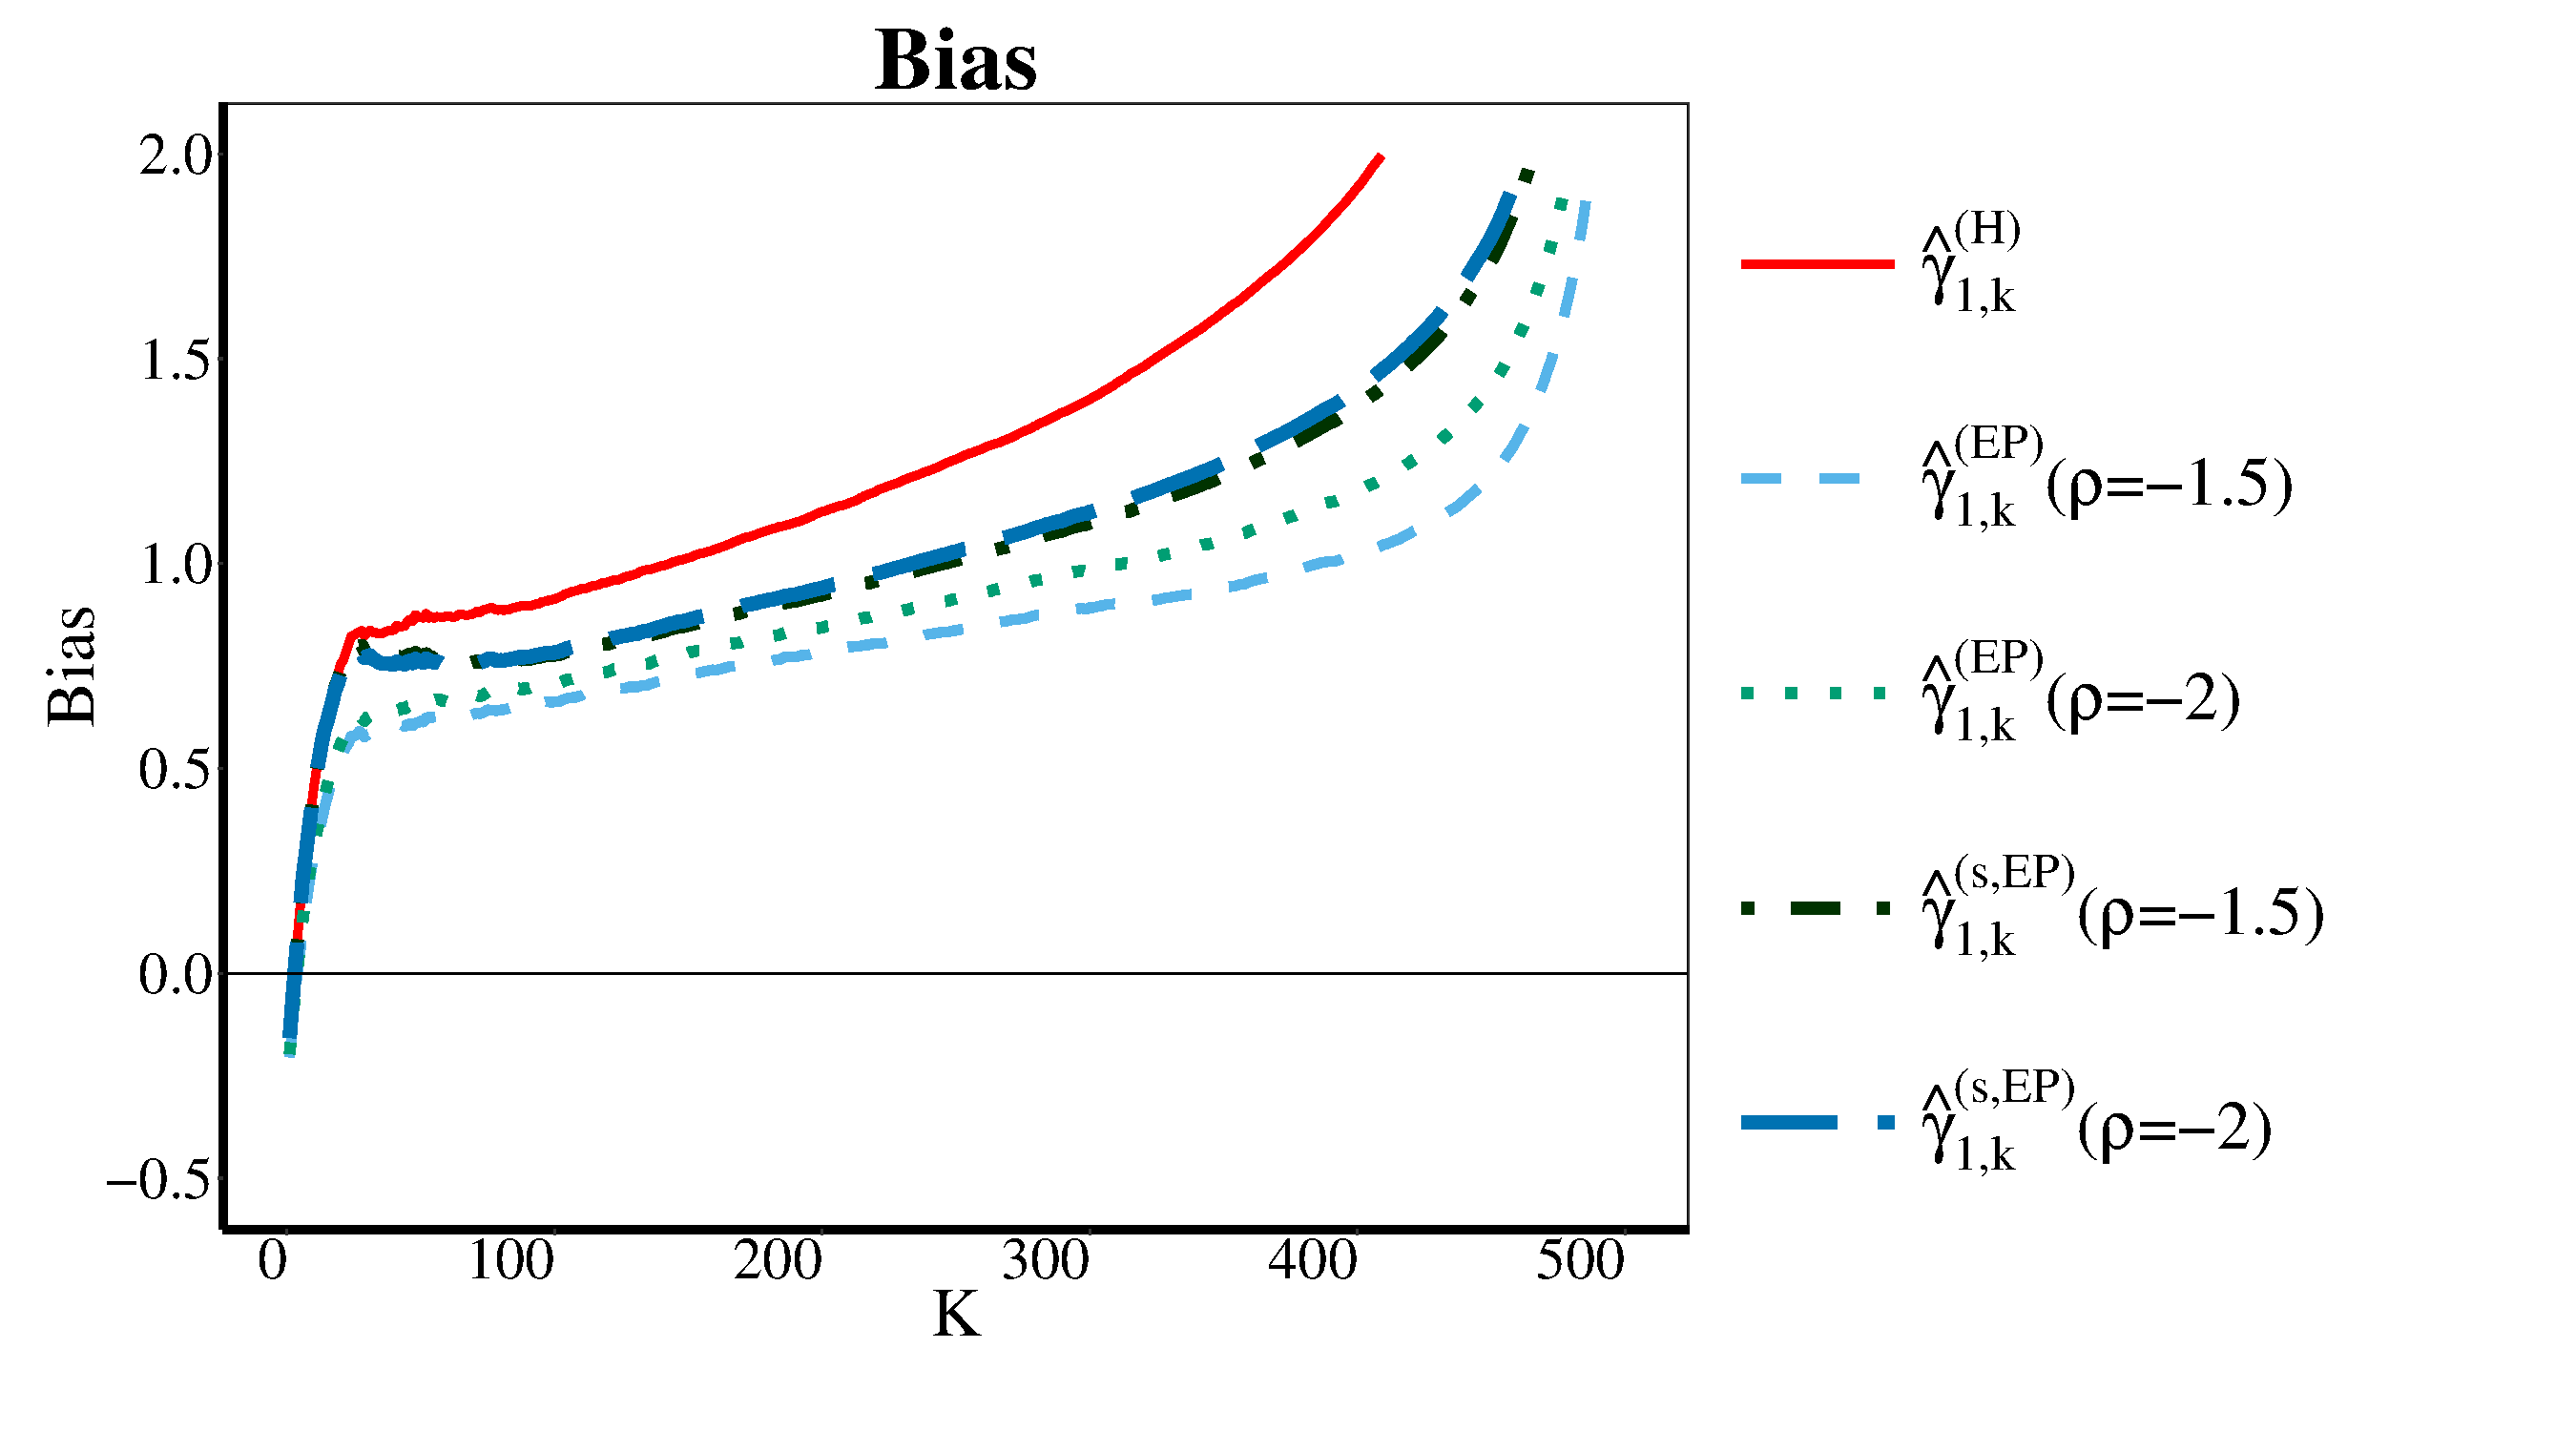
\includegraphics[width=7.5cm,height=5.5cm]{./plots/paper2/Bias_simulations_B12_H.pdf}
	\end{subfigure}
	\hspace{\fill}
	\begin{subfigure}[h]{0.3\linewidth}
		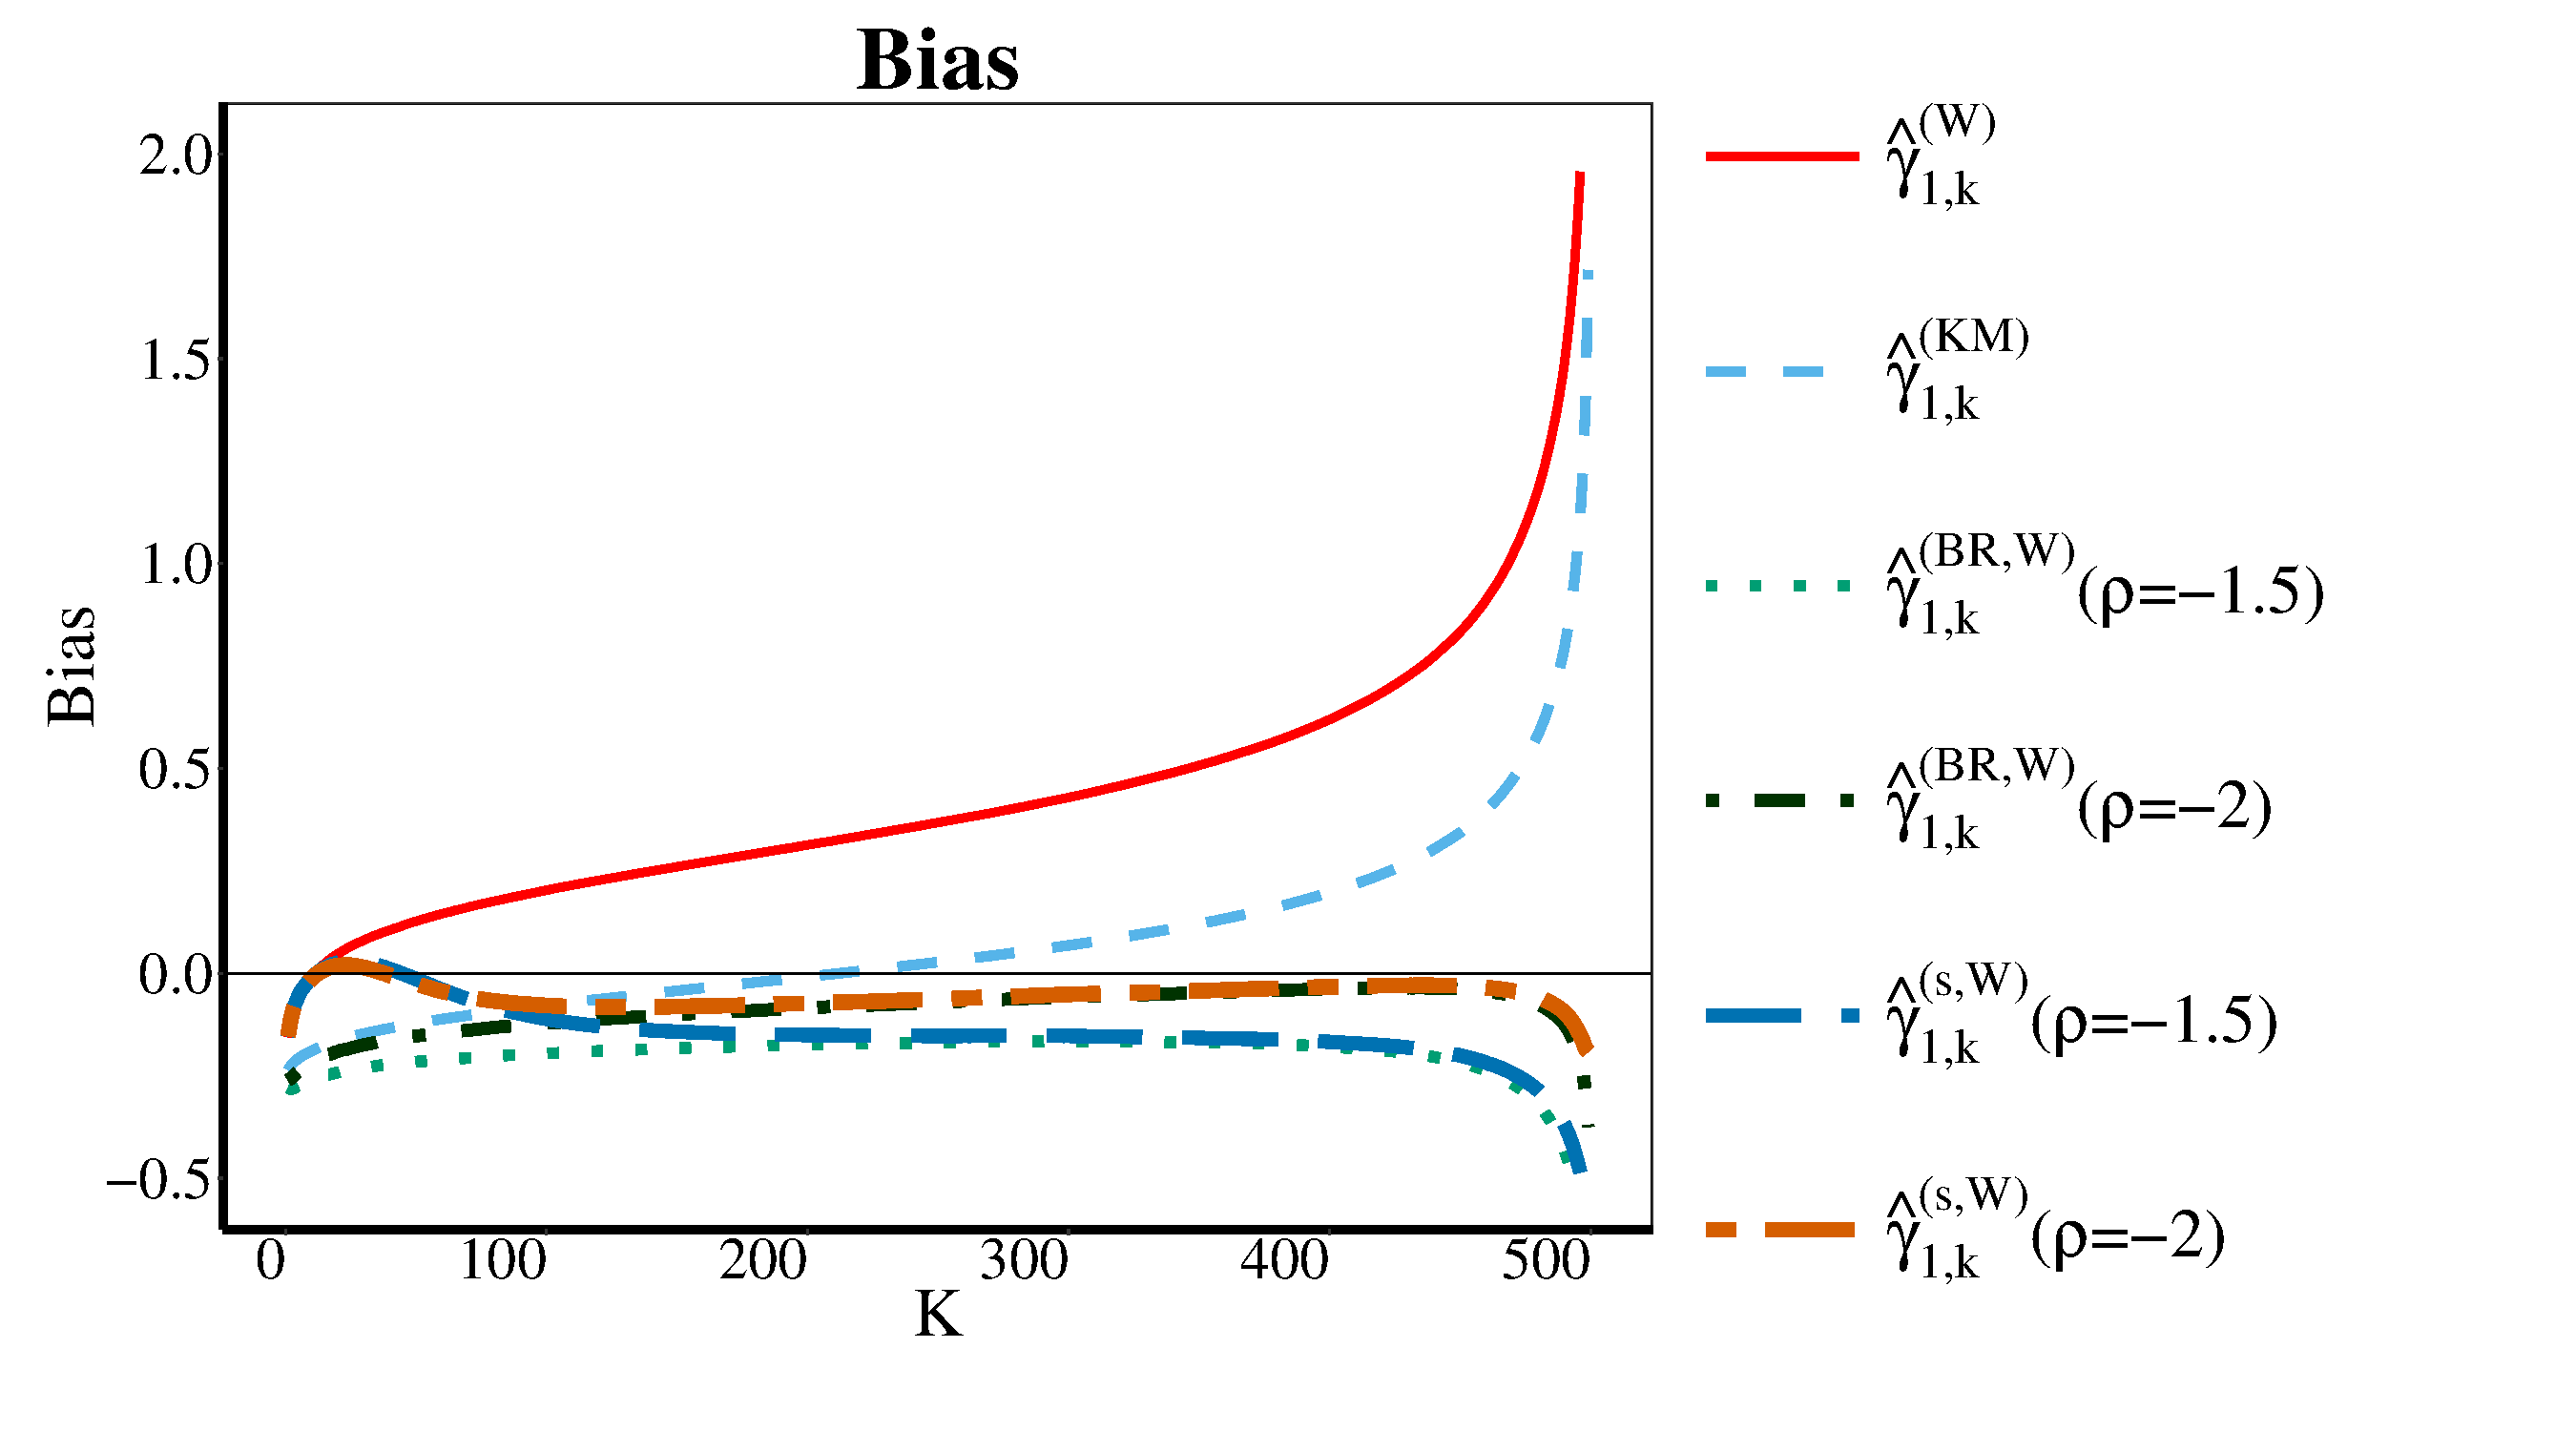
\includegraphics[width=7.5cm,height=5.5cm]{./plots/paper2/Bias_simulations_B12_W.pdf}
	\end{subfigure}
	\hspace{\fill}
	\begin{subfigure}[h]{0.3\linewidth}
		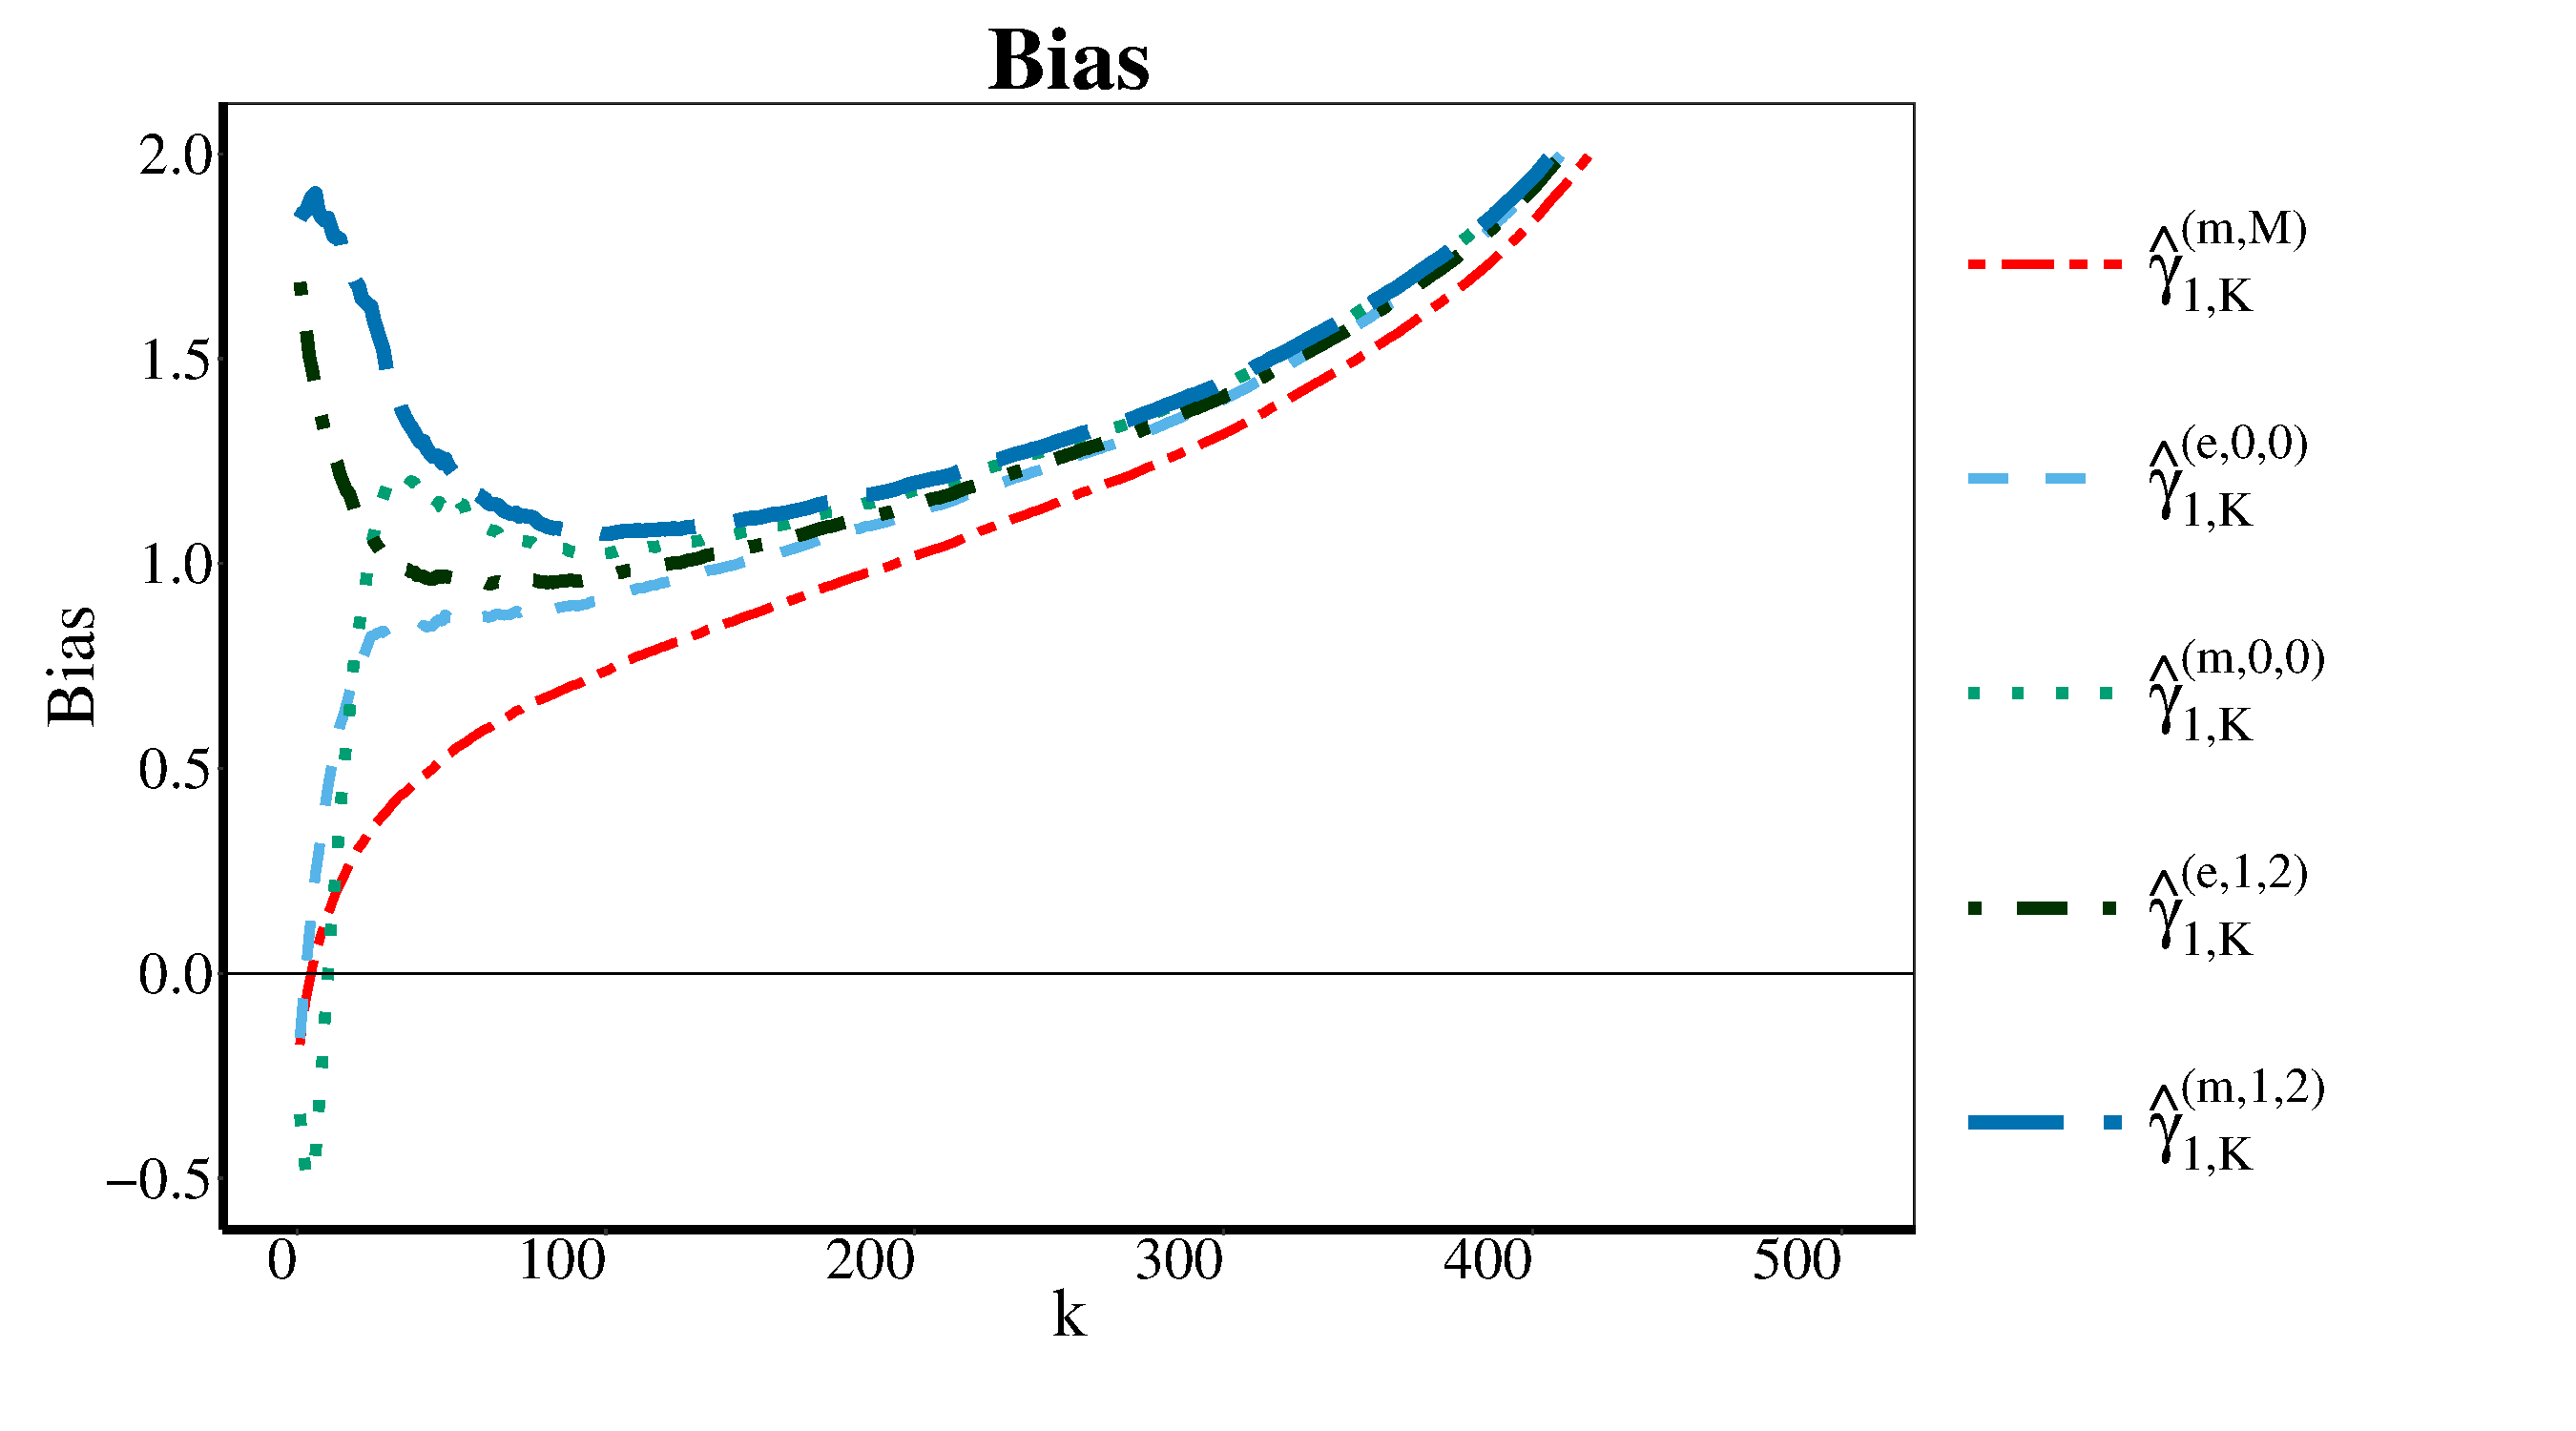
\includegraphics[width=6.5cm,height=5.5cm]{./plots/paper2/Bias_simulations_B12_B.pdf}
	\end{subfigure}
	\hspace{\fill}
	\begin{subfigure}[h]{0.3\linewidth}
		\includegraphics[width=7.5cm,height=5.5cm]{./plots/paper2/RMSE_simulations_B12_H.pdf}
	\end{subfigure}
		\hspace{\fill}
		\begin{subfigure}[h]{0.3\linewidth}
			\includegraphics[width=7.5cm,height=5.5cm]{./plots/paper2/RMSE_simulations_B12_W.pdf}
		\end{subfigure}
		\hspace{\fill}
		\begin{subfigure}[h]{0.3\linewidth}
			\includegraphics[width=6.5cm,height=5.5cm]{./plots/paper2/RMSE_simulations_B12_B.pdf}
		\end{subfigure}
		\caption{Bias and RMSE for \textbf{Burr(10,2,2)} censored by \textbf{Burr(10,5,2)}}
\label{paper2:fig1}
\end{figure}

%Figure2
\begin{figure}[h]
	\centering
	\begin{subfigure}[h]{0.3\linewidth}
		\includegraphics[width=7.5cm,height=5.5cm]{./plots/paper2/Bias_simulations_B11_H.pdf}
	\end{subfigure}
	\hspace{\fill}
	\begin{subfigure}[h]{0.3\linewidth}
		\includegraphics[width=7.5cm,height=5.5cm]{./plots/paper2/Bias_simulations_B11_W.pdf}
	\end{subfigure}
	\hspace{\fill}
	\begin{subfigure}[h]{0.3\linewidth}
		\includegraphics[width=6.5cm,height=5.5cm]{./plots/paper2/Bias_simulations_B11_B.pdf}
	\end{subfigure}
	\hspace{\fill}
	\begin{subfigure}[h]{0.3\linewidth}
		\includegraphics[width=7.5cm,height=5.5cm]{./plots/paper2/RMSE_simulations_B11_H.pdf}
	\end{subfigure}
	\hspace{\fill}
	\begin{subfigure}[h]{0.3\linewidth}
		\includegraphics[width=7.5cm,height=5.5cm]{./plots/paper2/RMSE_simulations_B11_W.pdf}
	\end{subfigure}
	\hspace{\fill}
	\begin{subfigure}[h]{0.3\linewidth}
		\includegraphics[width=6.5cm,height=5.5cm]{./plots/paper2/RMSE_simulations_B11_B.pdf}
	\end{subfigure}
	\caption{Bias and RMSE for \textbf{Burr(10,2,1)} censored by \textbf{Burr(10,2,1)}}
\label{paper2:fig2}
\end{figure}


%Figure3
\begin{figure}[h]
	\centering
	\begin{subfigure}[h]{0.3\linewidth}
		\includegraphics[width=7.5cm,height=5.5cm]{./plots/paper2/Bias_simulations_B21_H.pdf}
	\end{subfigure}
	\hspace{\fill}
	\begin{subfigure}[h]{0.3\linewidth}
		\includegraphics[width=7.5cm,height=5.5cm]{./plots/paper2/Bias_simulations_B21_W.pdf}
	\end{subfigure}
	\hspace{\fill}
	\begin{subfigure}[h]{0.3\linewidth}
		\includegraphics[width=6.5cm,height=5.5cm]{./plots/paper2/Bias_simulations_B21_B.pdf}
	\end{subfigure}
	\hspace{\fill}
	\begin{subfigure}[h]{0.3\linewidth}
		\includegraphics[width=7.5cm,height=5.5cm]{./plots/paper2/RMSE_simulations_B21_H.pdf}
	\end{subfigure}
	\hspace{\fill}
	\begin{subfigure}[h]{0.3\linewidth}
		\includegraphics[width=7.5cm,height=5.5cm]{./plots/paper2/RMSE_simulations_B21_W.pdf}
	\end{subfigure}
	\hspace{\fill}
	\begin{subfigure}[h]{0.3\linewidth}
		\includegraphics[width=6.5cm,height=5.5cm]{./plots/paper2/RMSE_simulations_B21_B.pdf}
	\end{subfigure}
	\caption{Bias and RMSE for \textbf{Burr(10,5,2)} censored by \textbf{Burr(10,2,2)}}
\label{paper2:fig3}
\end{figure}




%Figure4

\begin{figure}[h]
	\centering
	\begin{subfigure}[h]{0.3\linewidth}
		\includegraphics[width=7.5cm,height=5.5cm]{./plots/paper2/Bias_simulations_F21_H.pdf}
	\end{subfigure}
	\hspace{\fill}
	\begin{subfigure}[h]{0.3\linewidth}
		\includegraphics[width=7.5cm,height=5.5cm]{./plots/paper2/Bias_simulations_F21_W.pdf}
	\end{subfigure}
	\hspace{\fill}
	\begin{subfigure}[h]{0.3\linewidth}
		\includegraphics[width=6.5cm,height=5.5cm]{./plots/paper2/Bias_simulations_F21_B.pdf}
	\end{subfigure}
	\hspace{\fill}
	\begin{subfigure}[h]{0.3\linewidth}
		\includegraphics[width=7.5cm,height=5.5cm]{./plots/paper2/RMSE_simulations_F21_H.pdf}
	\end{subfigure}
	\hspace{\fill}
	\begin{subfigure}[h]{0.3\linewidth}
		\includegraphics[width=7.5cm,height=5.5cm]{./plots/paper2/RMSE_simulations_F21_W.pdf}
	\end{subfigure}
	\hspace{\fill}
	\begin{subfigure}[h]{0.3\linewidth}
		\includegraphics[width=6.5cm,height=5.5cm]{./plots/paper2/RMSE_simulations_F21_B.pdf}
	\end{subfigure}
	\caption{Bias and RMSE for \textbf{Fr\'echet(2)} censored by \textbf{Fr\'echet(1)}}
\label{paper2:fig4}
\end{figure}

%Figure5


\begin{figure}[h]
	\centering
	\begin{subfigure}[h]{0.3\linewidth}
		\includegraphics[width=6.5cm,height=5.5cm]{./plots/paper2/zoomBias_simulations_B12_W.pdf}
	\end{subfigure}
	\hspace{\fill}
	\begin{subfigure}[h]{0.3\linewidth}
		\includegraphics[width=6.5cm,height=5.5cm]{./plots/paper2/zoomBias_simulations_B11_W.pdf}
	\end{subfigure}
	\hspace{\fill}
	\begin{subfigure}[h]{0.3\linewidth}
		\includegraphics[width=6.5cm,height=5.5cm]{./plots/paper2/zoomBias_simulations_B21_W.pdf}
	\end{subfigure}
	\hspace{\fill}
	\begin{subfigure}[h]{0.3\linewidth}
		\includegraphics[width=6.5cm,height=5.5cm]{./plots/paper2/zoomRMSE_simulations_B12_W.pdf}
	\end{subfigure}
	\hspace{\fill}
	\begin{subfigure}[h]{0.3\linewidth}
		\includegraphics[width=6.5cm,height=5.5cm]{./plots/paper2/zoomRMSE_simulations_B11_W.pdf}
	\end{subfigure}
	\hspace{\fill}
	\begin{subfigure}[h]{0.3\linewidth}
		\includegraphics[width=6.5cm,height=5.5cm]{./plots/paper2/zoomRMSE_simulations_B21_W.pdf}
	\end{subfigure}
	\caption{Bias (top) and RMSE (bottom) for $\hat{\gamma}_{1,k}^{(W)}$, $\hat{\gamma}_{1,k}^{(BR,W)}(-1.5)$, $\hat{\gamma}_{1,k}^{(BR,W)}(-2)$, $\hat{\gamma}_{1,k}^{(s,W)}(-1.5)$, $\hat{\gamma}_{1,k}^{(s,W)}(-2)$ in case of \textbf{Burr(10,2,2)} censored by \textbf{Burr(10,5,2)} (left); \textbf{Burr(10,2,1)} censored by \textbf{Burr(10,2,1)} (middle); and \textbf{Burr(10,5,2)} censored by \textbf{Burr(10,2,2)} (right) }
\label{paper2:fig5}
\end{figure}


\begin{figure}[h]
		\centering
		\includegraphics[width=0.6\textwidth]{./plots/paper2/s001SimulatedCI.pdf}
		\includegraphics[width=0.6\textwidth]{./plots/paper2/k25SimulatedCI.pdf}
		\caption{Simulated bootstrap 95\% confidence intervals with adaptive choice of $k_1$ and $k_2$ using $\epsilon = 0.01$ (4 left frames) and using $k_1=k_2=25=5\%n$ for every sample (4 right frames)}
\label{paper2:fig6}
			\end{figure}
\end{landscape}

\begin{figure}[h]
		\centering
		\includegraphics[width=0.8\textwidth]{./plots/paper2/pk_sliced.pdf}
		\caption{Car liability data: plot of $\hat{p}_k$ as a function of $k/n$ for all claims jointly (thick full line) and for claims that arrived in different time intervals.} 
	\label{paper2:fig7}
	\end{figure}

\begin{figure}[h]
		\centering
		\includegraphics[width=0.49\textwidth]{./plots/paper2/Worms_sliced.pdf}
	\includegraphics[width=0.49\textwidth]{./plots/paper2/WormsBR_sliced.pdf}
		\caption{Car liability data: $\hat{\gamma}_{1,k}^{(W)}$ (left) and $\hat{\gamma}_{1,k}^{(BR,W)}(-3)$ (right) based on indexed cumulative payments at end of 2010, as a function of $k/n$ for all claims together (thick full line) and for claims arriving in different time periods}
\label{paper2:fig8}
	\end{figure}
	
	\begin{figure}[h]
		\centering
		\includegraphics[width=0.49\textwidth]{./plots/paper2/EWorms_sliced.pdf}
	\includegraphics[width=0.49\textwidth]{./plots/paper2/EWormsBR_sliced.pdf}
		\caption{Car liability data: $\hat{\gamma}_{1,k}^{(W)}$ (left) and $\hat{\gamma}_{1,k}^{(BR,W)}(-3)$ (right) for all claims arriving in 1995-1999 and based on indexed cumulative payments at end of 2000(02)2010, as a function of $k/n$. }
	\label{paper2:fig9}
	\end{figure}
	
	\begin{figure}[h]
		\centering
			\includegraphics[width=0.49\textwidth]{./plots/paper2/k1k2WEVI12.pdf}
			\includegraphics[width=0.49\textwidth]{./plots/paper2/sWEVI73_50.pdf}
		\caption{Car liability data, using all claims: $\hat{\gamma}_{1,k}^{(W)}$, $\hat{\gamma}_{1,k}^{(s,W)}(-3)$, $\hat{\gamma}_{2,k}^{(W)}$, $\hat{\gamma}_{2,k}^{(s,W)}(-3)$ (left); 95\% bootstrap confidence intervals (right).}
	\label{paper2:fig10}
	\end{figure}
\part{Semi-parametric Refinements: General Tails ($\gamma\in \mathbb{R})$}\label{part2}
\chapter{Bias Reduced Peaks over Threshold Tail Estimation}\label{chap5}
\href{https://arxiv.org/abs/1810.01296}{\textit{This chapter is based on Beirlant, J., Maribe, G., Ph. Naveau and Verster, A., 2018. Bias Reduced Peaks over Threshold Tail Estimation, available on: arXiv:1810.01296}}
\setcounter{equation}{0} 
\section{Introduction} 
\label{Sec1}       % --- this section label
 Extreme value methodology starts from the assumption that the distribution of the available sample $X_1, X_2,\ldots,X_n$ belongs to the domain of attraction of a GEV distribution, i.e. there exists sequences $(b_n)_n$ and $(a_n>0)_n$ such that as $n \to \infty$
\begin{equation}
{\max (X_1, X_2,\ldots,X_n)-b_n \over a_n} \to _d Y_{\gamma},
\label{maxd}
\end{equation}
where $\mathbb{P} (Y_\gamma >y) = \exp (-(1+\gamma y)^{-1/\gamma})$, for some $\gamma \in \mathbb{R}$ with $1+\gamma y>0$. The parameter $\gamma$ is termed the EVI. It is well-known \citep[see e.g.][]{sts626,de2007extreme} that \eqref{maxd} is equivalent to the existence of a positive function $t \mapsto \sigma_t$, such that 
\begin{equation}
\mathbb{P}\left({X-t \over \sigma_t} >y| X>t \right)
= {\bar{F}(t+y\sigma_t) \over \bar{F}(t)} \to_{t \to x_+}
\bar{H}^{GP}_{\gamma}(y)= (1+\gamma y)^{-1/\gamma}, 
\label{POT}
\end{equation}
where $\bar{F}(x)=\mathbb{P}(X>x)$  and $x_+$ denotes the endpoint of the distribution of $X$. The conditional distribution of $X-t$ given $X>t$ is called the POT distribution, while $\bar{H}_{\gamma}^{GP}$ is the survival function of the GPD.\\
In case $\gamma >0$, the limit in \eqref{maxd} holds if and only if $F$ is of Pareto-type, i.e.
\begin{equation}
\bar{F}(x) = x^{-1/\gamma}\ell (x),
\label{Patype}
\end{equation} 
for some slowly varying function $\ell$, i.e. satisfying $\dfrac{\ell(yt)}{\ell (t)} \to 1 $ as $t \to \infty$, for every $y>1$. Pareto-type distributions satisfy a simpler POT limit result: as $t \to \infty$
\begin{equation}
\mathbb{P} \left( {X \over t} >y | X>t \right) \to \bar{H}^P_{\gamma}(y) := y^{-1/\gamma}, y>1. 
\label{POTPa}
\end{equation}

Estimation of $\gamma$ and tail quantities such as return periods is then based on fitting a GPD to the observed excesses $X-t$ given $X>t$, respectively a simple Pareto distribution with survival function $y^{-1/\gamma}$ to $X/t$ given $X>t$ in case $\gamma >0$.
The main difficulty in such an EV application is the choice of the threshold $t$. Most often, the threshold $t$ is chosen as one of the top data points $X_{n-k,n}$ for some $k \in \{1,2, \ldots,n \}$ where $X_{1,n} \leq X_{2,n} \leq \ldots \leq X_{n,n}$ denotes the ordered sample.
\\\\
The limit results in \eqref{POT} and \eqref{POTPa} require $t$ to be chosen as large as possible (or, equivalently, $k$ as small as possible) for the bias in the estimation of $\gamma$ and other tail parameters to be limited. However, in order to limit the estimation variance, $t$ should be as small as possible, i.e. the number of data points $k$ used in the estimation should be as large as possible. Several adaptive procedures for choosing $t$ or $k$ have been proposed, but mainly in the Pareto-type case with $\gamma >0$ under further second-order specifications of \eqref{Patype} or \eqref{POTPa}, see for instance \autoref{chap3} in \cite{sts626}, or \cite{matthys2000adaptive}.
\\\\
In case of a real-valued EVI, the selection of an appropriate threshold is even more difficult and only a few methods are available. \cite{beirlant2009second} proposed a penultimate limit distributions in \eqref{POT} and \eqref{POTPa}. In case $\gamma >0$, under the mathematical theory of second-order slow variation, i.e. assuming that 
\begin{equation}
\dfrac{\ell(yt)}{\ell (t)} - 1 =\delta_t 
\left( y^{-\beta}-1 \right),
\label{SO}
\end{equation}
where $\delta_t=\delta (t)= t^{-\beta}\tilde{\ell}(t)$, with $\beta >0$ and $\tilde\ell$ slowly varying at infinity (see section 2.3 in de Haan and Ferreira, 2006), the left hand side of \eqref{POTPa} equals
\[
\dfrac{\bar{F}(yt)}{\bar{F}(t)} = 
y^{-1/\gamma} \dfrac{\ell(yt)}{\ell (t)} =
y^{-1/\gamma} \left( 1 + \delta_t (y^{-\beta}-1)\right), \; y>1.
\]
This then leads to the extension of the Pareto distribution to approximate the distribution of $X/t$ given $X>t$ as $t \to \infty$:
\begin{equation}
\bar{H}_{\gamma,\delta}^{EP}(y) := y^{-1/\gamma}\left( 1+ \delta_t \left( (y^{-1/\gamma})^{\beta\gamma}-1\right)\right), \; y>1,
\label{EP}
\end{equation}
with $\delta_t$ satisfying $\delta_t \downarrow 0$ as $t \to \infty$.
 {\it In cases where the second order model \eqref{SO} holds}, such a mixture model $\bar{H}_{\gamma,\delta}^{EP}$ will improve the approximation of $\left( {X \over t} >u | X>t \right)$ for values of $t$ which are smaller than the appropriate $t$-values when modelling the POTs using $\bar{H}_{\gamma}^{P}$. So the extension can work when modelling large and moderate extremes. As a byproduct however, at instances, it may even work for the full sample.
\\
In \cite{beirlant2009second}, using an external estimator of $\rho=-\beta\gamma$, the parameters $(\gamma, \delta)$ are estimated fitting the EPD (slightly adapted, with survival function $ \left\{y (1+ \tilde{\delta}_t -\tilde{\delta}_t y^{-\beta}) \right\}^{-1/\gamma}$ and $\tilde\delta _t = \delta_t \gamma$) by maximum likelihood on excesses over a random threshold $X_{n-k,n}$, $k=1,2,\ldots,n$. 
The result of this procedure is two-fold:
\begin{itemize}
\item First, the estimates $\hat{\gamma}_k^{EP}$ of $\gamma$ are more stable as a function of $k$ compared to the original ML estimator derived by \cite{hill1975simple}
$$
H_{k,n} = {1 \over k} \sum_{j=1}^k \log {X_{n-j+1,n}\over X_{n-k,n}}
$$
 which is obtained by fitting the Pareto distribution $\bar{H}_{\gamma}^P$ to the excesses 
 $\{ {X_{n-j+1,n}\over X_{n-k,n}}, j=1,\ldots,k\}$ following \eqref{POTPa}. Indeed, the bias in the simple POT model \eqref{POTPa} is estimated when fitting $\bar{H}_{\gamma,\delta}^{EP}$ and it is shown that, under the assumption that the EP model for the excesses $X/t$ is correct and that $\beta$ is estimated consistently, the asymptotic bias of $\hat{\gamma}_k^{EP}$ is 0 as long as $k (k/n)^{2\beta\gamma} \to \lambda \geq 0$ as $k,n \to \infty$, while the asymptotic bias of $H_{k,n}$ is only 0 when $k (k/n)^{2\beta\gamma} \to 0$.
 \item On the other hand, the asymptotic variance of $\hat{\gamma}_k^{EP}$ equals $\left({1-\rho\over \rho}\right)^2 {\gamma^2 \over k}$, where ${\gamma^2 \over k}$ is the asymptotic variance of $H_{k,n}$. 
\end{itemize}
As an example Figure \ref{paper3:fig1} shows both the Hill estimates $H_{k,n}$ and the bias reduced estimates $\hat{\gamma}_k^{EP}$, obtained from maximum likelihood fitting of \eqref{EP} using $\rho=-\gamma\beta=-0.25, -0.5$ and $-1$, as a function of $k$ for a data set of Belgian ultimate car insurance claims from 1995 and 2010 discussed in more detail in \cite{albrecher2017reinsurance}. Note that the bias reduced estimates helps to interpret the original Hill ``horror" plot.
\\\\
Here from the bias reduced estimator a $\gamma$ level around 0.5 becomes apparent for $k \geq 200$ and a lower value between 0.3 and 0.4 for smaller values of $k$. In fact in insurance claim data mixtures in the ultimate tail do appear quite often. Moreover the EPD fit appears to extend quite well down to the lower threshold value, i.e. with $k$ up to 600 (but not when using almost all data, $k>600$).
In this sense, classical first order extreme value modelling can in some cases be extended using mixture modelling in order to capture the characteristics of the bulk of the data. 
\begin{figure}[!ht]
 \centering
\includegraphics[width=0.40\textwidth]{./plots/paper3/ultimates_xi.pdf} 
\caption{ Ultimates of Belgian car insurance claims: bias reduction of Hill estimator (full line) using $\bar{H}_{\gamma,\delta}^{EP}$ with $\rho=-0.25$ (dashed line), $\rho=-0.5$ (dotted line) and $\rho=-1$ (dash-dotted line).}
\label{paper3:fig1}
\end{figure}

In this section we concentrate on bias reduction when using the GPD approximation to the distribution of POTs $X-t|X>t$, on which the literature is quite limited. This allows to extend bias reduction to the general case $\gamma > -1/2$.  We apply the flexible semiparametric GP modelling introduced in \cite{tencaliec2018flexible} to the POT distributions. We also extend the second-order refined POT approach using $\bar{H}^{EP}_{\gamma,\delta}$ from \eqref{EP} to all max-domains of attraction.
Here the corresponding basic second order regular variation theory can be found in 
Theorem 2.3.8 in de Haan and Ferreira (2006) stating that
\begin{equation}
\lim_{t \to x_+}{ \mathbb{P}(X-t >y\sigma_t|X>t)- (1+\gamma y)^{-1/\gamma} \over \delta (t)} = (1+\gamma y)^{-1-1/\gamma}\Psi_{\gamma,\tilde{\rho}}((1+\gamma y)^{1/\gamma}),
\label{secondorder}
\end{equation}
with $\delta(t) \to 0$ as $t \to x_+$ and $\Psi_{\gamma,\tilde{\rho}}(x)={1 \over \tilde\rho}\left({x^{\gamma +\tilde{\rho}}-1 \over \gamma +\tilde\rho}- {x^{\gamma}-1 \over \gamma}\right)$ which for the cases $\gamma=0$ and $\tilde\rho=0$ is understood to be equal to the limit as $\gamma \to 0$ and $\tilde\rho \to 0$.
We further allow more flexible second-order models than the ones arising from second-order regular variation theory such as in \eqref{secondorder} using non-parametric modelling of the second-order component. These new methods are also applied to the specific case of Pareto-type distributions. 
\\

In the next section we propose our transformed and extended GPD models, and detail the estimation methods. Some basic asymptotic results are provided in \autoref{chap5:sec3}. In the final section we discuss simulation results of the proposed methods and some practical case studies. We then also discuss the evaluation of the overall goodness-of-fit behaviour of the fitted models.  

\section{Transformed and extended GPD models}

Recently, \cite{naveau2016modeling}, generalising \cite{papastathopoulos2013extended}, proposed to use full models for rainfall intensity data that are able to capture low, moderate and heavy rainfall intensities without a threshold selection procedure. These authors, considering only applications with a positive EVI however, propose to model all data jointly using transformation models with survival function 
\begin{equation}
\bar{F}(x) = 1-\bar{G}_0 \left( H^{GP}_{\gamma} ({x \over \sigma})\right)=: G_0\left( \bar{H}^{GP}_{\gamma} ({x \over \sigma})\right),
\label{naveau}
\end{equation}
with $\bar{G}_0$ and $G_0$ distribution functions on $[0,1]$ linked by $G_0(u)=1-\bar{G}_0 (1-u)$ ($0<u<1$), and satisfying constraints to preserve the classical tail GPD fit and a power behaviour for small rainfall intensities:
\begin{itemize}
\item $\lim_{u \downarrow 0} \dfrac{G_0(u)}{u}=a$, for some $a>0$,
%\item $\lim_{v \downarrow 0} \dfrac{G_0(v w(v))}{G_0(v)}=b$, for some $b>0$ where $v \mapsto w(v)$ is a positive function satsfying $w(v) = 1+ o(v)$ as $v \to 0$,
\item $\lim_{u \downarrow 0} \dfrac{\bar{G}_0(u)}{u^\kappa}=c$, for some $c>0$ and $\kappa >0$.
\end{itemize}
In \cite{naveau2016modeling} the authors propose parametric examples for $G_0$, such as 
$$G_0(u) = \dfrac{1+D}{D} u \left(1-\dfrac{u^D}{1+D}\right), v \in (0,1)\ \ \text{with}\ \ D>0.$$ 
In \cite{tencaliec2018flexible} a non-parametric approach is taken using Bernstein polynomials of degree $m$ to approximate $G_0$, i.e. using $G_{0}^{(m)} (u) = \sum_{j=0}^m G_0({j \over m})b_{j,m}(u)$ with beta densities
$$b_{j,m}(u)=\left( \begin{array}{c} m \\ j \end{array}\right)u^j (1-u)^{m-j},\; u \in (0,1).
$$ 
\\
In \cite{naveau2016modeling} and \cite{tencaliec2018flexible} the primary goal is the search for a model fitting the whole outcome set, while the fit of the proposed model to POT values $X-t |X>t$ for extrapolation purposes in order to estimate extreme quantiles and tail probabilities is imposed using the condition $\lim_{u \downarrow 0} \dfrac{G_0(u)}{u}=a$. However the bias and MSE properties of the estimators of $\gamma$ and $\sigma$ are still to be analyzed.\\

To encompass the above mentioned methods from \cite{beirlant2009second}, \cite{naveau2016modeling} and \cite{tencaliec2018flexible} we propose to approximate $\mathbb{P}\left(X-t >y| X>t \right)$ with a transformation model with right tail function of the type
\[\hspace{-3.5cm} ({\cal{T}}): \hspace{0.5cm}
\bar{F}^T_t (y) = G_t \left(\bar{H}^{GP}_{\gamma}({y \over \sigma})\right)
\]
where $G_t(u)/u \to 1$ for all $u \in (0,1)$ as $t \to x_+$. Note here that for $u \in (0,1)$ and \\ $Y=_d X-t|X>t$, 
\begin{equation}
G_t (u) = \mathbb{P} \left(\bar{H}^{GP}_{\gamma}({Y \over \sigma}) \leq u\right).
\label{Gt}
\end{equation} 

\noindent
We also consider a sub-model of $({\cal{T}})$, approximating the POT distribution with an extended GPD model
\[
({\cal{E}}) : \hspace{0.5cm} \bar{F}^E_t(y)= \bar{H}^{GP}_\gamma ({y \over \sigma})\left\{1 +\delta_t B_{\eta} \left( \bar{H}^{GP}_\gamma ( {y \over \sigma}) \right) \right\}, 
\]
where 
\begin{itemize}
\item $\delta_t =\delta (t) \to 0$ as $t \to x_+$,
%\item $\delta_t =\delta (t) \uparrow 1$ as $t \to 0$,
\item $B_{\eta} (1)=0$ and $\lim_{u \to 0} u^{1-\epsilon}B_{\eta}(u)=0$ for every $1>\epsilon >0$,
\item $B_{\eta}$ is twice continously differentiable. 
\end{itemize}
Here the parameter $\eta$ represents a second order (nuisance) parameter. 
For negative $\delta$-values one needs $\delta_t > \{\min_u (1-{d \over du}\, (uB_{\eta}(u))\}^{-1}$ to obtain a valid distribution. 
At $t=0$ the function $u \mapsto u(1+\delta_0 B_{\eta}(u))$ then corresponds to $u \mapsto G_0(u)$ in \eqref{naveau}, while ${G_t (u) \over u} \to 1$ as $t \to \infty$ leads to the GPD survival function $\bar{H}^{GP}_\gamma (x/\sigma)$ at large thresholds.
\\
Note that model ($\cal{E}$) is a direct generalisation of the EPD model \eqref{EP} replacing the Pareto distribution $y^{-1/\gamma}$ by the GPD $\bar{H}^{GP}_\gamma$ and considering a general function $B_\eta (u)$ rather than $ u^{\beta\gamma}-1 = u^{-\rho}-1$. 
\\
 
\noindent Now several possibilities for bias reduction appear:
\begin{enumerate}
\item[(1)] {\bf Estimation under the transformed model (${\cal T}$).} Modelling the distribution of $Y=X-t|X>t$
with model ($\cal{T}$) 
and estimating $G_t$ and $(\gamma,\sigma)$ for every $t$, we propose to use the algorithm from \cite{tencaliec2018flexible} for every $t$ or $k=1,\ldots,n$. This approach is further denoted with ($T\bar{p}$). \\
 Here we apply Bernstein approximation and estimation of $G_t$ which is the distribution function of $\bar{H}_{\gamma}^{GP}(Y/\sigma)$. 
The Bernstein approximation of order $m$ of a continuous distribution function $G$ on $[0,1]$
is given by 
\[
G^{(m)}(u) = \sum_{j=0}^m G\left( {j \over m}\right)\left( \begin{array}{c} m \\ j \end{array}\right)u^j (1-u)^{m-j},
\; u \in [0,1].
\]
As in Babu et al. (2002) one then replaces the unknown distribution function $G$ itself with the empirical distribution function $\hat{G}_n$ of the available data in order to obtain a smooth estimator of $G$:
\[
\hat{G}_n^{(m)}(u) = \sum_{j=0}^m \hat{G}_n\left( {j \over m}\right)\left( \begin{array}{c} m \\ j \end{array}\right)u^j (1-u)^{m-j}. 
\] 
In the present application, data from $G_t$ are only available after imputing a value for $(\gamma,\sigma)$. This then leads to the iterative algorithm from \cite{tencaliec2018flexible}, which is applied to every threshold $t$, or every number of top $k$ data. We here detail the algorithm for excesses $Y_{j,k}=X_{n-j+1,n}-X_{n-k,n}$ $(j=1,\ldots,k)$, using the reparametrization $(\gamma,\tau)$ with $\tau=\gamma/\sigma$:

\vspace{0.3cm}\noindent
{\it Algorithm} ($A_{\cal T}$) 
\begin{enumerate}
\item[(i)] Set starting values ($\hat{\gamma}_k^{(0)},\hat{\tau}_k^{(0)}$). Here one can use ($\hat{\gamma}_k^{ML},\hat{\tau}_k^{ML}$) from using $G_t (u)=u$.
\item[(ii)]
Iterate for $r=0,1,\ldots$ until the difference in loglikelihood taken in ($\hat{\gamma}_k^{(r)},\hat{\tau}_k^{(r)}$) and ($\hat{\gamma}_k^{(r+1)},\hat{\tau}_k^{(r+1)}$) is smaller than a prescribed value
\begin{enumerate}
\item Given ($\hat{\gamma}_k^{(r)},\hat{\tau}_k^{(r)}$)
construct rv's 
$ \hat{Z}_{j,k}= \left( 1+ \hat{\tau}_k^{(r)}Y_{j,k}\right)^{-1/\hat{\gamma}_k^{(r)}} 
$
\item Construct Bernstein approximation based on $\hat{Z}_{j,k}$ ($1\leq j \leq k$)
\[
\hat{G}_k^{(m)}(u) = \sum_{j=0}^m \hat{G}_k \left( {j \over m}\right)\left( \begin{array}{c} m \\ j \end{array}\right)u^j (1-u)^{m-j}
\]
with $\hat{G}_k$ the empirical distribution function of $\hat{Z}_{j,k}$
\item Obtain new estimates ($\hat{\gamma}_k^{(r+1)},\hat{\tau}_k^{(r+1)}$) with ML:
\begin{eqnarray*}
(\hat{\gamma}_k^{(r+1)},\hat{\tau}_k^{(r+1)})&=&
\mbox{argmax} \left\{
\sum_{j=1}^k \log \{ \hat{g}^{(m)}_k ((1+\tau \hat{Z}_{j,k})^{-1/\gamma})\} \right.\\
&& \hspace{1.5cm} \left. + \sum_{j=1}^k
\log \{{\tau \over \gamma}(1+\tau \hat{Z}_{j,k})^{-1-1/\gamma} \} \right\}
\end{eqnarray*}
with $\hat{g}^{(m)}_k $ denoting the derivative of $\hat{G}_k^{(m)}$.
\end{enumerate}
\end{enumerate}

\vspace{0.3cm}\noindent
The final estimates of $(\gamma,\tau)$ and $G_t$ are denoted here by $(\hat{\gamma}_k^T,\hat{\tau}_k^T)$ and $\hat{G}_k^T$. 
As noted in \cite{tencaliec2018flexible} the theoretical study of these estimates is difficult. In the simulation study the finite sample characteristics of these estimators $\hat{\gamma}_k^T$ are given using $m=k^a$ with a fixed value of $a$ using $\hat{a} = argmin \sum_{k=2}^n (\hat{\gamma}_k^T - \bar{\hat{\gamma}}^T_n)^2$ in order to stabilise the plots of the estimates of $\gamma$ as much as possible. Note that this estimation procedure is computationally demanding.

\vspace{0.2cm}\noindent
Estimates of small tail probabilities $\mathbb{P}(X>c)$ can be obtained through 
\[
\hat{\mathbb{P}}_k^T(X>c) = {k \over n} \hat{G}^T_k 
\left( \bar{H}_{\hat{\gamma}^T_k} ({\hat{\tau}^T_k \over \hat{\gamma}^T_k}(c-X_{n-k,n}) )\right).
\]
Finally, bias reduced estimators of extreme $1-p$ quantiles for small $p$ are obtained by setting the above formulas equal to $p$ and solving for $c$. 

\item[(2)] {\bf Estimation under the extended model (${\cal E}$).} Modelling the distribution of the exceedances $Y$ with model ($\cal{E}$) leads to maximum likelihood estimators based on the excesses $Y_{j,k}=X_{n-j+1,n}-X_{n-k,n}$ $(j=1,\ldots,k)$: 
\begin{eqnarray}
(\hat{\gamma}^E_k,\hat{\tau}^E_k, \hat{\delta}_k)&=&
\mbox{argmax} \left\{
\sum_{j=1}^k \log\left( 
1+\delta_k b_{\eta}((1+\tau Y_{j,k})^{-1/\gamma}) \right)
 \right. \nonumber \\
&& \hspace{1.5cm} \left. + \sum_{j=1}^k
\log \{{\tau \over \gamma}(1+\tau Y_{j,k})^{-1-1/\gamma} \}
%\textcolor{blue}{-\omega {\delta_k^2\over 2 \sigma_{k,n}^2} %
 \right\}
 \label{MLE}
\end{eqnarray}
with $b_{\eta}(u) ={d \over du} (uB_{\eta}(u))$ for a given choice of $B_\eta$.\\
\noindent
Estimates of small tail probabilities $\mathbb{P}(X>c)$ are then obtained through 
\[
\hat{\mathbb{P}}_k^E(X>c) = {k \over n} \bar{H}^{GP}_{\hat{\gamma}^E_k}\left({\hat{\tau}^E_k \over \hat{\gamma}^E_k}(c-X_{n-k,n}) \right) 
\left( 1+ \hat{\delta}_k^E \hat{B}_{\eta}\left(\bar{H}^{GP}_{\hat{\gamma}^E_k} ({\hat{\tau}^E_k \over \hat{\gamma}^E_k}(c-X_{n-k,n})\right)\right).
\]
 
\noindent
As in \cite{naveau2016modeling}, respectively \cite{tencaliec2018flexible}, two approaches can be taken towards the bias function $B_{\eta}$: a parametric approach, respectively a non-parametric approach. 
\begin{itemize}
\item[(a)] {\it In the parametric approach}, denoted ($Ep$), the second-order result \eqref{secondorder} leads to the parametric choice $B_{\gamma,\tilde{\rho}}(u)= {u^{\gamma} \over \tilde\rho}\left({u^{-\gamma -\tilde{\rho}}-1 \over \gamma +\tilde\rho}- {u^{-\gamma}-1 \over \gamma}\right)$ in case $\gamma+\tilde\rho \neq 0$ and $\gamma \neq 0$. \\\\
Model (${\cal{E}}$) allows for bias reduced estimation of $(\gamma,\tau)$ under the assumption that the corresponding second-order model \eqref{secondorder} is correct for the POTs $X-t|X>t$. Note that ($Ep$) generalises the approach taken in \cite{beirlant2009second} to all max-domains of attraction. When model (${\cal E}$) is used as a model for all observations, i.e. taking $t=0$, this model directly encompasses the models from \cite{frigessi2002dynamic} and \cite{naveau2016modeling}.\\
Here
\[b_\eta (u)= u^{-\tilde\rho}\left( {1-\tilde\rho\over \tilde\rho (\gamma +\tilde\rho)}\right)
+ u^\gamma \left( {1-\gamma \over \gamma (\gamma +\tilde\rho)}\right)
- {1 \over \gamma\tilde\rho},
\]
in which the classical estimator of $\gamma$ (with $\delta_k=0$), or an appropriate value $\gamma_0$, is used to substitute $\gamma$, next to an appropriate value of $\tilde\rho$. One can also choose a value of ($\gamma_0,\tilde\rho$) minimising the variance in the plot of the resulting estimates of $\gamma$ as a function of $k$.
 
\item[(b)] Alternatively, {\it a non-parametric approach} (denoted $E{\bar{p}}$) can be performed using the Bernstein polynomial algorithm from \cite{tencaliec2018flexible}. In fact in practice a particular distribution probably follows laws of nature, environment or business and does not have to follow the second-order regular variation assumptions as in \eqref{secondorder}. Moreover in the case of a real-valued EVI, the function $B_{\eta}$ can take different mathematical forms depending on ($\gamma,\tilde\rho$) and $\gamma+\tilde\rho$ being close to 0 or not.\\\\
Here a Bernstein type approximation is obtained for $u\mapsto uB_\eta (u)$ from
$\hat{G}_{k_*}^{(m)}(u) -u$ obtained through algorithm ($A_{\cal T}$), and reparametrizing $\delta_k$ by $\delta_k/\delta_{k_*}$ with $k_*$ an appropriate value of the number of top data used.
% We take $k_* \sim n^{1-\epsilon}$ for a small %value of $\epsilon$. 
The function $b_\eta (u)$ is then substituted by
$-1 + {d \over du}\hat{G}_{k_*}^{(m)}(u)$.
 \end{itemize}
 
\end{enumerate}
 
\vspace{0.5cm}\noindent
The methods described above of course can be rewritten for the specific case of Pareto-type distributions where the distribution of POTs $Y={X \over t}|X>t$ are approximated by transformed Pareto distributions. The models are then rephrased as 
 \[\hspace{-2.9cm} ({\cal{T}^+}): \hspace{0.5cm}
\bar{F}^E_t (y) = G_t \left(\bar{H}^{P}_{\gamma}(y)\right),
\]
where for $u \in (0,1)$ 
\begin{equation*}
G_t (u) = \mathbb{P} \left(\bar{H}^{P}_{\gamma}(Y) \leq u\right),
%\label{Gt}
\end{equation*} 
and
\[
({\cal{E}^+}) : \hspace{0.5cm} \bar{F}^E_t(y)= \bar{H}^{P}_\gamma (y)\left\{1 +\delta_t B_{\eta} \left( \bar{H}^{P}_\gamma (y) \right) \right\}. 
\]
The above algorithms, now based on the exceedances $Y_{j,k}= X_{n-j+1,n}/X_{n-k,n}$ ($j=1,\ldots,k$), are then adapted as follows:\\
$\bullet$ In algorithm ($A_{\cal T}$) step (ii.c) is replaced by 
\[
\hat{\gamma}_k^{(r+1)}=
\mbox{argmax} \left\{
\sum_{j=1}^k \log \{ \hat{g}^{(m)}_k ( (\hat{Z}_{j,k})^{-1/\gamma})\} + \sum_{j=1}^k
\log \{{1 \over \gamma}(\hat{Z}_{j,k})^{-1-1/\gamma} \} \right\},
\]
with $ \hat{Z}_{j,k}= Y_{j,k}^{-1/\hat{\gamma}_k^{(r)}} $. 
The resulting estimates are denoted with $\hat{\gamma}^{T+}_{k}$ and $\hat{G}^{T+}_k $.
 \\
$\bullet$ In approach (${\cal E}$) the likelihood solutions are given by
\begin{equation}
(\hat{\gamma}^{E+}_k, \hat{\delta}^{E+}_k)=
\mbox{argmax} \left\{
\sum_{j=1}^k \log\left( 
1+\delta_k b_{\eta}(Y_{j,k}^{-1/\gamma}) \right)+
 \sum_{j=1}^k
\log \{{1 \over \gamma} (Y_{j,k})^{-1-1/\gamma} \}
 \right\}.
\label{E+}
\end{equation}
Note that the ($Ep^+$) approach using the parametric version $B_\eta (u) = u^{-\rho}-1$ for a particular fixed $\rho <0$ equals the EPD method from \cite{beirlant2009second}, while ($E\bar{p}^+$) is new.

\vspace{0.2cm}\noindent
Estimators of tail probabilities are then given by 
\[
\hat{\mathbb{P}}_k^{T+}(X>c) = {k \over n} \hat{G}^{T+}_k 
\left( \bar{H}_{\hat{\theta}^{T+}_k} \; (c/X_{n-k,n})\right),
\]
respectively
\[
\hat{\mathbb{P}}_k^{E+}(X>c) = {k \over n} \bar{H}^{P}_{\hat{\gamma}^{E+}_k}\left( c/X_{n-k,n} \right) 
\left( 1+ \hat{\delta}_k^{E+} \hat{B}_{\eta}\left(\bar{H}^{P}_{\hat{\gamma}^{E+}_k} (c/X_{n-k,n})\right)\right).
\]
 

\section{Basic asymptotics under model (${\cal E}$)}\label{chap5:sec3}

We discuss here in detail the asymptotic properties of the maximum likelihood estimators solving \eqref{MLE} and \eqref{E+}. To this end, as in \cite{beirlant2009second} we develop the likelihood equations up to linear terms in $\delta_k$ since $ \delta_k \to 0$ with decreasing value of $k$. 
Below we set $\bar{H}_{\theta}(y)=(1+\tau y)^{-1/\gamma}$ when using extended GPD modelling, while $\bar{H}_{\theta}(y)=y^{-1/\gamma}$ when using EP modelling under $\gamma >0$.

\vspace{0.2cm}\noindent
{\it Extended Pareto POT modelling}. The likelihood problem \eqref{E+} was already considered in \cite{beirlant2009second} in case of parametric modelling for $B_\eta$. We here propose a more general treatment. The limit statements in the derivation can be obtained using the methods from \cite{beirlant2009second}. The likelihood equations following from \eqref{E+} are given by
\begin{equation}
\left\{
\begin{array}{lcl}
{\partial \over \partial \gamma} \ell &=&
-{k \over \gamma }+ {1 \over \gamma^2} \sum_{j=1}^k \log Y_{j,k}
 + {\delta_k \over \gamma^2} \sum_{j=1}^k \dfrac{ b'_\eta (\bar{H}_{\theta}(Y_{j,k}))\bar{H}_{\theta}(Y_{j,k})\log Y_{j,k}}{1+\delta_k b_\eta (\bar{H}_{\theta}(Y_{j,k}))} \\
 {\partial \over \partial \delta_k} \ell &=&
 \sum_{j=1}^k b_\eta (\bar{H}_{\theta}(Y_{j,k}))-\delta_k \sum_{j=1}^k b^2_\eta (\bar{H}_{\theta}(Y_{j,k})).
\end{array}
\right.
\label{systemE+}
\end{equation}

\vspace{0.2cm}\noindent
{\it Extended Generalised Pareto POT modelling}. 
The likelihood equations following from \eqref{MLE} up to linear terms in $\delta_k$ are now given by
\[
\left\{
\begin{array}{lcl}
{\partial \over \partial \gamma} \ell &=&
-{k \over \gamma }+ {1 \over \gamma^2} \sum_{j=1}^k \log (1+\tau Y_{j,k})
 + {\delta_k \over \gamma^2} \sum_{j=1}^k b'_\eta (\bar{H}_{\theta}(Y_{j,k}))\bar{H}_{\theta}(Y_{j,k})\log (1+\tau Y_{j,k}) \\
 {\partial \over \partial \tau} \ell &=&
{k \over \gamma \tau}
\left\{ -1+ (1+\gamma) {1 \over k}\sum_{j=1}^k {1 \over 1+\tau Y_{j,k}} \right. \\
&& \hspace{1cm} \left. 
 -{\delta_k \over k}\sum_{j=1}^k b'_\eta (\bar{H}_{\theta}(Y_{j,k})) (\tau Y_{j,k}) (1+\tau Y_{j,k})^{-1-1/\gamma}
  \right\}
 \\
 {\partial \over \partial \delta_k} \ell &=&
 \sum_{j=1}^k b_\eta (\bar{H}_{\theta}(Y_{j,k}))-\delta_k \sum_{j=1}^k b^2_\eta (\bar{H}_{\theta}(Y_{j,k})),
\end{array}
\right.
\]
from which
\begin{equation}
 \left\{
\begin{array}{l}
\hat{\delta}_k = \dfrac{\sum_{j=1}^k b_\eta (\bar{H}_{\hat{\theta}_k}(Y_{j,k}))}{\sum_{j=1}^k b^2_\eta (\bar{H}_{\hat{\theta}_k}(Y_{j,k}))}, \\
{1 \over k}\sum_{j=1}^k \log (1+\hat{\tau}_k Y_{j,k})
= \hat{\gamma}_k- 
{\hat{\delta}_k \over k}\sum_{j=1}^k b'_{\eta}(\bar{H}_{\hat{\theta}_k}(Y_{j,k})) \bar{H}_{\hat{\theta}_k}(Y_{j,k}) \log (1+\hat{\tau}_k Y_{j,k}), \\
{1 \over k}\sum_{j=1}^k {1 \over 1+\hat{\tau}_k Y_{j,k}}
= {1 \over 1+ \hat{\gamma}_k} 
+ {\hat{\delta}_k \over 1+ \hat{\gamma}_k}
\left\{ 
{1\over k}\sum_{j=1}^k b'_{\eta}(\bar{H}_{\hat{\theta}_k}(Y_{j,k}))\bar{H}_{\hat{\theta}_k}(Y_{j,k}) \right.\\
 \hspace{6cm} \left.
- {1\over k}\sum_{j=1}^k b'_{\eta}(\bar{H}_{\hat{\theta}_k}(Y_{j,k}))\bar{H}_{\hat{\theta}_k}(Y_{j,k}) {1 \over 1+\hat{\tau}_k Y_{j,k}}
 \right\}.
\end{array}
\right.
\label{systemE}
\end{equation}

\vspace{0.3cm}\noindent
Under the extended model we now state the asymptotic distribution of the estimators $\hat{\gamma}_k^{E+}$ and $\hat{\gamma}_k^{E}$. To this end let $Q$ denote the quantile function of $F$, and let $U(x)=Q(1-x^{-1})$ denote the corresponding tail quantile function. 
Model assumption $({\cal{E}})$ can be rephrased in terms of $U$: 
\[
({\tilde{\cal{E}}}):\;\;
\dfrac{\dfrac{U(vx)-U(v)}{\sigma_{U(v)}} -h_{\gamma}(x)}{\delta (U(v))} \to _{v \to \infty} x^{\gamma} B_{\eta}(1/x),
\]
where $h_{\gamma}(x)= (x^{\gamma}-1)/\gamma$ and $\delta (U)$ regularly varying with index $\tilde\rho<0$. 
Moreover in the mathematical derivations one needs the extra condition that for every $\epsilon,\nu>0$, and $v, vx$ sufficiently large
\[
({\tilde{\cal{E}}}_2):\;\;
\left| \dfrac{\dfrac{U(vx)-U(v)}{\sigma_{U(v)}} -h_{\gamma}(x)}{\delta (U(v))} - x^{\gamma} B_{\eta}(1/x) \right| \leq \epsilon x^{\gamma}|B_{\eta}(1/x)| \max\{x^{\nu},x^{-\nu}\}.
\]
Similarly, $({\cal{E}}^+)$ is rewritten as
\[
({\tilde{\cal{E}}}^+):\;\;
\dfrac{\dfrac{U(vx)}{U(v)} - x^{\gamma}}{\gamma \delta(U(v)))} \to_{v \to \infty} x^{\gamma} B_{\eta}(1/x).
\]
The analogue of 
$({\tilde{\cal{E}}}_2)$ in this specific case is given by
\[
({\tilde{\cal{E}}}_2^+):\;\;
\left| \dfrac{\dfrac{U(vx)}{U(v)} - x^{\gamma}}{\gamma\delta(U(v))} -
x^{\gamma} B_{\eta}(1/x) \right|
 \leq \epsilon x^{\gamma}|B_{\eta}(1/x)| \max\{x^{\nu},x^{-\nu}\},
\]
with $\delta(U)$ regularly varying with index $\rho <0$.\\
Finally, in the expression of the asymptotic variances we use 
\[
Eb^2_{\eta} = \int_0^1 b^2_{\eta} (u)du, \;\;
EB_{\eta} = \int_0^1 B_{\eta} (u)du, \;\;
EC_{\eta} = \int_0^1 u^{\gamma}B_{\eta} (u)du.
\]
The proof of the next theorem is outlined in Appendix \ref{appen1}. It allows to construct confidence intervals for the estimators of $\gamma$ obtained under the extended models.\\
\begin{theorem}\label{theorem1} {\it Let $k=k_n$ be a sequence such that $k,n \to \infty$ and $k/n \to 0$ such that $\sqrt{k}\delta (U(n/k)) \to \lambda \in \mathbb{R}$. Moreover assume that in \eqref{MLE}
and \eqref{E+}, $B_{\eta}$ is substituted by a consistent estimator as $n\to \infty$. Then
\begin{enumerate}
\item[i.] when $\gamma>0$ with $({\tilde{\cal{E}}}_2^+)$ 
$$\sqrt{k}\left( \hat{\gamma}_k^{E+} -\gamma \right) \to^d \mathcal{N}\left(0,\gamma^2 \dfrac{Eb^2_{\eta}}{Eb^2_{\eta}-(EB_{\eta})^2}\right),$$
\item[ii.] when $\gamma > -1/2$ with $({\tilde{\cal{E}}}_2)$ 
$$\left( \sqrt{k}( \hat{\gamma}_k^{E} -\gamma), \sqrt{k} ({\hat{\tau}^{E}_k\over \tau}-1) \right)\to^d \mathcal{N}_2({\bf 0},\Sigma)$$
\[
\Sigma ={\gamma^2 \over D}
\left( 
\begin{array}{ll}
{1 \over (1+\gamma)^2(1+2\gamma)} - \dfrac{ (EC_{\eta})^2}{Eb^2_{\eta}} 
 & 
{1 \over \gamma(1+\gamma)^3 }-\dfrac{EB_{\eta}EC_{\eta}}{\gamma(1+\gamma)Eb^2_{\eta}}
\\
{1 \over \gamma(1+\gamma)^3 }-\dfrac{EB_{\eta}EC_{\eta}}{\gamma(1+\gamma)Eb^2_{\eta}}
&
{1 \over \gamma^2(1+\gamma)^2}\left(1- \dfrac{(EB_{\eta})^2}{Eb^2_{\eta}} \right)
\end{array}
\right)
\]
where
\[
D=\left( {1 \over (1+\gamma)^2(1+2\gamma)} - \dfrac{ (EC_{\eta})^2}{Eb^2_{\eta}} \right)\left(1- \dfrac{(EB_{\eta})^2}{Eb^2_{\eta}}\right)
- \left( {1 \over (1+\gamma)^2 }- \dfrac{EB_{\eta}EC_{\eta}}{Eb^2_{\eta}}\right)^2,
\]
\end{enumerate} 
} $\blacktriangle$
\end{theorem}
\vspace{0.3cm}\noindent
\begin{remark} The asymptotic variance of $\hat{\gamma}_k^{E+}$ is larger than the asymptotic variance $\gamma^2$ of the Hill estimator $H_{k,n}$. Indeed, 
\begin{eqnarray*}
(EB_\eta)^2 &=& \left( \int_0^1 \log (1/u) b_{\eta}(u) du \right)^2 \\
&=& \left( \int_0^1 (\log (1/u) -1) b_{\eta}(u) du \right)^2 \\
&\leq & \left( \int_0^1 (\log (1/u) -1)^2 du \right)
\left( \int_0^1 b^2_{\eta}(u) du \right)\\
&=& (Eb^2_\eta),
\end{eqnarray*}
where the above inequality follows using the Cauchy-Schwarz inequality. \\
Similarly, one can show that
\[
(EC_\eta)^2= \gamma^{-2} \left(\int_0^1 (u^\gamma -{1 \over 1+\gamma})b_\eta du \right)^2 \leq {1 \over (1+2\gamma)(1+\gamma)^2}
(Eb^2_\eta).
\]
The asymptotic variance of $\hat{\gamma}_k^{E}$ equals 
\[
{(1+\gamma)^2 \over k} \;
\dfrac{1- (1+\gamma)^2(1+2\gamma)(EC_\eta)^2/(Eb_\eta^2)}
{1- {(1+\gamma)^4(1+2\gamma)\over \gamma^2} (Eb_\eta^2)^{-1}
[(EC_\eta)^2 -2 {(EC_\eta)(EB_\eta)\over (1+\gamma)^2}+ {(EB_\eta)^2 \over (1+\gamma)^{2}(1+2\gamma)}]
}
\]
\end{remark}
which can be shown to be larger than the asymptotic variance $(1+\gamma)^2/k$ of the classical GPD maximum likelihood estimator. In the parametric case with $B_\eta (u) = {u^{\gamma} \over \tilde\rho}\left({u^{-\gamma -\tilde{\rho}}-1 \over \gamma +\tilde\rho}- {u^{-\gamma}-1 \over \gamma}\right)$, one obtains $EB_\eta = (1+\gamma)^{-1}(1-\tilde\rho)^{-1}$, $EC_\eta = (1+\gamma)^{-1}(1+2\gamma)^{-1}
(\gamma-\tilde\rho+1)^{-1}$ and $Eb^2_\eta = 2 (1+2\gamma)^{-1}(1-2\tilde\rho)^{-1}(\gamma-\tilde\rho+1)^{-1}$. It then follows that the asymptotic variance of $\hat{\gamma}_k^{E}$ equals $\dfrac{(1+\gamma)^2}{k} \left(\dfrac{1-\tilde\rho}{\tilde\rho}\right)^2$.\\
In case $\gamma >0$ with $B_\eta (u)= u^{-\rho}-1$, the asymptotic variance of $\hat{\gamma}_k^{E+}$ is given by ${\gamma^2 \over k} \left(\dfrac{1-\rho}{\rho}\right)^2$ as already found in \cite{beirlant2009second}.

\vspace{0.3cm}
Since in model (${\cal{E}}$) the $B_{\eta}$ factor is multiplied by $\delta_t$, the asymptotic distribution of tail estimators based on (${\cal{E}}$) will not depend on the asymptotic distribution of the estimator of $B_{\eta}$. As in \cite{beirlant2009second} when using the EPD model in the Pareto-type setting, one can rely in the parametric approach on consistent estimators of the nuisance parameter $\eta$ using a larger proportion $k_*$ of the data.
 Alternatively, one can also consider different values of $\eta$ in the parametric approach, and of $(k_*,m)$ in the non-parametric setting, and search for values of this nuisance parameter which stabilises the plots of the EVI estimates as a function of $k$ using the minimum variance principle for the estimates as a function of $k$. Clearly one loses the asymptotic unbiasedness in Theorem \ref{theorem1} if $B_{\eta}$ is not consistently estimated. However as becomes clear from the simulation results in many instances the EVI estimators are not very sensitive to such a misspecification, especially in the non-parametric approaches $T\bar{p}$, $T\bar{p}^+$, $E\bar{p}$
and $E\bar{p}^+$, and the proposed estimators can still outperform the classical maximum likelihood estimators based on the first order approximations of the POT distributions.  


\section{Simulations and case studies}
 
Simulation results and practical cases are proposed on
 
\url{https://phdshinygao.shinyapps.io/ExtendedModels/}
 
 \vspace{0.3cm}\noindent
Under {\it Simulations} one finds simulation results with sample sizes $n= 200$ for different distributions from each max-domain of attraction. The bias and MSE for the different estimators are plotted as a function of the number of exceedances $k$. 
Using the notation from the preceding sections one has a choice to apply the technique with $\bar{H}_{\theta}$ equal to the GPD, respectively the simple Pareto distribution (only when $\gamma>0$). \\

\noindent 
In case of the transformed models (${\cal T}$) one finds a slider to adapt the degree $m$ of the Bernstein polynoms along $m=k^a$ for different values of $a \in (0,1)$. One can also choose $a$ adaptively per sample so as to minimise the variance of $\hat{\gamma}_k$ over $k=2,\ldots,n$ (in order to have stable plots over $k$).
 \\
 
 \noindent
In case of the extended models (${\cal E}$) one finds sliders for the following parameters:
\begin{itemize}
\item in case of Pareto modelling: $\rho$ in $Ep^+$, and $(k_*,m)$ in $E{\bar p}^+$ estimation;
\item in case of GPD modelling: $\tilde\rho$ in $Ep$, and $(k_*,m)$ in $E{\bar p}$ estimation.
\end{itemize}
Again one can indicate to choose these parameters so as to minimise the variance of $\hat{\gamma}_k$ over $k=2,\ldots,n$. 
 The value of $\gamma$ in the parametric function $B_{\gamma,\tilde\rho}$ in $Ep$ is imputed with the classical GPD-ML estimator at the given value of $k$.
\\

\noindent 
Also bias and RMSE plots of the corresponding tail probability estimates of $p=\mathbb{P}(X>c)$ are given, where $c$ is chosen so that these probabilities equal $p=0.005$ or $p=0.003$. Here the bias, respectively RMSE, are expressed as the average, respectively the average of squared values, of $\log (p/\hat{p})$. 
 \\ 
 
One can also change the vertical scale of the plots, smooth the figures by taking moving averages of a certain number of estimates. Finally one can download the figures as a `\verb|.pdf|' file type. \\
 
 
\noindent 
 
 
While on the above link, several other distributions are used and sliders are provided for the different parameters $a$, $m$, $\rho$, $\tilde\rho$, and $k_*$, we collect here the resulting figures for estimation of $\gamma$ and estimating 0.003 tail probabilities, when using the minimum variance principle for all parameters, in case of the following subset of models: 
\begin{itemize}
\item
{\it The Burr$\left(\tau,\lambda\right)$ distribution} with $\bar{F}(x)= \left(1+x^{\tau} \right)^{-\lambda}$ for $x>0$ with $\tau=1$ and $\lambda=2$, so that $\gamma= {1 \over \tau\lambda}={1 \over 2}$ and $\rho= -{1 \over \lambda}= -{1 \over 2}$. 
\item
{\it The Fr\'echet$\,(2)$ distribution} with $\bar{F}(x)= 1-\exp \left(-x^{-2} \right)$ for $x>0$, so that $\gamma = \dfrac{1}{2}$ and $\rho= \tilde\rho=-1$.
%	\item 
% 	{\it The Log Gamma(4,2) distribution} with $\bar{F}(x)= {2^4 \over \gamma (4)}\int_x^\infty \, (\log u)^3 u^{-3}du$ for $x>1$, so that $\gamma = \dfrac{1}{2}$ and $\rho=0$.
\item 
{\it The standard normal distribution} with $\gamma=0$ and $\tilde{\rho}=0$.
\item 	{\it The Exponential distribution} with $\bar{F}(x) = e^{-\lambda x}$ for $x>0$, so that $\gamma=0$ and $\tilde{\rho}=0$.
%	\item 
%	{\it The Gamma(m,1) distribution} with density ${1 \over \gamma (m)}u^{m-1}e^{-u}$ for $u>0$, so that $\gamma=0$ and $\tilde{\rho}=0$.
%	\item 
%	{\it The Beta(0.5, 4) distribution} with $\bar{F}(x)= $ for $x\leq m$, so that $\gamma=-\dfrac{1}{4}$ in which case $\tilde{\rho}=-...$.
\item
{\it The Reversed Burr distribution} with 
$\bar{F}(x) =\left(1+(1-x)^{-\tau}\right)^{-\lambda}$
for $x< 1$ with $\tau=5$ and $\lambda=1$, so that $\gamma = -1/(\tau\lambda)=-\dfrac{1}{5}$ with $\tilde{\rho}=-1/\lambda=-1$.
 \item
{\it The extreme value Weibull distribution} with 
$F(x) =e^{-(1-x)^{\alpha}}$
for $x< 1$ with $\alpha =4$, so that $\gamma = -\dfrac{1}{4}$ with $\tilde{\rho}=-1$.
%	\item 
%	{\it The uniform (0,1) distribution} with $\gamma=-1$ and $\tilde{\rho}=-1$.
\end{itemize}


In general the minimum variance principle works well, though in some cases some improved results can be obtained by choosing specific values of the parameters $a$, $\rho$, $m$ and $k_*$. This is mainly the case for the Pareto-type models when using $T\bar{p}$ and $E\bar{p}$, such as for the Fr\'echet distribution. Also, in case of tail probability estimation using $Ep$ for cases with $\gamma <0$ particular choices of the corresponding parameters lead to improvements over the minimum variance principle.
\\
When using $GPD$ modelling of the exceedances, overall the $Ep$ approach yields the best results, both in estimation of $\gamma$ and tail probabilities. The improvement over the classical GPD maximum likelihood approach is smaller for $E\bar{p}$, and in case of situations where the second order parameter $\tilde\rho$ equals 0 then $E\bar{p}$ basically equals the ML estimators. 
\\\\
In case of simple Pareto modelling for $\gamma >0$ cases (see Figures \ref{paper3:fig3} and \ref{paper3:fig5}) the $Ep^+$ and $E\bar{p}^+$ approaches yield serious improvements over the Hill estimator, with small bias for $Ep^+$ and $E\bar{p}^+$, while parametric approach $Ep^+$ naturally exhibits the best RMSE. Note that when $\tilde\rho=0$ the conditions of the main theorem are not met, in which case the GPD and the bias reductions are known to exhibit a large bias. This is typically the case when $\gamma=0$. This is also known to be the case using simple Pareto modelling when $\rho=0$.\\
 
\noindent
Under {\it Applications} the app also offers the analysis of some case studies, some of which are discussed here in more detail. We use the ultimates of the Belgian ultimate car insurance claims used in Figure \ref{paper3:fig1}, in order to illustrate  $T\bar{p}^+$, $E\bar{p}^+$ and $Ep^+$, and the winter rainfall data at Mont-Aigoual station (1976-2015)  already used in \cite{tencaliec2018flexible} to illustrate $T\bar{p}$, $E\bar{p}$ and $Ep$. We then present estimates of $\gamma$, $\sigma$ and tail probabilities $\mathbb{P}(X>x_{n,n})$ with $x_{n,n}$ denoting the largest observation, so that the estimated probability is supposed to be close to $1/n$. An option is provided to construct confidence intervals for $\gamma$ on the basis of Theorem \ref{theorem1}. \\\\
In case $k=n$ the exceedances correspond to the reversely ordered data, i.e. $Y_{j,n}= X_{n-j+1,n}$. The goodness-of-fit for the {\it complete data set} can be analyzed choosing a specific value $\theta_0=(\gamma_0,\sigma_0)$ using the estimates of ($\gamma,\sigma$) which were obtained as a function of $k$, and by estimating the transformation $G$ using one (ii.b) step from the transformation algorithm ($A_{\mathcal T}$) with starting value ($\gamma_0,\sigma_0$) and with a chosen value $m=n^a$ with $a \in (0,1)$ (slider). We then construct transformed P-P plots
\begin{eqnarray}
 && \hspace{-1cm} \left( -\log (1-\hat{F}_n (X_{n-j+1,n})); -\log \hat{G}(\bar{H}_{\theta_0}(X_{n-j+1,n})) \right)
 \nonumber \\
 &=& 
\left( \log {n+1 \over j}; -\log \hat{G}_n^{(m)}(\bar{H}_{\theta_0}(X_{n-j+1,n})) \right), \; j=1,\ldots,n,
 \label{gof}
\end{eqnarray} 
 where $\hat{F}_n$ denotes the empirical distribution function based on $X_{n-j+1,n}$ ($j=1,\ldots,n$). The closer the plot lies to the diagonal, the better the fit of the model defined by the survival function $\hat{G}^{(m)} (\bar{H}_{\theta_0})$.\\
 
 \noindent
In Figure \ref{paper3:fig10}, the estimates of $\gamma$ and $\mathbb{P}(X>4 \, 564 \,759)$ using the minimum variance principle are given, next the goodness-of-fit plot as defined in \eqref{gof} with $\gamma_0=0.28$ and $m=n^{0.99}$. The estimates of $\gamma$ obtained from $Ep^+$ and $E\bar{p}^+$ are clearly most stable as a function of $k$ indicating the EVI value 0.4. The tail probability above the largest ultimate observation is also most stable for $Ep^+$ and $E\bar{p}^+$ indicating a value close to $1/n$ (indicated by the horizontal line). While the goodness-of-fit plot shows some deviations from the 45 degree line for the fitted transformation model, the presented overall global fit is useful (correlation equals 0.97). \\

 \noindent
In Figure \ref{paper3:fig11}, for the winter rainfall data the results for $E\bar{p}$ with $m=57$, $k_*=43$ indicate two levels for $\gamma$ (0.4 and ultimately at small $k$ close to 0), $\sigma$ (10 and 40 for small $k$) and tail probability $\mathbb{P}(X>162.05)$ (0.005 and 0.002 for small $k$, to be compared with $1/n=0.0018$), which indicates a change of statistical tail behaviour near the top. 
\\
Method $Ep$ with $\rho=-1$ yields almost the same result as the classical GPD-ML method, except for the tail probability where it is quite unstable. Finally the transformation approach $T\bar{p}$ yields very stable plots at compromise values 0.2 for $\gamma$, 10 for $\sigma$ and 0.003 for the tail probability. While the goodness-of-fit plot with $m=n^{0.99}$, $\sigma_0=10$ and $\gamma_0=0.21$ has a correlation 0.997, the transformation approach seems to be unable to catch the deviating tail component near the top data with an EVI value close to 0.

\section{Chapter conclusion} 

In this contribution we have constructed bias reduced estimators of tail parameters extending the classical POT method using the GPD. The bias can be modelled parametrically (for instance based on second order regular variation theory), or non-parametricallly using Bernstein polynomial approximations. A basic asymptotic limit theorem is provided for the estimators of the extreme value parameters which allows to compute asymptotic confidence intervals. A shinyapp has been constructed with which the characteristics and the effectiveness of the proposed methods are illustrated through simulations and practical case studies. From this it follows that within the proposed methods it is always possible to improve upon the classical POT method both in bias and RMSE. 
\newpage
\begin{figure}[!ht]
 \centering
\includegraphics[width=0.45\textwidth]{./plots/paper3/burr05GPD_evi.pdf} 
\includegraphics[width=0.45\textwidth]{./plots/paper3/burr05GPD_rmse.pdf} \\
\includegraphics[width=0.45\textwidth]{./plots/paper3/burr05GPD_tail.pdf}
\includegraphics[width=0.45\textwidth]{./plots/paper3/burr05GPD_tail_rmse.pdf} 
 \caption{ Burr distribution with $\gamma=0.5$ and $\rho=-0.5$. Estimation of $\gamma$ (top) and tail probability (bottom) using minimum variance principle, bias (left), RMSE (right): GPD-ML (full line), $T\bar{p}$ (dotted), $Ep$ (dash-dotted) and $E\bar{p}$ (dashed). }
\label{paper3:fig2}
\end{figure}
 \begin{figure}[!ht]
 \centering
 \includegraphics[width=0.45\textwidth]{./plots/paper3/burr05Pareto_evi.pdf} 
\includegraphics[width=0.45\textwidth]{./plots/paper3/burr05Pareto_rmse.pdf} \\
\includegraphics[width=0.45\textwidth]{./plots/paper3/burr05Pareto_tail.pdf}
\includegraphics[width=0.45\textwidth]{./plots/paper3/burr05Pareto_tail_rmse.pdf} 
\caption{Burr distribution with $\gamma=0.5$ and $\rho=-0.5$. Estimation of $\gamma$ (top) and tail probability (bottom) using minimum variance principle, bias (left), RMSE (right): Pareto-ML (full line), $T\bar{p}^+$ (dotted), $Ep^+$ (dash-dotted) and $E\bar{p}^+$ (dashed).}
 \label{paper3:fig3}
 \end{figure}
 
 \begin{figure}[!ht]
 \centering
\includegraphics[width=0.45\textwidth]{./plots/paper3/frechetGPD_evi.pdf} 
\includegraphics[width=0.45\textwidth]{./plots/paper3/frechetGPD_rmse.pdf} \\
\includegraphics[width=0.45\textwidth]{./plots/paper3/frechetGPD_tail.pdf}
\includegraphics[width=0.45\textwidth]{./plots/paper3/frechetGPD_tail_rmse.pdf} 
 \caption{ Fr\'echet distribution with $\gamma=0.5$. Estimation of $\gamma$ (top) and tail probability (bottom), bias (left), RMSE (right): GPD-ML (full line), $T\bar{p}$ (dotted, using minimum variance principle), $Ep$ with $\rho=-2$ (dash-dotted) and $E\bar{p}$ with $(k_*,m)=(190,150)$ (dashed). }
\label{paper3:fig4}
\end{figure}
 \begin{figure}[!ht]
 \centering
 \includegraphics[width=0.45\textwidth]{./plots/paper3/frechetPareto_evi.pdf} 
\includegraphics[width=0.45\textwidth]{./plots/paper3/frechetPareto_rmse.pdf} \\
\includegraphics[width=0.45\textwidth]{./plots/paper3/frechetPareto_tail.pdf}
\includegraphics[width=0.45\textwidth]{./plots/paper3/frechetPareto_tail_rmse.pdf} 
\caption{Fr\'echet distribution with $\gamma=0.5$. Estimation of $\gamma$ (top) and tail probability (bottom) using minimum variance principle, bias (left), RMSE (right): Pareto-ML (full line), $T\bar{p}^+$ (dotted), $Ep^+$ (dash-dotted) and $E\bar{p}^+$ (dashed).}
\label{paper3:fig5}
 \end{figure}
 \begin{figure}[!ht]
 \centering
\includegraphics[width=0.45\textwidth]{./plots/paper3/std_normalGPD_evi.pdf} 
\includegraphics[width=0.45\textwidth]{./plots/paper3/std_normalGPD_rmse.pdf} \\
\includegraphics[width=0.45\textwidth]{./plots/paper3/std_normalGPD_tail.pdf}
\includegraphics[width=0.45\textwidth]{./plots/paper3/std_normalGPD_tail_rmse.pdf} 
 \caption{ Standard normal distribution ($\gamma=0$ and $\tilde\rho=0$). Estimation of $\gamma$ (top) and tail probability (bottom) using minimum variance principle, bias (left), RMSE (right): GPD-ML (full line), $T\bar{p}$ (dotted), $Ep$ (dash-dotted) and $E\bar{p}$ (dashed).}
\label{paper3:fig6}
\end{figure}

 \begin{figure}[!ht]
 \centering
\includegraphics[width=0.45\textwidth]{./plots/paper3/gammaGPD_evi.pdf} 
\includegraphics[width=0.45\textwidth]{./plots/paper3/gammaGPD_rmse.pdf} \\
\includegraphics[width=0.45\textwidth]{./plots/paper3/gammaGPD_tail.pdf}
\includegraphics[width=0.45\textwidth]{./plots/paper3/gammaGPD_tail_rmse.pdf} 
 \caption{ The exponential distribution ($\gamma=0$ and $\tilde\rho=0$). Estimation of $\gamma$ (top) and tail probability (bottom) using minimum variance principle, bias (left), RMSE (right): GPD-ML (full line), $T\bar{p}$ (dotted), $Ep$ (dash-dotted) and $E\bar{p}$ (dashed).}
\label{paper3:fig7}
\end{figure}


 \begin{figure}[!ht]
 \centering
\includegraphics[width=0.45\textwidth]{./plots/paper3/model3GPD_evi.pdf} 
\includegraphics[width=0.45\textwidth]{./plots/paper3/model3GPD_rmse.pdf} \\
\includegraphics[width=0.45\textwidth]{./plots/paper3/model3GPD_tail.pdf}
\includegraphics[width=0.45\textwidth]{./plots/paper3/model3GPD_tail_rmse.pdf} 
 \caption{ Reversed Burr distribution ($\gamma=-0.2$ and $\tilde\rho=-1$). Estimation of $\gamma$ (top) and tail probability (bottom) using minimum variance principle, bias (left), RMSE (right): GPD-ML (full line), $T\bar{p}$ (dotted), $Ep$ (dash-dotted) and $E\bar{p}$ (dashed).}
\label{paper3:fig8}
\end{figure}

\begin{figure}[!ht]
 \centering
\includegraphics[width=0.45\textwidth]{./plots/paper3/weibullGPD_evi.pdf} 
\includegraphics[width=0.45\textwidth]{./plots/paper3/weibullGPD_rmse.pdf} \\
\includegraphics[width=0.45\textwidth]{./plots/paper3/weibullGPD_tail.pdf}
\includegraphics[width=0.45\textwidth]{./plots/paper3/weibullGPD_tail_rmse.pdf} 
 \caption{Extreme value Weibull distribution ($\gamma=-0.25$ and $\tilde\rho=-1$). Estimation of $\gamma$ (top) and tail probability (bottom) using minimum variance principle, bias (left), RMSE (right): GPD-ML (full line), $T\bar{p}$ (dotted), $Ep$ (dash-dotted) and $E\bar{p}$ (dashed).}
\label{paper3:fig9}
\end{figure}

\begin{figure}[!ht]
 \centering
\includegraphics[width=0.45\textwidth]{./plots/paper3/ultimates_evi.pdf} 
\includegraphics[width=0.45\textwidth]{./plots/paper3/ultimates_tail.pdf} \\
\includegraphics[width=0.45\textwidth]{./plots/paper3/ultimates_GoF.pdf}
 
 \caption{Ultimates of Belgian car insurance claims: estimation of $\gamma$ (top left), tail probability at maximum observation (top right): Pareto-ML (full line), $T\bar{p}^+$ (dotted), $Ep^+$ (dashed) and $E\bar{p}^+$ (dash-dotted). Goodness-of-fit plot (bottom).}
\label{paper3:fig10}
\end{figure} 

\begin{figure}[!ht]
 \centering
\includegraphics[width=0.45\textwidth]{./plots/paper3/winter_evi.pdf} 
\includegraphics[width=0.45\textwidth]{./plots/paper3/winter_sigma.pdf} \\
\includegraphics[width=0.45\textwidth]{./plots/paper3/winter_prob.pdf}
\includegraphics[width=0.45\textwidth]{./plots/paper3/winter_GoF.pdf}
 
 \caption{Winter rain data at Mont-Aigoual: estimation of $\gamma$ and $\sigma$ (top) and tail probability (bottom left) using minimum variance principle: GPD-ML (full line), $T\bar{p}$ (dotted), $Ep$ (dashed) and $E\bar{p}$ (dash-dotted). Goodness-of-fit plot (bottom right). }
\label{paper3:fig11}
\end{figure} 

\begin{subappendices}
\section{Proof of Theorem 5.1}\label{appen1}

In this section we provide details concerning the proof of Theorem \ref{theorem1}. 
\\
\noindent {\it Asymptotic distribution of 
$\hat{\gamma}_k^{E+}$}. \\
From \eqref{systemE+} we obtain up to linear terms in $\delta_k$ that (denoting $\hat{\gamma}_k$ for $\hat{\gamma}^{E+}_k$)
\[
\left\{
\begin{array}{lcl}
\hat{\delta}_k &=& \dfrac{\sum_{j=1}^k b_\eta (Y_{j,k}^{-1/\hat{\gamma}_k})}{\sum_{j=1}^k b^2_\eta (Y_{j,k}^{-1/\hat{\gamma}_k})} \\
\hat{\gamma}_k &=& H_{k,n} + \hat{\delta}_k B^{(1)}_{k},
\end{array}
\right.
\]
with $B^{(1)}_{k}= {1 \over k}\sum_{j=1}^k b'_\eta (Y_{j,k}^{-1/\hat{\gamma}_k})Y_{j,k}^{-1/\hat{\gamma}_k}\log Y_{j,k}$. As $k,n \to \infty$ and $k/n \to 0$ we have $B^{(1)}_{k} \to_p -\gamma \int_0^1 b'_{\eta}(u) u \log u du = -\gamma EB_\eta$.
% with $ EB_\eta = \int_0^1 B_\eta (u) du$. 
\\
Using a Taylor expansion on the numerator of the right hand side of the first equation leads to
\[
{1 \over k}\sum_{j=1}^k b_\eta (Y_{j,k}^{-1/\hat{\gamma}_k})
=
{1 \over k}\sum_{j=1}^k b_\eta (Y_{j,k}^{-1/\gamma})
- (\hat{\gamma}_k - \gamma) \gamma^{-1} (EB_\eta) \, (1+o_p(1)), 
\]
so that, with ${1 \over k}\sum_{j=1}^k b^2_\eta (Y_{j,k}^{-1/\hat{\gamma}_k}) \to_p E b^2_{\eta}$, up to lower order terms
\[
\hat{\delta}_k = {1 \over E b^2_{\eta}} {1 \over k}\sum_{j=1}^k b_\eta (Y_{j,k}^{-1/\gamma})
- (\hat{\gamma}_k - \gamma) \gamma^{-1}\dfrac{EB_\eta }{E b^2_{\eta}} \, (1+o_p(1)).
\]
Hence, inserting this expansion into $\hat{\gamma}_k = H_{k,n} + \hat{\delta}_k B^{(1)}_{k}$, 
finally leads to 
\begin{eqnarray*}
&&\sqrt{k}(\hat{\gamma}_k - \gamma)(1+o_p(1))\\&=&
\dfrac{E b^2_{\eta}}{E b^2_{\eta}-(EB_\eta)^2} \sqrt{k}\left(H_{k,n}-\gamma \right)
-
\dfrac{\gamma EB_\eta }{E b^2_{\eta}-(EB_\eta)^2 }\sqrt{k} \left( {1 \over k}\sum_{j=1}^k b_\eta (Y_{j,k}^{-1/\gamma})\right)\\
&=& \dfrac{E b^2_{\eta}}{E b^2_{\eta}-(EB_\eta)^2} \sqrt{k}\left(H_{k,n}-\gamma - \gamma \delta_k EB_\eta\right) 
\\ && \;\;
-
\dfrac{\gamma EB_\eta }{E b^2_{\eta}-(EB_\eta)^2 }\sqrt{k} \left( {1 \over k}\sum_{j=1}^k b_\eta (Y_{j,k}^{-1/\gamma})
- \delta_k E b^2_{\eta}
\right),
\end{eqnarray*}
with $\delta_k = \delta (U(n/k))$.
We now show that this final expression is a linear combination of two zero centered statistics (up to the required accuracy) which is asymptotically normal with the stated asymptotic variance. To this end let $Z_{n-k,n} \leq Z_{n-k+1,n} \leq \ldots \leq Z_{n,n}$ denote the top $k+1$ order statistics of a sample of size $n$ from the standard Pareto distribution with distribution function $z \mapsto z^{-1}$, $z>1$. Then from $({\tilde{\cal{E}}}_2^+) $
\begin{eqnarray*}
H_{k,n} &=& {1 \over k}\sum_{j=1}^k
\left(\log U(Z_{n-j+1,n})- \log U(Z_{n-k,n}) \right) \\
&=& {1 \over k}\sum_{j=1}^k \log \left\{
\left({Z_{n-j+1,n}\over Z_{n-k,n}}\right)^\gamma 
\left[
1+\gamma \delta (U(Z_{n-k,n}))B_\eta \left( {Z_{n-k,n} \over Z_{n-j+1,n}}\right) \right. \right. \\
&& \hspace{4.6cm}\left.\left.
+o_p(1)|\delta (U(Z_{n-k,n}))| |B_\eta \left( {Z_{n-k,n} \over Z_{n-j+1,n}}\right)| \left({Z_{n-j+1,n}\over Z_{n-k,n}}\right)^\epsilon 
\right]
\right\}\\
&=& \gamma {1 \over k}\sum_{j=1}^k \log {Z_{n-j+1,n}\over Z_{n-k,n}}
+ \gamma \delta (U(Z_{n-k,n}))B_\eta \left( {Z_{n-k,n} \over Z_{n-j+1,n}}\right)\\
&& \hspace{3.5cm}
+o_p(1)|\delta (U(Z_{n-k,n}))| |B_\eta \left( {Z_{n-k,n} \over Z_{n-j+1,n}}\right)| \left({Z_{n-j+1,n}\over Z_{n-k,n}}\right)^\epsilon. 
\end{eqnarray*}
Now $\log Z_{n-j+1,n}-\log Z_{n-k,n} =_d E_{k-j+1,k}$, the $(k-j+1)$th smallest value from a standard exponential sample $E_1,\ldots,E_k$ of size $k$, so that ${1 \over k}\sum_{j=1}^k \log {Z_{n-j+1,n}\over Z_{n-k,n}}=_d {1 \over k}\sum_{j=1}^k E_j$ and ${1 \over k}\sum_{j=1}^k B_\eta \left( {Z_{n-k,n} \over Z_{n-j+1,n}}\right) =_d {1 \over k}\sum_{j=1}^k B_\eta (e^{-E_j})=_d {1 \over k}\sum_{j=1}^k B_\eta (U_j)$ where $U_1,\ldots,U_k$ is a uniform (0,1) sample. Hence, since $\delta (U(Z_{n-k,n})) / \delta (U(n/k)) \to_p 1$ and ${1 \over k}\sum_{j=1}^k B_\eta (U_j) \to_p EB_{\eta}$, we have that $H_{k,n} -\gamma - \gamma \delta_k EB_\eta$ is asymptotically equivalent to $ {1 \over k}\sum_{j=1}^k \gamma (E_j-1)$ as $\sqrt{k} \delta_k \to \lambda$. \\
Similarly 
\begin{eqnarray*}
&&{1 \over k}\sum_{j=1}^k b_\eta (Y_{j,k}^{-1/\gamma})\\&=&
{1 \over k}\sum_{j=1}^k b_\eta \left(\left[ {U \left({Z_{n-j+1,n}\over Z_{n-k,n}} Z_{n-k,n} \right)\over U(Z_{n-k,n}) }\right]^{-1/\gamma} \right)\\
&=& {1 \over k}\sum_{j=1}^k b_\eta
\left(
\left({Z_{n-j+1,n}\over Z_{n-k,n}}\right)^{-1}
\left[
1+\gamma \delta (U(Z_{n-k,n}))B_\eta \left( {Z_{n-k,n} \over Z_{n-j+1,n}}\right) \right. \right. \\
&& \hspace{2.5cm}\left.\left.
+o_p(1)|\delta (U(Z_{n-k,n}))| |B_\eta \left( {Z_{n-k,n} \over Z_{n-j+1,n}}\right)| \left({Z_{n-j+1,n}\over Z_{n-k,n}}\right)^\epsilon 
\right]^{-1/\gamma}
\right)\\
&=&{1 \over k}\sum_{j=1}^k b_\eta
\left(
\left({Z_{n-j+1,n}\over Z_{n-k,n}}\right)^{-1}
\left[
1-\delta (U(Z_{n-k,n}))B_\eta \left( {Z_{n-k,n} \over Z_{n-j+1,n}}\right) \right. \right. \\
&& \hspace{2.5cm}\left.\left.
+o_p(1)|\delta (U(Z_{n-k,n}))| |B_\eta \left( {Z_{n-k,n} \over Z_{n-j+1,n}}\right)| \left({Z_{n-j+1,n}\over Z_{n-k,n}}\right)^\epsilon 
\right]
\right)
\\
&=& {1 \over k}\sum_{j=1}^k b_\eta (e^{-E_j})\\
&& \hspace{0.3cm}
-\delta (U(Z_{n-k,n})){1 \over k}\sum_{j=1}^k 
b'_\eta \left( {Z_{n-k,n} \over Z_{n-j+1,n}}\right)
B_\eta \left( {Z_{n-k,n} \over Z_{n-j+1,n}}\right) \left( {Z_{n-k,n} \over Z_{n-j+1,n}}\right)(1+o_p(1)).
\end{eqnarray*}
Since $\delta (U(Z_{n-k,n}))/\delta_k \to_p 1$
and ${1 \over k}\sum_{j=1}^k 
b'_\eta \left( {Z_{n-k,n} \over Z_{n-j+1,n}}\right)
B_\eta \left( {Z_{n-k,n} \over Z_{n-j+1,n}}\right) \left( {Z_{n-k,n} \over Z_{n-j+1,n}}\right) \to_p - Eb^2_\eta$
it follows that 
$
{1 \over k}\sum_{j=1}^k b_\eta (Y_{j,k}^{-1/\gamma})
- \delta_k E b^2_{\eta}$
is asymptotically equivalent to $${1 \over k}\sum_{j=1}^k b_\eta (e^{-E_j})=_d {1 \over k}\sum_{j=1}^k b_\eta (U_j)$$ as $\sqrt{k} \delta_k \to \lambda$, which is centered at 0 since $E(b_\eta (U))=0$.

\vspace{0.3cm}\noindent
{\it Asymptotic distribution of $\hat{\gamma}_k^{E}$}. 
\\ This derivation follows similar lines starting from \eqref{systemE}: 
 \[
\left\{
\begin{array}{l}
{1 \over k}\sum_{j=1}^k b'_{\eta}(\bar{H}_{\hat{\theta}_k}(Y_{j,k})) \bar{H}_{\hat{\theta}_k}(Y_{j,k}) \log (1+\hat{\tau}_k Y_{j,k}) \to_p -\gamma EB_\eta, \\
{1 \over k}\sum_{j=1}^k b^2_\eta (\bar{H}_{\hat{\theta}_k}(Y_{j,k})) \to_p Eb^2_{\eta}, \\
{1\over k}\sum_{j=1}^k b'_{\eta}(\bar{H}_{\hat{\theta}_k}(Y_{j,k}))\bar{H}_{\hat{\theta}_k}(Y_{j,k}) \to_p b_\eta (1), \\
{1\over k}\sum_{j=1}^k b'_{\eta}(\bar{H}_{\hat{\theta}_k}(Y_{j,k}))\bar{H}_{\hat{\theta}_k}(Y_{j,k}) {1 \over 1+\hat{\tau}_k Y_{j,k}}
\to_p \gamma(1+\gamma) EC_{\eta} + b_\eta (1),
\end{array}
\right.
\]
as $k,n\to \infty$ and $k/n\to \infty$,
so that the system of equations is asymptotically equivalent to
\[
\left\{
\begin{array}{l}
\hat{\delta}_k = \dfrac{{1 \over k}\sum_{j=1}^k b_\eta (\bar{H}_{\hat{\theta}_k}(Y_{j,k}))}{Eb^2_{\eta}}, \\
{1 \over k}\sum_{j=1}^k \log (1+\hat{\tau}_k Y_{j,k}) = 
\hat{\gamma}_k + \hat{\gamma}_k\hat{\delta}_kEB_{\eta}
\\
{1 \over k}\sum_{j=1}^k {1 \over 1+\hat{\tau}_k Y_{j,k}} =
{1 \over 1+ \hat{\gamma}_k}- \hat{\gamma}_k\hat{\delta}_k EC_{\eta}.
\end{array}
\right.
\]
Using a Taylor expansion on the numerator of the right hand side of the first equation leads to
\[
\hat{\delta}_k Eb^2_{\eta}=
{1 \over k } \sum_{j=1}^kb_{\eta}(\bar{H}_{\theta}(Y_{j,k}))
- {EB_{\eta} \over \gamma}(\hat{\gamma}_k -\gamma) 
+ (1+\gamma) EC_{\eta} \left({\hat{\tau}_k \over \tau}-1 \right).
\]
Imputing this in the second and third equation in $\gamma$ and $\tau$, and expanding these equations linearly around the correct values ($\gamma,\tau$), while using, as $k,n \to \infty$ and $k/n \to 0$ 
\[
{1 \over k}\sum_{j=1}^k {\tau Y_{j,k} \over 1+\tau Y_{j,k}}
\to_p {\gamma \over 1+\gamma} \mbox{ and }{1 \over k}\sum_{j=1}^k {\tau Y_{j,k} \over (1+\tau Y_{j,k})^2} \to_p {\gamma \over (1+\gamma)(1+2\gamma)}, \] 
leads to the linearized equations 
\begin{equation}
\left\{
\begin{array}{l}
\left(\hat{\gamma}_k - \gamma \right)\left(-1+ \dfrac{(EB_{\eta})^2}{Eb^2_{\eta}}\right)
+
\left({\hat{\tau}_k \over \tau}- 1 \right)\left({\gamma \over 1+\gamma} -\gamma(1+\gamma) \dfrac{EB_{\eta}\, EC_{\eta}}{Eb^2_{\eta}}\right) \\
\hspace{3cm} = - \left( {1 \over k}\sum_{j=1}^k \log (1+\tau Y_{j,k})-\gamma \right)
+ {\gamma EB_{\eta}\over Eb^2_{\eta}} {1 \over k}\sum_{j=1}^k
b_{\eta}(\bar{H}_{\theta}(Y_{j,k})), \\
\\
\left(\hat{\gamma}_k - \gamma \right)\left({1 \over (1+\gamma)^2 }- \dfrac{EB_{\eta}EC_{\eta}}{Eb^2_{\eta}}\right)
+
\left({\hat{\tau}_k \over \tau}- 1 \right)\left(-{\gamma \over (1+\gamma)(1+2\gamma)} +\gamma(1+\gamma) \dfrac{ (EC_{\eta})^2}{Eb^2_{\eta}}\right) \\
\hspace{3cm} = - \left( {1 \over k}\sum_{j=1}^k {1 \over 1+\tau Y_{j,k}} -{1 \over 1+\gamma} \right)
- {\gamma EC_{\eta}\over Eb^2_{\eta}} {1 \over k}\sum_{j=1}^k
b_{\eta}(\bar{H}_{\theta}(Y_{j,k})).
\end{array}
\right.
\label{lineqs}
\end{equation}
It follows that the right hand sides in \eqref{lineqs} can be rewritten as linear combination of two zero centered statistics from which the asymptotic normality of $\left( \sqrt{k}(\hat{\gamma}^{E}_k-\gamma
), \sqrt{k}({\hat{\tau}^{E}_k \over \tau}-1) \right)$ can be obtained, as stated in Theorem \ref{theorem1}: 
\begin{equation*}
\left\{
\begin{array}{l}
\left(\hat{\gamma}_k - \gamma \right)\left(-1+ \dfrac{(EB_{\eta})^2}{Eb^2_{\eta}}\right)
+
\left({\hat{\tau}_k \over \tau}- 1 \right)\left({\gamma \over 1+\gamma} -\gamma(1+\gamma) \dfrac{EB_{\eta}\, EC_{\eta}}{Eb^2_{\eta}}\right) \\
\hspace{1.5cm} = - \left( {1 \over k}\sum_{j=1}^k \log (1+\tau Y_{j,k})-\gamma - \gamma\delta_k EB_{\eta} \right)
+ {\gamma EB_{\eta}\over Eb^2_{\eta}} \left({1 \over k}\sum_{j=1}^k
b_{\eta}(\bar{H}_{\theta}(Y_{j,k}))-\delta_k Eb^2_{\eta} \right), \\
\\
\left(\hat{\gamma}_k - \gamma \right)\left({1 \over (1+\gamma)^2 }- \dfrac{EB_{\eta}EC_{\eta}}{Eb^2_{\eta}}\right)
+
\left({\hat{\tau}_k \over \tau}- 1 \right)\left(-{\gamma \over (1+\gamma)(1+2\gamma)} +\gamma(1+\gamma) \dfrac{ (EC_{\eta})^2}{Eb^2_{\eta}}\right) \\
\hspace{1.5cm} = - \left( {1 \over k}\sum_{j=1}^k {1 \over 1+\tau Y_{j,k}} -{1 \over 1+\gamma} + \gamma\delta_k EC_{\eta}\right)
- {\gamma EC_{\eta}\over Eb^2_{\eta}} \left({1 \over k}\sum_{j=1}^k
b_{\eta}(\bar{H}_{\theta}(Y_{j,k}))-\delta_k Eb^2_{\eta}\right).
\end{array}
\right.
%\label{lineqsfinal}
\end{equation*}
This is done using similar derivations as in the case $\hat{\gamma}_k^{E+}$.

\section{Shiny application}\label{shiny}
The main aim of this shiny application is to make the simulation study more interactive, so as to study the behaviour of the estimators in detail. This application is hosted on: \url{https://phdshinygao.shinyapps.io/ExtendedModels/}. For each of the windows given in Figures \ref{fig:shiny_window1} to \ref{fig:shiny_window3}, each graphical control element (or widget) is marked by a numerical label next to the elliptic or rectangular shape with the same color as the shape outline. These elements are described below:

\begin{enumerate}
   \item[] {\large \textbf{Window 1}}
    \item This tab is the page that contains the finite simulation studies conducted;
    \item This tab is the page that contains all the case studies conducted using real data sets;
    \item This is a drop down menu, it contains all distributions from which the simulated data is generated. The distributions change as and when you change the domain of attraction (item 14);
    \item This radio button is used to select the model we wish to transform or extend;
    \item Under the transformed models this is the choice of $m = k^a$ for all subsequent $k$ integers for some choice of $a\in (0,1)$. Note if the slider is moved all the way to the right, this choice of $a$ is the averaged estimates over the minimum variance estimates across all $k$, i.e. $\hat{a} = \sum_{k=2}^n (\hat{\gamma}_k^T - \bar{\hat{\gamma}}^T_n)^2$;
    \item Under the extended models this slider is used to choose the $\rho$ when using the parametric model: in the case of the Pareto extension this function is $B(u) = u^{-\rho}-1$;
    \item This slider is used to select the $k$ value at which we fix the function $B(u)$ when using the non-parametric extension;
    \item This slider is used to select a value of $m$ (number of Bernstein polynomials) to estimate the function $B(u)$ under the extended models;
    \item If this check box is not checked, the plots will be a result of the choice of values selected using sliders under the extended models. If the box is checked the simulations will be averaged over the minimum variance estimates across all $k$, i.e. ($\hat{m},\hat{K^*}, \hat{\rho}) = argmin \sum_{k=2}^n (\hat{\gamma}_k^E - \bar{\hat{\gamma}}^E_n)^2$;
    \item This block of check boxes can be used to modify the plot aesthetics, the buttons below are used to download plots;
    \item These two range sliders can be used to adjust the plotting window of the figures (item 19);
    \item If used, the moving average slider is used to smooth out the noise of estimators as a function of $k$ by averaging over 2 or more estimates as chosen by the user;
    \item These are plots that result from selected choices of inputs made by the user;
    \item These tabs differentiate the three domains of attractions from which the data generating distributions belong;
    \item This tab provides a choice of the EVI or tail probability plots;
    \item[] {\large \textbf{Window 2}}
    \item This block contains a radio button to choose between two application data sets: the Mont-Aigoual station rainfall data and the wind speed data studied in \cite{sts626} (This data is not studied in this thesis). This block also contains a drop down menu with the different seasons of the rainfall data (or different states of the wind speed data);
    \item These two tabs are used to select between case studies with a real $\gamma\in \mathbb{R}$ and positive $\gamma >0$;
    \item These four tabs can be used to view either the EVI, sigma, tail probability or goodness of fit plot;
    \item If item 22 is checked this purple fill depicts the confidence intervals of the EVI estimates;
    \item[] {\large \textbf{Window 3}}
    \item When this check box is ticked, the gpd confidence intervals are included; 
    \item This is the $\xi_0$ choice used in computing the confidence intervals;
    \item This is the check box used to display the confidence intervals as shown in item 19; furthermore if the confidence interval check box is checked, the choice of the model type will have to be made, either show the confidence bands for the parametric, or non parametric model (both cannot be shown at the same time);
    \item This is a group of sliders which can be used to select parameter values ($\gamma_0,\sigma_0$) in order to analyze the P-P plot for the complete data set using the non-parametric model. The parameter values should be chosen as $\hat{\gamma}, \hat{\sigma}$ obtained as a function of $k$ and the function $B(u)$ estimated using $m=n^a$ with $a\in (0,1)$;
    \item This text label indicates the correlation coefficient of the P-P plot;


\end{enumerate}

\begin{landscape}
\begin{figure}
  \centering
  \includegraphics[width=1.4\textwidth,height=0.9\textwidth]{./plots/shiny_window1.PNG}
    \caption{Window 1}
  \label{fig:shiny_window1}
  \end{figure}
  
  \begin{figure}
  \centering
  \includegraphics[width=1.4\textwidth,height=0.9\textwidth]{./plots/shiny_window2.PNG}
    \caption{Window 2}
  \label{fig:shiny_window2}
  \end{figure}
  
  \begin{figure} 
  	\centering
		\begin{subfigure}[h]{0.40\linewidth}
		 \includegraphics[width=\textwidth]{./plots/shiny_window3.PNG}
		\end{subfigure}
		\hspace{\fill}
		\begin{subfigure}[h]{0.90\linewidth}
		 \includegraphics[width=\textwidth]{./plots/shiny_window4.PNG}
		\end{subfigure}
		    \caption{Window 3}
  \label{fig:shiny_window3}
\end{figure}
\end{landscape}

\end{subappendices}

 
\chapter{Thesis conclusion}\label{chap6}
In \autoref{chap3} we used the mathematical fact that for high thresholds, the distribution of the right tail function is strictly Pareto. We proposed both a penalised ML approach and a Bayesian a posteriori approach of applying some penalty on the parameter $\delta$. We showed that the asymptotic MSE of the optimal penalised estimator is uniformly smaller than the MSE of the EPD-ML estimator. We conducted a simulation study to assert these findings. A short case study on the Secura Belgian Re data was also conducted.
\\\\
In \autoref{chap4}, we proposed a bias reduced version of the \cite{worms2014new}. We also applied the shrinkage estimation procedure proposed in \autoref{chap3} and proposed in part a penalised version which led to much improved results. Due to the lack of any distribution theory of the \cite{worms2014new} we conducted finite sample simulations for the proposed estimators and presented a bootstrap algorithm in order to construct confidence intervals for the adapted EVI. Effectiveness of the proposed method were assessed with a long-tailed insurance case-study. The proposed estimators where shown to have an overall better performance.
\\\\
In \autoref{chap5}, we generalise the bias reduction approach of \cite{beirlant2009second} to all domains of attraction using a GP model. We use the flexible GP modelling introduced in \cite{tencaliec2018flexible} to model the second order component. We also proposed a method to assess the goodness of fit of the proposed model. To the best of our knowledge bias reduction of the GPD has not been considered in literature.
\\\\
\section{Outlook and future work}
Careful considerations are needed when deciding exactly which portion of the data can be classified as the tail i.e. choosing a threshold. Choosing a threshold is ultimately subject to a practitioner's judgement often based on graphical diagnostics. This approach can be very tricky when multiple data sources are considered. This is one of the reasons research focus on building models that can capture the bulk and tail component of a distribution is gaining significance.
\\\\
This thesis considered methods based on second-order modelling. In most cases within the EVT framework, applying second order expansions allows us to conveniently derive explicit expressions which do not suffer from complicated computational aspects faced by mixture models. The proposed methods in \autoref{chap5} were computationally intensive as the algorithms were implemented in the \textbf{R} programming language. Using a lower level language such as \textbf{C++} can greatly improve methods in \autoref{chap5}.
\\\\
The bias-reduction methods proposed in \autoref{chap5} can be extended to cases where data is censored but not heavy tailed. One can also consider methods proposed by \cite{naveau2016modeling} and \cite{tencaliec2018flexible} to model the entire range of censored data.
\\\\
Lastly, focus in this thesis was primarily placed on the estimation of the EVI and occasionally on small tail probabilities. Other tail quantities can be further derived from the methods proposed.
\cleardoublepage
\addcontentsline{toc}{chapter}{References}
\renewcommand{\bibname}{References}
\bibliographystyle{agsm}
\bibliography{references}

\end{document}
